\documentclass[twoside]{book}

% Packages required by doxygen
\usepackage{fixltx2e}
\usepackage{calc}
\usepackage{doxygen}
\usepackage[export]{adjustbox} % also loads graphicx
\usepackage{graphicx}
\usepackage[utf8]{inputenc}
\usepackage{makeidx}
\usepackage{multicol}
\usepackage{multirow}
\PassOptionsToPackage{warn}{textcomp}
\usepackage{textcomp}
\usepackage[nointegrals]{wasysym}
\usepackage[table]{xcolor}

% Font selection
\usepackage[T1]{fontenc}
\usepackage[scaled=.90]{helvet}
\usepackage{courier}
\usepackage{amssymb}
\usepackage{sectsty}
\renewcommand{\familydefault}{\sfdefault}
\allsectionsfont{%
  \fontseries{bc}\selectfont%
  \color{darkgray}%
}
\renewcommand{\DoxyLabelFont}{%
  \fontseries{bc}\selectfont%
  \color{darkgray}%
}
\newcommand{\+}{\discretionary{\mbox{\scriptsize$\hookleftarrow$}}{}{}}

% Page & text layout
\usepackage{geometry}
\geometry{%
  a4paper,%
  top=2.5cm,%
  bottom=2.5cm,%
  left=2.5cm,%
  right=2.5cm%
}
\tolerance=750
\hfuzz=15pt
\hbadness=750
\setlength{\emergencystretch}{15pt}
\setlength{\parindent}{0cm}
\setlength{\parskip}{3ex plus 2ex minus 2ex}
\makeatletter
\renewcommand{\paragraph}{%
  \@startsection{paragraph}{4}{0ex}{-1.0ex}{1.0ex}{%
    \normalfont\normalsize\bfseries\SS@parafont%
  }%
}
\renewcommand{\subparagraph}{%
  \@startsection{subparagraph}{5}{0ex}{-1.0ex}{1.0ex}{%
    \normalfont\normalsize\bfseries\SS@subparafont%
  }%
}
\makeatother

% Headers & footers
\usepackage{fancyhdr}
\pagestyle{fancyplain}
\fancyhead[LE]{\fancyplain{}{\bfseries\thepage}}
\fancyhead[CE]{\fancyplain{}{}}
\fancyhead[RE]{\fancyplain{}{\bfseries\leftmark}}
\fancyhead[LO]{\fancyplain{}{\bfseries\rightmark}}
\fancyhead[CO]{\fancyplain{}{}}
\fancyhead[RO]{\fancyplain{}{\bfseries\thepage}}
\fancyfoot[LE]{\fancyplain{}{}}
\fancyfoot[CE]{\fancyplain{}{}}
\fancyfoot[RE]{\fancyplain{}{\bfseries\scriptsize Generated by Doxygen }}
\fancyfoot[LO]{\fancyplain{}{\bfseries\scriptsize Generated by Doxygen }}
\fancyfoot[CO]{\fancyplain{}{}}
\fancyfoot[RO]{\fancyplain{}{}}
\renewcommand{\footrulewidth}{0.4pt}
\renewcommand{\chaptermark}[1]{%
  \markboth{#1}{}%
}
\renewcommand{\sectionmark}[1]{%
  \markright{\thesection\ #1}%
}

% Indices & bibliography
\usepackage{natbib}
\usepackage[titles]{tocloft}
\setcounter{tocdepth}{3}
\setcounter{secnumdepth}{5}
\makeindex

% Hyperlinks (required, but should be loaded last)
\usepackage{ifpdf}
\ifpdf
  \usepackage[pdftex,pagebackref=true]{hyperref}
\else
  \usepackage[ps2pdf,pagebackref=true]{hyperref}
\fi
\hypersetup{%
  colorlinks=true,%
  linkcolor=blue,%
  citecolor=blue,%
  unicode%
}

% Custom commands
\newcommand{\clearemptydoublepage}{%
  \newpage{\pagestyle{empty}\cleardoublepage}%
}

\usepackage{caption}
\captionsetup{labelsep=space,justification=centering,font={bf},singlelinecheck=off,skip=4pt,position=top}

%===== C O N T E N T S =====

\begin{document}

% Titlepage & ToC
\hypersetup{pageanchor=false,
             bookmarksnumbered=true,
             pdfencoding=unicode
            }
\pagenumbering{alph}
\begin{titlepage}
\vspace*{7cm}
\begin{center}%
{\Large Bee\+Safe Project \\[1ex]\large v1.\+0 }\\
\vspace*{1cm}
{\large Generated by Doxygen 1.8.13}\\
\end{center}
\end{titlepage}
\clearemptydoublepage
\pagenumbering{roman}
\tableofcontents
\clearemptydoublepage
\pagenumbering{arabic}
\hypersetup{pageanchor=true}

%--- Begin generated contents ---
\chapter{E\+N\+G5220-\/2020-\/\+Team13\+: Bee\+Safe}
\label{index}\hypertarget{index}{}\subsection*{Status\+:}

\href{https://travis-ci.com/itsBelinda/ENG5220-2020-Team13}{\tt } \href{https://codecov.io/gh/itsBelinda/ENG5220-2020-Team13}{\tt } ~\newline
Currently in development.

\subsection*{Description}

The Bee\+Safe project is a low-\/cost, open source tracking device. It is designed to keep children safe by constantly monitoring their location, and alerting parents if the child leaves the designated safe zones. It consists of a Raspberry Pi 3B, and a purpose made P\+CB containing a u-\/blox S\+A\+R\+A-\/\+G350 G\+SM module, through which the Pi continuously gathers location data, and processes whether the child is in a location it is supposed to be at that time, and if the child is at a place they should not be, the device sends a text message to the parent with the child’s location they can track through a web interface.

\subsection*{Installation}

To build our project, first clone the Bee\+Safe Github repository with ~\newline
 ` git clone \href{https://github.com/itsBelinda/ENG5220-2020-Team13}{\tt https\+://github.\+com/its\+Belinda/\+E\+N\+G5220-\/2020-\/\+Team13} ` ~\newline
 Next, run the installation script {\ttfamily install\+Bee\+Safe.\+sh} in the root folder of the repository\+: this will install all required dependencies. {\bfseries Note\+:} For optional dependencies, you can choose to install them or not by uncommenting or commenting them in the installation script. ~\newline
 Next, run the build script {\ttfamily build\+Bee\+Safe.\+sh} in the root folder of the repository\+: this will build the project and is ready to be ran. \begin{quote}
For more in-\/depth build instructions, please see the corresponding \href{https://github.com/itsBelinda/ENG5220-2020-Team13/wiki/Build-Guide}{\tt wiki page }. \end{quote}


\subsection*{Usage}

To run the project as live project, ensure the build instructions were followed to create the bootloader service. If that was correctly implemented, the software should run upon the next startup. ~\newline
 To run the project in development, navigate into the folder {\ttfamily /software/\+Bee\+Safe\+P\+I/build/src/} in the repository, and type 
\begin{DoxyCode}
./BeeSafePI
\end{DoxyCode}
 \begin{quote}
For more in-\/depth usage instructions, please see the corresponding \href{https://github.com/itsBelinda/ENG5220-2020-Team13/wiki/User-Guide}{\tt wiki page }. \end{quote}


\subsection*{Documentation}

An in-\/depth guide on the build and usage of the system, as well as detailed component descriptions and project management steps can be found on the \href{https://github.com/itsBelinda/ENG5220-2020-Team13/wiki}{\tt project wiki}. The A\+PI documentation created with Doxygen can be found \href{}{\tt here}. \mbox{[}T\+O\+DO\mbox{]}

\subsection*{Contributing to this project}

Do you like this project? We strongly believe in the power of Open Source, so there are many ways you could contribute to our project!

\subsubsection*{Report a bug}

We are aware of the possibility that there may be bugs in the project, which were not immediately apparent for us (or \href{https://github.com/itsBelinda/ENG5220-2020-Team13/wiki/Project-Management%3A-Further-Work}{\tt were} \+:P ). If you find one, do let us know by opening an \href{https://github.com/itsBelinda/ENG5220-2020-Team13/issues}{\tt issue}, but please read our \href{https://github.com/itsBelinda/ENG5220-2020-Team13/blob/master/.github/ISSUE_TEMPLATE/bug_report.md}{\tt Bug Report Guidelines} first, to make it easier to work out the problem!

\subsubsection*{Request a feature}

Is there a feature you would like to see implemented in this project? We welcome feature requests, however before you open one, please read our \href{https://github.com/itsBelinda/ENG5220-2020-Team13/blob/master/.github/ISSUE_TEMPLATE/feature_request.md}{\tt guidelines} for submitting one!

\subsubsection*{Pull requests}

We welcome other contributions, too, so pull requests of patches, improvements, etc. are encouraged! By default we ask you pull the {\ttfamily master} branch. We only ask you to be mindful, and keep pull requests in scope and relevant. If you would be interested in contributing a larger piece of work and/or it may not be in line the above tips, please do get in touch with a \href{https://github.com/itsBelinda/ENG5220-2020-Team13/blob/master/README.md#credits}{\tt maintainer} for a discussion!

\subsubsection*{Coding conventions}

For the coding conventions we use, please look at the \href{https://github.com/itsBelinda/ENG5220-2020-Team13/wiki/Contributions#coding-conventions}{\tt wiki page} discussing it in depth!

\subsection*{Feedback}

If you have any, more general feedback about our project, give us a shout by filling out this \href{https://forms.gle/tGHM2jB7GBWfdgk3A}{\tt form}!

~\newline
 Feel free to also reach out to us via email, on beesafe.\+uofg \mbox{[}at\mbox{]} gmail.\+com!

\subsection*{Credits}

Made with \+:heart\+: by {\bfseries Team Bee\+Safe}\+:~\newline
 \href{https://github.com/itsBelinda/}{\tt Belinda Kneubuhler}~\newline
 \href{https://github.com/szugyizs/}{\tt Zsuzsanna Szugyi}~\newline
 \href{https://github.com/dans-acc/}{\tt Daniels Vasiljevs}~\newline


\subsection*{License}

\href{https://opensource.org/licenses/MIT}{\tt } ~\newline
 This project is licensed under the \href{https://github.com/itsBelinda/ENG5220-2020-Team13/blob/master/LICENSE}{\tt M\+IT license}. 
\chapter{Module Index}
\section{Modules}
Here is a list of all modules\+:\begin{DoxyCompactList}
\item \contentsline{section}{Bee\+Safe\+Pi}{\pageref{group___bee_safe_pi}}{}
\item \contentsline{section}{Comms}{\pageref{group___comms}}{}
\item \contentsline{section}{Contact}{\pageref{group___contact}}{}
\item \contentsline{section}{Device}{\pageref{group___device}}{}
\item \contentsline{section}{Geo}{\pageref{group___geo}}{}
\item \contentsline{section}{Monitor}{\pageref{group___monitor}}{}
\end{DoxyCompactList}

\chapter{Hierarchical Index}
\section{Class Hierarchy}
This inheritance list is sorted roughly, but not completely, alphabetically\+:\begin{DoxyCompactList}
\item \contentsline{section}{Account}{\pageref{class_account}}{}
\item \contentsline{section}{Account\+Builder}{\pageref{class_account_builder}}{}
\item \contentsline{section}{Bee\+Safe\+Manager}{\pageref{class_bee_safe_manager}}{}
\item \contentsline{section}{Comms}{\pageref{class_comms}}{}
\item \contentsline{section}{Contact}{\pageref{class_contact}}{}
\item \contentsline{section}{Fence}{\pageref{class_fence}}{}
\begin{DoxyCompactList}
\item \contentsline{section}{Poly\+Fence}{\pageref{class_poly_fence}}{}
\item \contentsline{section}{Round\+Fence}{\pageref{class_round_fence}}{}
\end{DoxyCompactList}
\item \contentsline{section}{Monitor}{\pageref{class_monitor}}{}
\item \contentsline{section}{Monitor\+State}{\pageref{class_monitor_state}}{}
\begin{DoxyCompactList}
\item \contentsline{section}{Active\+Monitor\+State}{\pageref{class_active_monitor_state}}{}
\item \contentsline{section}{Passive\+Monitor\+State}{\pageref{class_passive_monitor_state}}{}
\end{DoxyCompactList}
\item \contentsline{section}{U\+Art}{\pageref{class_u_art}}{}
\item \contentsline{section}{U\+Blox}{\pageref{class_u_blox}}{}
\end{DoxyCompactList}

\chapter{Class Index}
\section{Class List}
Here are the classes, structs, unions and interfaces with brief descriptions\+:\begin{DoxyCompactList}
\item\contentsline{section}{\hyperlink{class_account}{Account} \\*Creates the overall user \hyperlink{class_account}{Account} object with the relevant Fences and Contacts }{\pageref{class_account}}{}
\item\contentsline{section}{\hyperlink{class_account_builder}{Account\+Builder} \\*Creates and maintains \hyperlink{class_fence}{Fence}, \hyperlink{class_account}{Account} and \hyperlink{class_contact}{Contact} objects }{\pageref{class_account_builder}}{}
\item\contentsline{section}{\hyperlink{class_active_monitor_state}{Active\+Monitor\+State} \\*The active monitor state child class }{\pageref{class_active_monitor_state}}{}
\item\contentsline{section}{\hyperlink{class_bee_safe_manager}{Bee\+Safe\+Manager} \\*The Bee\+Safe class initiates the complete program }{\pageref{class_bee_safe_manager}}{}
\item\contentsline{section}{\hyperlink{class_comms}{Comms} \\*A high-\/level wrapper for the communication features }{\pageref{class_comms}}{}
\item\contentsline{section}{\hyperlink{class_contact}{Contact} \\*Handling the declaration and maintenance of emergency contact information }{\pageref{class_contact}}{}
\item\contentsline{section}{\hyperlink{class_fence}{Fence} \\*The \hyperlink{class_fence}{Fence} parent class providing generic functionality for handling fences }{\pageref{class_fence}}{}
\item\contentsline{section}{\hyperlink{class_monitor}{Monitor} \\*The \hyperlink{class_monitor}{Monitor} class, handling the threads of monitor state classes and connects the device and communication functionalities }{\pageref{class_monitor}}{}
\item\contentsline{section}{\hyperlink{class_monitor_state}{Monitor\+State} \\*The parent monitor state class }{\pageref{class_monitor_state}}{}
\item\contentsline{section}{\hyperlink{class_passive_monitor_state}{Passive\+Monitor\+State} \\*The passive monitor state child class }{\pageref{class_passive_monitor_state}}{}
\item\contentsline{section}{\hyperlink{class_poly_fence}{Poly\+Fence} \\*Type specific methods and parameters relating to fences that are polygon shaped }{\pageref{class_poly_fence}}{}
\item\contentsline{section}{\hyperlink{class_round_fence}{Round\+Fence} \\*Type specific methods and parameters relating to fences that are circular shaped }{\pageref{class_round_fence}}{}
\item\contentsline{section}{\hyperlink{class_u_art}{U\+Art} \\*The lowest level communication handler between the Pi and the P\+CB }{\pageref{class_u_art}}{}
\item\contentsline{section}{\hyperlink{class_u_blox}{U\+Blox} \\*The class containing module specific functionality for the u-\/blox G\+SM module }{\pageref{class_u_blox}}{}
\end{DoxyCompactList}

\chapter{File Index}
\doxysection{File List}
Here is a list of all files with brief descriptions\+:\begin{DoxyCompactList}
\item\contentsline{section}{\mbox{\hyperlink{_main_8cpp}{Main.\+cpp}} }{\pageref{_main_8cpp}}{}
\item\contentsline{section}{comms/\mbox{\hyperlink{_comms_8cpp}{Comms.\+cpp}} }{\pageref{_comms_8cpp}}{}
\item\contentsline{section}{comms/\mbox{\hyperlink{_comms_8h}{Comms.\+h}} }{\pageref{_comms_8h}}{}
\item\contentsline{section}{comms/\mbox{\hyperlink{_uart_8cpp}{Uart.\+cpp}} }{\pageref{_uart_8cpp}}{}
\item\contentsline{section}{comms/\mbox{\hyperlink{_uart_8h}{Uart.\+h}} }{\pageref{_uart_8h}}{}
\item\contentsline{section}{comms/\mbox{\hyperlink{_ublox_8cpp}{Ublox.\+cpp}} }{\pageref{_ublox_8cpp}}{}
\item\contentsline{section}{comms/\mbox{\hyperlink{_ublox_8h}{Ublox.\+h}} }{\pageref{_ublox_8h}}{}
\item\contentsline{section}{contact/\mbox{\hyperlink{_contact_8cpp}{Contact.\+cpp}} }{\pageref{_contact_8cpp}}{}
\item\contentsline{section}{contact/\mbox{\hyperlink{_contact_8h}{Contact.\+h}} }{\pageref{_contact_8h}}{}
\item\contentsline{section}{device/\mbox{\hyperlink{_account_8cpp}{Account.\+cpp}} }{\pageref{_account_8cpp}}{}
\item\contentsline{section}{device/\mbox{\hyperlink{_account_8h}{Account.\+h}} }{\pageref{_account_8h}}{}
\item\contentsline{section}{device/\mbox{\hyperlink{_account_builder_8cpp}{Account\+Builder.\+cpp}} }{\pageref{_account_builder_8cpp}}{}
\item\contentsline{section}{device/\mbox{\hyperlink{_account_builder_8h}{Account\+Builder.\+h}} }{\pageref{_account_builder_8h}}{}
\item\contentsline{section}{geo/\mbox{\hyperlink{_fence_8cpp}{Fence.\+cpp}} }{\pageref{_fence_8cpp}}{}
\item\contentsline{section}{geo/\mbox{\hyperlink{_fence_8h}{Fence.\+h}} }{\pageref{_fence_8h}}{}
\item\contentsline{section}{geo/\mbox{\hyperlink{_poly_fence_8cpp}{Poly\+Fence.\+cpp}} }{\pageref{_poly_fence_8cpp}}{}
\item\contentsline{section}{geo/\mbox{\hyperlink{_poly_fence_8h}{Poly\+Fence.\+h}} }{\pageref{_poly_fence_8h}}{}
\item\contentsline{section}{geo/\mbox{\hyperlink{_round_fence_8cpp}{Round\+Fence.\+cpp}} }{\pageref{_round_fence_8cpp}}{}
\item\contentsline{section}{geo/\mbox{\hyperlink{_round_fence_8h}{Round\+Fence.\+h}} }{\pageref{_round_fence_8h}}{}
\item\contentsline{section}{monitor/\mbox{\hyperlink{_monitor_8cpp}{Monitor.\+cpp}} }{\pageref{_monitor_8cpp}}{}
\item\contentsline{section}{monitor/\mbox{\hyperlink{_monitor_8h}{Monitor.\+h}} }{\pageref{_monitor_8h}}{}
\item\contentsline{section}{monitor/states/\mbox{\hyperlink{_active_monitor_state_8cpp}{Active\+Monitor\+State.\+cpp}} }{\pageref{_active_monitor_state_8cpp}}{}
\item\contentsline{section}{monitor/states/\mbox{\hyperlink{_active_monitor_state_8h}{Active\+Monitor\+State.\+h}} }{\pageref{_active_monitor_state_8h}}{}
\item\contentsline{section}{monitor/states/\mbox{\hyperlink{_monitor_state_8cpp}{Monitor\+State.\+cpp}} }{\pageref{_monitor_state_8cpp}}{}
\item\contentsline{section}{monitor/states/\mbox{\hyperlink{_monitor_state_8h}{Monitor\+State.\+h}} }{\pageref{_monitor_state_8h}}{}
\item\contentsline{section}{monitor/states/\mbox{\hyperlink{_passive_monitor_state_8cpp}{Passive\+Monitor\+State.\+cpp}} }{\pageref{_passive_monitor_state_8cpp}}{}
\item\contentsline{section}{monitor/states/\mbox{\hyperlink{_passive_monitor_state_8h}{Passive\+Monitor\+State.\+h}} }{\pageref{_passive_monitor_state_8h}}{}
\end{DoxyCompactList}

\chapter{Module Documentation}
\hypertarget{group___bee_safe_pi}{}\section{Bee\+Safe\+Pi}
\label{group___bee_safe_pi}\index{Bee\+Safe\+Pi@{Bee\+Safe\+Pi}}


The package incorporating the entire Bee\+Safe Project.  


\subsection*{Classes}
\begin{DoxyCompactItemize}
\item 
class \hyperlink{class_bee_safe_manager}{Bee\+Safe\+Manager}
\begin{DoxyCompactList}\small\item\em The Bee\+Safe class initiates the complete program. \end{DoxyCompactList}\end{DoxyCompactItemize}


\subsection{Detailed Description}
The package incorporating the entire Bee\+Safe Project. 

The Bee\+Safe class initiates the complete program

The Bee\+Safe class creates the instances of classes required to communicate with the hardware, the monitors overseeing that, and the account information to whom the system must reach out in case of an emergency. Containing the \hyperlink{_bee_safe_8cpp_ae66f6b31b5ad750f1fe042a706a4e3d4}{main()} function, this is the root of the Bee\+Safe A\+PI.

\begin{DoxyAuthor}{Author}
Bee\+Safe Team, Team 13
\end{DoxyAuthor}
\begin{DoxyVersion}{Version}
v1.\+0
\end{DoxyVersion}
\begin{DoxyDate}{Date}
2020/04/20
\end{DoxyDate}
\hyperlink{class_contact}{Contact}\+: \href{mailto:beesafe.uofg@gmail.com}{\tt beesafe.\+uofg@gmail.\+com}

Licence\+: M\+IT 
\hypertarget{group___comms}{}\section{Comms}
\label{group___comms}\index{Comms@{Comms}}


The package handling the communication aspects of the project.  


\subsection*{Classes}
\begin{DoxyCompactItemize}
\item 
class \hyperlink{class_comms}{Comms}
\begin{DoxyCompactList}\small\item\em A high-\/level wrapper for the communication features. \end{DoxyCompactList}\item 
class \hyperlink{class_u_art}{U\+Art}
\begin{DoxyCompactList}\small\item\em The lowest level communication handler between the Pi and the P\+CB. \end{DoxyCompactList}\item 
class \hyperlink{class_u_blox}{U\+Blox}
\begin{DoxyCompactList}\small\item\em The class containing module specific functionality for the u-\/blox G\+SM module. \end{DoxyCompactList}\end{DoxyCompactItemize}


\subsection{Detailed Description}
The package handling the communication aspects of the project. 

A high-\/level wrapper for the communication features

The \hyperlink{class_comms}{Comms} class acts as a high-\/level wrapper over the \hyperlink{class_u_blox}{U\+Blox} class, enabling the underlying device objects to be invoked in a thread-\/safe manner, concurrently. By calling the \hyperlink{class_u_blox}{U\+Blox} commands describing higher level communications functions such as getting a location and sending a text message, and \char`\"{}wrapping it\char`\"{} in a mutex lock it ensures the safe interactions with and operations of the hardware connected to the Raspberry Pi. Unless specified otherwise, functions within the class will block access to prevent errors / side-\/effects from propagating in lower levels; this is difficult to manage given the interoperability of functions.

\begin{DoxyAuthor}{Author}
Bee\+Safe Team, Team 13
\end{DoxyAuthor}
\begin{DoxyVersion}{Version}
v1.\+0
\end{DoxyVersion}
\begin{DoxyDate}{Date}
2020/04/20
\end{DoxyDate}
\hyperlink{class_contact}{Contact}\+: \href{mailto:beesafe.uofg@gmail.com}{\tt beesafe.\+uofg@gmail.\+com}

Licence\+: M\+IT 
\hypertarget{group___contact}{}\section{Contact}
\label{group___contact}\index{Contact@{Contact}}


The package handling the declaration and maintenance of emergency contact information.  


\subsection*{Classes}
\begin{DoxyCompactItemize}
\item 
class \hyperlink{class_contact}{Contact}
\begin{DoxyCompactList}\small\item\em The \hyperlink{class_contact}{Contact} class handling the declaration and maintenance of emergency contact information. \end{DoxyCompactList}\end{DoxyCompactItemize}


\subsection{Detailed Description}
The package handling the declaration and maintenance of emergency contact information. 

The \hyperlink{class_contact}{Contact} class handling the declaration and maintenance of emergency contact information

The \hyperlink{class_contact}{Contact} class creates the objects containing the information of emergency contacts that must be notified when the device leaves a designated fence area/safe zone, and manages this information\textquotesingle{}s conversion to J\+S\+ON format for the database online.

\begin{DoxyAuthor}{Author}
Bee\+Safe Team, Team 13
\end{DoxyAuthor}
\begin{DoxyVersion}{Version}
v1.\+0
\end{DoxyVersion}
\begin{DoxyDate}{Date}
2020/04/20
\end{DoxyDate}
\hyperlink{class_contact}{Contact}\+: \href{mailto:beesafe.uofg@gmail.com}{\tt beesafe.\+uofg@gmail.\+com}

Licence\+: M\+IT 
\hypertarget{group___device}{}\section{Device}
\label{group___device}\index{Device@{Device}}


The package handling the account creation and management.  


\subsection*{Classes}
\begin{DoxyCompactItemize}
\item 
class \hyperlink{class_account}{Account}
\begin{DoxyCompactList}\small\item\em The \hyperlink{class_account}{Account} class creates the overall user \hyperlink{class_account}{Account} object with the relevant Fences and Contacts. \end{DoxyCompactList}\item 
class \hyperlink{class_account_builder}{Account\+Builder}
\begin{DoxyCompactList}\small\item\em The \hyperlink{class_account_builder}{Account\+Builder} class creates and maintains \hyperlink{class_fence}{Fence}, \hyperlink{class_account}{Account} and \hyperlink{class_contact}{Contact} objects. \end{DoxyCompactList}\end{DoxyCompactItemize}


\subsection{Detailed Description}
The package handling the account creation and management. 

The \hyperlink{class_account}{Account} class creates the overall user \hyperlink{class_account}{Account} object with the relevant Fences and Contacts

The \hyperlink{class_account}{Account} class creates the overall user \hyperlink{class_account}{Account} object. This includes the Fences specified by the user with all their relevant details, as well as the Contacts who need to be notified in case the device leaves or heads into a \hyperlink{class_fence}{Fence} when not supposed to. The \hyperlink{class_account}{Account} class is also the overall manager of J\+S\+O\+N-\/\+C++ object conversions, facilitating the creation of the overall J\+S\+ON data file related to a user.

\begin{DoxyAuthor}{Author}
Bee\+Safe Team, Team 13
\end{DoxyAuthor}
\begin{DoxyVersion}{Version}
v1.\+0
\end{DoxyVersion}
\begin{DoxyDate}{Date}
2020/04/20
\end{DoxyDate}
\hyperlink{class_contact}{Contact}\+: \href{mailto:beesafe.uofg@gmail.com}{\tt beesafe.\+uofg@gmail.\+com}

Licence\+: M\+IT 
\hypertarget{group___geo}{}\section{Geo}
\label{group___geo}\index{Geo@{Geo}}


The package handling the fence declaration and management.  


\subsection*{Classes}
\begin{DoxyCompactItemize}
\item 
class \hyperlink{class_fence}{Fence}
\begin{DoxyCompactList}\small\item\em The \hyperlink{class_fence}{Fence} parent class providing generic functionality for handling fences. \end{DoxyCompactList}\item 
class \hyperlink{class_poly_fence}{Poly\+Fence}
\begin{DoxyCompactList}\small\item\em The \hyperlink{class_poly_fence}{Poly\+Fence} class contains the type specific methods and parameters relating to fences that are polygon shaped. \end{DoxyCompactList}\item 
class \hyperlink{class_round_fence}{Round\+Fence}
\begin{DoxyCompactList}\small\item\em The \hyperlink{class_round_fence}{Round\+Fence} class contains the type specific methods and parameters relating to fences that are circular shaped. \end{DoxyCompactList}\end{DoxyCompactItemize}


\subsection{Detailed Description}
The package handling the fence declaration and management. 

The \hyperlink{class_fence}{Fence} parent class providing generic functionality for handling fences.

The \hyperlink{class_fence}{Fence} class is the parent class to the Poly-\/ and \hyperlink{class_round_fence}{Round\+Fence} classes. It provides methods to create and manage the details of fences regardless of type, such as what times on what days is it considered a safezone, checks if the device is within the time and physical boundaries of the location they are at, and provides a super function to converting the \hyperlink{class_fence}{Fence} objects into J\+S\+ON objects to be handled by the online database.

\begin{DoxyAuthor}{Author}
Bee\+Safe Team, Team 13
\end{DoxyAuthor}
\begin{DoxyVersion}{Version}
v1.\+0
\end{DoxyVersion}
\begin{DoxyDate}{Date}
2020/04/20
\end{DoxyDate}
\hyperlink{class_contact}{Contact}\+: \href{mailto:beesafe.uofg@gmail.com}{\tt beesafe.\+uofg@gmail.\+com}

Licence\+: M\+IT 
\hypertarget{group___monitor}{}\section{Monitor}
\label{group___monitor}\index{Monitor@{Monitor}}


The package handling the constant real-\/time monitoring of the device location, overall and in relation to fences.  


\subsection*{Classes}
\begin{DoxyCompactItemize}
\item 
class \hyperlink{class_monitor}{Monitor}
\begin{DoxyCompactList}\small\item\em The \hyperlink{class_monitor}{Monitor} class, handling the threads of monitor state classes and connects the device and communication functionalities. \end{DoxyCompactList}\item 
class \hyperlink{class_active_monitor_state}{Active\+Monitor\+State}
\begin{DoxyCompactList}\small\item\em The active monitor state child class. \end{DoxyCompactList}\item 
class \hyperlink{class_monitor_state}{Monitor\+State}
\begin{DoxyCompactList}\small\item\em The parent monitor state class. \end{DoxyCompactList}\item 
class \hyperlink{class_passive_monitor_state}{Passive\+Monitor\+State}
\begin{DoxyCompactList}\small\item\em The passive monitor state child class. \end{DoxyCompactList}\end{DoxyCompactItemize}


\subsection{Detailed Description}
The package handling the constant real-\/time monitoring of the device location, overall and in relation to fences. 

The \hyperlink{class_monitor}{Monitor} class, handling the threads of monitor state classes and connects the device and communication functionalities.

The \hyperlink{class_monitor}{Monitor} class maintains the threads for Active and Passive monitoring state, serving the account information that needs to be contacted in case of emergency, and facilitates the real-\/time connection between the communication module(package) and the administrative, device-\/side features.

\begin{DoxyAuthor}{Author}
Bee\+Safe Team, Team 13
\end{DoxyAuthor}
\begin{DoxyVersion}{Version}
v1.\+0
\end{DoxyVersion}
\begin{DoxyDate}{Date}
2020/04/20
\end{DoxyDate}
\hyperlink{class_contact}{Contact}\+: \href{mailto:beesafe.uofg@gmail.com}{\tt beesafe.\+uofg@gmail.\+com}

Licence\+: M\+IT 
\chapter{Class Documentation}
\hypertarget{class_account}{}\section{Account Class Reference}
\label{class_account}\index{Account@{Account}}


The \hyperlink{class_account}{Account} class creates the overall user \hyperlink{class_account}{Account} object with the relevant Fences and Contacts.  




{\ttfamily \#include $<$Account.\+h$>$}

\subsection*{Public Member Functions}
\begin{DoxyCompactItemize}
\item 
\hyperlink{class_account_a14f13a7a2e1d69d4b78c804603d69e1b}{Account} (std\+::string \&\hyperlink{class_account_a586e2c3461c5231eacf7c96851024a75}{name}, std\+::vector$<$ \hyperlink{class_contact}{Contact} $\ast$$>$ \&\hyperlink{class_account_aa4f77abd7c44f2a70b0cff8088e3491f}{contacts}, std\+::vector$<$ \hyperlink{class_fence}{Fence} $\ast$$>$ \&\hyperlink{class_account_ad92a9e8008371f34da06cd416a716fa1}{fences})
\item 
\hyperlink{class_account_af70ddede01cb2dc7acaec992769bf290}{Account} (const \hyperlink{class_account}{Account} \&account)
\item 
\hyperlink{class_account_a569c9ef0e42b9157690b4ceb646daba8}{$\sim$\+Account} ()
\item 
std\+::string \& \hyperlink{class_account_a1ef22885e8c6f145475c3306a4e6d74a}{get\+Name} ()
\item 
std\+::vector$<$ \hyperlink{class_contact}{Contact} $\ast$ $>$ \& \hyperlink{class_account_a53a9e366a589538552a368e3bbac2fd3}{get\+Contacts} ()
\item 
std\+::vector$<$ \hyperlink{class_fence}{Fence} $\ast$ $>$ \& \hyperlink{class_account_a5117acc0c4ef7be21c5339bd9ae84e40}{get\+Fences} ()
\item 
web\+::json\+::value \hyperlink{class_account_a1e9b184e8a6ddf67e8814e6c575f657e}{serialise\+Account} ()
\item 
web\+::json\+::value \hyperlink{class_account_a7f2d9836817ee851f723f6d3b1ff74a5}{serialise\+Account\+Contacts} ()
\item 
web\+::json\+::value \hyperlink{class_account_a426837a406852a6e6b11eda85828fc58}{serialise\+Account\+Fences} ()
\item 
bool \hyperlink{class_account_a9ff3a257536bc933e0a39207bb89243d}{save\+Serialised\+Account} (const std\+::string \&path)
\end{DoxyCompactItemize}
\subsection*{Private Attributes}
\begin{DoxyCompactItemize}
\item 
std\+::string \hyperlink{class_account_a586e2c3461c5231eacf7c96851024a75}{name}
\item 
std\+::vector$<$ \hyperlink{class_contact}{Contact} $\ast$ $>$ \hyperlink{class_account_aa4f77abd7c44f2a70b0cff8088e3491f}{contacts}
\item 
std\+::vector$<$ \hyperlink{class_fence}{Fence} $\ast$ $>$ \hyperlink{class_account_ad92a9e8008371f34da06cd416a716fa1}{fences}
\end{DoxyCompactItemize}


\subsection{Detailed Description}
The \hyperlink{class_account}{Account} class creates the overall user \hyperlink{class_account}{Account} object with the relevant Fences and Contacts. 

The \hyperlink{class_account}{Account} class creates the overall user \hyperlink{class_account}{Account} object. This includes the Fences specified by the user with all their relevant details, as well as the Contacts who need to be notified in case the device leaves or heads into a \hyperlink{class_fence}{Fence} when not supposed to. The \hyperlink{class_account}{Account} class is also the overall manager of J\+S\+O\+N-\/\+C++ object conversions, facilitating the creation of the overall J\+S\+ON data file related to a user.

\begin{DoxyAuthor}{Author}
Bee\+Safe Team, Team 13
\end{DoxyAuthor}
\begin{DoxyVersion}{Version}
v1.\+0
\end{DoxyVersion}
\begin{DoxyDate}{Date}
2020/04/20
\end{DoxyDate}
\hyperlink{class_contact}{Contact}\+: \href{mailto:beesafe.uofg@gmail.com}{\tt beesafe.\+uofg@gmail.\+com}

Licence\+: M\+IT 

Definition at line 47 of file Account.\+h.



\subsection{Constructor \& Destructor Documentation}
\mbox{\Hypertarget{class_account_a14f13a7a2e1d69d4b78c804603d69e1b}\label{class_account_a14f13a7a2e1d69d4b78c804603d69e1b}} 
\index{Account@{Account}!Account@{Account}}
\index{Account@{Account}!Account@{Account}}
\subsubsection{\texorpdfstring{Account()}{Account()}\hspace{0.1cm}{\footnotesize\ttfamily [1/2]}}
{\footnotesize\ttfamily Account\+::\+Account (\begin{DoxyParamCaption}\item[{std\+::string \&}]{name,  }\item[{std\+::vector$<$ \hyperlink{class_contact}{Contact} $\ast$$>$ \&}]{contacts,  }\item[{std\+::vector$<$ \hyperlink{class_fence}{Fence} $\ast$$>$ \&}]{fences }\end{DoxyParamCaption})}

Constructor used to create an instance of the \hyperlink{class_account}{Account} class.


\begin{DoxyParams}{Parameters}
{\em name} & The name of the account \\
\hline
{\em contacts} & the contacts added to this account \\
\hline
{\em fences} & the fences set up for this account \\
\hline
\end{DoxyParams}


Definition at line 40 of file Account.\+cpp.


\begin{DoxyCode}
42 \{
43     this->\hyperlink{class_account_a586e2c3461c5231eacf7c96851024a75}{name} = \hyperlink{class_account_a586e2c3461c5231eacf7c96851024a75}{name};
44     this->\hyperlink{class_account_aa4f77abd7c44f2a70b0cff8088e3491f}{contacts} = \hyperlink{class_account_aa4f77abd7c44f2a70b0cff8088e3491f}{contacts};
45     this->\hyperlink{class_account_ad92a9e8008371f34da06cd416a716fa1}{fences} = \hyperlink{class_account_ad92a9e8008371f34da06cd416a716fa1}{fences};
46 \}
\end{DoxyCode}
\mbox{\Hypertarget{class_account_af70ddede01cb2dc7acaec992769bf290}\label{class_account_af70ddede01cb2dc7acaec992769bf290}} 
\index{Account@{Account}!Account@{Account}}
\index{Account@{Account}!Account@{Account}}
\subsubsection{\texorpdfstring{Account()}{Account()}\hspace{0.1cm}{\footnotesize\ttfamily [2/2]}}
{\footnotesize\ttfamily Account\+::\+Account (\begin{DoxyParamCaption}\item[{const \hyperlink{class_account}{Account} \&}]{account }\end{DoxyParamCaption})}

Copy constructor for the account object.


\begin{DoxyParams}{Parameters}
{\em account} & the account to be copied \\
\hline
\end{DoxyParams}


Definition at line 53 of file Account.\+cpp.


\begin{DoxyCode}
54 \{
55     this->\hyperlink{class_account_a586e2c3461c5231eacf7c96851024a75}{name} = \hyperlink{class_account_a586e2c3461c5231eacf7c96851024a75}{name};
56     this->\hyperlink{class_account_aa4f77abd7c44f2a70b0cff8088e3491f}{contacts} = account.\hyperlink{class_account_aa4f77abd7c44f2a70b0cff8088e3491f}{contacts};
57     this->\hyperlink{class_account_ad92a9e8008371f34da06cd416a716fa1}{fences} = account.\hyperlink{class_account_ad92a9e8008371f34da06cd416a716fa1}{fences};
58 \}
\end{DoxyCode}
\mbox{\Hypertarget{class_account_a569c9ef0e42b9157690b4ceb646daba8}\label{class_account_a569c9ef0e42b9157690b4ceb646daba8}} 
\index{Account@{Account}!````~Account@{$\sim$\+Account}}
\index{````~Account@{$\sim$\+Account}!Account@{Account}}
\subsubsection{\texorpdfstring{$\sim$\+Account()}{~Account()}}
{\footnotesize\ttfamily Account\+::$\sim$\+Account (\begin{DoxyParamCaption}{ }\end{DoxyParamCaption})}

Destructor used to clear all the memory occupied by the account. 

Definition at line 63 of file Account.\+cpp.


\begin{DoxyCode}
64 \{
65 
66     \textcolor{comment}{// Free all of the contacts.}
67     \textcolor{keywordflow}{for} (\textcolor{keyword}{auto}& contact : \hyperlink{class_account_aa4f77abd7c44f2a70b0cff8088e3491f}{contacts}) \{
68         \textcolor{keyword}{delete} contact;
69     \}
70 
71     \textcolor{comment}{// Free all of the fences.}
72     \textcolor{keywordflow}{for} (\textcolor{keyword}{auto}& fence : \hyperlink{class_account_ad92a9e8008371f34da06cd416a716fa1}{fences}) \{
73         \textcolor{keyword}{delete} fence;
74     \}
75 \}
\end{DoxyCode}


\subsection{Member Function Documentation}
\mbox{\Hypertarget{class_account_a53a9e366a589538552a368e3bbac2fd3}\label{class_account_a53a9e366a589538552a368e3bbac2fd3}} 
\index{Account@{Account}!get\+Contacts@{get\+Contacts}}
\index{get\+Contacts@{get\+Contacts}!Account@{Account}}
\subsubsection{\texorpdfstring{get\+Contacts()}{getContacts()}}
{\footnotesize\ttfamily std\+::vector$<$ \hyperlink{class_contact}{Contact} $\ast$ $>$ \& Account\+::get\+Contacts (\begin{DoxyParamCaption}{ }\end{DoxyParamCaption})}

Get the vector containing the contact details for the account. A public accessor to an otherwise private value.

\begin{DoxyReturn}{Returns}
a vector containing all the contact objects associated with this account 
\end{DoxyReturn}


Definition at line 94 of file Account.\+cpp.


\begin{DoxyCode}
95 \{
96     \textcolor{keywordflow}{return} \hyperlink{class_account_aa4f77abd7c44f2a70b0cff8088e3491f}{contacts};
97 \}
\end{DoxyCode}
Here is the caller graph for this function\+:
\nopagebreak
\begin{figure}[H]
\begin{center}
\leavevmode
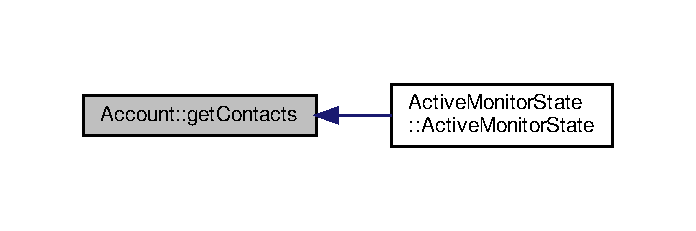
\includegraphics[width=334pt]{db/d22/class_account_a53a9e366a589538552a368e3bbac2fd3_icgraph}
\end{center}
\end{figure}
\mbox{\Hypertarget{class_account_a5117acc0c4ef7be21c5339bd9ae84e40}\label{class_account_a5117acc0c4ef7be21c5339bd9ae84e40}} 
\index{Account@{Account}!get\+Fences@{get\+Fences}}
\index{get\+Fences@{get\+Fences}!Account@{Account}}
\subsubsection{\texorpdfstring{get\+Fences()}{getFences()}}
{\footnotesize\ttfamily std\+::vector$<$ \hyperlink{class_fence}{Fence} $\ast$ $>$ \& Account\+::get\+Fences (\begin{DoxyParamCaption}{ }\end{DoxyParamCaption})}

Get the vector of the fences for this account. A public accessor to an otherwise private value.

\begin{DoxyReturn}{Returns}
a vector containing all the fence objects associated with this account 
\end{DoxyReturn}


Definition at line 105 of file Account.\+cpp.


\begin{DoxyCode}
106 \{
107     \textcolor{keywordflow}{return} \hyperlink{class_account_ad92a9e8008371f34da06cd416a716fa1}{fences};
108 \}
\end{DoxyCode}
Here is the caller graph for this function\+:
\nopagebreak
\begin{figure}[H]
\begin{center}
\leavevmode
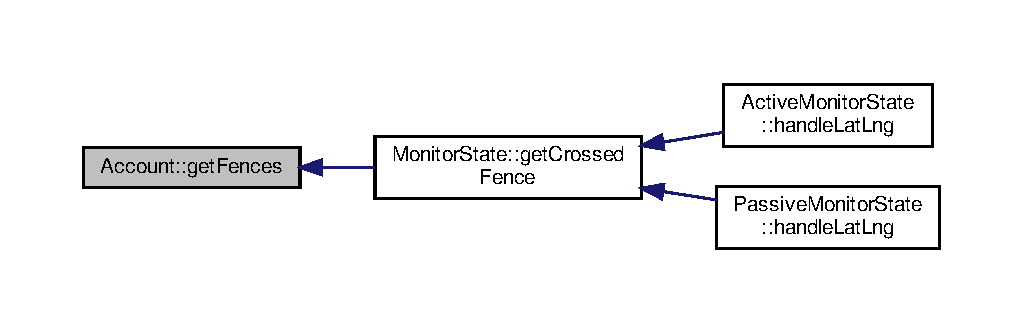
\includegraphics[width=350pt]{db/d22/class_account_a5117acc0c4ef7be21c5339bd9ae84e40_icgraph}
\end{center}
\end{figure}
\mbox{\Hypertarget{class_account_a1ef22885e8c6f145475c3306a4e6d74a}\label{class_account_a1ef22885e8c6f145475c3306a4e6d74a}} 
\index{Account@{Account}!get\+Name@{get\+Name}}
\index{get\+Name@{get\+Name}!Account@{Account}}
\subsubsection{\texorpdfstring{get\+Name()}{getName()}}
{\footnotesize\ttfamily std\+::string \& Account\+::get\+Name (\begin{DoxyParamCaption}{ }\end{DoxyParamCaption})}

A getter for the name of the account. A public accessor to an otherwise private value.

\begin{DoxyReturn}{Returns}
the name of the account. 
\end{DoxyReturn}


Definition at line 83 of file Account.\+cpp.


\begin{DoxyCode}
84 \{
85     \textcolor{keywordflow}{return} \hyperlink{class_account_a586e2c3461c5231eacf7c96851024a75}{name};
86 \}
\end{DoxyCode}
Here is the caller graph for this function\+:
\nopagebreak
\begin{figure}[H]
\begin{center}
\leavevmode
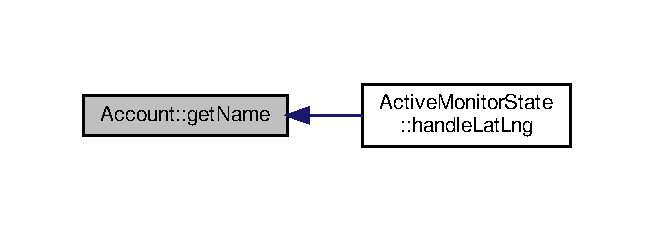
\includegraphics[width=314pt]{db/d22/class_account_a1ef22885e8c6f145475c3306a4e6d74a_icgraph}
\end{center}
\end{figure}
\mbox{\Hypertarget{class_account_a9ff3a257536bc933e0a39207bb89243d}\label{class_account_a9ff3a257536bc933e0a39207bb89243d}} 
\index{Account@{Account}!save\+Serialised\+Account@{save\+Serialised\+Account}}
\index{save\+Serialised\+Account@{save\+Serialised\+Account}!Account@{Account}}
\subsubsection{\texorpdfstring{save\+Serialised\+Account()}{saveSerialisedAccount()}}
{\footnotesize\ttfamily bool Account\+::save\+Serialised\+Account (\begin{DoxyParamCaption}\item[{const std\+::string \&}]{path }\end{DoxyParamCaption})}

Serialise the json account instance and output it.


\begin{DoxyParams}{Parameters}
{\em path} & the filepath of the J\+S\+ON file to save the serialised account to \\
\hline
\end{DoxyParams}
\begin{DoxyReturn}{Returns}
True if successful, false otherwise 
\end{DoxyReturn}


Definition at line 161 of file Account.\+cpp.


\begin{DoxyCode}
162 \{
163 
164     \textcolor{comment}{// Serialise the account instance.}
165     web::json::value jsonAccount = \hyperlink{class_account_a1e9b184e8a6ddf67e8814e6c575f657e}{serialiseAccount}();
166 
167     \textcolor{comment}{// Output the serialised json account to a file stream.}
168     utility::ofstream\_t of(path);
169     of << jsonAccount.serialize();
170     of.close();
171 
172     \textcolor{comment}{// We have successfully written to the file.}
173     \textcolor{keywordflow}{return} \textcolor{keyword}{true};
174 \}
\end{DoxyCode}
Here is the call graph for this function\+:
\nopagebreak
\begin{figure}[H]
\begin{center}
\leavevmode
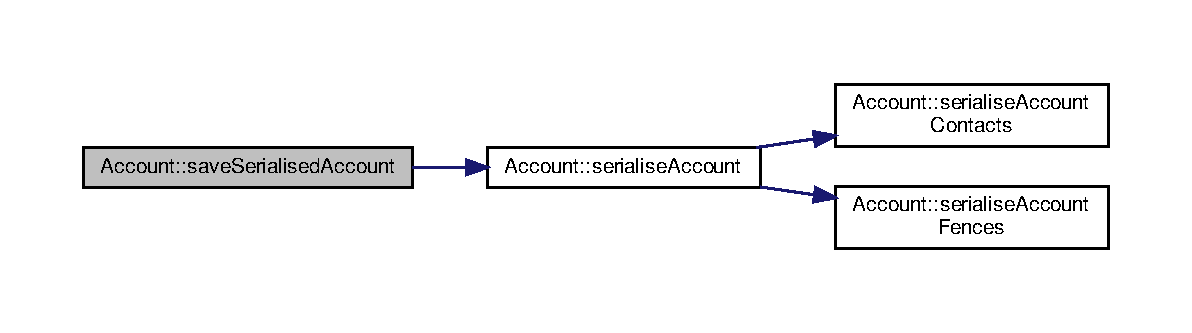
\includegraphics[width=350pt]{db/d22/class_account_a9ff3a257536bc933e0a39207bb89243d_cgraph}
\end{center}
\end{figure}
Here is the caller graph for this function\+:
\nopagebreak
\begin{figure}[H]
\begin{center}
\leavevmode
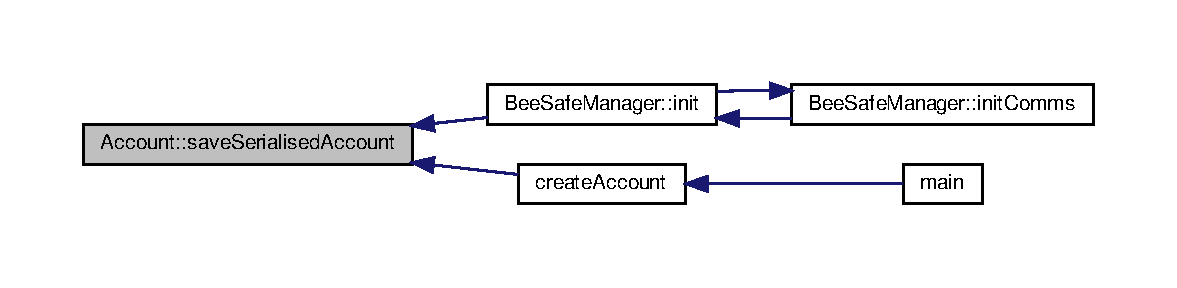
\includegraphics[width=350pt]{db/d22/class_account_a9ff3a257536bc933e0a39207bb89243d_icgraph}
\end{center}
\end{figure}
\mbox{\Hypertarget{class_account_a1e9b184e8a6ddf67e8814e6c575f657e}\label{class_account_a1e9b184e8a6ddf67e8814e6c575f657e}} 
\index{Account@{Account}!serialise\+Account@{serialise\+Account}}
\index{serialise\+Account@{serialise\+Account}!Account@{Account}}
\subsubsection{\texorpdfstring{serialise\+Account()}{serialiseAccount()}}
{\footnotesize\ttfamily web\+::json\+::value Account\+::serialise\+Account (\begin{DoxyParamCaption}{ }\end{DoxyParamCaption})}

Serialise the account object.

\begin{DoxyReturn}{Returns}
a json object containing the account object 
\end{DoxyReturn}


Definition at line 115 of file Account.\+cpp.


\begin{DoxyCode}
116 \{
117     web::json::value jsonAccount = web::json::value::object();
118     jsonAccount[utility::string\_t(U(\hyperlink{_account_8h_ac2f820be22c4390a71ec34abe54694c5}{JSON\_KEY\_ACCOUNT\_NAME}))]
119             = web::json::value::string(U(\hyperlink{class_account_a586e2c3461c5231eacf7c96851024a75}{name}));
120     jsonAccount[utility::string\_t(U(\hyperlink{_account_8h_a9a5dc301a4b04c85ce3b865530cd6ca7}{JSON\_KEY\_ACCOUNT\_CONTACTS}))]
121             = \hyperlink{class_account_a7f2d9836817ee851f723f6d3b1ff74a5}{serialiseAccountContacts}();
122     jsonAccount[utility::string\_t(U(\hyperlink{_account_8h_a83ba8a12dba5582a5a125d3ced877c6e}{JSON\_KEY\_ACCOUNT\_FENCES}))]
123             = \hyperlink{class_account_a426837a406852a6e6b11eda85828fc58}{serialiseAccountFences}();
124     \textcolor{keywordflow}{return} jsonAccount;
125 \}
\end{DoxyCode}
Here is the call graph for this function\+:
\nopagebreak
\begin{figure}[H]
\begin{center}
\leavevmode
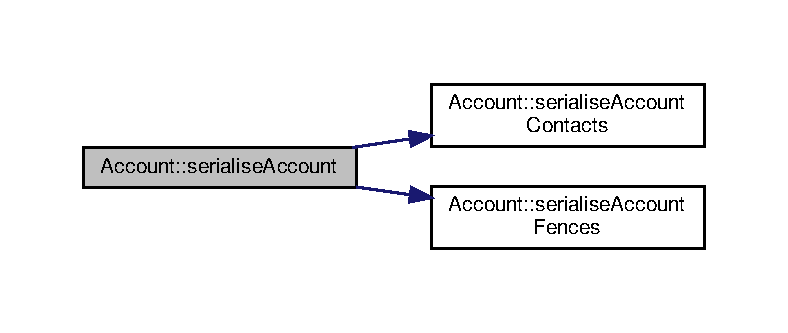
\includegraphics[width=350pt]{db/d22/class_account_a1e9b184e8a6ddf67e8814e6c575f657e_cgraph}
\end{center}
\end{figure}
Here is the caller graph for this function\+:
\nopagebreak
\begin{figure}[H]
\begin{center}
\leavevmode
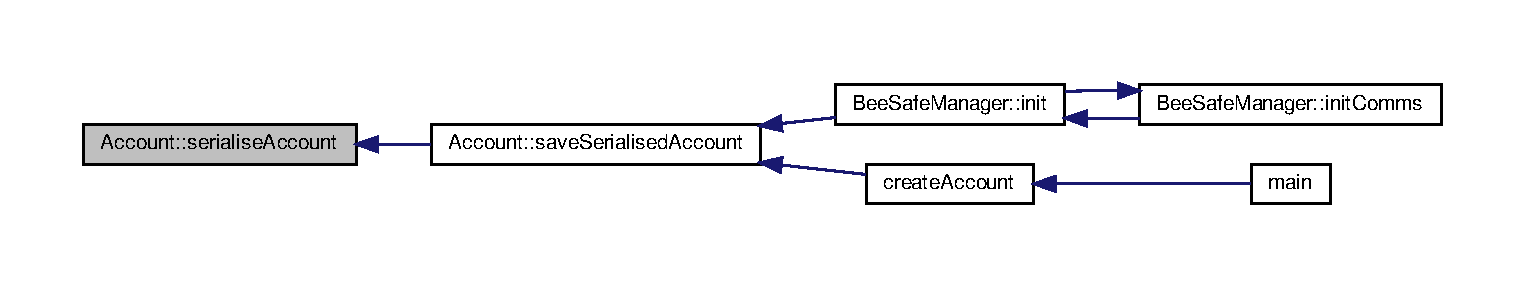
\includegraphics[width=350pt]{db/d22/class_account_a1e9b184e8a6ddf67e8814e6c575f657e_icgraph}
\end{center}
\end{figure}
\mbox{\Hypertarget{class_account_a7f2d9836817ee851f723f6d3b1ff74a5}\label{class_account_a7f2d9836817ee851f723f6d3b1ff74a5}} 
\index{Account@{Account}!serialise\+Account\+Contacts@{serialise\+Account\+Contacts}}
\index{serialise\+Account\+Contacts@{serialise\+Account\+Contacts}!Account@{Account}}
\subsubsection{\texorpdfstring{serialise\+Account\+Contacts()}{serialiseAccountContacts()}}
{\footnotesize\ttfamily web\+::json\+::value Account\+::serialise\+Account\+Contacts (\begin{DoxyParamCaption}{ }\end{DoxyParamCaption})}

Serialise the contacts for this account.

\begin{DoxyReturn}{Returns}
a json object containing the contacts for this account 
\end{DoxyReturn}


Definition at line 132 of file Account.\+cpp.


\begin{DoxyCode}
133 \{
134     web::json::value jsonContacts = web::json::value::array();
135     \textcolor{keywordflow}{for} (\textcolor{keywordtype}{int} i = 0; i < \hyperlink{class_account_aa4f77abd7c44f2a70b0cff8088e3491f}{contacts}.size(); ++i) \{
136         jsonContacts[i] = \hyperlink{class_account_aa4f77abd7c44f2a70b0cff8088e3491f}{contacts}[i]->serialiseContact();
137     \}
138     \textcolor{keywordflow}{return} jsonContacts;
139 \}
\end{DoxyCode}
Here is the caller graph for this function\+:
\nopagebreak
\begin{figure}[H]
\begin{center}
\leavevmode
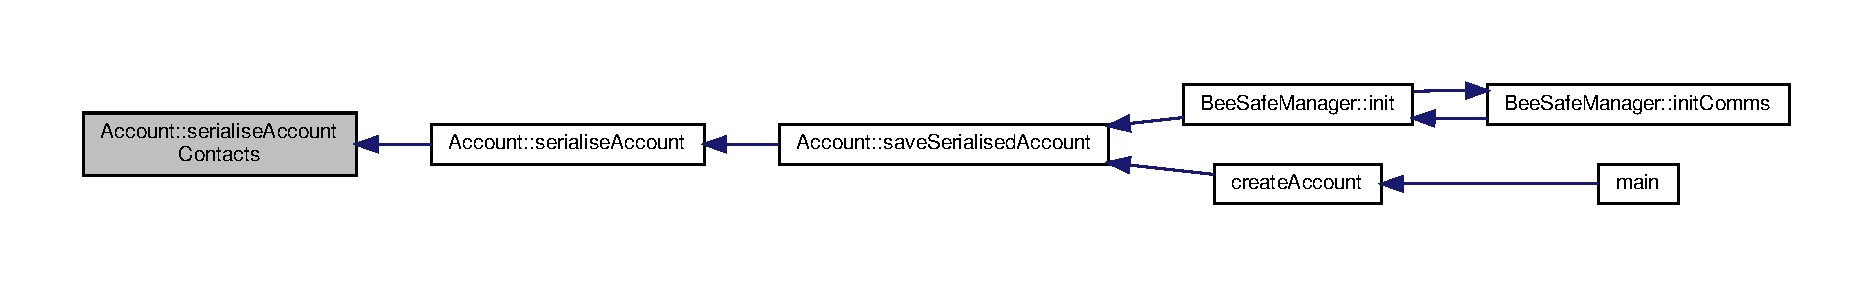
\includegraphics[width=350pt]{db/d22/class_account_a7f2d9836817ee851f723f6d3b1ff74a5_icgraph}
\end{center}
\end{figure}
\mbox{\Hypertarget{class_account_a426837a406852a6e6b11eda85828fc58}\label{class_account_a426837a406852a6e6b11eda85828fc58}} 
\index{Account@{Account}!serialise\+Account\+Fences@{serialise\+Account\+Fences}}
\index{serialise\+Account\+Fences@{serialise\+Account\+Fences}!Account@{Account}}
\subsubsection{\texorpdfstring{serialise\+Account\+Fences()}{serialiseAccountFences()}}
{\footnotesize\ttfamily web\+::json\+::value Account\+::serialise\+Account\+Fences (\begin{DoxyParamCaption}{ }\end{DoxyParamCaption})}

Serialise the fences for this account.

\begin{DoxyReturn}{Returns}
a J\+S\+ON object containing the fences for this account 
\end{DoxyReturn}


Definition at line 146 of file Account.\+cpp.


\begin{DoxyCode}
147 \{
148     web::json::value jsonFences = web::json::value::array();
149     \textcolor{keywordflow}{for} (\textcolor{keywordtype}{int} i = 0; i < \hyperlink{class_account_ad92a9e8008371f34da06cd416a716fa1}{fences}.size(); ++i) \{
150         jsonFences[i] = \hyperlink{class_account_ad92a9e8008371f34da06cd416a716fa1}{fences}[i]->serialiseFence();
151     \}
152     \textcolor{keywordflow}{return} jsonFences;
153 \}
\end{DoxyCode}
Here is the caller graph for this function\+:
\nopagebreak
\begin{figure}[H]
\begin{center}
\leavevmode
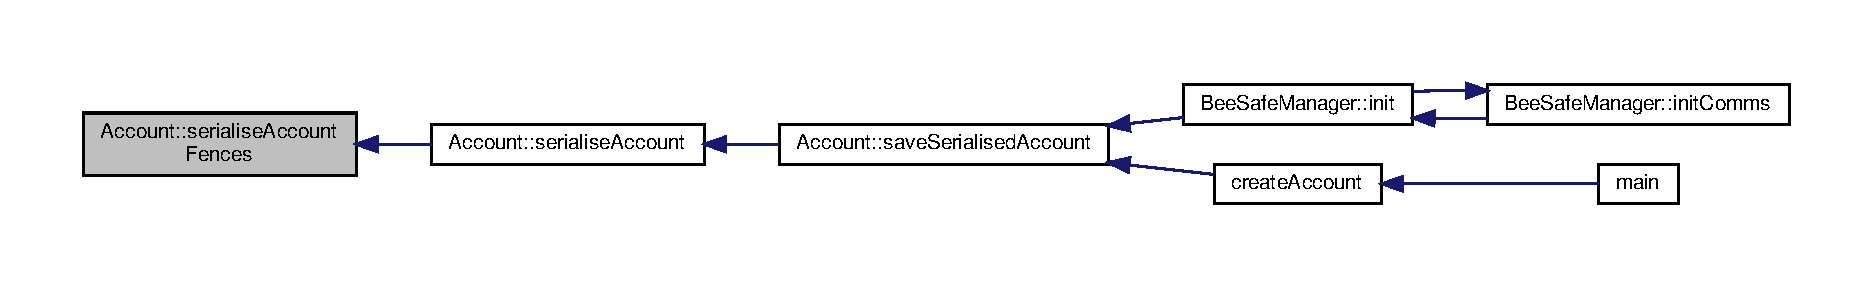
\includegraphics[width=350pt]{db/d22/class_account_a426837a406852a6e6b11eda85828fc58_icgraph}
\end{center}
\end{figure}


\subsection{Member Data Documentation}
\mbox{\Hypertarget{class_account_aa4f77abd7c44f2a70b0cff8088e3491f}\label{class_account_aa4f77abd7c44f2a70b0cff8088e3491f}} 
\index{Account@{Account}!contacts@{contacts}}
\index{contacts@{contacts}!Account@{Account}}
\subsubsection{\texorpdfstring{contacts}{contacts}}
{\footnotesize\ttfamily std\+::vector$<$\hyperlink{class_contact}{Contact}$\ast$$>$ Account\+::contacts\hspace{0.3cm}{\ttfamily [private]}}



Definition at line 78 of file Account.\+h.

\mbox{\Hypertarget{class_account_ad92a9e8008371f34da06cd416a716fa1}\label{class_account_ad92a9e8008371f34da06cd416a716fa1}} 
\index{Account@{Account}!fences@{fences}}
\index{fences@{fences}!Account@{Account}}
\subsubsection{\texorpdfstring{fences}{fences}}
{\footnotesize\ttfamily std\+::vector$<$\hyperlink{class_fence}{Fence}$\ast$$>$ Account\+::fences\hspace{0.3cm}{\ttfamily [private]}}



Definition at line 79 of file Account.\+h.

\mbox{\Hypertarget{class_account_a586e2c3461c5231eacf7c96851024a75}\label{class_account_a586e2c3461c5231eacf7c96851024a75}} 
\index{Account@{Account}!name@{name}}
\index{name@{name}!Account@{Account}}
\subsubsection{\texorpdfstring{name}{name}}
{\footnotesize\ttfamily std\+::string Account\+::name\hspace{0.3cm}{\ttfamily [private]}}



Definition at line 75 of file Account.\+h.



The documentation for this class was generated from the following files\+:\begin{DoxyCompactItemize}
\item 
software/\+Bee\+Safe\+P\+I/src/device/\hyperlink{_account_8h}{Account.\+h}\item 
software/\+Bee\+Safe\+P\+I/src/device/\hyperlink{_account_8cpp}{Account.\+cpp}\end{DoxyCompactItemize}

\hypertarget{class_account_builder}{}\doxysection{Account\+Builder Class Reference}
\label{class_account_builder}\index{AccountBuilder@{AccountBuilder}}


{\ttfamily \#include $<$Account\+Builder.\+h$>$}

\doxysubsection*{Public Member Functions}
\begin{DoxyCompactItemize}
\item 
\mbox{\hyperlink{class_account_builder_ae19ca737d825f1ecc99e8406a19a0699}{Account\+Builder}} (utility\+::stringstream\+\_\+t \&stream, std\+::error\+\_\+code \&error\+Code)
\item 
\mbox{\hyperlink{class_account}{Account}} $\ast$ \mbox{\hyperlink{class_account_builder_af44cc9897467096f65d3bd768fd01300}{build}} ()
\end{DoxyCompactItemize}


\doxysubsection{Constructor \& Destructor Documentation}
\mbox{\Hypertarget{class_account_builder_ae19ca737d825f1ecc99e8406a19a0699}\label{class_account_builder_ae19ca737d825f1ecc99e8406a19a0699}} 
\index{AccountBuilder@{AccountBuilder}!AccountBuilder@{AccountBuilder}}
\index{AccountBuilder@{AccountBuilder}!AccountBuilder@{AccountBuilder}}
\doxysubsubsection{\texorpdfstring{AccountBuilder()}{AccountBuilder()}}
{\footnotesize\ttfamily Account\+Builder\+::\+Account\+Builder (\begin{DoxyParamCaption}\item[{utility\+::stringstream\+\_\+t \&}]{stream,  }\item[{std\+::error\+\_\+code \&}]{error\+Code }\end{DoxyParamCaption})}



\doxysubsection{Member Function Documentation}
\mbox{\Hypertarget{class_account_builder_af44cc9897467096f65d3bd768fd01300}\label{class_account_builder_af44cc9897467096f65d3bd768fd01300}} 
\index{AccountBuilder@{AccountBuilder}!build@{build}}
\index{build@{build}!AccountBuilder@{AccountBuilder}}
\doxysubsubsection{\texorpdfstring{build()}{build()}}
{\footnotesize\ttfamily \mbox{\hyperlink{class_account}{Account}} $\ast$ Account\+Builder\+::build (\begin{DoxyParamCaption}{ }\end{DoxyParamCaption})}



The documentation for this class was generated from the following files\+:\begin{DoxyCompactItemize}
\item 
device/\mbox{\hyperlink{_account_builder_8h}{Account\+Builder.\+h}}\item 
device/\mbox{\hyperlink{_account_builder_8cpp}{Account\+Builder.\+cpp}}\end{DoxyCompactItemize}

\hypertarget{class_active_monitor_state}{}\section{Active\+Monitor\+State Class Reference}
\label{class_active_monitor_state}\index{Active\+Monitor\+State@{Active\+Monitor\+State}}


The active monitor state child class.  




{\ttfamily \#include $<$Active\+Monitor\+State.\+h$>$}



Inheritance diagram for Active\+Monitor\+State\+:
\nopagebreak
\begin{figure}[H]
\begin{center}
\leavevmode
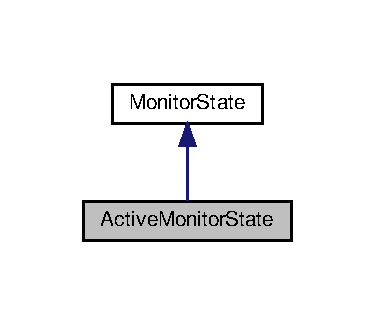
\includegraphics[width=180pt]{dd/d2b/class_active_monitor_state__inherit__graph}
\end{center}
\end{figure}


Collaboration diagram for Active\+Monitor\+State\+:
\nopagebreak
\begin{figure}[H]
\begin{center}
\leavevmode
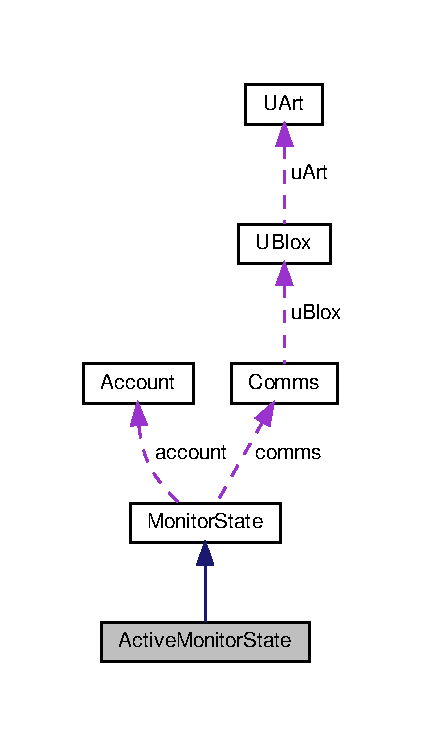
\includegraphics[width=205pt]{d5/d71/class_active_monitor_state__coll__graph}
\end{center}
\end{figure}
\subsection*{Public Member Functions}
\begin{DoxyCompactItemize}
\item 
\hyperlink{class_active_monitor_state_af1a0341307d63c900ccdc0a99fbe59e0}{Active\+Monitor\+State} (\hyperlink{class_comms}{Comms} $\ast$\hyperlink{class_monitor_state_a41914e9963c67ef2d17774f04bad3518}{comms}, \hyperlink{class_account}{Account} $\ast$\hyperlink{class_monitor_state_a41128d4942ec0d5b107c63d1d95af811}{account})
\item 
\hyperlink{class_active_monitor_state_accb86642ec52bae9aacd2aa4e9ff4410}{$\sim$\+Active\+Monitor\+State} () override
\item 
bool \hyperlink{class_active_monitor_state_a4566e7e96a777df86ab78ec326b551d0}{is\+Perimeter\+Crossed} ()
\item 
std\+::chrono\+::time\+\_\+point$<$ std\+::chrono\+::steady\+\_\+clock $>$ \hyperlink{class_active_monitor_state_ab94dede8d2e407aaddb0df056f5a329c}{get\+Since\+Perimeter\+Crossed} ()
\item 
std\+::vector$<$ std\+::pair$<$ \hyperlink{class_contact}{Contact} $\ast$, bool $>$ $>$ \& \hyperlink{class_active_monitor_state_ac1d5b33105abe5bd68ed5ee0396bc3be}{get\+Sent\+Notifications} ()
\item 
\hyperlink{class_monitor_state}{Monitor\+State} $\ast$ \hyperlink{class_active_monitor_state_a0eb7622ad3aa4d372d90589838cb50a9}{handle\+Lat\+Lng} (std\+::pair$<$ double, double $>$ \&lat\+Lng) override
\end{DoxyCompactItemize}
\subsection*{Private Member Functions}
\begin{DoxyCompactItemize}
\item 
bool \hyperlink{class_active_monitor_state_add557ab0dd0774482c08c982b82395e7}{all\+Notifications\+Sent} ()
\item 
void \hyperlink{class_active_monitor_state_adedd023d280922991a5dd980017549ec}{set\+Sent\+Notifications} (bool sent)
\item 
void \hyperlink{class_active_monitor_state_aae5b3a425c74e7017446be277d69c06d}{send\+Message\+Notifications} (bool force\+All, std\+::string \&message)
\end{DoxyCompactItemize}
\subsection*{Private Attributes}
\begin{DoxyCompactItemize}
\item 
bool \hyperlink{class_active_monitor_state_af4c93e1be350ea9cf4ac97f97abaf79e}{perimeter\+Crossed}
\item 
std\+::chrono\+::time\+\_\+point$<$ std\+::chrono\+::steady\+\_\+clock $>$ \hyperlink{class_active_monitor_state_a4313399b0922fccd66ecea2fcf77c08f}{since\+Perimeter\+Crossed}
\item 
std\+::vector$<$ std\+::pair$<$ \hyperlink{class_contact}{Contact} $\ast$, bool $>$ $>$ \hyperlink{class_active_monitor_state_a25493a87079926faf7d03b8587ad9f62}{sent\+Notifications}
\end{DoxyCompactItemize}
\subsection*{Additional Inherited Members}


\subsection{Detailed Description}
The active monitor state child class. 

The child class to \hyperlink{class_monitor_state}{Monitor\+State}. It handles the functionality of what to do when the device is outside a fence, by defining how to handle notifications, and constantly monitoring if the device returns to the fence to hand over to the \hyperlink{class_passive_monitor_state}{Passive\+Monitor\+State} class.

\begin{DoxyAuthor}{Author}
Bee\+Safe Team, Team 13
\end{DoxyAuthor}
\begin{DoxyVersion}{Version}
v1.\+0
\end{DoxyVersion}
\begin{DoxyDate}{Date}
\$\+Date\+: 2020/04/20
\end{DoxyDate}
\hyperlink{class_contact}{Contact}\+: \href{mailto:beesafe.uofg@gmail.com}{\tt beesafe.\+uofg@gmail.\+com}

Licence\+: M\+IT

The child class to \hyperlink{class_monitor_state}{Monitor\+State}. It handles the functionality of what to do when the device is outside a fence, by defining how to handle notifications, and constantly monitoring if the device returns to the fence to hand over to the \hyperlink{class_passive_monitor_state}{Passive\+Monitor\+State} class.

\begin{DoxyAuthor}{Author}
Bee\+Safe Team, Team 13
\end{DoxyAuthor}
\begin{DoxyVersion}{Version}
v1.\+0
\end{DoxyVersion}
\begin{DoxyDate}{Date}
2020/04/20
\end{DoxyDate}
\hyperlink{class_contact}{Contact}\+: \href{mailto:beesafe.uofg@gmail.com}{\tt beesafe.\+uofg@gmail.\+com}

Licence\+: M\+IT 

Definition at line 46 of file Active\+Monitor\+State.\+h.



\subsection{Constructor \& Destructor Documentation}
\mbox{\Hypertarget{class_active_monitor_state_af1a0341307d63c900ccdc0a99fbe59e0}\label{class_active_monitor_state_af1a0341307d63c900ccdc0a99fbe59e0}} 
\index{Active\+Monitor\+State@{Active\+Monitor\+State}!Active\+Monitor\+State@{Active\+Monitor\+State}}
\index{Active\+Monitor\+State@{Active\+Monitor\+State}!Active\+Monitor\+State@{Active\+Monitor\+State}}
\subsubsection{\texorpdfstring{Active\+Monitor\+State()}{ActiveMonitorState()}}
{\footnotesize\ttfamily Active\+Monitor\+State\+::\+Active\+Monitor\+State (\begin{DoxyParamCaption}\item[{\hyperlink{class_comms}{Comms} $\ast$}]{comms,  }\item[{\hyperlink{class_account}{Account} $\ast$}]{account }\end{DoxyParamCaption})}



Definition at line 35 of file Active\+Monitor\+State.\+cpp.


\begin{DoxyCode}
36         : \hyperlink{class_monitor_state_ace027ab9e5703ac4e4b808eeebc3c961}{MonitorState}(\hyperlink{_active_monitor_state_8h_a9fdfa2faf1d746d8aa632437fd3bd03c}{ACTIVE\_STATE\_NAME}, comms, account)
37 \{
38 
39     \textcolor{comment}{// By definition the device just crossed the perimeter.}
40     \hyperlink{class_active_monitor_state_af4c93e1be350ea9cf4ac97f97abaf79e}{perimeterCrossed} = \textcolor{keyword}{true};
41     \hyperlink{class_active_monitor_state_a4313399b0922fccd66ecea2fcf77c08f}{sincePerimeterCrossed} = std::chrono::steady\_clock::now();
42 
43     \textcolor{comment}{// Populate the notifications.}
44     \textcolor{keywordflow}{for} (\hyperlink{class_contact}{Contact} *contact : account->\hyperlink{class_account_a53a9e366a589538552a368e3bbac2fd3}{getContacts}()) \{
45         \hyperlink{class_active_monitor_state_a25493a87079926faf7d03b8587ad9f62}{sentNotifications}.emplace\_back(std::make\_pair(contact, \textcolor{keyword}{false}));
46     \}
47 \}
\end{DoxyCode}
Here is the call graph for this function\+:
\nopagebreak
\begin{figure}[H]
\begin{center}
\leavevmode
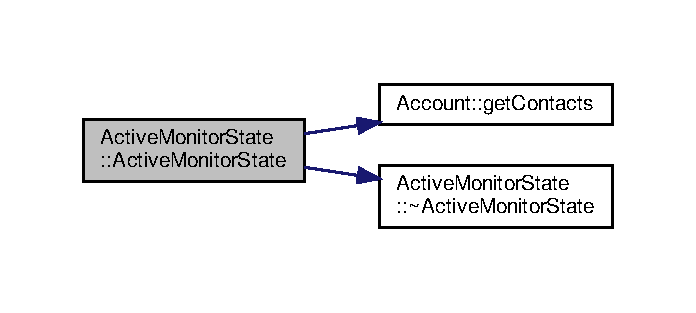
\includegraphics[width=334pt]{d9/db8/class_active_monitor_state_af1a0341307d63c900ccdc0a99fbe59e0_cgraph}
\end{center}
\end{figure}
\mbox{\Hypertarget{class_active_monitor_state_accb86642ec52bae9aacd2aa4e9ff4410}\label{class_active_monitor_state_accb86642ec52bae9aacd2aa4e9ff4410}} 
\index{Active\+Monitor\+State@{Active\+Monitor\+State}!````~Active\+Monitor\+State@{$\sim$\+Active\+Monitor\+State}}
\index{````~Active\+Monitor\+State@{$\sim$\+Active\+Monitor\+State}!Active\+Monitor\+State@{Active\+Monitor\+State}}
\subsubsection{\texorpdfstring{$\sim$\+Active\+Monitor\+State()}{~ActiveMonitorState()}}
{\footnotesize\ttfamily Active\+Monitor\+State\+::$\sim$\+Active\+Monitor\+State (\begin{DoxyParamCaption}{ }\end{DoxyParamCaption})\hspace{0.3cm}{\ttfamily [override]}, {\ttfamily [default]}}

Here is the caller graph for this function\+:
\nopagebreak
\begin{figure}[H]
\begin{center}
\leavevmode
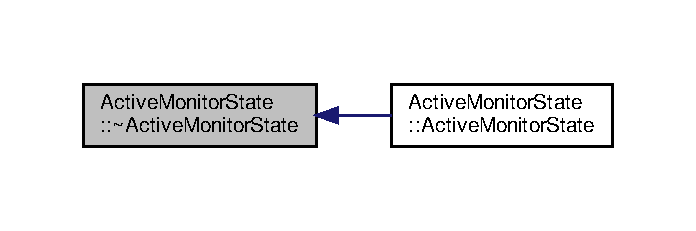
\includegraphics[width=334pt]{d9/db8/class_active_monitor_state_accb86642ec52bae9aacd2aa4e9ff4410_icgraph}
\end{center}
\end{figure}


\subsection{Member Function Documentation}
\mbox{\Hypertarget{class_active_monitor_state_add557ab0dd0774482c08c982b82395e7}\label{class_active_monitor_state_add557ab0dd0774482c08c982b82395e7}} 
\index{Active\+Monitor\+State@{Active\+Monitor\+State}!all\+Notifications\+Sent@{all\+Notifications\+Sent}}
\index{all\+Notifications\+Sent@{all\+Notifications\+Sent}!Active\+Monitor\+State@{Active\+Monitor\+State}}
\subsubsection{\texorpdfstring{all\+Notifications\+Sent()}{allNotificationsSent()}}
{\footnotesize\ttfamily bool Active\+Monitor\+State\+::all\+Notifications\+Sent (\begin{DoxyParamCaption}{ }\end{DoxyParamCaption})\hspace{0.3cm}{\ttfamily [private]}}



Definition at line 67 of file Active\+Monitor\+State.\+cpp.


\begin{DoxyCode}
68 \{
69     \textcolor{keywordflow}{for} (\textcolor{keyword}{auto}& notifiableContact : \hyperlink{class_active_monitor_state_a25493a87079926faf7d03b8587ad9f62}{sentNotifications}) \{
70         \textcolor{keywordflow}{if} (!notifiableContact.second) \{
71             \textcolor{keywordflow}{return} \textcolor{keyword}{false};
72         \}
73     \}
74     \textcolor{keywordflow}{return} \textcolor{keyword}{true};
75 \}
\end{DoxyCode}
Here is the caller graph for this function\+:
\nopagebreak
\begin{figure}[H]
\begin{center}
\leavevmode
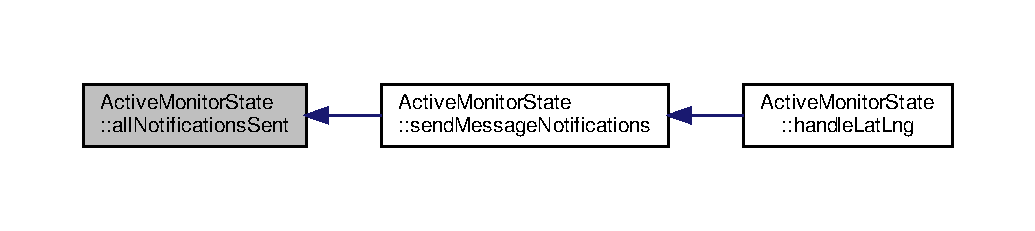
\includegraphics[width=350pt]{d9/db8/class_active_monitor_state_add557ab0dd0774482c08c982b82395e7_icgraph}
\end{center}
\end{figure}
\mbox{\Hypertarget{class_active_monitor_state_ac1d5b33105abe5bd68ed5ee0396bc3be}\label{class_active_monitor_state_ac1d5b33105abe5bd68ed5ee0396bc3be}} 
\index{Active\+Monitor\+State@{Active\+Monitor\+State}!get\+Sent\+Notifications@{get\+Sent\+Notifications}}
\index{get\+Sent\+Notifications@{get\+Sent\+Notifications}!Active\+Monitor\+State@{Active\+Monitor\+State}}
\subsubsection{\texorpdfstring{get\+Sent\+Notifications()}{getSentNotifications()}}
{\footnotesize\ttfamily std\+::vector$<$ std\+::pair$<$ \hyperlink{class_contact}{Contact} $\ast$, bool $>$ $>$ \& Active\+Monitor\+State\+::get\+Sent\+Notifications (\begin{DoxyParamCaption}{ }\end{DoxyParamCaption})}



Definition at line 62 of file Active\+Monitor\+State.\+cpp.


\begin{DoxyCode}
63 \{
64     \textcolor{keywordflow}{return} \hyperlink{class_active_monitor_state_a25493a87079926faf7d03b8587ad9f62}{sentNotifications};
65 \}
\end{DoxyCode}
\mbox{\Hypertarget{class_active_monitor_state_ab94dede8d2e407aaddb0df056f5a329c}\label{class_active_monitor_state_ab94dede8d2e407aaddb0df056f5a329c}} 
\index{Active\+Monitor\+State@{Active\+Monitor\+State}!get\+Since\+Perimeter\+Crossed@{get\+Since\+Perimeter\+Crossed}}
\index{get\+Since\+Perimeter\+Crossed@{get\+Since\+Perimeter\+Crossed}!Active\+Monitor\+State@{Active\+Monitor\+State}}
\subsubsection{\texorpdfstring{get\+Since\+Perimeter\+Crossed()}{getSincePerimeterCrossed()}}
{\footnotesize\ttfamily std\+::chrono\+::time\+\_\+point$<$ std\+::chrono\+::steady\+\_\+clock $>$ Active\+Monitor\+State\+::get\+Since\+Perimeter\+Crossed (\begin{DoxyParamCaption}{ }\end{DoxyParamCaption})}



Definition at line 57 of file Active\+Monitor\+State.\+cpp.


\begin{DoxyCode}
58 \{
59     \textcolor{keywordflow}{return} \hyperlink{class_active_monitor_state_a4313399b0922fccd66ecea2fcf77c08f}{sincePerimeterCrossed};
60 \}
\end{DoxyCode}
\mbox{\Hypertarget{class_active_monitor_state_a0eb7622ad3aa4d372d90589838cb50a9}\label{class_active_monitor_state_a0eb7622ad3aa4d372d90589838cb50a9}} 
\index{Active\+Monitor\+State@{Active\+Monitor\+State}!handle\+Lat\+Lng@{handle\+Lat\+Lng}}
\index{handle\+Lat\+Lng@{handle\+Lat\+Lng}!Active\+Monitor\+State@{Active\+Monitor\+State}}
\subsubsection{\texorpdfstring{handle\+Lat\+Lng()}{handleLatLng()}}
{\footnotesize\ttfamily \hyperlink{class_monitor_state}{Monitor\+State} $\ast$ Active\+Monitor\+State\+::handle\+Lat\+Lng (\begin{DoxyParamCaption}\item[{std\+::pair$<$ double, double $>$ \&}]{lat\+Lng }\end{DoxyParamCaption})\hspace{0.3cm}{\ttfamily [override]}, {\ttfamily [virtual]}}



Implements \hyperlink{class_monitor_state_a8c8b871e3e8308e11f35905dd8741878}{Monitor\+State}.



Definition at line 108 of file Active\+Monitor\+State.\+cpp.


\begin{DoxyCode}
109 \{
110     \textcolor{comment}{// Get the fence the device has left.}
111     std::cout << \textcolor{stringliteral}{"Checking fences..."} << std::endl;
112     \hyperlink{class_fence}{Fence}* crossedFence = \hyperlink{class_monitor_state_a332c5f42bf46cd217e36f300e5279766}{getCrossedFence}(latLng);
113     \textcolor{keywordtype}{bool} inside = crossedFence == \textcolor{keyword}{nullptr};
114 
115     \textcolor{comment}{// If the fence has been crossed, update the monitor states.}
116     \textcolor{keywordflow}{if} (inside != \hyperlink{class_active_monitor_state_af4c93e1be350ea9cf4ac97f97abaf79e}{perimeterCrossed}) \{
117         std::cout << \textcolor{stringliteral}{"Switching from state "} << \hyperlink{class_active_monitor_state_af4c93e1be350ea9cf4ac97f97abaf79e}{perimeterCrossed} << \textcolor{stringliteral}{" to state "} << inside 
      << std::endl;
118         \hyperlink{class_active_monitor_state_af4c93e1be350ea9cf4ac97f97abaf79e}{perimeterCrossed} = inside;
119         \hyperlink{class_active_monitor_state_a4313399b0922fccd66ecea2fcf77c08f}{sincePerimeterCrossed} = std::chrono::steady\_clock::now();
120         \hyperlink{class_active_monitor_state_adedd023d280922991a5dd980017549ec}{setSentNotifications}(\textcolor{keyword}{false});
121     \}
122     std::cout << \textcolor{stringliteral}{"... fence checks complete."} << std::endl;
123 
124     \textcolor{comment}{// Elapsed seconds since monitor (perimeterCrossed) state change.}
125     \textcolor{keyword}{auto} now = std::chrono::steady\_clock::now();
126     \textcolor{keywordtype}{long} \textcolor{keywordtype}{long} \textcolor{keywordtype}{int} elapsedSec = std::chrono::duration\_cast<std::chrono::seconds>
127             (now - \hyperlink{class_active_monitor_state_a4313399b0922fccd66ecea2fcf77c08f}{sincePerimeterCrossed}).count();
128 
129     \textcolor{comment}{// Handle notifications.}
130     \textcolor{keywordflow}{if} (inside && elapsedSec > \hyperlink{_active_monitor_state_8cpp_af734ccbfe87f3ed675b4836ae5761dbb}{STEPPED\_INSIDE\_NOTIFICATION\_DELAY\_SEC}) 
      \{
131 
132         \textcolor{comment}{// Send a message informing the contacts that the device has returned.}
133         std::cout << \textcolor{stringliteral}{"Notifying contacts (back inside) ..."} << std::endl;
134         std::string message = \textcolor{stringliteral}{"Device "} + \hyperlink{class_monitor_state_a41128d4942ec0d5b107c63d1d95af811}{account}->\hyperlink{class_account_a1ef22885e8c6f145475c3306a4e6d74a}{getName}() + \textcolor{stringliteral}{" has returned to the fence."};
135         \hyperlink{class_active_monitor_state_aae5b3a425c74e7017446be277d69c06d}{sendMessageNotifications}(\textcolor{keyword}{true}, message);
136         std::cout << \textcolor{stringliteral}{"... contacts successfully notified (back inside)."} << std::endl;
137 
138     \} \textcolor{keywordflow}{else} \textcolor{keywordflow}{if} (!inside && elapsedSec > \hyperlink{_active_monitor_state_8cpp_a61900fdfa0a56947870551db86143a1c}{STEPPED\_OUTSIDE\_NOTIFICATION\_DELAY\_SEC}
      ) \{
139 
140         \textcolor{comment}{// Send a message informing the contacts that the device has left the fence.}
141         std::cout << \textcolor{stringliteral}{"Notifying contacts (outside) ..."} << std::endl;
142         std::string message = \textcolor{stringliteral}{"Device "} + \hyperlink{class_monitor_state_a41128d4942ec0d5b107c63d1d95af811}{account}->\hyperlink{class_account_a1ef22885e8c6f145475c3306a4e6d74a}{getName}()
143                               + \textcolor{stringliteral}{" has left fence "} + crossedFence->\hyperlink{class_fence_a1d90d0ff61bec6cda8240f6365fc5d28}{getName}() + \textcolor{stringliteral}{"."};
144         \hyperlink{class_active_monitor_state_aae5b3a425c74e7017446be277d69c06d}{sendMessageNotifications}(\textcolor{keyword}{false}, message);
145         std::cout << \textcolor{stringliteral}{"... contacts successfully notified (outside)."} << std::endl;
146 
147     \}
148 
149     \textcolor{comment}{// If the device has reentered the fence and parents have been notified, switch.}
150     \textcolor{keywordflow}{return} inside && elapsedSec > \hyperlink{_active_monitor_state_8cpp_af734ccbfe87f3ed675b4836ae5761dbb}{STEPPED\_INSIDE\_NOTIFICATION\_DELAY\_SEC}
151            ? \textcolor{keyword}{new} \hyperlink{class_passive_monitor_state}{PassiveMonitorState}(\hyperlink{class_monitor_state_a41914e9963c67ef2d17774f04bad3518}{comms}, \hyperlink{class_monitor_state_a41128d4942ec0d5b107c63d1d95af811}{account})
152            : nullptr;
153 \}
\end{DoxyCode}
Here is the call graph for this function\+:
\nopagebreak
\begin{figure}[H]
\begin{center}
\leavevmode
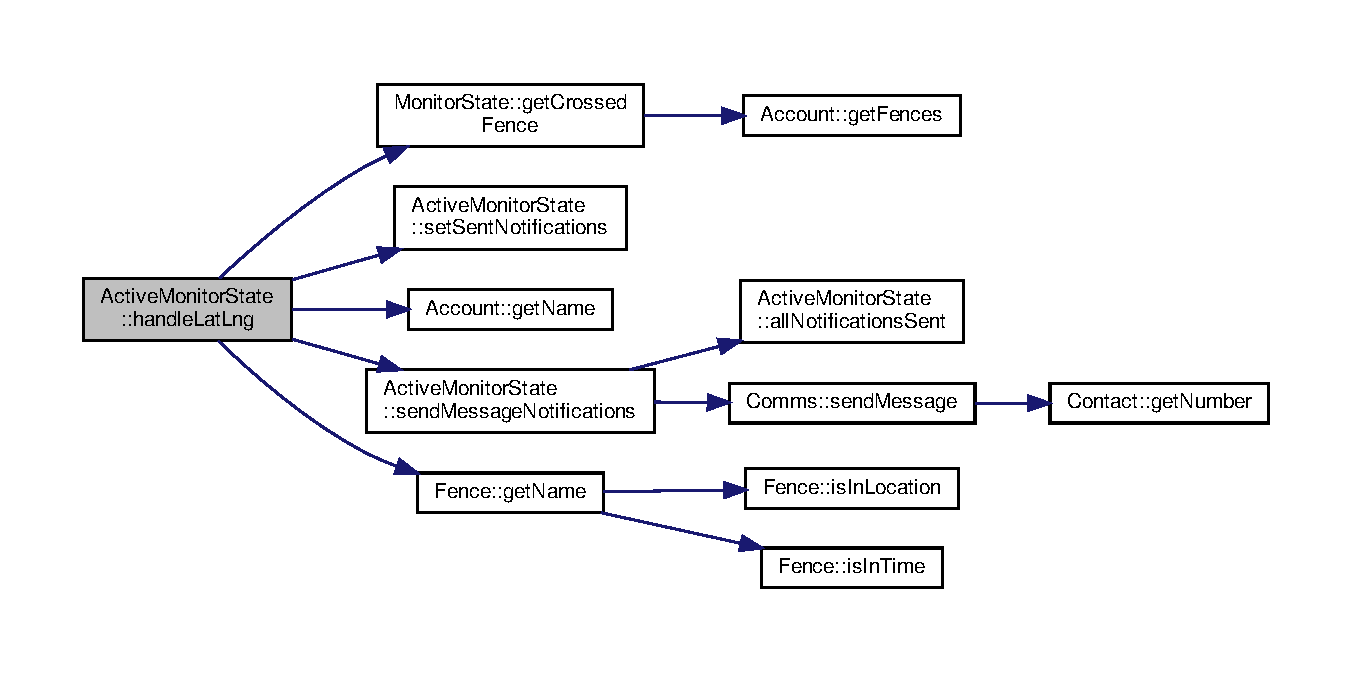
\includegraphics[width=350pt]{d9/db8/class_active_monitor_state_a0eb7622ad3aa4d372d90589838cb50a9_cgraph}
\end{center}
\end{figure}
\mbox{\Hypertarget{class_active_monitor_state_a4566e7e96a777df86ab78ec326b551d0}\label{class_active_monitor_state_a4566e7e96a777df86ab78ec326b551d0}} 
\index{Active\+Monitor\+State@{Active\+Monitor\+State}!is\+Perimeter\+Crossed@{is\+Perimeter\+Crossed}}
\index{is\+Perimeter\+Crossed@{is\+Perimeter\+Crossed}!Active\+Monitor\+State@{Active\+Monitor\+State}}
\subsubsection{\texorpdfstring{is\+Perimeter\+Crossed()}{isPerimeterCrossed()}}
{\footnotesize\ttfamily bool Active\+Monitor\+State\+::is\+Perimeter\+Crossed (\begin{DoxyParamCaption}{ }\end{DoxyParamCaption})}



Definition at line 52 of file Active\+Monitor\+State.\+cpp.


\begin{DoxyCode}
53 \{
54     \textcolor{keywordflow}{return} \hyperlink{class_active_monitor_state_af4c93e1be350ea9cf4ac97f97abaf79e}{perimeterCrossed};
55 \}
\end{DoxyCode}
\mbox{\Hypertarget{class_active_monitor_state_aae5b3a425c74e7017446be277d69c06d}\label{class_active_monitor_state_aae5b3a425c74e7017446be277d69c06d}} 
\index{Active\+Monitor\+State@{Active\+Monitor\+State}!send\+Message\+Notifications@{send\+Message\+Notifications}}
\index{send\+Message\+Notifications@{send\+Message\+Notifications}!Active\+Monitor\+State@{Active\+Monitor\+State}}
\subsubsection{\texorpdfstring{send\+Message\+Notifications()}{sendMessageNotifications()}}
{\footnotesize\ttfamily void Active\+Monitor\+State\+::send\+Message\+Notifications (\begin{DoxyParamCaption}\item[{bool}]{force\+All,  }\item[{std\+::string \&}]{message }\end{DoxyParamCaption})\hspace{0.3cm}{\ttfamily [private]}}



Definition at line 84 of file Active\+Monitor\+State.\+cpp.


\begin{DoxyCode}
85 \{
86     \textcolor{comment}{// Check that all contacts have been notified.}
87     \textcolor{keywordflow}{if} (!forceAll && \hyperlink{class_active_monitor_state_add557ab0dd0774482c08c982b82395e7}{allNotificationsSent}()) \{
88         std::cout << \textcolor{stringliteral}{"All contacts already notified."} << std::endl;
89         \textcolor{keywordflow}{return};
90     \}
91 
92     \textcolor{comment}{// Notify contacts.}
93     \textcolor{keywordflow}{for} (\textcolor{keyword}{auto} &notifiableContact : \hyperlink{class_active_monitor_state_a25493a87079926faf7d03b8587ad9f62}{sentNotifications}) \{
94         \textcolor{keywordflow}{if} (!notifiableContact.second || forceAll) \{
95 
96             \textcolor{comment}{// Notify the contact.}
97             std::cout << \textcolor{stringliteral}{"Notifying contact "}
98                       << notifiableContact.first->getForename()
99                       << \textcolor{stringliteral}{" "} << notifiableContact.first->getSurname()
100                       << \textcolor{stringliteral}{"... "};
101             notifiableContact.second = \hyperlink{class_monitor_state_a41914e9963c67ef2d17774f04bad3518}{comms}->\hyperlink{class_comms_a30ab10ea604ab2b169ca66f3f1071c0e}{sendMessage}(*notifiableContact.first, message
      );
102             std::cout << (notifiableContact.second ? \textcolor{stringliteral}{"Success!"} : \textcolor{stringliteral}{"Failed!"}) << std::endl;
103 
104         \}
105     \}
106 \}
\end{DoxyCode}
Here is the call graph for this function\+:
\nopagebreak
\begin{figure}[H]
\begin{center}
\leavevmode
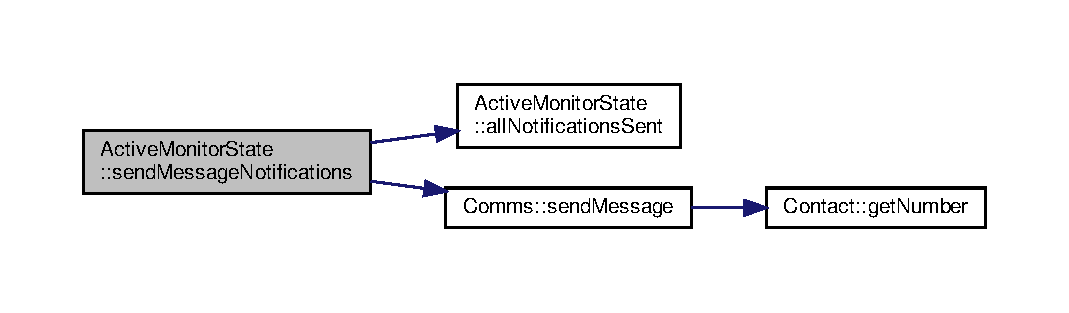
\includegraphics[width=350pt]{d9/db8/class_active_monitor_state_aae5b3a425c74e7017446be277d69c06d_cgraph}
\end{center}
\end{figure}
Here is the caller graph for this function\+:
\nopagebreak
\begin{figure}[H]
\begin{center}
\leavevmode
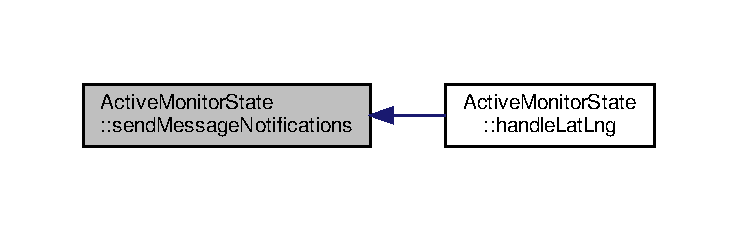
\includegraphics[width=350pt]{d9/db8/class_active_monitor_state_aae5b3a425c74e7017446be277d69c06d_icgraph}
\end{center}
\end{figure}
\mbox{\Hypertarget{class_active_monitor_state_adedd023d280922991a5dd980017549ec}\label{class_active_monitor_state_adedd023d280922991a5dd980017549ec}} 
\index{Active\+Monitor\+State@{Active\+Monitor\+State}!set\+Sent\+Notifications@{set\+Sent\+Notifications}}
\index{set\+Sent\+Notifications@{set\+Sent\+Notifications}!Active\+Monitor\+State@{Active\+Monitor\+State}}
\subsubsection{\texorpdfstring{set\+Sent\+Notifications()}{setSentNotifications()}}
{\footnotesize\ttfamily void Active\+Monitor\+State\+::set\+Sent\+Notifications (\begin{DoxyParamCaption}\item[{bool}]{sent }\end{DoxyParamCaption})\hspace{0.3cm}{\ttfamily [private]}}



Definition at line 77 of file Active\+Monitor\+State.\+cpp.


\begin{DoxyCode}
78 \{
79     \textcolor{keywordflow}{for} (\textcolor{keyword}{auto}& notifiableContact : \hyperlink{class_active_monitor_state_a25493a87079926faf7d03b8587ad9f62}{sentNotifications}) \{
80         notifiableContact.second = sent;
81     \}
82 \}
\end{DoxyCode}
Here is the caller graph for this function\+:
\nopagebreak
\begin{figure}[H]
\begin{center}
\leavevmode
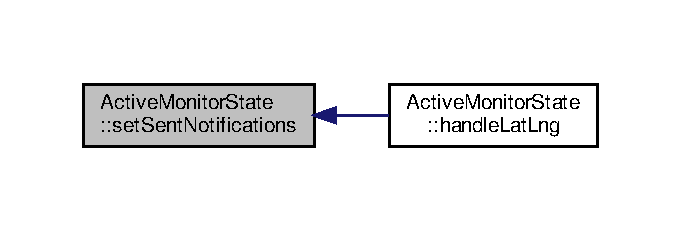
\includegraphics[width=327pt]{d9/db8/class_active_monitor_state_adedd023d280922991a5dd980017549ec_icgraph}
\end{center}
\end{figure}


\subsection{Member Data Documentation}
\mbox{\Hypertarget{class_active_monitor_state_af4c93e1be350ea9cf4ac97f97abaf79e}\label{class_active_monitor_state_af4c93e1be350ea9cf4ac97f97abaf79e}} 
\index{Active\+Monitor\+State@{Active\+Monitor\+State}!perimeter\+Crossed@{perimeter\+Crossed}}
\index{perimeter\+Crossed@{perimeter\+Crossed}!Active\+Monitor\+State@{Active\+Monitor\+State}}
\subsubsection{\texorpdfstring{perimeter\+Crossed}{perimeterCrossed}}
{\footnotesize\ttfamily bool Active\+Monitor\+State\+::perimeter\+Crossed\hspace{0.3cm}{\ttfamily [private]}}



Definition at line 77 of file Active\+Monitor\+State.\+h.

\mbox{\Hypertarget{class_active_monitor_state_a25493a87079926faf7d03b8587ad9f62}\label{class_active_monitor_state_a25493a87079926faf7d03b8587ad9f62}} 
\index{Active\+Monitor\+State@{Active\+Monitor\+State}!sent\+Notifications@{sent\+Notifications}}
\index{sent\+Notifications@{sent\+Notifications}!Active\+Monitor\+State@{Active\+Monitor\+State}}
\subsubsection{\texorpdfstring{sent\+Notifications}{sentNotifications}}
{\footnotesize\ttfamily std\+::vector$<$std\+::pair$<$\hyperlink{class_contact}{Contact}$\ast$, bool$>$ $>$ Active\+Monitor\+State\+::sent\+Notifications\hspace{0.3cm}{\ttfamily [private]}}



Definition at line 81 of file Active\+Monitor\+State.\+h.

\mbox{\Hypertarget{class_active_monitor_state_a4313399b0922fccd66ecea2fcf77c08f}\label{class_active_monitor_state_a4313399b0922fccd66ecea2fcf77c08f}} 
\index{Active\+Monitor\+State@{Active\+Monitor\+State}!since\+Perimeter\+Crossed@{since\+Perimeter\+Crossed}}
\index{since\+Perimeter\+Crossed@{since\+Perimeter\+Crossed}!Active\+Monitor\+State@{Active\+Monitor\+State}}
\subsubsection{\texorpdfstring{since\+Perimeter\+Crossed}{sincePerimeterCrossed}}
{\footnotesize\ttfamily std\+::chrono\+::time\+\_\+point$<$std\+::chrono\+::steady\+\_\+clock$>$ Active\+Monitor\+State\+::since\+Perimeter\+Crossed\hspace{0.3cm}{\ttfamily [private]}}



Definition at line 78 of file Active\+Monitor\+State.\+h.



The documentation for this class was generated from the following files\+:\begin{DoxyCompactItemize}
\item 
software/\+Bee\+Safe\+P\+I/src/monitor/states/\hyperlink{_active_monitor_state_8h}{Active\+Monitor\+State.\+h}\item 
software/\+Bee\+Safe\+P\+I/src/monitor/states/\hyperlink{_active_monitor_state_8cpp}{Active\+Monitor\+State.\+cpp}\end{DoxyCompactItemize}

\hypertarget{class_bee_safe_manager}{}\section{Bee\+Safe\+Manager Class Reference}
\label{class_bee_safe_manager}\index{Bee\+Safe\+Manager@{Bee\+Safe\+Manager}}


The Bee\+Safe class initiates the complete program.  




{\ttfamily \#include $<$Bee\+Safe.\+h$>$}



Collaboration diagram for Bee\+Safe\+Manager\+:\nopagebreak
\begin{figure}[H]
\begin{center}
\leavevmode
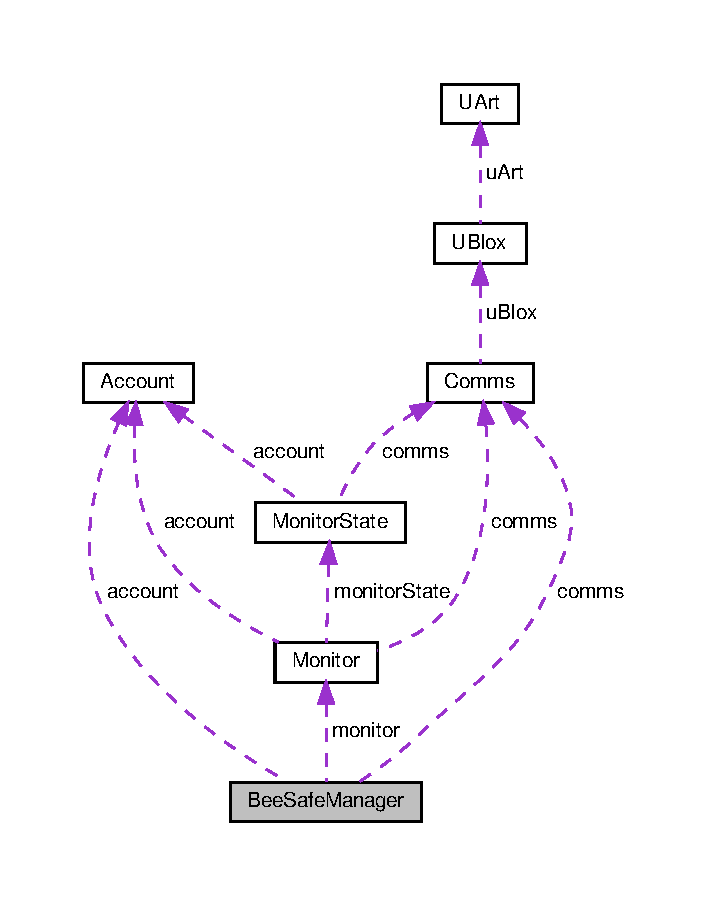
\includegraphics[width=341pt]{d7/d13/class_bee_safe_manager__coll__graph}
\end{center}
\end{figure}
\subsection*{Public Member Functions}
\begin{DoxyCompactItemize}
\item 
\hyperlink{class_bee_safe_manager_a4a897d6317bdc548fb235d0cdb2877b1}{Bee\+Safe\+Manager} ()
\item 
\hyperlink{class_bee_safe_manager_ac99fb148bcac3aa3f51e96fdf7bc0c1b}{$\sim$\+Bee\+Safe\+Manager} ()
\item 
\hyperlink{class_comms}{Comms} $\ast$const \hyperlink{class_bee_safe_manager_a8c4c98723335cfcc179fcbf3f8c3d9d3}{get\+Comms} ()
\item 
\hyperlink{class_monitor}{Monitor} $\ast$const \hyperlink{class_bee_safe_manager_acc33322594eea80e4b4b21e580713c00}{get\+Monitor} ()
\item 
\hyperlink{class_account}{Account} $\ast$const \hyperlink{class_bee_safe_manager_a4052276ed4263cdbe715ce115e1ccee2}{get\+Account} ()
\item 
bool \hyperlink{class_bee_safe_manager_a2f16b09c454e21c887d14ac5483973cf}{init} ()
\item 
bool \hyperlink{class_bee_safe_manager_a7242d89761621de0e09ec9ea360fca27}{start} ()
\end{DoxyCompactItemize}
\subsection*{Private Member Functions}
\begin{DoxyCompactItemize}
\item 
\hyperlink{class_comms}{Comms} $\ast$ \hyperlink{class_bee_safe_manager_a28306d7ccf7136a6086d666f4ebb6566}{init\+Comms} ()
\item 
\hyperlink{class_monitor}{Monitor} $\ast$ \hyperlink{class_bee_safe_manager_ad30babe45ead2cb6a5b0559afa5bc5ff}{init\+Monitor} (\hyperlink{class_comms}{Comms} $\ast$\hyperlink{class_bee_safe_manager_a80b19afbb679d08be14d67a45447f9e1}{comms})
\item 
\hyperlink{class_account}{Account} $\ast$ \hyperlink{class_bee_safe_manager_a7395aeacd246ce69c65f255a2eab1d04}{init\+Account} (const char $\ast$path)
\end{DoxyCompactItemize}
\subsection*{Private Attributes}
\begin{DoxyCompactItemize}
\item 
\hyperlink{class_comms}{Comms} $\ast$ \hyperlink{class_bee_safe_manager_a80b19afbb679d08be14d67a45447f9e1}{comms}
\item 
\hyperlink{class_monitor}{Monitor} $\ast$ \hyperlink{class_bee_safe_manager_a3b885b4fb364228c914095f2e670f9af}{monitor}
\item 
\hyperlink{class_account}{Account} $\ast$ \hyperlink{class_bee_safe_manager_a52bc9bc8c1ea9608b83d603b142443b0}{account}
\end{DoxyCompactItemize}


\subsection{Detailed Description}
The Bee\+Safe class initiates the complete program. 

The Bee\+Safe class creates the instances of classes required to communicate with the hardware, the monitors overseeing that, and the account information to whom the system must reach out in case of an emergency. Containing the \hyperlink{_bee_safe_8cpp_ae66f6b31b5ad750f1fe042a706a4e3d4}{main()} function, this is the root of the Bee\+Safe A\+PI.

\begin{DoxyAuthor}{Author}
Bee\+Safe Team, Team 13
\end{DoxyAuthor}
\begin{DoxyVersion}{Version}
v1.\+0
\end{DoxyVersion}
\begin{DoxyDate}{Date}
2020/04/20
\end{DoxyDate}
\hyperlink{class_contact}{Contact}\+: \href{mailto:beesafe.uofg@gmail.com}{\tt beesafe.\+uofg@gmail.\+com}

Licence\+: M\+IT 

Definition at line 34 of file Bee\+Safe.\+h.



\subsection{Constructor \& Destructor Documentation}
\mbox{\Hypertarget{class_bee_safe_manager_a4a897d6317bdc548fb235d0cdb2877b1}\label{class_bee_safe_manager_a4a897d6317bdc548fb235d0cdb2877b1}} 
\index{Bee\+Safe\+Manager@{Bee\+Safe\+Manager}!Bee\+Safe\+Manager@{Bee\+Safe\+Manager}}
\index{Bee\+Safe\+Manager@{Bee\+Safe\+Manager}!Bee\+Safe\+Manager@{Bee\+Safe\+Manager}}
\subsubsection{\texorpdfstring{Bee\+Safe\+Manager()}{BeeSafeManager()}}
{\footnotesize\ttfamily Bee\+Safe\+Manager\+::\+Bee\+Safe\+Manager (\begin{DoxyParamCaption}{ }\end{DoxyParamCaption})}

Constructor used to initialise an instance of the \hyperlink{class_bee_safe_manager}{Bee\+Safe\+Manager} class. 

Definition at line 41 of file Bee\+Safe.\+cpp.


\begin{DoxyCode}
42 \{
43     \hyperlink{class_bee_safe_manager_a80b19afbb679d08be14d67a45447f9e1}{comms} = \textcolor{keyword}{nullptr};
44     \hyperlink{class_bee_safe_manager_a52bc9bc8c1ea9608b83d603b142443b0}{account} = \textcolor{keyword}{nullptr};
45     \hyperlink{class_bee_safe_manager_a3b885b4fb364228c914095f2e670f9af}{monitor} = \textcolor{keyword}{nullptr};
46 \}
\end{DoxyCode}
Here is the caller graph for this function\+:\nopagebreak
\begin{figure}[H]
\begin{center}
\leavevmode
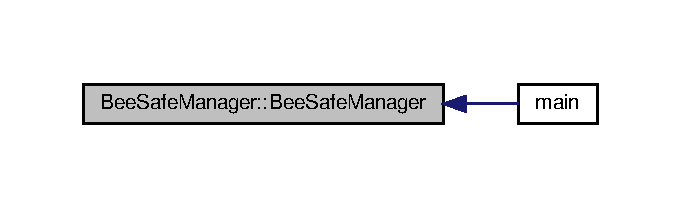
\includegraphics[width=327pt]{d5/d75/class_bee_safe_manager_a4a897d6317bdc548fb235d0cdb2877b1_icgraph}
\end{center}
\end{figure}
\mbox{\Hypertarget{class_bee_safe_manager_ac99fb148bcac3aa3f51e96fdf7bc0c1b}\label{class_bee_safe_manager_ac99fb148bcac3aa3f51e96fdf7bc0c1b}} 
\index{Bee\+Safe\+Manager@{Bee\+Safe\+Manager}!````~Bee\+Safe\+Manager@{$\sim$\+Bee\+Safe\+Manager}}
\index{````~Bee\+Safe\+Manager@{$\sim$\+Bee\+Safe\+Manager}!Bee\+Safe\+Manager@{Bee\+Safe\+Manager}}
\subsubsection{\texorpdfstring{$\sim$\+Bee\+Safe\+Manager()}{~BeeSafeManager()}}
{\footnotesize\ttfamily Bee\+Safe\+Manager\+::$\sim$\+Bee\+Safe\+Manager (\begin{DoxyParamCaption}{ }\end{DoxyParamCaption})}

Destructor is responsible for releasing any resources occupied by the \hyperlink{class_bee_safe_manager}{Bee\+Safe\+Manager} instance. Note, if the monitor thread is running, it will implicitly be stopped. 

Definition at line 52 of file Bee\+Safe.\+cpp.


\begin{DoxyCode}
53 \{
54     \textcolor{comment}{// Delete monitor first to illegal memory access.}
55     \textcolor{keywordflow}{if} (\hyperlink{class_bee_safe_manager_a3b885b4fb364228c914095f2e670f9af}{monitor} != \textcolor{keyword}{nullptr}) \{
56         \hyperlink{class_bee_safe_manager_a3b885b4fb364228c914095f2e670f9af}{monitor}->\hyperlink{class_monitor_a2d2e309666c98333a317c9786f94f6ad}{join}();
57         \textcolor{keyword}{delete} \hyperlink{class_bee_safe_manager_a3b885b4fb364228c914095f2e670f9af}{monitor};
58     \}
59 
60     \textcolor{comment}{// Finally, delete the comms and account.}
61     \textcolor{keyword}{delete} \hyperlink{class_bee_safe_manager_a80b19afbb679d08be14d67a45447f9e1}{comms};
62     \textcolor{keyword}{delete} \hyperlink{class_bee_safe_manager_a52bc9bc8c1ea9608b83d603b142443b0}{account};
63 \}
\end{DoxyCode}
Here is the call graph for this function\+:\nopagebreak
\begin{figure}[H]
\begin{center}
\leavevmode
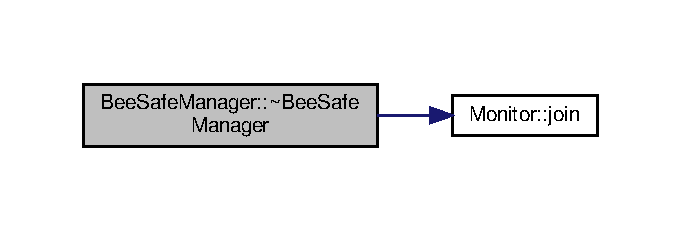
\includegraphics[width=327pt]{d5/d75/class_bee_safe_manager_ac99fb148bcac3aa3f51e96fdf7bc0c1b_cgraph}
\end{center}
\end{figure}


\subsection{Member Function Documentation}
\mbox{\Hypertarget{class_bee_safe_manager_a4052276ed4263cdbe715ce115e1ccee2}\label{class_bee_safe_manager_a4052276ed4263cdbe715ce115e1ccee2}} 
\index{Bee\+Safe\+Manager@{Bee\+Safe\+Manager}!get\+Account@{get\+Account}}
\index{get\+Account@{get\+Account}!Bee\+Safe\+Manager@{Bee\+Safe\+Manager}}
\subsubsection{\texorpdfstring{get\+Account()}{getAccount()}}
{\footnotesize\ttfamily \hyperlink{class_account}{Account} $\ast$const Bee\+Safe\+Manager\+::get\+Account (\begin{DoxyParamCaption}{ }\end{DoxyParamCaption})}

Get the device \hyperlink{class_account}{Account} being monitored.

\begin{DoxyReturn}{Returns}
A pointer to an \hyperlink{class_account}{Account} instance (if initialised), nullptr otherwise. 
\end{DoxyReturn}


Definition at line 90 of file Bee\+Safe.\+cpp.


\begin{DoxyCode}
91 \{
92     \textcolor{keywordflow}{return} \hyperlink{class_bee_safe_manager_a52bc9bc8c1ea9608b83d603b142443b0}{account};
93 \}
\end{DoxyCode}
\mbox{\Hypertarget{class_bee_safe_manager_a8c4c98723335cfcc179fcbf3f8c3d9d3}\label{class_bee_safe_manager_a8c4c98723335cfcc179fcbf3f8c3d9d3}} 
\index{Bee\+Safe\+Manager@{Bee\+Safe\+Manager}!get\+Comms@{get\+Comms}}
\index{get\+Comms@{get\+Comms}!Bee\+Safe\+Manager@{Bee\+Safe\+Manager}}
\subsubsection{\texorpdfstring{get\+Comms()}{getComms()}}
{\footnotesize\ttfamily \hyperlink{class_comms}{Comms} $\ast$const Bee\+Safe\+Manager\+::get\+Comms (\begin{DoxyParamCaption}{ }\end{DoxyParamCaption})}

Get the managers communication interface.

\begin{DoxyReturn}{Returns}
A pointer to the \hyperlink{class_comms}{Comms} interface instance (if initialised), a nullptr otherwise. 
\end{DoxyReturn}


Definition at line 70 of file Bee\+Safe.\+cpp.


\begin{DoxyCode}
71 \{
72     \textcolor{keywordflow}{return} \hyperlink{class_bee_safe_manager_a80b19afbb679d08be14d67a45447f9e1}{comms};
73 \}
\end{DoxyCode}
\mbox{\Hypertarget{class_bee_safe_manager_acc33322594eea80e4b4b21e580713c00}\label{class_bee_safe_manager_acc33322594eea80e4b4b21e580713c00}} 
\index{Bee\+Safe\+Manager@{Bee\+Safe\+Manager}!get\+Monitor@{get\+Monitor}}
\index{get\+Monitor@{get\+Monitor}!Bee\+Safe\+Manager@{Bee\+Safe\+Manager}}
\subsubsection{\texorpdfstring{get\+Monitor()}{getMonitor()}}
{\footnotesize\ttfamily \hyperlink{class_monitor}{Monitor} $\ast$const Bee\+Safe\+Manager\+::get\+Monitor (\begin{DoxyParamCaption}{ }\end{DoxyParamCaption})}

Get the monitor thread responsible for checking the users location.

\begin{DoxyReturn}{Returns}
A pointer to the \hyperlink{class_monitor}{Monitor} thread (if initialised), nullptr otherwise. 
\end{DoxyReturn}


Definition at line 80 of file Bee\+Safe.\+cpp.


\begin{DoxyCode}
81 \{
82     \textcolor{keywordflow}{return} \hyperlink{class_bee_safe_manager_a3b885b4fb364228c914095f2e670f9af}{monitor};
83 \}
\end{DoxyCode}
\mbox{\Hypertarget{class_bee_safe_manager_a2f16b09c454e21c887d14ac5483973cf}\label{class_bee_safe_manager_a2f16b09c454e21c887d14ac5483973cf}} 
\index{Bee\+Safe\+Manager@{Bee\+Safe\+Manager}!init@{init}}
\index{init@{init}!Bee\+Safe\+Manager@{Bee\+Safe\+Manager}}
\subsubsection{\texorpdfstring{init()}{init()}}
{\footnotesize\ttfamily bool Bee\+Safe\+Manager\+::init (\begin{DoxyParamCaption}{ }\end{DoxyParamCaption})}

Attempt to initialise the \hyperlink{class_bee_safe_manager}{Bee\+Safe\+Manager} instance responsible for managing the monitor thread, comms and accounts. Note, the function will only set the member pointers in the event all necessary sub-\/systems are initialised.

Furthermore, because an account may not be already present on the device, the resulting member account pointer {\itshape may be a nullptr}.

\begin{DoxyReturn}{Returns}
True if all necessary components have been initialised, false otherwise. 
\end{DoxyReturn}


Definition at line 107 of file Bee\+Safe.\+cpp.


\begin{DoxyCode}
108 \{
109     \textcolor{comment}{// Prevent memory leaks by releasing occupied resources.}
110     \textcolor{keywordflow}{if} (this->\hyperlink{class_bee_safe_manager_a3b885b4fb364228c914095f2e670f9af}{monitor} != \textcolor{keyword}{nullptr}) \{
111         this->\hyperlink{class_bee_safe_manager_a3b885b4fb364228c914095f2e670f9af}{monitor}->\hyperlink{class_monitor_a2d2e309666c98333a317c9786f94f6ad}{join}();
112         \textcolor{keyword}{delete} this->\hyperlink{class_bee_safe_manager_a3b885b4fb364228c914095f2e670f9af}{monitor};
113     \}
114     \textcolor{keyword}{delete} this->\hyperlink{class_bee_safe_manager_a80b19afbb679d08be14d67a45447f9e1}{comms};
115     \textcolor{keyword}{delete} this->\hyperlink{class_bee_safe_manager_a52bc9bc8c1ea9608b83d603b142443b0}{account};
116 
117     \textcolor{comment}{// First, attempt to init comms.}
118     std::cout << \textcolor{stringliteral}{"Initialising comms interface..."} << std::endl;
119     \textcolor{keyword}{auto} \hyperlink{class_bee_safe_manager_a80b19afbb679d08be14d67a45447f9e1}{comms} = \hyperlink{class_bee_safe_manager_a28306d7ccf7136a6086d666f4ebb6566}{initComms}();
120     \textcolor{keywordflow}{if} (\hyperlink{class_bee_safe_manager_a80b19afbb679d08be14d67a45447f9e1}{comms} == \textcolor{keyword}{nullptr}) \{
121         std::cerr << \textcolor{stringliteral}{"Failed to initialise comms interface."} << std::endl;
122         \textcolor{keywordflow}{return} \textcolor{keyword}{false};
123     \}
124     std::cout << \textcolor{stringliteral}{"... comms interface successfully initialised."} << std::endl;
125     
126     \textcolor{comment}{// Attempt to initialise the monitor thread.}
127     std::cout << \textcolor{stringliteral}{"Initialising monitor thread..."} << std::endl;
128     \textcolor{keyword}{auto} \hyperlink{class_bee_safe_manager_a3b885b4fb364228c914095f2e670f9af}{monitor} = \hyperlink{class_bee_safe_manager_ad30babe45ead2cb6a5b0559afa5bc5ff}{initMonitor}(\hyperlink{class_bee_safe_manager_a80b19afbb679d08be14d67a45447f9e1}{comms});
129     \textcolor{keywordflow}{if} (\hyperlink{class_bee_safe_manager_a3b885b4fb364228c914095f2e670f9af}{monitor} == \textcolor{keyword}{nullptr}) \{
130         std::cerr << \textcolor{stringliteral}{"Failed to initialise monitor thread."} << std::endl;
131         \textcolor{keyword}{delete} \hyperlink{class_bee_safe_manager_a80b19afbb679d08be14d67a45447f9e1}{comms};
132         \textcolor{keywordflow}{return} \textcolor{keyword}{false};
133     \}
134     std::cout << \textcolor{stringliteral}{"... monitor thread successfully initialised."} << std::endl;
135 
136     \textcolor{comment}{// The account can be null.}
137     std::cout << \textcolor{stringliteral}{"Initialising account..."} << std::endl;
138     \textcolor{keyword}{auto} \hyperlink{class_bee_safe_manager_a52bc9bc8c1ea9608b83d603b142443b0}{account} = \hyperlink{class_bee_safe_manager_a7395aeacd246ce69c65f255a2eab1d04}{initAccount}(\hyperlink{_bee_safe_8cpp_aeadb35b2afa47797b56f17423460fad8}{ACCOUNT\_PATH});
139     \textcolor{keywordflow}{if} (\hyperlink{class_bee_safe_manager_a52bc9bc8c1ea9608b83d603b142443b0}{account} == \textcolor{keyword}{nullptr}) \{
140         std::cerr << \textcolor{stringliteral}{"Failed to initialise account."} << std::endl;
141     \} \textcolor{keywordflow}{else} \{
142         \hyperlink{class_bee_safe_manager_a52bc9bc8c1ea9608b83d603b142443b0}{account}->\hyperlink{class_account_a9ff3a257536bc933e0a39207bb89243d}{saveSerialisedAccount}(\textcolor{stringliteral}{"../../data/Account\_Verif.json"});
143         std::cout << \textcolor{stringliteral}{"... account successfully initialised."} << std::endl;
144     \}
145 
146     \textcolor{comment}{// We have successfully initialised the manager.}
147     this->\hyperlink{class_bee_safe_manager_a80b19afbb679d08be14d67a45447f9e1}{comms} = \hyperlink{class_bee_safe_manager_a80b19afbb679d08be14d67a45447f9e1}{comms};
148     this->\hyperlink{class_bee_safe_manager_a3b885b4fb364228c914095f2e670f9af}{monitor} = \hyperlink{class_bee_safe_manager_a3b885b4fb364228c914095f2e670f9af}{monitor};
149     this->\hyperlink{class_bee_safe_manager_a52bc9bc8c1ea9608b83d603b142443b0}{account} = \hyperlink{class_bee_safe_manager_a52bc9bc8c1ea9608b83d603b142443b0}{account};
150 
151     \textcolor{keywordflow}{return} \textcolor{keyword}{true};
152 \}
\end{DoxyCode}
Here is the call graph for this function\+:\nopagebreak
\begin{figure}[H]
\begin{center}
\leavevmode
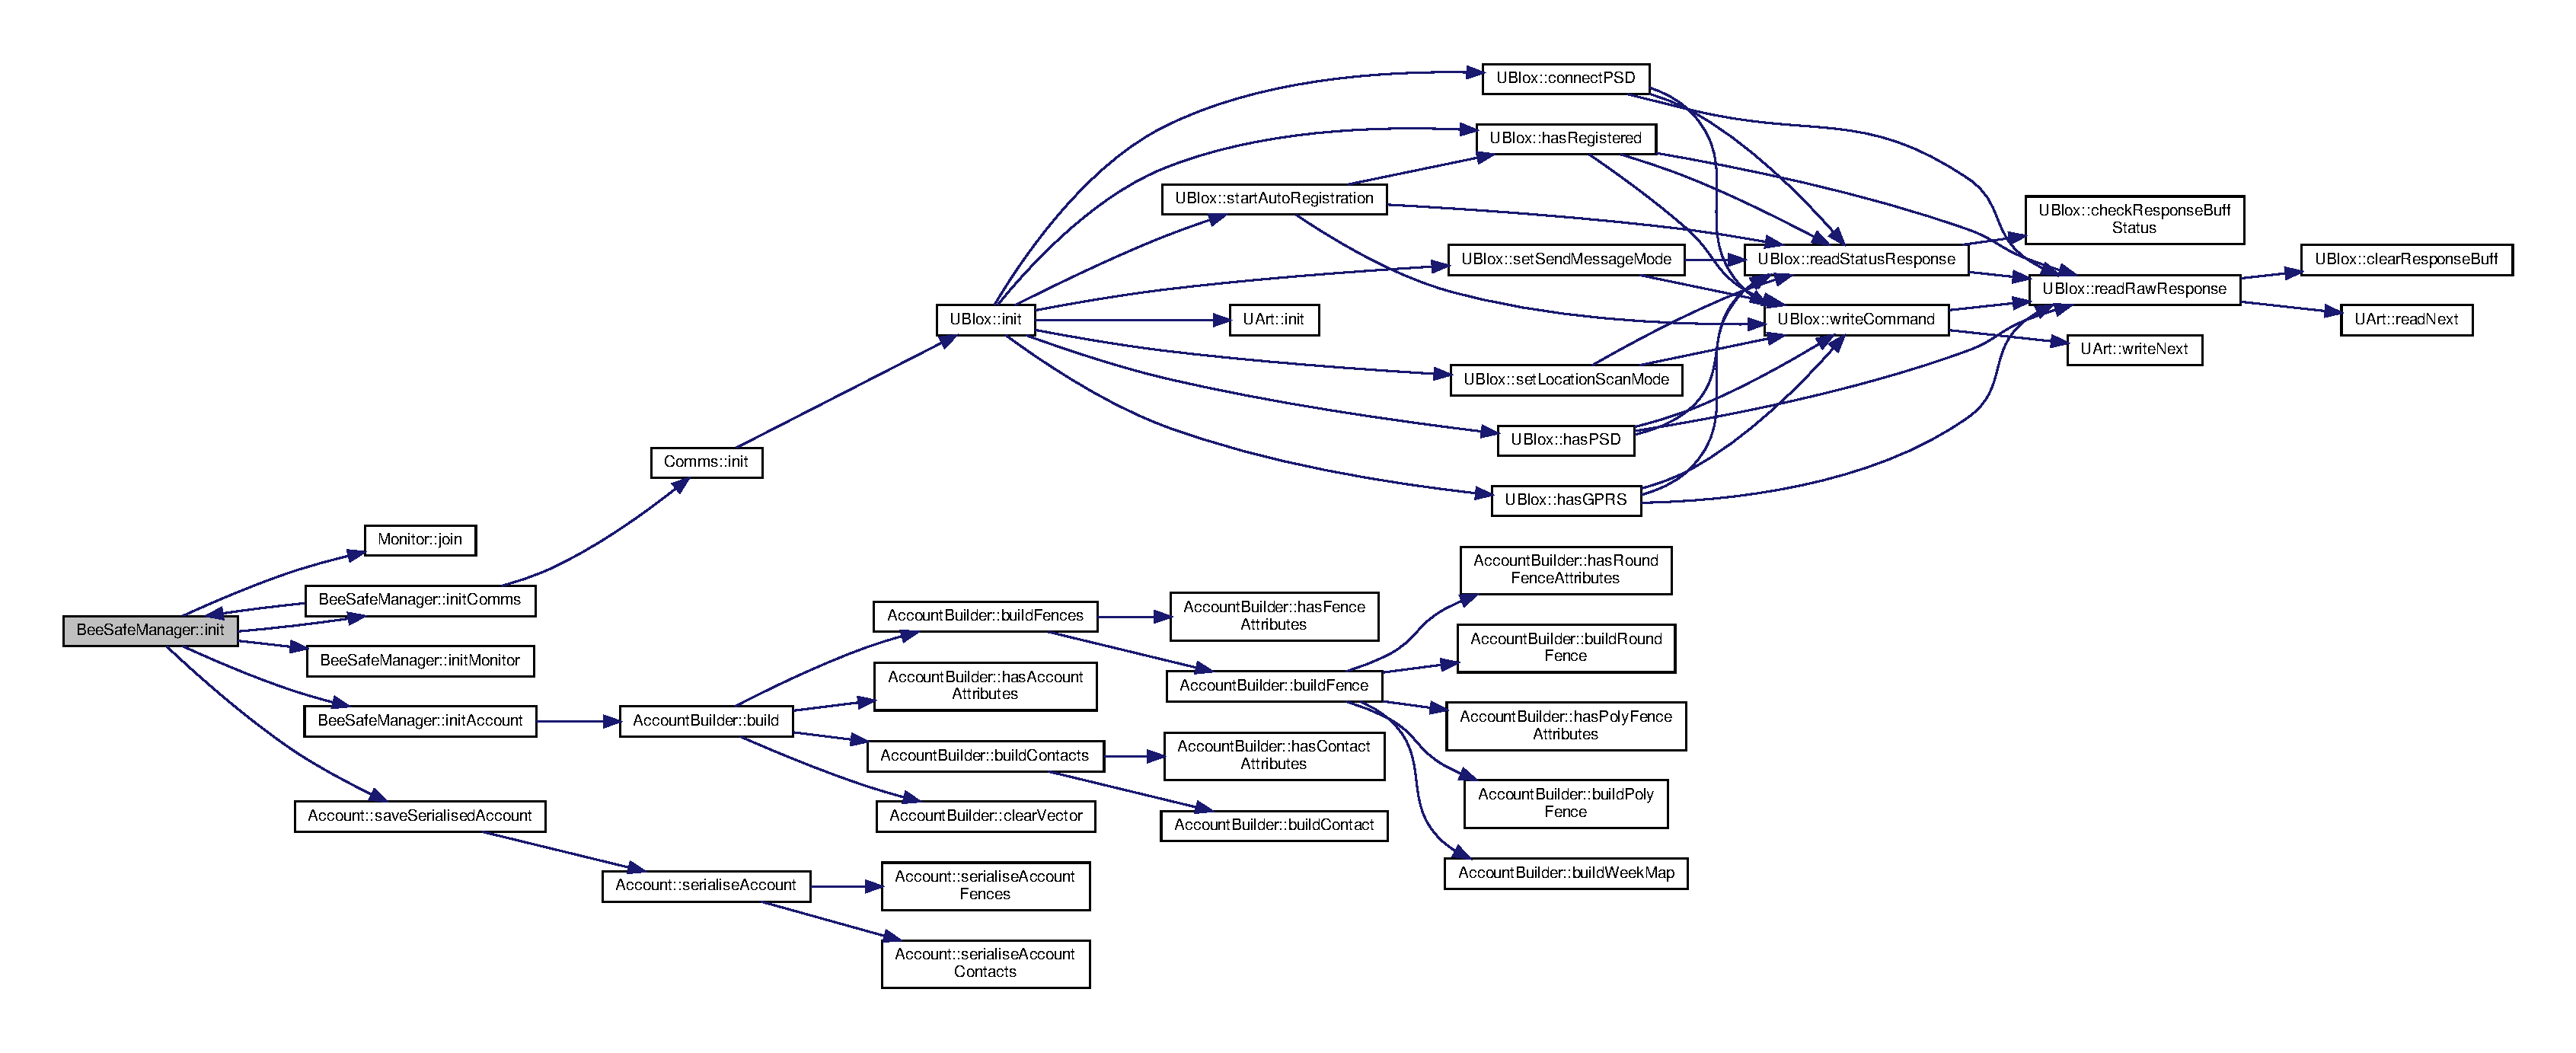
\includegraphics[width=350pt]{d5/d75/class_bee_safe_manager_a2f16b09c454e21c887d14ac5483973cf_cgraph}
\end{center}
\end{figure}
Here is the caller graph for this function\+:\nopagebreak
\begin{figure}[H]
\begin{center}
\leavevmode
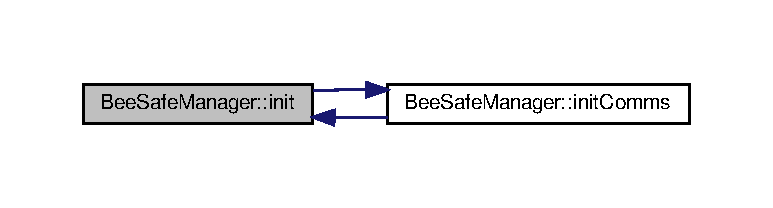
\includegraphics[width=350pt]{d5/d75/class_bee_safe_manager_a2f16b09c454e21c887d14ac5483973cf_icgraph}
\end{center}
\end{figure}
\mbox{\Hypertarget{class_bee_safe_manager_a7395aeacd246ce69c65f255a2eab1d04}\label{class_bee_safe_manager_a7395aeacd246ce69c65f255a2eab1d04}} 
\index{Bee\+Safe\+Manager@{Bee\+Safe\+Manager}!init\+Account@{init\+Account}}
\index{init\+Account@{init\+Account}!Bee\+Safe\+Manager@{Bee\+Safe\+Manager}}
\subsubsection{\texorpdfstring{init\+Account()}{initAccount()}}
{\footnotesize\ttfamily \hyperlink{class_account}{Account} $\ast$ Bee\+Safe\+Manager\+::init\+Account (\begin{DoxyParamCaption}\item[{const char $\ast$}]{path }\end{DoxyParamCaption})\hspace{0.3cm}{\ttfamily [private]}}

Function is responsible for the initialisation / creation (reading) of the local \hyperlink{class_account}{Account} instance.


\begin{DoxyParams}{Parameters}
{\em path} & The file path of the J\+S\+ON file i.\+e. the path to where the Account.\+json file resides. \\
\hline
\end{DoxyParams}
\begin{DoxyReturn}{Returns}
A pointer to an instance of \hyperlink{class_account}{Account} if it was successfully read, parsed and created, nullptr otherwise. 
\end{DoxyReturn}


Definition at line 217 of file Bee\+Safe.\+cpp.


\begin{DoxyCode}
218 \{
219     \textcolor{keywordflow}{try} \{
220         \textcolor{comment}{// Attempt to read the file.}
221         utility::ifstream\_t ifStream;
222         ifStream.open(path);
223         \textcolor{keywordflow}{if} (ifStream.fail()) \{
224             std::cerr << \textcolor{stringliteral}{"Failed to load account file: "} << \hyperlink{_bee_safe_8cpp_aeadb35b2afa47797b56f17423460fad8}{ACCOUNT\_PATH}
225                       << \textcolor{stringliteral}{". Maybe doesn't exist yet?"} << std::endl;
226             \textcolor{keywordflow}{return} \textcolor{keyword}{nullptr};
227         \} \textcolor{keywordflow}{else} \textcolor{keywordflow}{if} (!ifStream.is\_open()) \{
228             std::cerr << \textcolor{stringliteral}{"Failed to open account file: "} << \hyperlink{_bee_safe_8cpp_aeadb35b2afa47797b56f17423460fad8}{ACCOUNT\_PATH} << \textcolor{stringliteral}{"."} << std::endl;
229             \textcolor{keywordflow}{return} \textcolor{keyword}{nullptr};
230         \}
231 
232         \textcolor{comment}{// Stream the file.}
233         utility::stringstream\_t sStream;
234         sStream << ifStream.rdbuf();
235 
236         \textcolor{comment}{// Attempt to build the JSON file.}
237         std::error\_code ec;
238         \hyperlink{class_account_builder}{AccountBuilder} accountBuilder(sStream, ec);
239         \textcolor{keyword}{auto} \hyperlink{class_bee_safe_manager_a52bc9bc8c1ea9608b83d603b142443b0}{account} = accountBuilder.build();
240 
241         \textcolor{keywordflow}{if} (\hyperlink{class_bee_safe_manager_a52bc9bc8c1ea9608b83d603b142443b0}{account} == \textcolor{keyword}{nullptr}) \{
242             std::cerr << \textcolor{stringliteral}{"Failed to build account file: "} << \hyperlink{_bee_safe_8cpp_aeadb35b2afa47797b56f17423460fad8}{ACCOUNT\_PATH}
243                       << \textcolor{stringliteral}{". Error code: "} << ec.value() << \textcolor{stringliteral}{", message: "} << ec.message() << std::endl;
244         \}
245 
246         \textcolor{comment}{// Close the file stream.}
247         ifStream.close();
248 
249         \textcolor{comment}{// Return an account instance, may be null.}
250         \textcolor{keywordflow}{return} \hyperlink{class_bee_safe_manager_a52bc9bc8c1ea9608b83d603b142443b0}{account};
251 
252     \} \textcolor{keywordflow}{catch} (web::json::json\_exception &e) \{
253         std::cerr << e.what() << std::endl;
254         \textcolor{keywordflow}{return} \textcolor{keyword}{nullptr};
255     \}
256 \}
\end{DoxyCode}
Here is the call graph for this function\+:\nopagebreak
\begin{figure}[H]
\begin{center}
\leavevmode
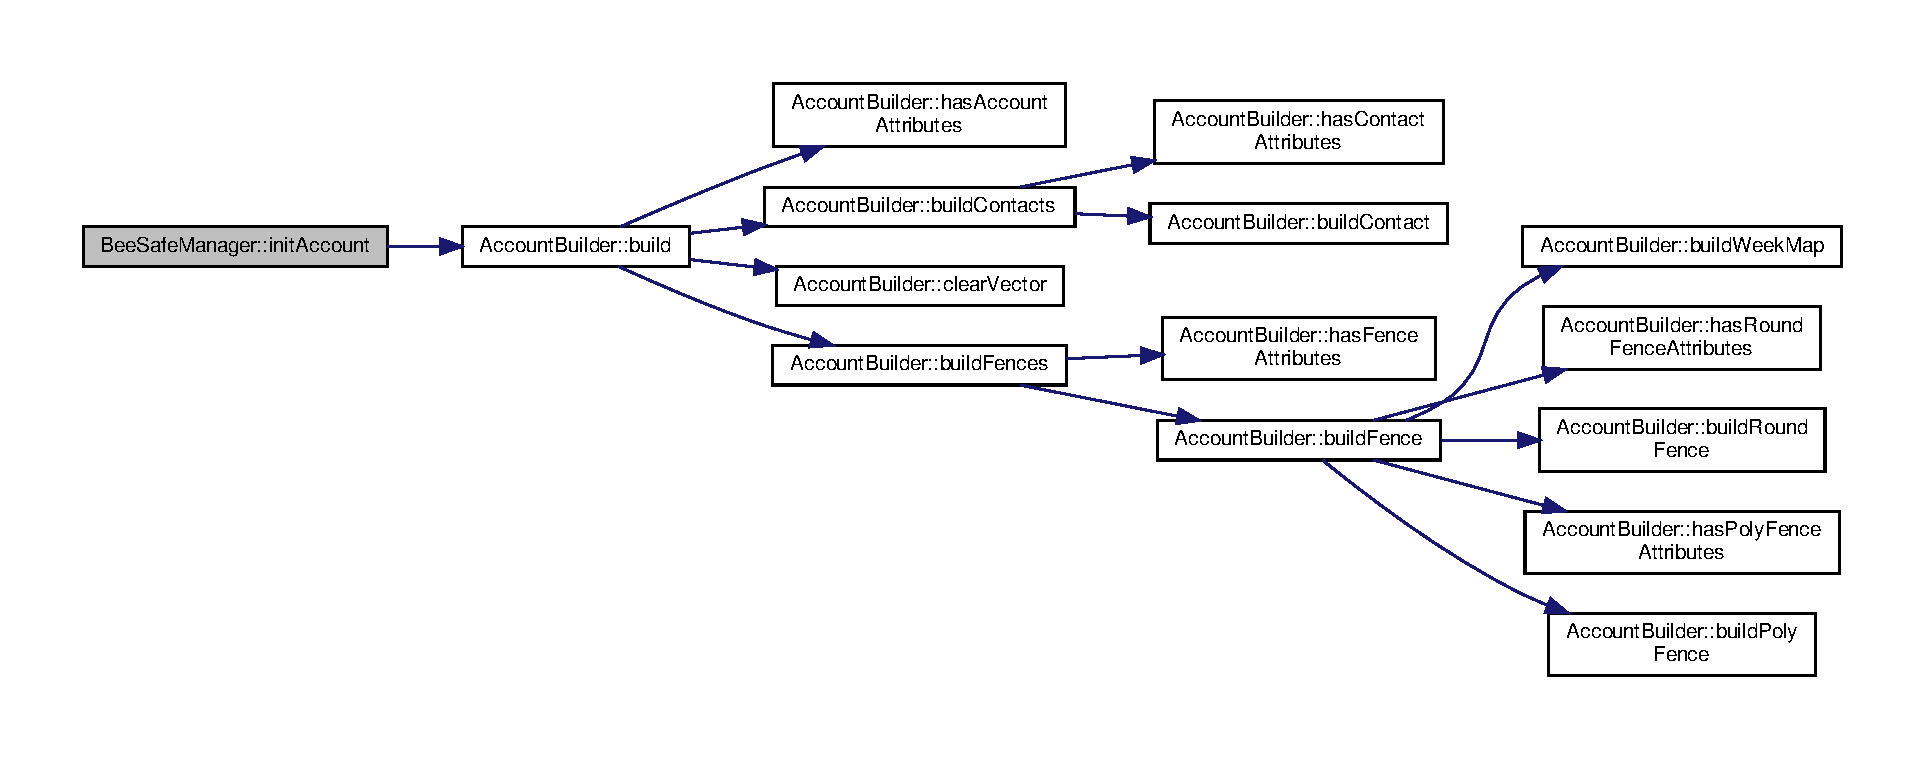
\includegraphics[width=350pt]{d5/d75/class_bee_safe_manager_a7395aeacd246ce69c65f255a2eab1d04_cgraph}
\end{center}
\end{figure}
Here is the caller graph for this function\+:\nopagebreak
\begin{figure}[H]
\begin{center}
\leavevmode
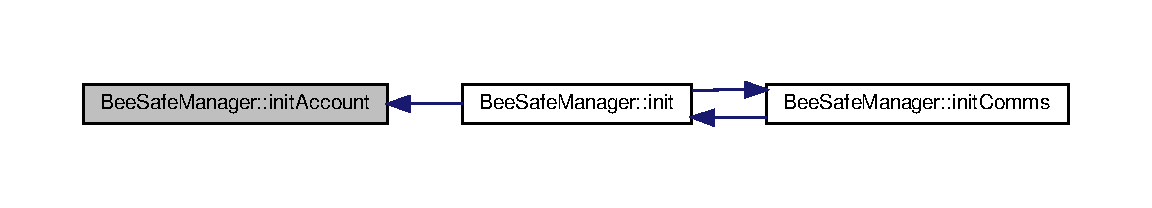
\includegraphics[width=350pt]{d5/d75/class_bee_safe_manager_a7395aeacd246ce69c65f255a2eab1d04_icgraph}
\end{center}
\end{figure}
\mbox{\Hypertarget{class_bee_safe_manager_a28306d7ccf7136a6086d666f4ebb6566}\label{class_bee_safe_manager_a28306d7ccf7136a6086d666f4ebb6566}} 
\index{Bee\+Safe\+Manager@{Bee\+Safe\+Manager}!init\+Comms@{init\+Comms}}
\index{init\+Comms@{init\+Comms}!Bee\+Safe\+Manager@{Bee\+Safe\+Manager}}
\subsubsection{\texorpdfstring{init\+Comms()}{initComms()}}
{\footnotesize\ttfamily \hyperlink{class_comms}{Comms} $\ast$ Bee\+Safe\+Manager\+::init\+Comms (\begin{DoxyParamCaption}{ }\end{DoxyParamCaption})\hspace{0.3cm}{\ttfamily [private]}}

Function is responsible for the creation / initialisation of the \hyperlink{class_comms}{Comms} interface instance.

\begin{DoxyReturn}{Returns}
A pointer to an instance of \hyperlink{class_comms}{Comms} (if successfully initialised / created), nullptr otherwise. 
\end{DoxyReturn}


Definition at line 161 of file Bee\+Safe.\+cpp.


\begin{DoxyCode}
162 \{
163     \textcolor{keyword}{auto} \hyperlink{class_bee_safe_manager_a80b19afbb679d08be14d67a45447f9e1}{comms} = \textcolor{keyword}{new} \hyperlink{class_comms}{Comms}();
164 
165     \textcolor{comment}{// Try numerous times to initialise the comms interface.}
166     \textcolor{keywordtype}{bool} \hyperlink{class_bee_safe_manager_a2f16b09c454e21c887d14ac5483973cf}{init} = \textcolor{keyword}{false};
167     \textcolor{keywordtype}{short} tries = 0;
168     \textcolor{keywordflow}{do} \{
169 
170         \textcolor{comment}{// Attempt to initialise the interface.}
171         tries++;
172         std::cout << \textcolor{stringliteral}{"Comms initialisation attempt "} << tries << \textcolor{stringliteral}{" / "} << 
      \hyperlink{_bee_safe_8cpp_aa5860d80bbb4527d5d2275aacfce65f7}{INIT\_COMMS\_TRIES} << \textcolor{stringliteral}{"..."} <<  std::endl;
173         init = \hyperlink{class_bee_safe_manager_a80b19afbb679d08be14d67a45447f9e1}{comms}->\hyperlink{class_comms_aa0519d3ed2d5bd6aad60101080ac2de7}{init}();
174         \textcolor{keywordflow}{if} (init) \{
175             \textcolor{keywordflow}{break};
176         \} \textcolor{keywordflow}{else} \{
177             std::cerr << \textcolor{stringliteral}{"... comms initialisation attempt "} << tries << \textcolor{stringliteral}{" / "} << 
      \hyperlink{_bee_safe_8cpp_aa5860d80bbb4527d5d2275aacfce65f7}{INIT\_COMMS\_TRIES} << \textcolor{stringliteral}{" failed."} << std::endl;
178         \}
179 
180     \} \textcolor{keywordflow}{while} (tries < \hyperlink{_bee_safe_8cpp_aa5860d80bbb4527d5d2275aacfce65f7}{INIT\_COMMS\_TRIES});
181 
182     \textcolor{comment}{// We failed to initialise the interface.}
183     \textcolor{keywordflow}{if} (!init) \{
184         \textcolor{keyword}{delete} \hyperlink{class_bee_safe_manager_a80b19afbb679d08be14d67a45447f9e1}{comms};
185         \textcolor{keywordflow}{return} \textcolor{keyword}{nullptr};
186     \}
187 
188     \textcolor{comment}{// Successfully return the comms instance.}
189     \textcolor{keywordflow}{return} \hyperlink{class_bee_safe_manager_a80b19afbb679d08be14d67a45447f9e1}{comms};
190 \}
\end{DoxyCode}
Here is the call graph for this function\+:\nopagebreak
\begin{figure}[H]
\begin{center}
\leavevmode
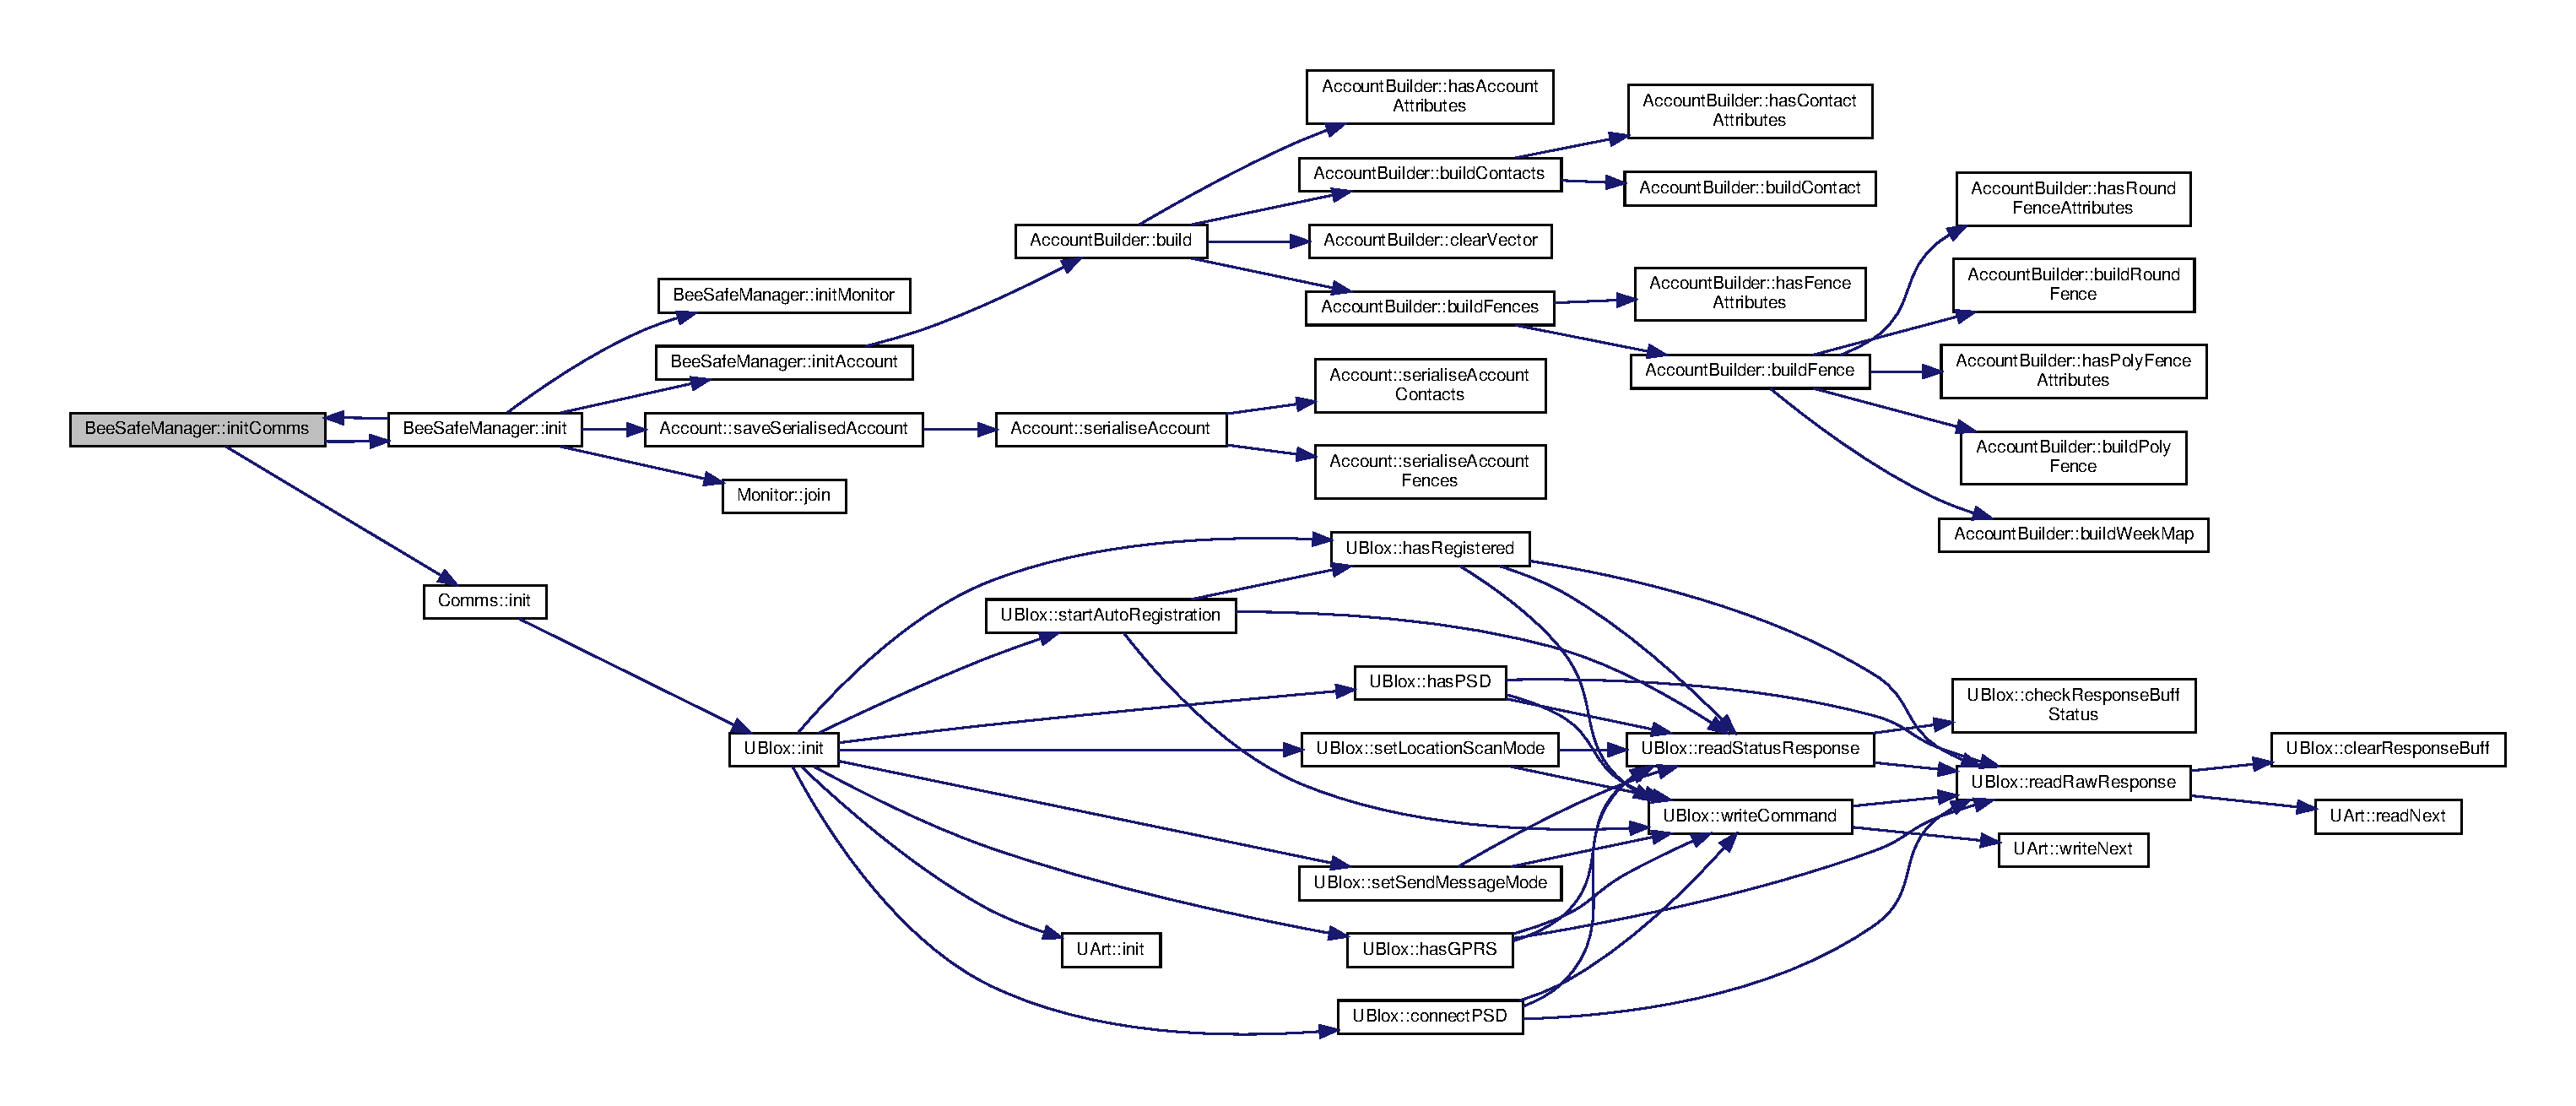
\includegraphics[width=350pt]{d5/d75/class_bee_safe_manager_a28306d7ccf7136a6086d666f4ebb6566_cgraph}
\end{center}
\end{figure}
Here is the caller graph for this function\+:\nopagebreak
\begin{figure}[H]
\begin{center}
\leavevmode
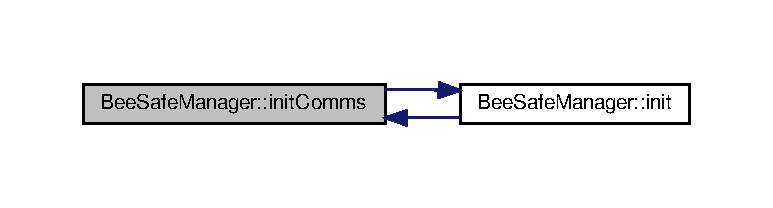
\includegraphics[width=350pt]{d5/d75/class_bee_safe_manager_a28306d7ccf7136a6086d666f4ebb6566_icgraph}
\end{center}
\end{figure}
\mbox{\Hypertarget{class_bee_safe_manager_ad30babe45ead2cb6a5b0559afa5bc5ff}\label{class_bee_safe_manager_ad30babe45ead2cb6a5b0559afa5bc5ff}} 
\index{Bee\+Safe\+Manager@{Bee\+Safe\+Manager}!init\+Monitor@{init\+Monitor}}
\index{init\+Monitor@{init\+Monitor}!Bee\+Safe\+Manager@{Bee\+Safe\+Manager}}
\subsubsection{\texorpdfstring{init\+Monitor()}{initMonitor()}}
{\footnotesize\ttfamily \hyperlink{class_monitor}{Monitor} $\ast$ Bee\+Safe\+Manager\+::init\+Monitor (\begin{DoxyParamCaption}\item[{\hyperlink{class_comms}{Comms} $\ast$}]{comms }\end{DoxyParamCaption})\hspace{0.3cm}{\ttfamily [private]}}

Function is responsible for the creation / initialisation of the \hyperlink{class_monitor}{Monitor} thread instance.


\begin{DoxyParams}{Parameters}
{\em comms} & The communication interface that\textquotesingle{}s to be utilised. \\
\hline
\end{DoxyParams}
\begin{DoxyReturn}{Returns}
A pointer to an instance of \hyperlink{class_monitor}{Monitor} (if successfully initialised / created), nullptr otherwise. 
\end{DoxyReturn}


Definition at line 200 of file Bee\+Safe.\+cpp.


\begin{DoxyCode}
201 \{
202     \textcolor{keywordflow}{if} (comms != \textcolor{keyword}{nullptr}) \{
203         \textcolor{keywordflow}{return} \textcolor{keyword}{new} \hyperlink{class_monitor}{Monitor}(comms);
204     \}
205     \textcolor{keywordflow}{return} \textcolor{keyword}{nullptr};
206 \}
\end{DoxyCode}
Here is the caller graph for this function\+:\nopagebreak
\begin{figure}[H]
\begin{center}
\leavevmode
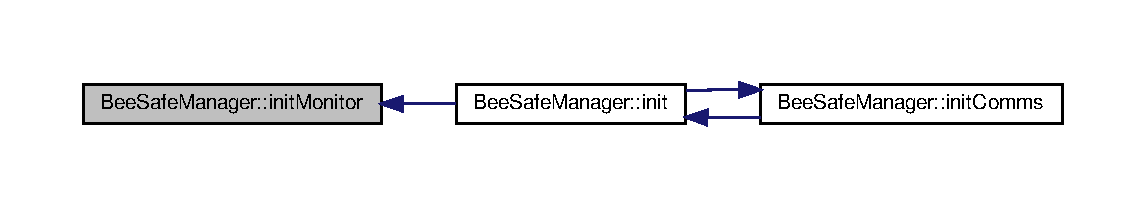
\includegraphics[width=350pt]{d5/d75/class_bee_safe_manager_ad30babe45ead2cb6a5b0559afa5bc5ff_icgraph}
\end{center}
\end{figure}
\mbox{\Hypertarget{class_bee_safe_manager_a7242d89761621de0e09ec9ea360fca27}\label{class_bee_safe_manager_a7242d89761621de0e09ec9ea360fca27}} 
\index{Bee\+Safe\+Manager@{Bee\+Safe\+Manager}!start@{start}}
\index{start@{start}!Bee\+Safe\+Manager@{Bee\+Safe\+Manager}}
\subsubsection{\texorpdfstring{start()}{start()}}
{\footnotesize\ttfamily bool Bee\+Safe\+Manager\+::start (\begin{DoxyParamCaption}{ }\end{DoxyParamCaption})}

A method to start the monitor thread.

\begin{DoxyReturn}{Returns}
True if the thread could be successfully started. 
\end{DoxyReturn}


Definition at line 263 of file Bee\+Safe.\+cpp.


\begin{DoxyCode}
264 \{
265 
266     \textcolor{comment}{// If the account is not null, start the monitor thread.}
267     \textcolor{keywordflow}{if} (\hyperlink{class_bee_safe_manager_a52bc9bc8c1ea9608b83d603b142443b0}{account} != \textcolor{keyword}{nullptr}) \{
268         \textcolor{keywordflow}{if} (!\hyperlink{class_bee_safe_manager_a3b885b4fb364228c914095f2e670f9af}{monitor}->\hyperlink{class_monitor_a71dfa92dfa25ee137f4e3d5e01a8d673}{start}(\hyperlink{class_bee_safe_manager_a52bc9bc8c1ea9608b83d603b142443b0}{account})) \{
269             std::cerr << \textcolor{stringliteral}{"Failed to start the monitor thread."} << std::endl;
270             \textcolor{keywordflow}{return} \textcolor{keyword}{false};
271         \}
272         \hyperlink{class_bee_safe_manager_a3b885b4fb364228c914095f2e670f9af}{monitor}->\hyperlink{class_monitor_a2d2e309666c98333a317c9786f94f6ad}{join}();
273     \}
274 
275     \textcolor{comment}{// TODO: Implement the manager thread for obtaining the account data file.}
276 
277     \textcolor{keywordflow}{return} \textcolor{keyword}{true};
278 \}
\end{DoxyCode}
Here is the call graph for this function\+:\nopagebreak
\begin{figure}[H]
\begin{center}
\leavevmode
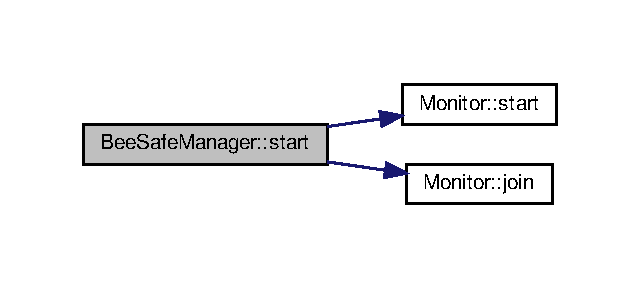
\includegraphics[width=307pt]{d5/d75/class_bee_safe_manager_a7242d89761621de0e09ec9ea360fca27_cgraph}
\end{center}
\end{figure}


\subsection{Member Data Documentation}
\mbox{\Hypertarget{class_bee_safe_manager_a52bc9bc8c1ea9608b83d603b142443b0}\label{class_bee_safe_manager_a52bc9bc8c1ea9608b83d603b142443b0}} 
\index{Bee\+Safe\+Manager@{Bee\+Safe\+Manager}!account@{account}}
\index{account@{account}!Bee\+Safe\+Manager@{Bee\+Safe\+Manager}}
\subsubsection{\texorpdfstring{account}{account}}
{\footnotesize\ttfamily \hyperlink{class_account}{Account}$\ast$ Bee\+Safe\+Manager\+::account\hspace{0.3cm}{\ttfamily [private]}}



Definition at line 72 of file Bee\+Safe.\+h.

\mbox{\Hypertarget{class_bee_safe_manager_a80b19afbb679d08be14d67a45447f9e1}\label{class_bee_safe_manager_a80b19afbb679d08be14d67a45447f9e1}} 
\index{Bee\+Safe\+Manager@{Bee\+Safe\+Manager}!comms@{comms}}
\index{comms@{comms}!Bee\+Safe\+Manager@{Bee\+Safe\+Manager}}
\subsubsection{\texorpdfstring{comms}{comms}}
{\footnotesize\ttfamily \hyperlink{class_comms}{Comms}$\ast$ Bee\+Safe\+Manager\+::comms\hspace{0.3cm}{\ttfamily [private]}}



Definition at line 68 of file Bee\+Safe.\+h.

\mbox{\Hypertarget{class_bee_safe_manager_a3b885b4fb364228c914095f2e670f9af}\label{class_bee_safe_manager_a3b885b4fb364228c914095f2e670f9af}} 
\index{Bee\+Safe\+Manager@{Bee\+Safe\+Manager}!monitor@{monitor}}
\index{monitor@{monitor}!Bee\+Safe\+Manager@{Bee\+Safe\+Manager}}
\subsubsection{\texorpdfstring{monitor}{monitor}}
{\footnotesize\ttfamily \hyperlink{class_monitor}{Monitor}$\ast$ Bee\+Safe\+Manager\+::monitor\hspace{0.3cm}{\ttfamily [private]}}



Definition at line 69 of file Bee\+Safe.\+h.



The documentation for this class was generated from the following files\+:\begin{DoxyCompactItemize}
\item 
software/\+Bee\+Safe\+P\+I/src/\hyperlink{_bee_safe_8h}{Bee\+Safe.\+h}\item 
software/\+Bee\+Safe\+P\+I/src/\hyperlink{_bee_safe_8cpp}{Bee\+Safe.\+cpp}\end{DoxyCompactItemize}

\hypertarget{class_comms}{}\section{Comms Class Reference}
\label{class_comms}\index{Comms@{Comms}}


A high-\/level wrapper for the communication features.  




{\ttfamily \#include $<$Comms.\+h$>$}



Collaboration diagram for Comms\+:\nopagebreak
\begin{figure}[H]
\begin{center}
\leavevmode
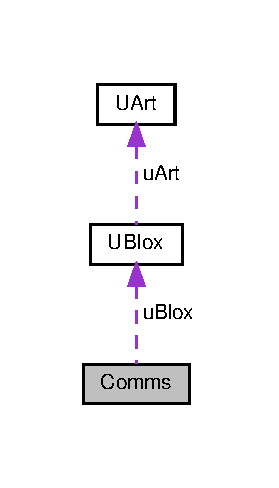
\includegraphics[width=134pt]{d4/d7a/class_comms__coll__graph}
\end{center}
\end{figure}
\subsection*{Public Member Functions}
\begin{DoxyCompactItemize}
\item 
\hyperlink{class_comms_aa3878221ed907d6d6841ee77741c1f49}{Comms} ()
\item 
\hyperlink{class_comms_ad18d3a80a82d18d27b0de3b551e4f5fc}{$\sim$\+Comms} ()
\item 
bool \hyperlink{class_comms_aa0519d3ed2d5bd6aad60101080ac2de7}{init} ()
\item 
const \hyperlink{class_u_blox}{U\+Blox} \& \hyperlink{class_comms_afdd15b4aeca5d91f2f263910c444c957}{get\+U\+Blox} ()
\item 
bool \hyperlink{class_comms_ae1fb7ac11bd07f21134335aec55bd833}{has\+Registered} (bool \&registered)
\item 
bool \hyperlink{class_comms_a583e3d933cca0c1eca9ec77e66bd6b84}{has\+G\+P\+RS} (bool \&attached)
\item 
bool \hyperlink{class_comms_a2c43ce409b48f4d28eefb7934cdd1523}{has\+P\+SD} (bool \&connected)
\item 
bool \hyperlink{class_comms_a9563254514d2f64c0427be2aeaba26d8}{start\+Auto\+Registration} (bool \&registered)
\item 
bool \hyperlink{class_comms_a6d720b51b543ec05b140efdde4cca824}{connect\+P\+SD} (bool \&connected, std\+::string \&urc)
\item 
bool \hyperlink{class_comms_a02eb048febea2d1a39a7fe9e064cf93c}{get\+Model\+Number} (std\+::string \&model\+Number)
\item 
bool \hyperlink{class_comms_ab545396d2360e34fd94e7c3a996e967d}{get\+I\+M\+EI} (std\+::string \&imei\+Number)
\item 
bool \hyperlink{class_comms_ade9963ad1f934a79a6b584dd7abfe515}{get\+Send\+Message\+Mode} (char \&send\+Msg\+Mode)
\item 
bool \hyperlink{class_comms_a1b6f5cafba74fc0e175f057e15656362}{set\+Send\+Message\+Mode} (char send\+Msg\+Mode)
\item 
bool \hyperlink{class_comms_a8f9893e235e62f8fc752f05a06383e68}{get\+Location\+Scan\+Mode} (char \&loc\+Scan\+Mode)
\item 
bool \hyperlink{class_comms_a73c0cd58db7daf118bd0b1726fc9dded}{set\+Location\+Scan\+Mode} (char loc\+Scan\+Mode)
\item 
bool \hyperlink{class_comms_a26030245503e82aa6278e39cd0886c31}{get\+Location} (std\+::pair$<$ double, double $>$ \&lat\+Lng)
\item 
bool \hyperlink{class_comms_a083b399b3115711b1e2d55f800cac58c}{get\+Location} (double \&lat, double \&lng)
\item 
bool \hyperlink{class_comms_a30ab10ea604ab2b169ca66f3f1071c0e}{send\+Message} (\hyperlink{class_contact}{Contact} \&contact, const std\+::string \&message)
\item 
bool \hyperlink{class_comms_ad28b072a0852ac95aa2475324cbfae60}{send\+Message} (const std\+::string \&phone\+Number, const std\+::string \&message)
\end{DoxyCompactItemize}
\subsection*{Private Attributes}
\begin{DoxyCompactItemize}
\item 
\hyperlink{class_u_blox}{U\+Blox} \hyperlink{class_comms_ac64dea134b116147e5441172346dbd6c}{u\+Blox}
\item 
std\+::mutex \hyperlink{class_comms_a21df861b1202573e4cd0cb5666d638fe}{mtx}
\end{DoxyCompactItemize}


\subsection{Detailed Description}
A high-\/level wrapper for the communication features. 

The \hyperlink{class_comms}{Comms} class acts as a high-\/level wrapper over the \hyperlink{class_u_blox}{U\+Blox} class, ensuring concurrency-\/safe access to the hardware. By calling the \hyperlink{class_u_blox}{U\+Blox} commands describing higher level communications functions such as getting a location and sending a text message, and \char`\"{}wrapping it\char`\"{} in a mutex lock it ensures the safe interactions with and operations of the hardware connected to the Raspberry Pi.

\begin{DoxyAuthor}{Author}
Bee\+Safe Team, Team 13
\end{DoxyAuthor}
\begin{DoxyVersion}{Version}
v1.\+0
\end{DoxyVersion}
\begin{DoxyDate}{Date}
2020/04/20
\end{DoxyDate}
\hyperlink{class_contact}{Contact}\+: \href{mailto:beesafe.uofg@gmail.com}{\tt beesafe.\+uofg@gmail.\+com}

Licence\+: M\+IT 

Definition at line 41 of file Comms.\+h.



\subsection{Constructor \& Destructor Documentation}
\mbox{\Hypertarget{class_comms_aa3878221ed907d6d6841ee77741c1f49}\label{class_comms_aa3878221ed907d6d6841ee77741c1f49}} 
\index{Comms@{Comms}!Comms@{Comms}}
\index{Comms@{Comms}!Comms@{Comms}}
\subsubsection{\texorpdfstring{Comms()}{Comms()}}
{\footnotesize\ttfamily Comms\+::\+Comms (\begin{DoxyParamCaption}{ }\end{DoxyParamCaption})\hspace{0.3cm}{\ttfamily [explicit]}, {\ttfamily [default]}}

The \hyperlink{class_comms}{Comms} class constructor. \mbox{\Hypertarget{class_comms_ad18d3a80a82d18d27b0de3b551e4f5fc}\label{class_comms_ad18d3a80a82d18d27b0de3b551e4f5fc}} 
\index{Comms@{Comms}!````~Comms@{$\sim$\+Comms}}
\index{````~Comms@{$\sim$\+Comms}!Comms@{Comms}}
\subsubsection{\texorpdfstring{$\sim$\+Comms()}{~Comms()}}
{\footnotesize\ttfamily Comms\+::$\sim$\+Comms (\begin{DoxyParamCaption}{ }\end{DoxyParamCaption})\hspace{0.3cm}{\ttfamily [default]}}

The \hyperlink{class_comms}{Comms} class destructor. 

\subsection{Member Function Documentation}
\mbox{\Hypertarget{class_comms_a6d720b51b543ec05b140efdde4cca824}\label{class_comms_a6d720b51b543ec05b140efdde4cca824}} 
\index{Comms@{Comms}!connect\+P\+SD@{connect\+P\+SD}}
\index{connect\+P\+SD@{connect\+P\+SD}!Comms@{Comms}}
\subsubsection{\texorpdfstring{connect\+P\+S\+D()}{connectPSD()}}
{\footnotesize\ttfamily bool Comms\+::connect\+P\+SD (\begin{DoxyParamCaption}\item[{bool \&}]{connected,  }\item[{std\+::string \&}]{urc }\end{DoxyParamCaption})}

Attempt to connect to the internet.


\begin{DoxyParams}{Parameters}
{\em connected} & A bool reference into which the result is to be stored i.\+e. whether a connection was successfully established. \\
\hline
{\em urc} & A reference into which additional information is to be stored. \\
\hline
\end{DoxyParams}
\begin{DoxyReturn}{Returns}
True if the command was successfully executed, false otherwise. 
\end{DoxyReturn}


Definition at line 154 of file Comms.\+cpp.


\begin{DoxyCode}
155 \{
156     \textcolor{comment}{// Lock the comms interface and connect.}
157     \hyperlink{class_comms_a21df861b1202573e4cd0cb5666d638fe}{mtx}.lock();
158     \textcolor{keywordtype}{bool} rc = \hyperlink{class_comms_ac64dea134b116147e5441172346dbd6c}{uBlox}.\hyperlink{class_u_blox_ac250bd4aea14e09b3a2595c2b8eda18a}{connectPSD}(connected, urc);
159     \hyperlink{class_comms_a21df861b1202573e4cd0cb5666d638fe}{mtx}.unlock();
160 
161     \textcolor{comment}{// Return the state of the command.}
162     \textcolor{keywordflow}{return} rc;
163 \}
\end{DoxyCode}
Here is the call graph for this function\+:\nopagebreak
\begin{figure}[H]
\begin{center}
\leavevmode
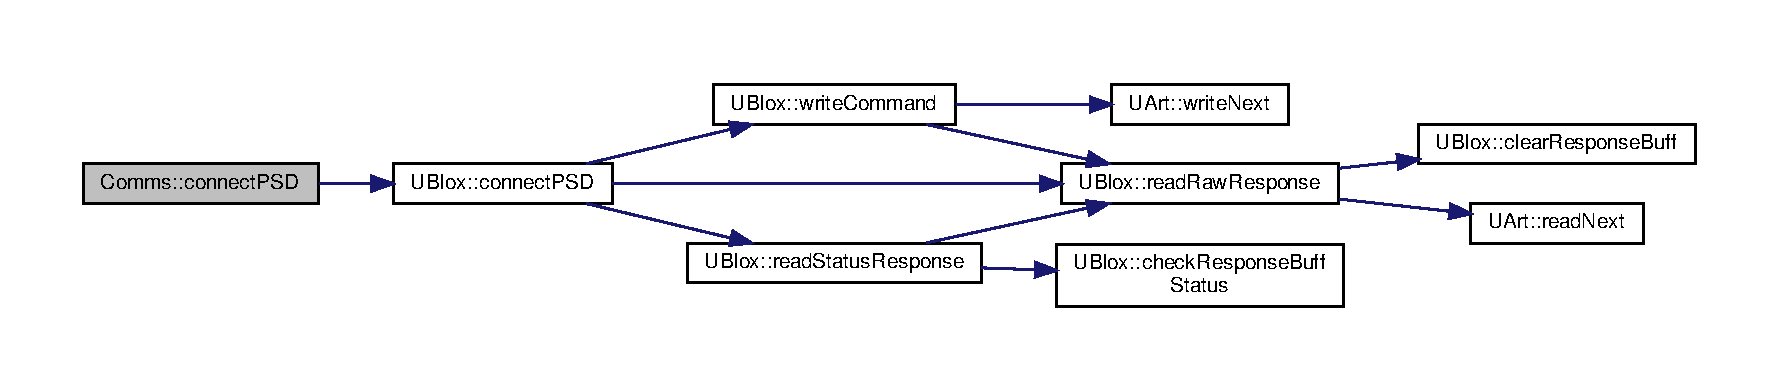
\includegraphics[width=350pt]{d8/dcc/class_comms_a6d720b51b543ec05b140efdde4cca824_cgraph}
\end{center}
\end{figure}
Here is the caller graph for this function\+:\nopagebreak
\begin{figure}[H]
\begin{center}
\leavevmode
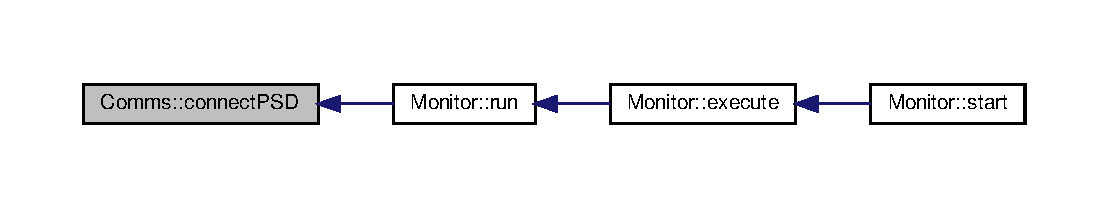
\includegraphics[width=350pt]{d8/dcc/class_comms_a6d720b51b543ec05b140efdde4cca824_icgraph}
\end{center}
\end{figure}
\mbox{\Hypertarget{class_comms_ab545396d2360e34fd94e7c3a996e967d}\label{class_comms_ab545396d2360e34fd94e7c3a996e967d}} 
\index{Comms@{Comms}!get\+I\+M\+EI@{get\+I\+M\+EI}}
\index{get\+I\+M\+EI@{get\+I\+M\+EI}!Comms@{Comms}}
\subsubsection{\texorpdfstring{get\+I\+M\+E\+I()}{getIMEI()}}
{\footnotesize\ttfamily bool Comms\+::get\+I\+M\+EI (\begin{DoxyParamCaption}\item[{std\+::string \&}]{imei\+Number }\end{DoxyParamCaption})}

Get the I\+M\+EI number associated with the device.


\begin{DoxyParams}{Parameters}
{\em imei\+Number} & The string reference into which the result i.\+e. imei will be stored. \\
\hline
\end{DoxyParams}
\begin{DoxyReturn}{Returns}
True if the function successfully obtained the result, false otherwise. 
\end{DoxyReturn}


Definition at line 192 of file Comms.\+cpp.


\begin{DoxyCode}
193 \{
194     \textcolor{comment}{// Locks the comms interface and get the imeiNumber number.}
195     \hyperlink{class_comms_a21df861b1202573e4cd0cb5666d638fe}{mtx}.lock();
196     \textcolor{keywordtype}{bool} rc = \hyperlink{class_comms_ac64dea134b116147e5441172346dbd6c}{uBlox}.\hyperlink{class_u_blox_ade30654ab2eab43d322dc6b516866401}{getIMEI}(imeiNumber);
197     \hyperlink{class_comms_a21df861b1202573e4cd0cb5666d638fe}{mtx}.unlock();
198 
199     \textcolor{comment}{// Return the result of the function.}
200     \textcolor{keywordflow}{return} rc;
201 \}
\end{DoxyCode}
Here is the call graph for this function\+:\nopagebreak
\begin{figure}[H]
\begin{center}
\leavevmode
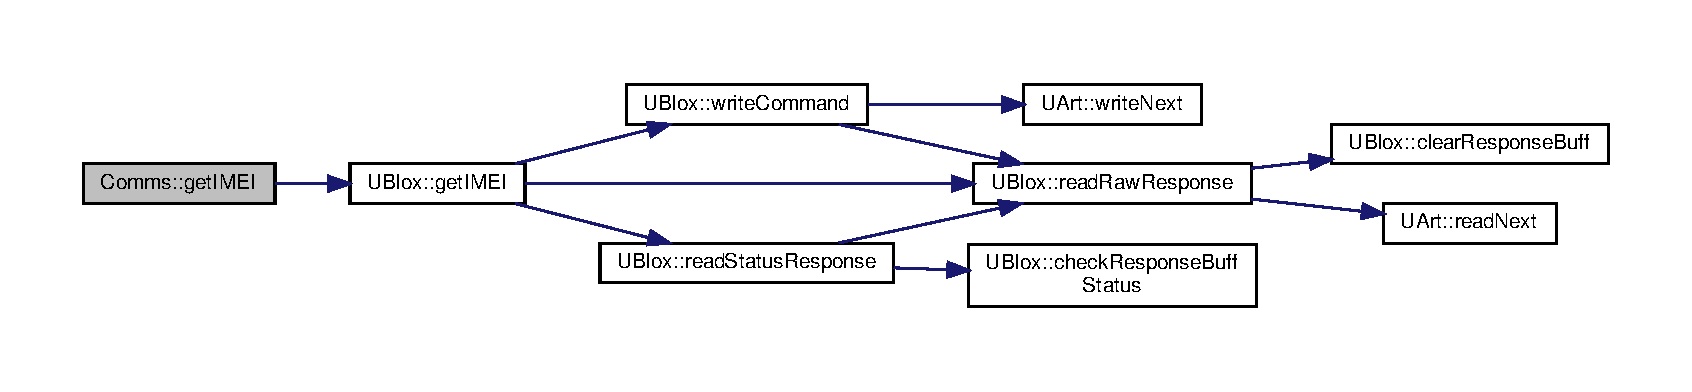
\includegraphics[width=350pt]{d8/dcc/class_comms_ab545396d2360e34fd94e7c3a996e967d_cgraph}
\end{center}
\end{figure}
\mbox{\Hypertarget{class_comms_a26030245503e82aa6278e39cd0886c31}\label{class_comms_a26030245503e82aa6278e39cd0886c31}} 
\index{Comms@{Comms}!get\+Location@{get\+Location}}
\index{get\+Location@{get\+Location}!Comms@{Comms}}
\subsubsection{\texorpdfstring{get\+Location()}{getLocation()}\hspace{0.1cm}{\footnotesize\ttfamily [1/2]}}
{\footnotesize\ttfamily bool Comms\+::get\+Location (\begin{DoxyParamCaption}\item[{std\+::pair$<$ double, double $>$ \&}]{lat\+Lng }\end{DoxyParamCaption})}

Get the location of the device on which the code is being run.

Note, the function delegates the locking to the \hyperlink{class_comms_a083b399b3115711b1e2d55f800cac58c}{get\+Location(double \&lat, double \&lng)}.


\begin{DoxyParams}{Parameters}
{\em lat\+Lng} & The pair structure into which the result is to be placed. \textquotesingle{}first\textquotesingle{} represents the latitude whereas \textquotesingle{}second\textquotesingle{} represents the latitude. \\
\hline
\end{DoxyParams}
\begin{DoxyReturn}{Returns}
True if the function returned successfully, false otherwise. 
\end{DoxyReturn}


Definition at line 291 of file Comms.\+cpp.


\begin{DoxyCode}
292 \{
293     \textcolor{keywordflow}{return} \hyperlink{class_comms_a26030245503e82aa6278e39cd0886c31}{getLocation}(latLng.first, latLng.second);
294 \}
\end{DoxyCode}
Here is the caller graph for this function\+:\nopagebreak
\begin{figure}[H]
\begin{center}
\leavevmode
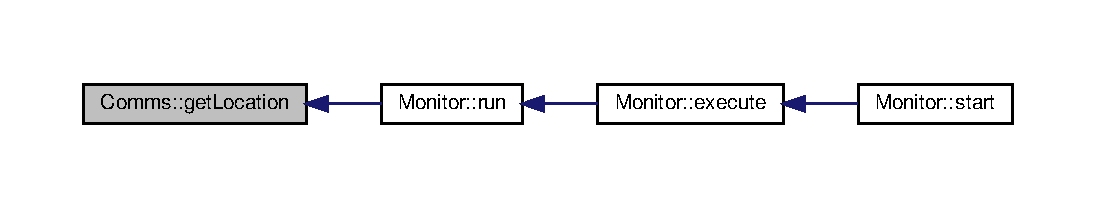
\includegraphics[width=350pt]{d8/dcc/class_comms_a26030245503e82aa6278e39cd0886c31_icgraph}
\end{center}
\end{figure}
\mbox{\Hypertarget{class_comms_a083b399b3115711b1e2d55f800cac58c}\label{class_comms_a083b399b3115711b1e2d55f800cac58c}} 
\index{Comms@{Comms}!get\+Location@{get\+Location}}
\index{get\+Location@{get\+Location}!Comms@{Comms}}
\subsubsection{\texorpdfstring{get\+Location()}{getLocation()}\hspace{0.1cm}{\footnotesize\ttfamily [2/2]}}
{\footnotesize\ttfamily bool Comms\+::get\+Location (\begin{DoxyParamCaption}\item[{double \&}]{lat,  }\item[{double \&}]{lng }\end{DoxyParamCaption})}

Get the location of the device on which the code is being run.


\begin{DoxyParams}{Parameters}
{\em lat} & The geo-\/location latitude. \\
\hline
{\em lng} & The geo-\/location longitude. \\
\hline
\end{DoxyParams}
\begin{DoxyReturn}{Returns}
True if the function returned successfully, false otherwise. 
\end{DoxyReturn}


Definition at line 303 of file Comms.\+cpp.


\begin{DoxyCode}
304 \{
305     \textcolor{comment}{// Lock the comms interface and get the latitude and longitude.}
306     \hyperlink{class_comms_a21df861b1202573e4cd0cb5666d638fe}{mtx}.lock();
307     \textcolor{keywordtype}{bool} rc = \hyperlink{class_comms_ac64dea134b116147e5441172346dbd6c}{uBlox}.\hyperlink{class_u_blox_a2443d175bbf55a4f4facc5d8a99d2723}{getLocation}(lat, lng);
308     \hyperlink{class_comms_a21df861b1202573e4cd0cb5666d638fe}{mtx}.unlock();
309 
310     \textcolor{comment}{// Return the result of the operation.}
311     \textcolor{keywordflow}{return} rc;
312 \}
\end{DoxyCode}
Here is the call graph for this function\+:\nopagebreak
\begin{figure}[H]
\begin{center}
\leavevmode
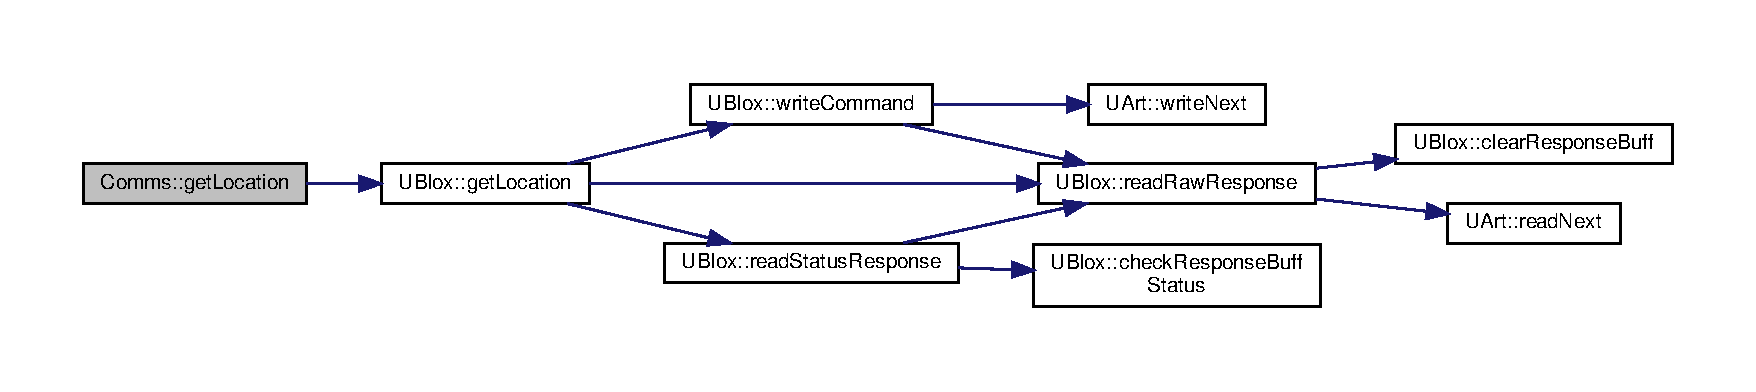
\includegraphics[width=350pt]{d8/dcc/class_comms_a083b399b3115711b1e2d55f800cac58c_cgraph}
\end{center}
\end{figure}
\mbox{\Hypertarget{class_comms_a8f9893e235e62f8fc752f05a06383e68}\label{class_comms_a8f9893e235e62f8fc752f05a06383e68}} 
\index{Comms@{Comms}!get\+Location\+Scan\+Mode@{get\+Location\+Scan\+Mode}}
\index{get\+Location\+Scan\+Mode@{get\+Location\+Scan\+Mode}!Comms@{Comms}}
\subsubsection{\texorpdfstring{get\+Location\+Scan\+Mode()}{getLocationScanMode()}}
{\footnotesize\ttfamily bool Comms\+::get\+Location\+Scan\+Mode (\begin{DoxyParamCaption}\item[{char \&}]{loc\+Scan\+Mode }\end{DoxyParamCaption})}

Get the Cell\+Locate location scan mode that\textquotesingle{}s utilised for obtaining the latitude and longitude coordinates.


\begin{DoxyParams}{Parameters}
{\em loc\+Scan\+Mode} & The char reference into which the mode (L\+O\+C\+\_\+\+S\+C\+A\+N\+\_\+\+M\+O\+D\+E\+\_\+\+N\+O\+R\+M\+AL or L\+O\+C\+\_\+\+S\+C\+A\+N\+\_\+\+M\+O\+D\+E\+\_\+\+D\+E\+EP) is to be stored. \\
\hline
\end{DoxyParams}
\begin{DoxyReturn}{Returns}
True if the function successfully returned a result, false otherwise. 
\end{DoxyReturn}


Definition at line 249 of file Comms.\+cpp.


\begin{DoxyCode}
250 \{
251     \textcolor{comment}{// Lock the comms and get the location scan mode.}
252     \hyperlink{class_comms_a21df861b1202573e4cd0cb5666d638fe}{mtx}.lock();
253     \textcolor{keywordtype}{bool} rc = \hyperlink{class_comms_ac64dea134b116147e5441172346dbd6c}{uBlox}.\hyperlink{class_u_blox_a398db4cdc2d5356fb86b3cd1021bad1b}{getLocationScanMode}(locScanMode);
254     \hyperlink{class_comms_a21df861b1202573e4cd0cb5666d638fe}{mtx}.unlock();
255 
256     \textcolor{comment}{// Return the state of the function.}
257     \textcolor{keywordflow}{return} rc;
258 \}
\end{DoxyCode}
Here is the call graph for this function\+:\nopagebreak
\begin{figure}[H]
\begin{center}
\leavevmode
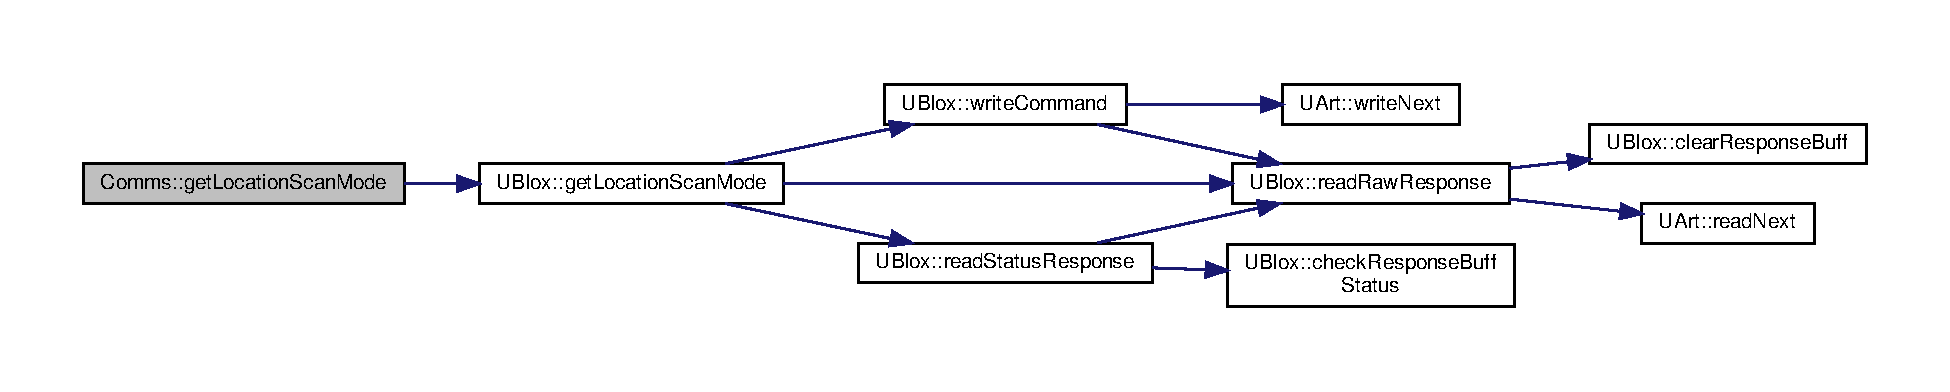
\includegraphics[width=350pt]{d8/dcc/class_comms_a8f9893e235e62f8fc752f05a06383e68_cgraph}
\end{center}
\end{figure}
\mbox{\Hypertarget{class_comms_a02eb048febea2d1a39a7fe9e064cf93c}\label{class_comms_a02eb048febea2d1a39a7fe9e064cf93c}} 
\index{Comms@{Comms}!get\+Model\+Number@{get\+Model\+Number}}
\index{get\+Model\+Number@{get\+Model\+Number}!Comms@{Comms}}
\subsubsection{\texorpdfstring{get\+Model\+Number()}{getModelNumber()}}
{\footnotesize\ttfamily bool Comms\+::get\+Model\+Number (\begin{DoxyParamCaption}\item[{std\+::string \&}]{model\+Number }\end{DoxyParamCaption})}

Get the model number of the u-\/\+Blox device.


\begin{DoxyParams}{Parameters}
{\em model\+Number} & The string reference into which the result i.\+e. model number will be stored. \\
\hline
\end{DoxyParams}
\begin{DoxyReturn}{Returns}
True if the function successfully obtained the result, false otherwise. 
\end{DoxyReturn}


Definition at line 173 of file Comms.\+cpp.


\begin{DoxyCode}
174 \{
175     \textcolor{comment}{// Locks the comms interface and get the model number.}
176     \hyperlink{class_comms_a21df861b1202573e4cd0cb5666d638fe}{mtx}.lock();
177     \textcolor{keywordtype}{bool} rc = \hyperlink{class_comms_ac64dea134b116147e5441172346dbd6c}{uBlox}.\hyperlink{class_u_blox_ab9b9a03e10360c931686c1fe04af078d}{getModelNumber}(modelNumber);
178     \hyperlink{class_comms_a21df861b1202573e4cd0cb5666d638fe}{mtx}.unlock();
179 
180     \textcolor{comment}{// Return the result of the function.}
181     \textcolor{keywordflow}{return} rc;
182 \}
\end{DoxyCode}
Here is the call graph for this function\+:\nopagebreak
\begin{figure}[H]
\begin{center}
\leavevmode
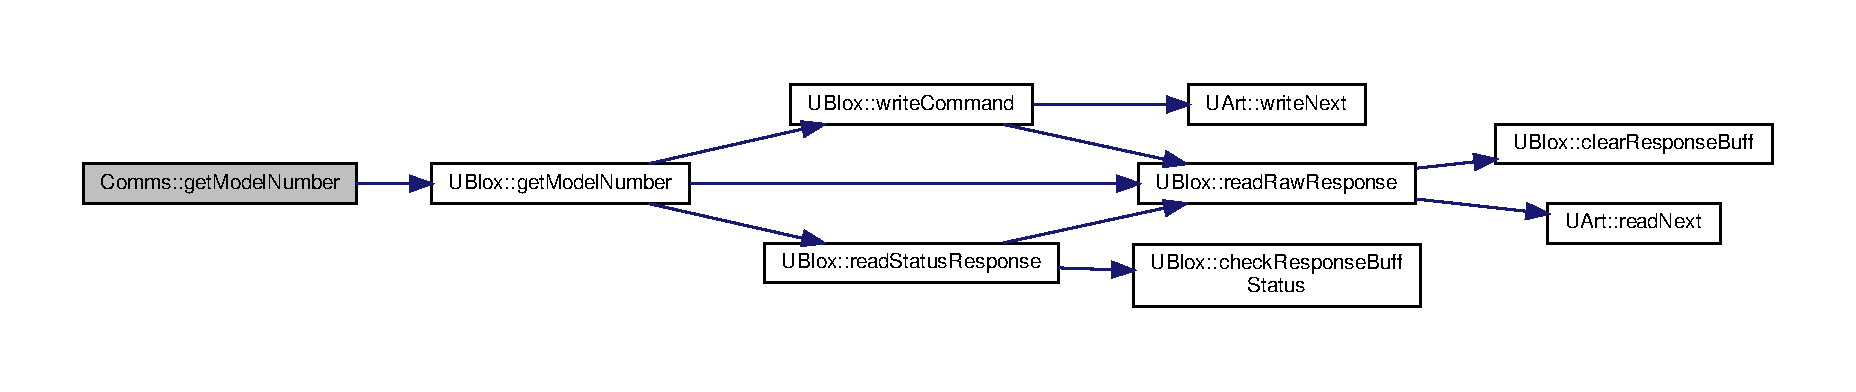
\includegraphics[width=350pt]{d8/dcc/class_comms_a02eb048febea2d1a39a7fe9e064cf93c_cgraph}
\end{center}
\end{figure}
\mbox{\Hypertarget{class_comms_ade9963ad1f934a79a6b584dd7abfe515}\label{class_comms_ade9963ad1f934a79a6b584dd7abfe515}} 
\index{Comms@{Comms}!get\+Send\+Message\+Mode@{get\+Send\+Message\+Mode}}
\index{get\+Send\+Message\+Mode@{get\+Send\+Message\+Mode}!Comms@{Comms}}
\subsubsection{\texorpdfstring{get\+Send\+Message\+Mode()}{getSendMessageMode()}}
{\footnotesize\ttfamily bool Comms\+::get\+Send\+Message\+Mode (\begin{DoxyParamCaption}\item[{char \&}]{send\+Msg\+Mode }\end{DoxyParamCaption})}

Get the send message mode utilised by the device to send text messages.


\begin{DoxyParams}{Parameters}
{\em send\+Msg\+Mode} & The char reference into which the mode (S\+E\+N\+D\+\_\+\+T\+E\+X\+T\+\_\+\+M\+O\+D\+E\+\_\+\+P\+DU or S\+E\+N\+D\+\_\+\+T\+E\+X\+T\+\_\+\+M\+O\+D\+E\+\_\+\+T\+E\+XT) is to be stored. \\
\hline
\end{DoxyParams}
\begin{DoxyReturn}{Returns}
True if the function successfully obtained the send message mode false otherwise. 
\end{DoxyReturn}


Definition at line 211 of file Comms.\+cpp.


\begin{DoxyCode}
212 \{
213     \textcolor{comment}{// Lock the comms interface and get the message mode.}
214     \hyperlink{class_comms_a21df861b1202573e4cd0cb5666d638fe}{mtx}.lock();
215     \textcolor{keywordtype}{bool} rc = \hyperlink{class_comms_ac64dea134b116147e5441172346dbd6c}{uBlox}.\hyperlink{class_u_blox_aee30d82dcf52335d19f77e766db78ab4}{getSendMessageMode}(sendMsgMode);
216     \hyperlink{class_comms_a21df861b1202573e4cd0cb5666d638fe}{mtx}.unlock();
217 
218     \textcolor{comment}{// Return the state of the function.}
219     \textcolor{keywordflow}{return} rc;
220 \}
\end{DoxyCode}
Here is the call graph for this function\+:\nopagebreak
\begin{figure}[H]
\begin{center}
\leavevmode
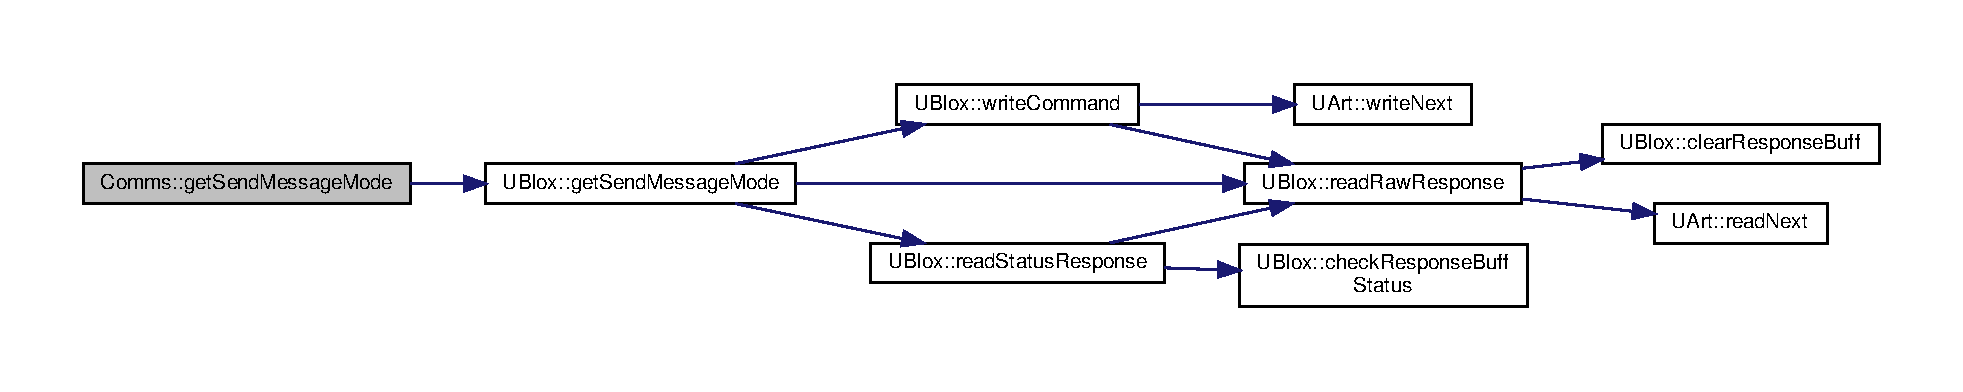
\includegraphics[width=350pt]{d8/dcc/class_comms_ade9963ad1f934a79a6b584dd7abfe515_cgraph}
\end{center}
\end{figure}
\mbox{\Hypertarget{class_comms_afdd15b4aeca5d91f2f263910c444c957}\label{class_comms_afdd15b4aeca5d91f2f263910c444c957}} 
\index{Comms@{Comms}!get\+U\+Blox@{get\+U\+Blox}}
\index{get\+U\+Blox@{get\+U\+Blox}!Comms@{Comms}}
\subsubsection{\texorpdfstring{get\+U\+Blox()}{getUBlox()}}
{\footnotesize\ttfamily const \hyperlink{class_u_blox}{U\+Blox} \& Comms\+::get\+U\+Blox (\begin{DoxyParamCaption}{ }\end{DoxyParamCaption})}

Get the u-\/blox device that the comms interface utilises for communication.

Invocation of the function does not lock the comms interface. Moreover, there are no locks associated with underlying structures. Thus, this function (and the returned instance of \hyperlink{class_u_blox}{U\+Blox}) should be used with extreme care.

\begin{DoxyReturn}{Returns}
An instance of the \hyperlink{class_u_blox}{U\+Blox} device utilised to communicate via the U\+A\+RT interface. 
\end{DoxyReturn}


Definition at line 66 of file Comms.\+cpp.


\begin{DoxyCode}
67 \{
68     \textcolor{keywordflow}{return} \hyperlink{class_comms_ac64dea134b116147e5441172346dbd6c}{uBlox};
69 \}
\end{DoxyCode}
\mbox{\Hypertarget{class_comms_a583e3d933cca0c1eca9ec77e66bd6b84}\label{class_comms_a583e3d933cca0c1eca9ec77e66bd6b84}} 
\index{Comms@{Comms}!has\+G\+P\+RS@{has\+G\+P\+RS}}
\index{has\+G\+P\+RS@{has\+G\+P\+RS}!Comms@{Comms}}
\subsubsection{\texorpdfstring{has\+G\+P\+R\+S()}{hasGPRS()}}
{\footnotesize\ttfamily bool Comms\+::has\+G\+P\+RS (\begin{DoxyParamCaption}\item[{bool \&}]{attached }\end{DoxyParamCaption})}

Determines whether or not the G\+P\+RS is attached to the device.


\begin{DoxyParams}{Parameters}
{\em attached} & The bool reference into which the result of whether or not G\+P\+RS is attached will be stored. \\
\hline
\end{DoxyParams}
\begin{DoxyReturn}{Returns}
True if the function successfully obtained the result, false otherwise. 
\end{DoxyReturn}


Definition at line 97 of file Comms.\+cpp.


\begin{DoxyCode}
98 \{
99     \textcolor{comment}{// Lock the comms interface and check if GPRS is attached.}
100     \hyperlink{class_comms_a21df861b1202573e4cd0cb5666d638fe}{mtx}.lock();
101     \textcolor{keywordtype}{bool} rc = \hyperlink{class_comms_ac64dea134b116147e5441172346dbd6c}{uBlox}.\hyperlink{class_u_blox_a4f5a31b4ddda664b255ce3f63e9ffac7}{hasGPRS}(attached);
102     \hyperlink{class_comms_a21df861b1202573e4cd0cb5666d638fe}{mtx}.unlock();
103 
104     \textcolor{comment}{// Return the result of the function.}
105     \textcolor{keywordflow}{return} rc;
106 \}
\end{DoxyCode}
Here is the call graph for this function\+:\nopagebreak
\begin{figure}[H]
\begin{center}
\leavevmode
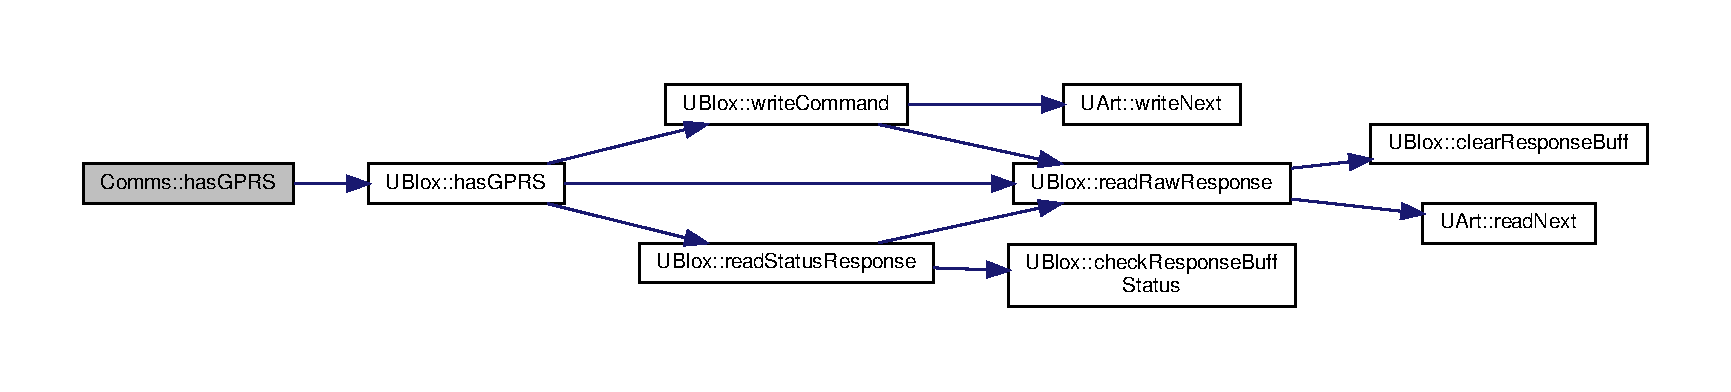
\includegraphics[width=350pt]{d8/dcc/class_comms_a583e3d933cca0c1eca9ec77e66bd6b84_cgraph}
\end{center}
\end{figure}
\mbox{\Hypertarget{class_comms_a2c43ce409b48f4d28eefb7934cdd1523}\label{class_comms_a2c43ce409b48f4d28eefb7934cdd1523}} 
\index{Comms@{Comms}!has\+P\+SD@{has\+P\+SD}}
\index{has\+P\+SD@{has\+P\+SD}!Comms@{Comms}}
\subsubsection{\texorpdfstring{has\+P\+S\+D()}{hasPSD()}}
{\footnotesize\ttfamily bool Comms\+::has\+P\+SD (\begin{DoxyParamCaption}\item[{bool \&}]{connected }\end{DoxyParamCaption})}

Determines whether or not the P\+SD (internet) is connected.


\begin{DoxyParams}{Parameters}
{\em connected} & The bool reference into which the result of whether or not the P\+SD (internet) is connected will be stored. \\
\hline
\end{DoxyParams}
\begin{DoxyReturn}{Returns}
True if the function successfully obtained the result, false otherwise. 
\end{DoxyReturn}


Definition at line 116 of file Comms.\+cpp.


\begin{DoxyCode}
117 \{
118     \textcolor{comment}{// Lock the comms interface and check if PSD connected.}
119     \hyperlink{class_comms_a21df861b1202573e4cd0cb5666d638fe}{mtx}.lock();
120     \textcolor{keywordtype}{bool} rc = \hyperlink{class_comms_ac64dea134b116147e5441172346dbd6c}{uBlox}.\hyperlink{class_u_blox_ae49b51a602a327b5eff5b04d2ccaec20}{hasPSD}(connected);
121     \hyperlink{class_comms_a21df861b1202573e4cd0cb5666d638fe}{mtx}.unlock();
122 
123     \textcolor{comment}{// Return the result of the function.}
124     \textcolor{keywordflow}{return} rc;
125 \}
\end{DoxyCode}
Here is the call graph for this function\+:\nopagebreak
\begin{figure}[H]
\begin{center}
\leavevmode
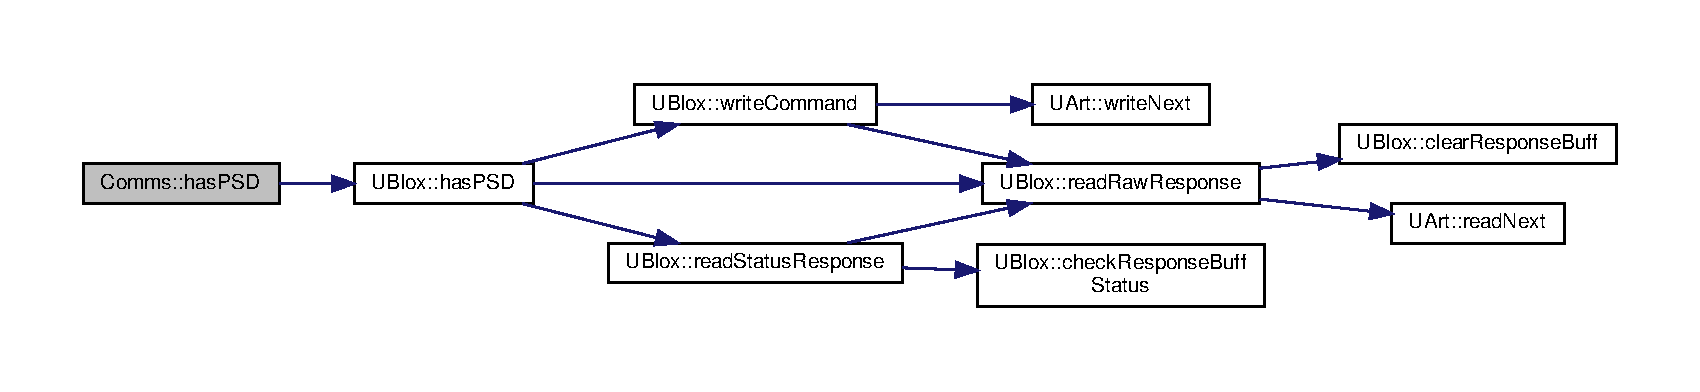
\includegraphics[width=350pt]{d8/dcc/class_comms_a2c43ce409b48f4d28eefb7934cdd1523_cgraph}
\end{center}
\end{figure}
Here is the caller graph for this function\+:\nopagebreak
\begin{figure}[H]
\begin{center}
\leavevmode
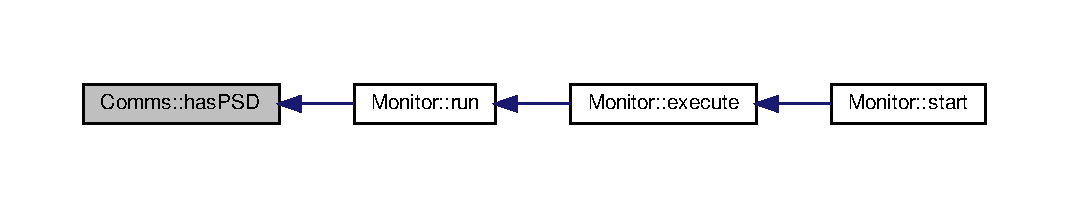
\includegraphics[width=350pt]{d8/dcc/class_comms_a2c43ce409b48f4d28eefb7934cdd1523_icgraph}
\end{center}
\end{figure}
\mbox{\Hypertarget{class_comms_ae1fb7ac11bd07f21134335aec55bd833}\label{class_comms_ae1fb7ac11bd07f21134335aec55bd833}} 
\index{Comms@{Comms}!has\+Registered@{has\+Registered}}
\index{has\+Registered@{has\+Registered}!Comms@{Comms}}
\subsubsection{\texorpdfstring{has\+Registered()}{hasRegistered()}}
{\footnotesize\ttfamily bool Comms\+::has\+Registered (\begin{DoxyParamCaption}\item[{bool \&}]{registered }\end{DoxyParamCaption})}

Checks whether or not the device sim is registered with a network.


\begin{DoxyParams}{Parameters}
{\em registered} & The bool reference into which the result is to be stored. \\
\hline
\end{DoxyParams}
\begin{DoxyReturn}{Returns}
True if the device successfully returned the result, false otherwise. 
\end{DoxyReturn}


Definition at line 78 of file Comms.\+cpp.


\begin{DoxyCode}
79 \{
80     \textcolor{comment}{// Lock comms and check if the device is registered to the network.}
81     \hyperlink{class_comms_a21df861b1202573e4cd0cb5666d638fe}{mtx}.lock();
82     \textcolor{keywordtype}{bool} rc = \hyperlink{class_comms_ac64dea134b116147e5441172346dbd6c}{uBlox}.\hyperlink{class_u_blox_a1889c2b9bb6087bc939bd2a27b68623b}{hasRegistered}(registered);
83     \hyperlink{class_comms_a21df861b1202573e4cd0cb5666d638fe}{mtx}.unlock();
84 
85     \textcolor{comment}{// Return the state of the command.}
86     \textcolor{keywordflow}{return} rc;
87 \}
\end{DoxyCode}
Here is the call graph for this function\+:\nopagebreak
\begin{figure}[H]
\begin{center}
\leavevmode
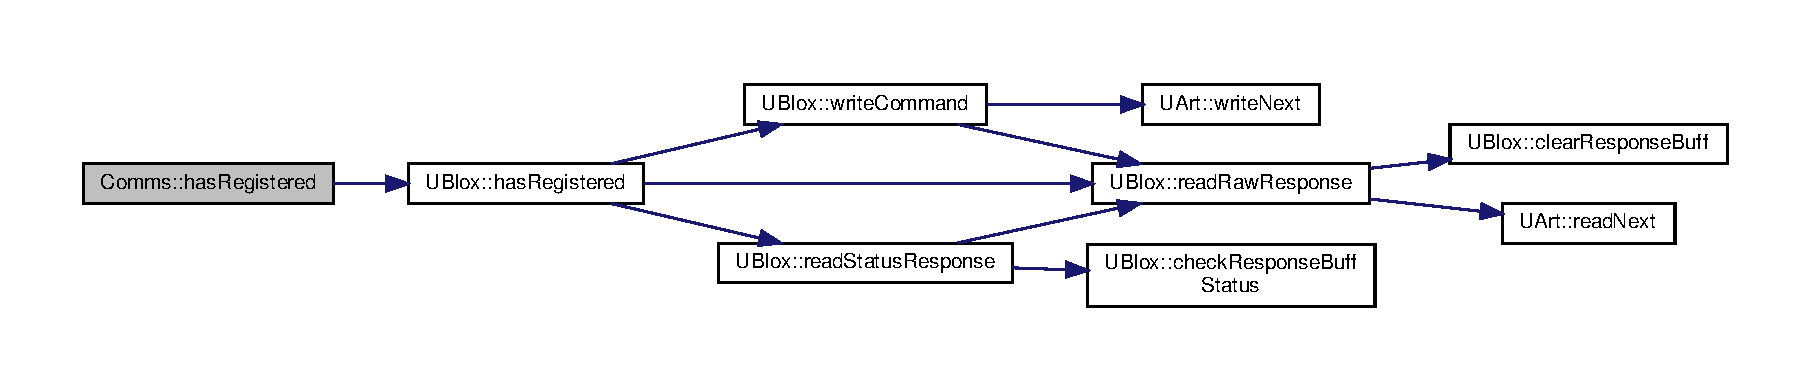
\includegraphics[width=350pt]{d8/dcc/class_comms_ae1fb7ac11bd07f21134335aec55bd833_cgraph}
\end{center}
\end{figure}
\mbox{\Hypertarget{class_comms_aa0519d3ed2d5bd6aad60101080ac2de7}\label{class_comms_aa0519d3ed2d5bd6aad60101080ac2de7}} 
\index{Comms@{Comms}!init@{init}}
\index{init@{init}!Comms@{Comms}}
\subsubsection{\texorpdfstring{init()}{init()}}
{\footnotesize\ttfamily bool Comms\+::init (\begin{DoxyParamCaption}{ }\end{DoxyParamCaption})}

Initialise or re-\/initialise the comms interface. Any prior non-\/default configurations will be reset.

\begin{DoxyReturn}{Returns}
True if the comms interface was successfully initialised, false otherwise. 
\end{DoxyReturn}


Definition at line 43 of file Comms.\+cpp.


\begin{DoxyCode}
44 \{
45     \textcolor{comment}{// Lock and initialise the comms interface.}
46     \hyperlink{class_comms_a21df861b1202573e4cd0cb5666d638fe}{mtx}.lock();
47     \textcolor{keywordtype}{bool} initialised = \hyperlink{class_comms_ac64dea134b116147e5441172346dbd6c}{uBlox}.\hyperlink{class_u_blox_a34c2f507ff3bbd21b9aea788a015527a}{init}();
48     \hyperlink{class_comms_a21df861b1202573e4cd0cb5666d638fe}{mtx}.unlock();
49 
50     \textcolor{comment}{// Whether or not the comms was successfully initialised.}
51     \textcolor{keywordflow}{return} initialised;
52 \}
\end{DoxyCode}
Here is the call graph for this function\+:\nopagebreak
\begin{figure}[H]
\begin{center}
\leavevmode
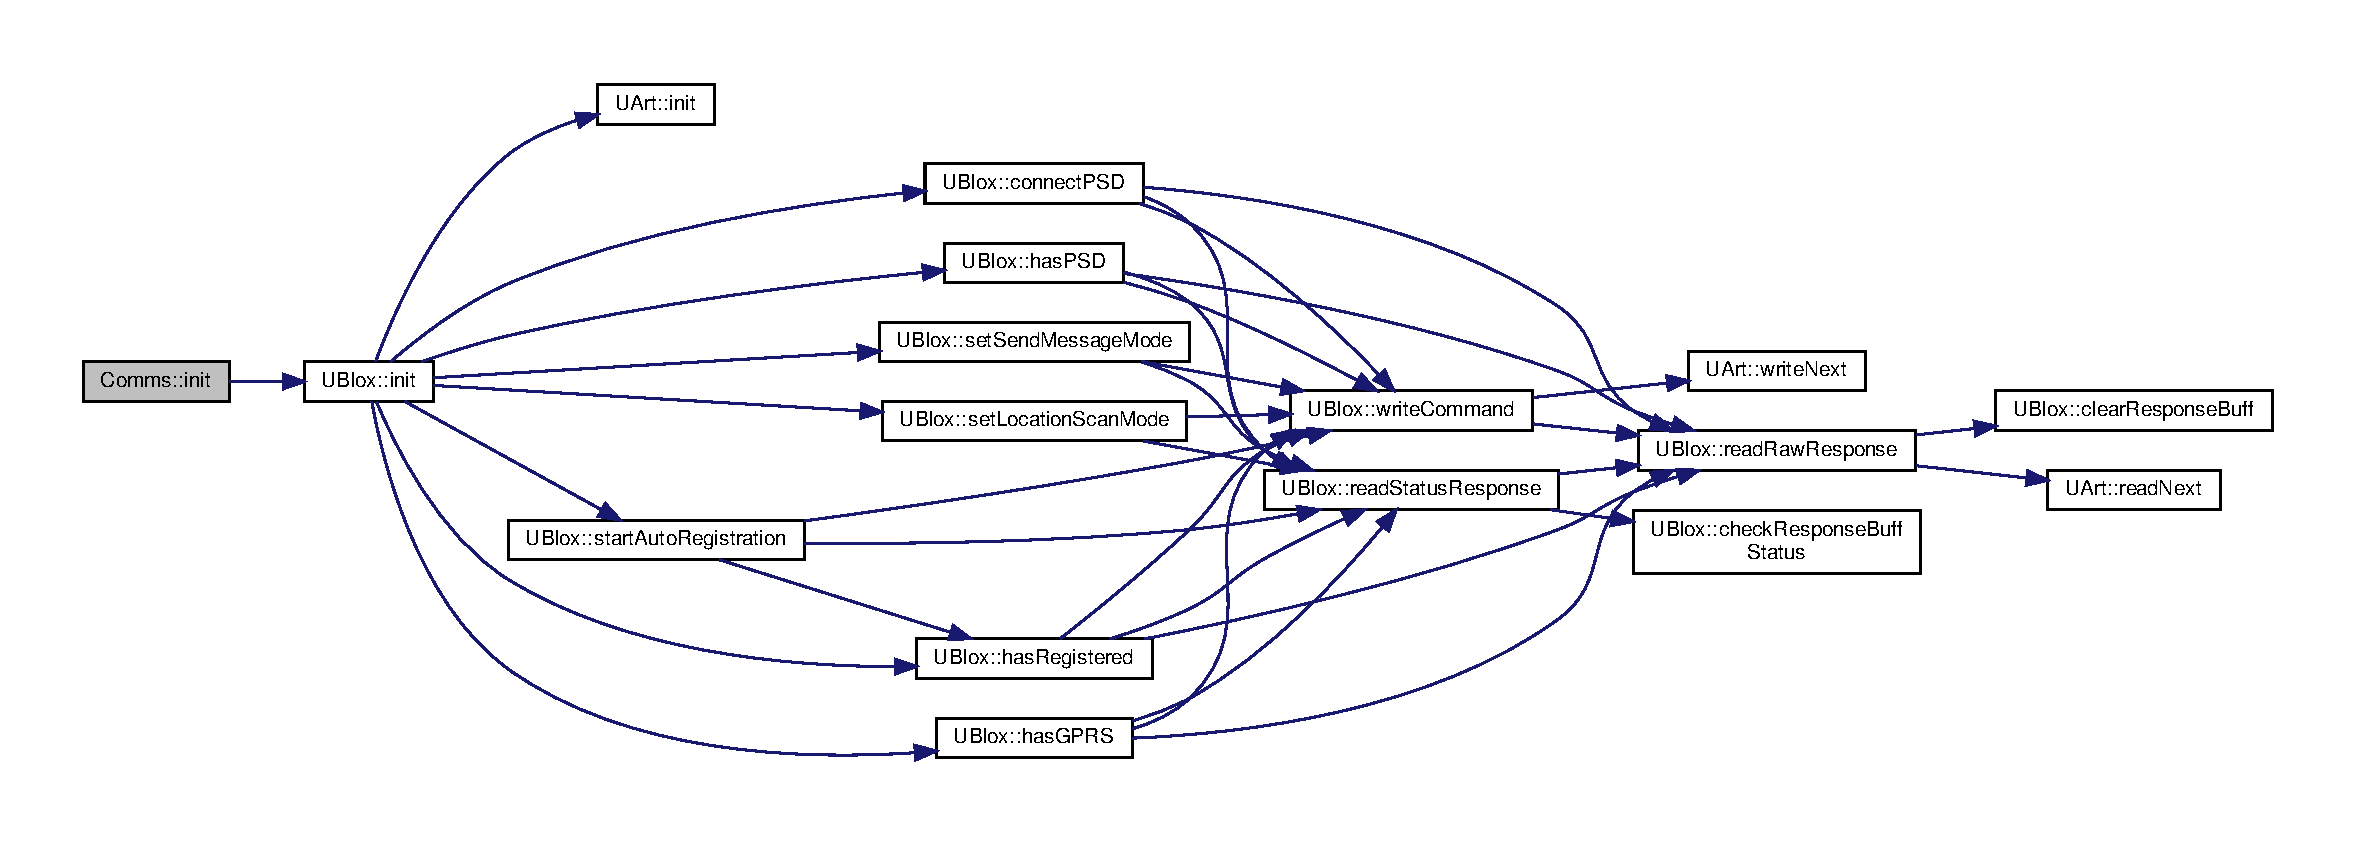
\includegraphics[width=350pt]{d8/dcc/class_comms_aa0519d3ed2d5bd6aad60101080ac2de7_cgraph}
\end{center}
\end{figure}
Here is the caller graph for this function\+:\nopagebreak
\begin{figure}[H]
\begin{center}
\leavevmode
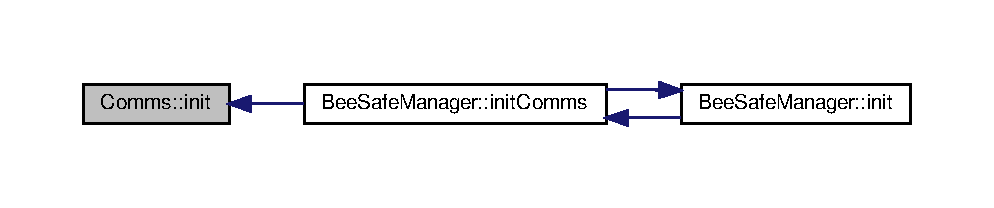
\includegraphics[width=350pt]{d8/dcc/class_comms_aa0519d3ed2d5bd6aad60101080ac2de7_icgraph}
\end{center}
\end{figure}
\mbox{\Hypertarget{class_comms_a30ab10ea604ab2b169ca66f3f1071c0e}\label{class_comms_a30ab10ea604ab2b169ca66f3f1071c0e}} 
\index{Comms@{Comms}!send\+Message@{send\+Message}}
\index{send\+Message@{send\+Message}!Comms@{Comms}}
\subsubsection{\texorpdfstring{send\+Message()}{sendMessage()}\hspace{0.1cm}{\footnotesize\ttfamily [1/2]}}
{\footnotesize\ttfamily bool Comms\+::send\+Message (\begin{DoxyParamCaption}\item[{\hyperlink{class_contact}{Contact} \&}]{contact,  }\item[{const std\+::string \&}]{message }\end{DoxyParamCaption})}

Send a message to a contacts phone number via the \hyperlink{class_u_blox}{U\+Blox} device.

Note, the function delegates the locking to the send\+Message(string \&phone\+Number, string \&message) function.


\begin{DoxyParams}{Parameters}
{\em contact} & The contact (phone number) to which the message will be sent. \\
\hline
{\em message} & The message contents that are to be sent. \\
\hline
\end{DoxyParams}
\begin{DoxyReturn}{Returns}
True if the message was successfully sent, false otherwise. 
\end{DoxyReturn}


Definition at line 324 of file Comms.\+cpp.


\begin{DoxyCode}
325 \{
326    \textcolor{keywordflow}{return} \hyperlink{class_comms_a30ab10ea604ab2b169ca66f3f1071c0e}{sendMessage}(contact.\hyperlink{class_contact_a612095b153e05538c32400c4c44cb1aa}{getNumber}(), message);
327 \}
\end{DoxyCode}
Here is the call graph for this function\+:\nopagebreak
\begin{figure}[H]
\begin{center}
\leavevmode
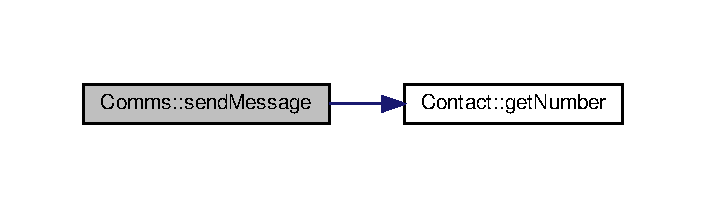
\includegraphics[width=339pt]{d8/dcc/class_comms_a30ab10ea604ab2b169ca66f3f1071c0e_cgraph}
\end{center}
\end{figure}
Here is the caller graph for this function\+:\nopagebreak
\begin{figure}[H]
\begin{center}
\leavevmode
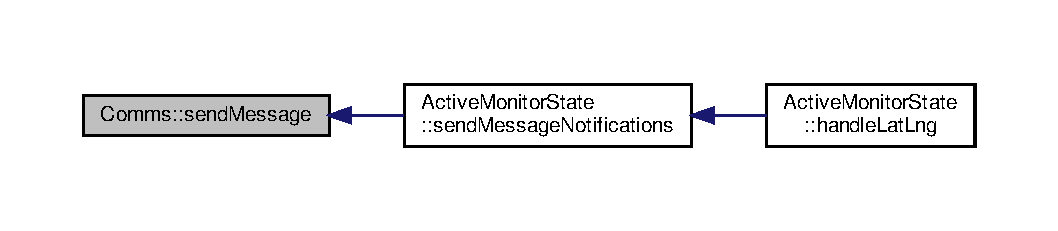
\includegraphics[width=350pt]{d8/dcc/class_comms_a30ab10ea604ab2b169ca66f3f1071c0e_icgraph}
\end{center}
\end{figure}
\mbox{\Hypertarget{class_comms_ad28b072a0852ac95aa2475324cbfae60}\label{class_comms_ad28b072a0852ac95aa2475324cbfae60}} 
\index{Comms@{Comms}!send\+Message@{send\+Message}}
\index{send\+Message@{send\+Message}!Comms@{Comms}}
\subsubsection{\texorpdfstring{send\+Message()}{sendMessage()}\hspace{0.1cm}{\footnotesize\ttfamily [2/2]}}
{\footnotesize\ttfamily bool Comms\+::send\+Message (\begin{DoxyParamCaption}\item[{const std\+::string \&}]{phone\+Number,  }\item[{const std\+::string \&}]{message }\end{DoxyParamCaption})}

Send a message to a mobile phone via the \hyperlink{class_u_blox}{U\+Blox} device.


\begin{DoxyParams}{Parameters}
{\em phone\+Number} & The phone number to which the message will be sent. \\
\hline
{\em message} & The message contents that are to be sent. \\
\hline
\end{DoxyParams}
\begin{DoxyReturn}{Returns}
True if the message was sent successfully, false otherwise. 
\end{DoxyReturn}


Definition at line 336 of file Comms.\+cpp.


\begin{DoxyCode}
337 \{
338     \textcolor{comment}{// Lock the comms interface and set a message.}
339     \hyperlink{class_comms_a21df861b1202573e4cd0cb5666d638fe}{mtx}.lock();
340     \textcolor{keywordtype}{bool} rc = \hyperlink{class_comms_ac64dea134b116147e5441172346dbd6c}{uBlox}.\hyperlink{class_u_blox_a946f2903bb01a62cd5bdef423eaa9750}{sendMessage}(phoneNumber, message);
341     \hyperlink{class_comms_a21df861b1202573e4cd0cb5666d638fe}{mtx}.unlock();
342 
343     \textcolor{comment}{// Return the result of the operation.}
344     \textcolor{keywordflow}{return} rc;
345 \}
\end{DoxyCode}
Here is the call graph for this function\+:\nopagebreak
\begin{figure}[H]
\begin{center}
\leavevmode
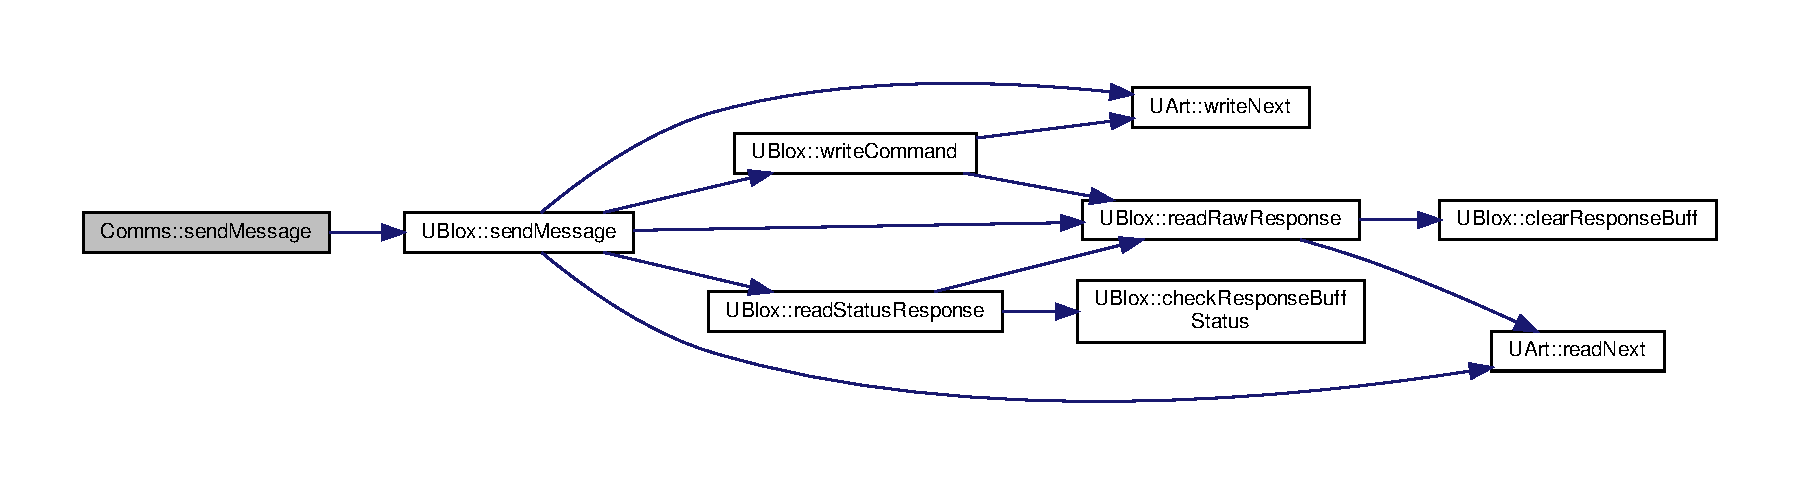
\includegraphics[width=350pt]{d8/dcc/class_comms_ad28b072a0852ac95aa2475324cbfae60_cgraph}
\end{center}
\end{figure}
\mbox{\Hypertarget{class_comms_a73c0cd58db7daf118bd0b1726fc9dded}\label{class_comms_a73c0cd58db7daf118bd0b1726fc9dded}} 
\index{Comms@{Comms}!set\+Location\+Scan\+Mode@{set\+Location\+Scan\+Mode}}
\index{set\+Location\+Scan\+Mode@{set\+Location\+Scan\+Mode}!Comms@{Comms}}
\subsubsection{\texorpdfstring{set\+Location\+Scan\+Mode()}{setLocationScanMode()}}
{\footnotesize\ttfamily bool Comms\+::set\+Location\+Scan\+Mode (\begin{DoxyParamCaption}\item[{char}]{loc\+Scan\+Mode }\end{DoxyParamCaption})}

Set the Cell\+Locate location scan mode that is to be used for obtaining the latitude and longitude coordinates.


\begin{DoxyParams}{Parameters}
{\em loc\+Scan\+Mode} & The mode (L\+O\+C\+\_\+\+S\+C\+A\+N\+\_\+\+M\+O\+D\+E\+\_\+\+N\+O\+R\+M\+AL or L\+O\+C\+\_\+\+S\+C\+A\+N\+\_\+\+M\+O\+D\+E\+\_\+\+D\+E\+EP) that is to be used for obtaining the location. \\
\hline
\end{DoxyParams}
\begin{DoxyReturn}{Returns}
True if the function successfully set the location scan mode, false otherwise. 
\end{DoxyReturn}


Definition at line 269 of file Comms.\+cpp.


\begin{DoxyCode}
270 \{
271     \textcolor{comment}{// Lock comms and set the location scan mode.}
272     \hyperlink{class_comms_a21df861b1202573e4cd0cb5666d638fe}{mtx}.lock();
273     \textcolor{keywordtype}{bool} rc = \hyperlink{class_comms_ac64dea134b116147e5441172346dbd6c}{uBlox}.\hyperlink{class_u_blox_aabed44fd41e16c9d1a8daba80f3bef06}{setLocationScanMode}(locScanMode);
274     \hyperlink{class_comms_a21df861b1202573e4cd0cb5666d638fe}{mtx}.unlock();
275 
276     \textcolor{comment}{// Return the state of the function.}
277     \textcolor{keywordflow}{return} rc;
278 \}
\end{DoxyCode}
Here is the call graph for this function\+:\nopagebreak
\begin{figure}[H]
\begin{center}
\leavevmode
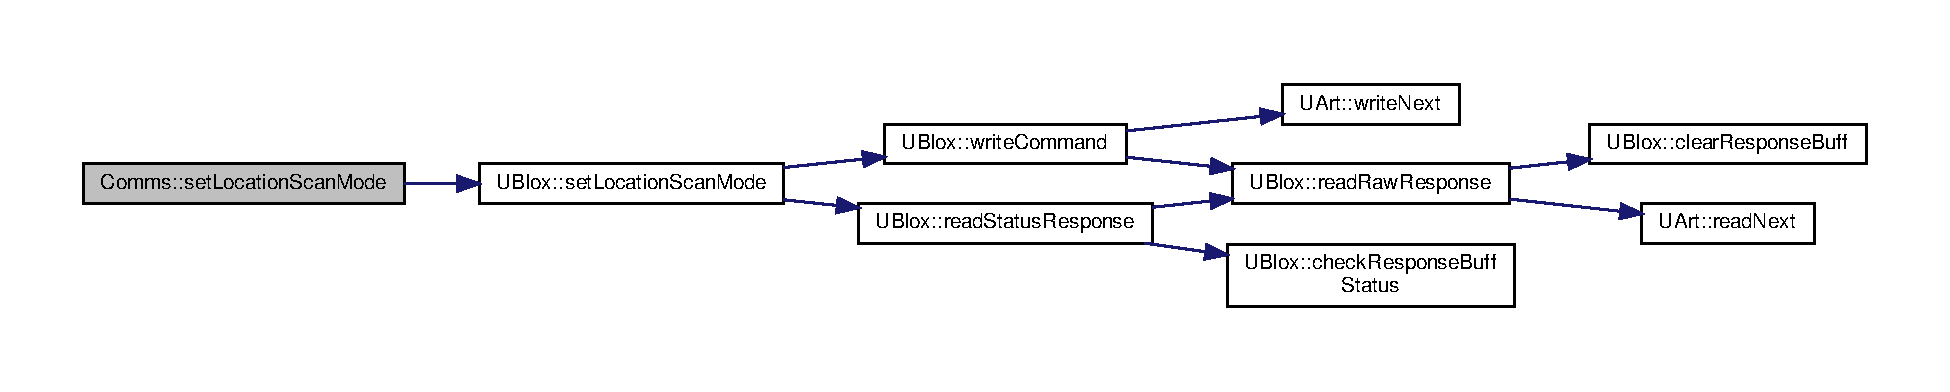
\includegraphics[width=350pt]{d8/dcc/class_comms_a73c0cd58db7daf118bd0b1726fc9dded_cgraph}
\end{center}
\end{figure}
\mbox{\Hypertarget{class_comms_a1b6f5cafba74fc0e175f057e15656362}\label{class_comms_a1b6f5cafba74fc0e175f057e15656362}} 
\index{Comms@{Comms}!set\+Send\+Message\+Mode@{set\+Send\+Message\+Mode}}
\index{set\+Send\+Message\+Mode@{set\+Send\+Message\+Mode}!Comms@{Comms}}
\subsubsection{\texorpdfstring{set\+Send\+Message\+Mode()}{setSendMessageMode()}}
{\footnotesize\ttfamily bool Comms\+::set\+Send\+Message\+Mode (\begin{DoxyParamCaption}\item[{char}]{send\+Msg\+Mode }\end{DoxyParamCaption})}

Setting the send message mode that is to be used for sending text messages to a mobile device.


\begin{DoxyParams}{Parameters}
{\em send\+Msg\+Mode} & The mode that\textquotesingle{}s to be utilised (S\+E\+N\+D\+\_\+\+T\+E\+X\+T\+\_\+\+M\+O\+D\+E\+\_\+\+P\+DU or S\+E\+N\+D\+\_\+\+T\+E\+X\+T\+\_\+\+M\+O\+D\+E\+\_\+\+T\+E\+XT). \\
\hline
\end{DoxyParams}
\begin{DoxyReturn}{Returns}
True if the mode was successfully set, false otherwise. 
\end{DoxyReturn}


Definition at line 230 of file Comms.\+cpp.


\begin{DoxyCode}
231 \{
232     \textcolor{comment}{// Lock the comms interface and set the message mode.}
233     \hyperlink{class_comms_a21df861b1202573e4cd0cb5666d638fe}{mtx}.lock();
234     \textcolor{keywordtype}{bool} rc = \hyperlink{class_comms_ac64dea134b116147e5441172346dbd6c}{uBlox}.\hyperlink{class_u_blox_a12c1042d3bcb503b025927fd53d54243}{setSendMessageMode}(sendMsgMode);
235     \hyperlink{class_comms_a21df861b1202573e4cd0cb5666d638fe}{mtx}.unlock();
236 
237     \textcolor{comment}{// Return the state of the function.}
238     \textcolor{keywordflow}{return} rc;
239 \}
\end{DoxyCode}
Here is the call graph for this function\+:\nopagebreak
\begin{figure}[H]
\begin{center}
\leavevmode
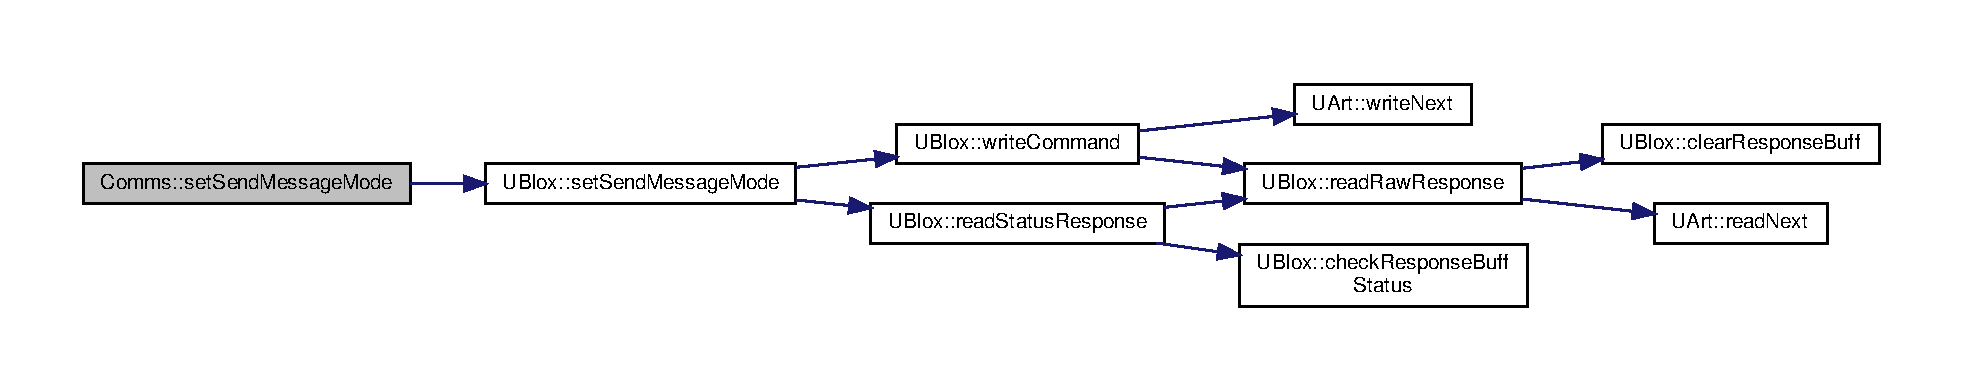
\includegraphics[width=350pt]{d8/dcc/class_comms_a1b6f5cafba74fc0e175f057e15656362_cgraph}
\end{center}
\end{figure}
\mbox{\Hypertarget{class_comms_a9563254514d2f64c0427be2aeaba26d8}\label{class_comms_a9563254514d2f64c0427be2aeaba26d8}} 
\index{Comms@{Comms}!start\+Auto\+Registration@{start\+Auto\+Registration}}
\index{start\+Auto\+Registration@{start\+Auto\+Registration}!Comms@{Comms}}
\subsubsection{\texorpdfstring{start\+Auto\+Registration()}{startAutoRegistration()}}
{\footnotesize\ttfamily bool Comms\+::start\+Auto\+Registration (\begin{DoxyParamCaption}\item[{bool \&}]{registered }\end{DoxyParamCaption})}

Starts the auto registration process if the sim has not already been registered,


\begin{DoxyParams}{Parameters}
{\em registered} & The bool reference into which the auto registration result is to be stored. \\
\hline
\end{DoxyParams}
\begin{DoxyReturn}{Returns}
True if the command was successfully run, false otherwise. 
\end{DoxyReturn}


Definition at line 135 of file Comms.\+cpp.


\begin{DoxyCode}
136 \{
137     \textcolor{comment}{// Lock comms and start the auto registration.}
138     \hyperlink{class_comms_a21df861b1202573e4cd0cb5666d638fe}{mtx}.lock();
139     \textcolor{keywordtype}{bool} rc = \hyperlink{class_comms_ac64dea134b116147e5441172346dbd6c}{uBlox}.\hyperlink{class_u_blox_a2e816e864ebf43743b3f6187e20c2b1f}{startAutoRegistration}(registered);
140     \hyperlink{class_comms_a21df861b1202573e4cd0cb5666d638fe}{mtx}.unlock();
141 
142     \textcolor{comment}{// Return the state of the command.}
143     \textcolor{keywordflow}{return} rc;
144 \}
\end{DoxyCode}
Here is the call graph for this function\+:\nopagebreak
\begin{figure}[H]
\begin{center}
\leavevmode
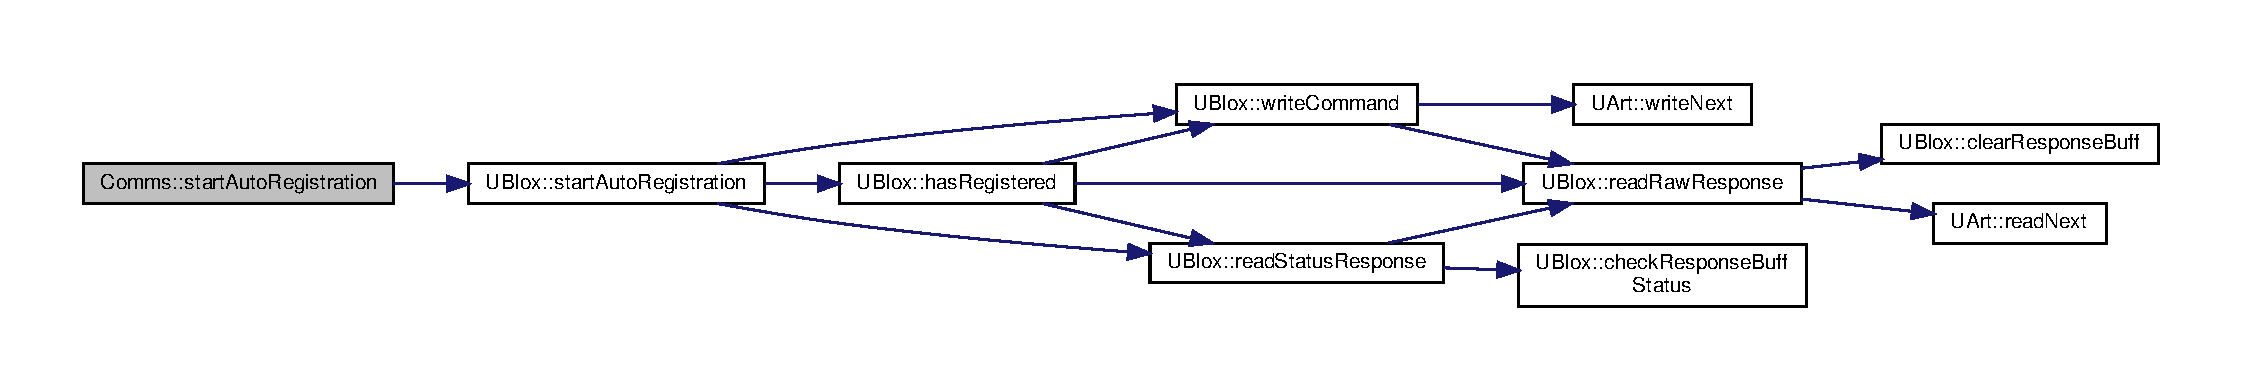
\includegraphics[width=350pt]{d8/dcc/class_comms_a9563254514d2f64c0427be2aeaba26d8_cgraph}
\end{center}
\end{figure}


\subsection{Member Data Documentation}
\mbox{\Hypertarget{class_comms_a21df861b1202573e4cd0cb5666d638fe}\label{class_comms_a21df861b1202573e4cd0cb5666d638fe}} 
\index{Comms@{Comms}!mtx@{mtx}}
\index{mtx@{mtx}!Comms@{Comms}}
\subsubsection{\texorpdfstring{mtx}{mtx}}
{\footnotesize\ttfamily std\+::mutex Comms\+::mtx\hspace{0.3cm}{\ttfamily [private]}}



Definition at line 94 of file Comms.\+h.

\mbox{\Hypertarget{class_comms_ac64dea134b116147e5441172346dbd6c}\label{class_comms_ac64dea134b116147e5441172346dbd6c}} 
\index{Comms@{Comms}!u\+Blox@{u\+Blox}}
\index{u\+Blox@{u\+Blox}!Comms@{Comms}}
\subsubsection{\texorpdfstring{u\+Blox}{uBlox}}
{\footnotesize\ttfamily \hyperlink{class_u_blox}{U\+Blox} Comms\+::u\+Blox\hspace{0.3cm}{\ttfamily [private]}}



Definition at line 91 of file Comms.\+h.



The documentation for this class was generated from the following files\+:\begin{DoxyCompactItemize}
\item 
software/\+Bee\+Safe\+P\+I/src/comms/\hyperlink{_comms_8h}{Comms.\+h}\item 
software/\+Bee\+Safe\+P\+I/src/comms/\hyperlink{_comms_8cpp}{Comms.\+cpp}\end{DoxyCompactItemize}

\hypertarget{class_contact}{}\section{Contact Class Reference}
\label{class_contact}\index{Contact@{Contact}}


The \hyperlink{class_contact}{Contact} class handling the declaration and maintenance of emergency contact information.  




{\ttfamily \#include $<$Contact.\+h$>$}

\subsection*{Public Member Functions}
\begin{DoxyCompactItemize}
\item 
\hyperlink{class_contact_a7851a082367f1d01b04b3f8467b9751c}{Contact} (const std\+::string \&\hyperlink{class_contact_af64e25f3271abad7970293e6adfdf457}{forename}, const std\+::string \&\hyperlink{class_contact_a22518b332de3bd09ed94eb4d9de54894}{surname}, const std\+::string \&\hyperlink{class_contact_abd24eed27b661da4ab20553443212437}{number}, const std\+::string \&\hyperlink{class_contact_a5bc7925e6356e29c9cbad7266f0a4340}{key})
\item 
\hyperlink{class_contact_a9657abb8a68839149c8d928b4c16a82c}{Contact} (const \hyperlink{class_contact}{Contact} \&contact)
\item 
\hyperlink{class_contact_ab68013cc59e3d640735c573e52c35219}{$\sim$\+Contact} ()
\item 
const std\+::string \& \hyperlink{class_contact_a2a2311964fe1a1e48ff41f4ddf355c60}{get\+Forename} ()
\item 
const std\+::string \& \hyperlink{class_contact_aba3d4900ea3173f38b7f296536226bb9}{get\+Surname} ()
\item 
const std\+::string \& \hyperlink{class_contact_a612095b153e05538c32400c4c44cb1aa}{get\+Number} ()
\item 
const std\+::string \& \hyperlink{class_contact_a9be97218caf5efd7dabe2b237d85a22f}{get\+Key} ()
\item 
web\+::json\+::value \hyperlink{class_contact_ae52f56140bbde46dd30cb90dd6cfba4f}{serialise\+Contact} ()
\end{DoxyCompactItemize}
\subsection*{Private Attributes}
\begin{DoxyCompactItemize}
\item 
std\+::string \hyperlink{class_contact_af64e25f3271abad7970293e6adfdf457}{forename}
\item 
std\+::string \hyperlink{class_contact_a22518b332de3bd09ed94eb4d9de54894}{surname}
\item 
std\+::string \hyperlink{class_contact_abd24eed27b661da4ab20553443212437}{number}
\item 
std\+::string \hyperlink{class_contact_a5bc7925e6356e29c9cbad7266f0a4340}{key}
\end{DoxyCompactItemize}


\subsection{Detailed Description}
The \hyperlink{class_contact}{Contact} class handling the declaration and maintenance of emergency contact information. 

The \hyperlink{class_contact}{Contact} class creates the objects containing the information of emergency contacts that must be notified when the device leaves a designated fence area/safe zone, and manages this information\textquotesingle{}s conversion to J\+S\+ON format for the database online.

\begin{DoxyAuthor}{Author}
Bee\+Safe Team, Team 13
\end{DoxyAuthor}
\begin{DoxyVersion}{Version}
v1.\+0
\end{DoxyVersion}
\begin{DoxyDate}{Date}
2020/04/20
\end{DoxyDate}
\hyperlink{class_contact}{Contact}\+: \href{mailto:beesafe.uofg@gmail.com}{\tt beesafe.\+uofg@gmail.\+com}

Licence\+: M\+IT 

Definition at line 38 of file Contact.\+h.



\subsection{Constructor \& Destructor Documentation}
\mbox{\Hypertarget{class_contact_a7851a082367f1d01b04b3f8467b9751c}\label{class_contact_a7851a082367f1d01b04b3f8467b9751c}} 
\index{Contact@{Contact}!Contact@{Contact}}
\index{Contact@{Contact}!Contact@{Contact}}
\subsubsection{\texorpdfstring{Contact()}{Contact()}\hspace{0.1cm}{\footnotesize\ttfamily [1/2]}}
{\footnotesize\ttfamily Contact\+::\+Contact (\begin{DoxyParamCaption}\item[{const std\+::string \&}]{forename,  }\item[{const std\+::string \&}]{surname,  }\item[{const std\+::string \&}]{number,  }\item[{const std\+::string \&}]{key }\end{DoxyParamCaption})}

The explicit constructor for the \hyperlink{class_contact}{Contact} class


\begin{DoxyParams}{Parameters}
{\em forename} & The contact\textquotesingle{}s forename \\
\hline
{\em surname} & The contact\textquotesingle{}s surname \\
\hline
{\em number} & The contact\textquotesingle{}s phone number \\
\hline
{\em key} & The user/contact\textquotesingle{}s A\+PI key \\
\hline
\end{DoxyParams}


Definition at line 34 of file Contact.\+cpp.


\begin{DoxyCode}
36 \{
37     this->\hyperlink{class_contact_af64e25f3271abad7970293e6adfdf457}{forename} = \hyperlink{class_contact_af64e25f3271abad7970293e6adfdf457}{forename};
38     this->\hyperlink{class_contact_a22518b332de3bd09ed94eb4d9de54894}{surname} = \hyperlink{class_contact_a22518b332de3bd09ed94eb4d9de54894}{surname};
39     this->\hyperlink{class_contact_abd24eed27b661da4ab20553443212437}{number} = \hyperlink{class_contact_abd24eed27b661da4ab20553443212437}{number};
40     this->\hyperlink{class_contact_a5bc7925e6356e29c9cbad7266f0a4340}{key} = \hyperlink{class_contact_a5bc7925e6356e29c9cbad7266f0a4340}{key};
41 \}
\end{DoxyCode}
\mbox{\Hypertarget{class_contact_a9657abb8a68839149c8d928b4c16a82c}\label{class_contact_a9657abb8a68839149c8d928b4c16a82c}} 
\index{Contact@{Contact}!Contact@{Contact}}
\index{Contact@{Contact}!Contact@{Contact}}
\subsubsection{\texorpdfstring{Contact()}{Contact()}\hspace{0.1cm}{\footnotesize\ttfamily [2/2]}}
{\footnotesize\ttfamily Contact\+::\+Contact (\begin{DoxyParamCaption}\item[{const \hyperlink{class_contact}{Contact} \&}]{contact }\end{DoxyParamCaption})}

The \hyperlink{class_contact}{Contact} class copy constructor.


\begin{DoxyParams}{Parameters}
{\em contact} & the contact object to be copied \\
\hline
\end{DoxyParams}


Definition at line 48 of file Contact.\+cpp.


\begin{DoxyCode}
49 \{
50     this->\hyperlink{class_contact_af64e25f3271abad7970293e6adfdf457}{forename} = contact.\hyperlink{class_contact_af64e25f3271abad7970293e6adfdf457}{forename};
51     this->\hyperlink{class_contact_a22518b332de3bd09ed94eb4d9de54894}{surname} = contact.\hyperlink{class_contact_a22518b332de3bd09ed94eb4d9de54894}{surname};
52     this->\hyperlink{class_contact_abd24eed27b661da4ab20553443212437}{number} = contact.\hyperlink{class_contact_abd24eed27b661da4ab20553443212437}{number};
53     this->\hyperlink{class_contact_a5bc7925e6356e29c9cbad7266f0a4340}{key} = contact.\hyperlink{class_contact_a5bc7925e6356e29c9cbad7266f0a4340}{key};
54 \}
\end{DoxyCode}
Here is the call graph for this function\+:\nopagebreak
\begin{figure}[H]
\begin{center}
\leavevmode
\includegraphics[width=306pt]{dd/d2a/class_contact_a9657abb8a68839149c8d928b4c16a82c_cgraph}
\end{center}
\end{figure}
\mbox{\Hypertarget{class_contact_ab68013cc59e3d640735c573e52c35219}\label{class_contact_ab68013cc59e3d640735c573e52c35219}} 
\index{Contact@{Contact}!````~Contact@{$\sim$\+Contact}}
\index{````~Contact@{$\sim$\+Contact}!Contact@{Contact}}
\subsubsection{\texorpdfstring{$\sim$\+Contact()}{~Contact()}}
{\footnotesize\ttfamily Contact\+::$\sim$\+Contact (\begin{DoxyParamCaption}{ }\end{DoxyParamCaption})\hspace{0.3cm}{\ttfamily [default]}}

The \hyperlink{class_contact}{Contact} class destructor. Here is the caller graph for this function\+:\nopagebreak
\begin{figure}[H]
\begin{center}
\leavevmode
\includegraphics[width=306pt]{dd/d2a/class_contact_ab68013cc59e3d640735c573e52c35219_icgraph}
\end{center}
\end{figure}


\subsection{Member Function Documentation}
\mbox{\Hypertarget{class_contact_a2a2311964fe1a1e48ff41f4ddf355c60}\label{class_contact_a2a2311964fe1a1e48ff41f4ddf355c60}} 
\index{Contact@{Contact}!get\+Forename@{get\+Forename}}
\index{get\+Forename@{get\+Forename}!Contact@{Contact}}
\subsubsection{\texorpdfstring{get\+Forename()}{getForename()}}
{\footnotesize\ttfamily const std\+::string \& Contact\+::get\+Forename (\begin{DoxyParamCaption}{ }\end{DoxyParamCaption})}

A getter for the first name of the contact. A public accessor for an otherwise private variable.

\begin{DoxyReturn}{Returns}
the contact\textquotesingle{}s forename 
\end{DoxyReturn}


Definition at line 67 of file Contact.\+cpp.


\begin{DoxyCode}
68 \{
69     \textcolor{keywordflow}{return} \hyperlink{class_contact_af64e25f3271abad7970293e6adfdf457}{forename};
70 \}
\end{DoxyCode}
\mbox{\Hypertarget{class_contact_a9be97218caf5efd7dabe2b237d85a22f}\label{class_contact_a9be97218caf5efd7dabe2b237d85a22f}} 
\index{Contact@{Contact}!get\+Key@{get\+Key}}
\index{get\+Key@{get\+Key}!Contact@{Contact}}
\subsubsection{\texorpdfstring{get\+Key()}{getKey()}}
{\footnotesize\ttfamily const std\+::string \& Contact\+::get\+Key (\begin{DoxyParamCaption}{ }\end{DoxyParamCaption})}

A getter for the A\+PI key of the contact. A public accessor for an otherwise private variable.

\begin{DoxyReturn}{Returns}
the contact/user A\+PI key 
\end{DoxyReturn}


Definition at line 100 of file Contact.\+cpp.


\begin{DoxyCode}
101 \{
102     \textcolor{keywordflow}{return} \hyperlink{class_contact_a5bc7925e6356e29c9cbad7266f0a4340}{key};
103 \}
\end{DoxyCode}
\mbox{\Hypertarget{class_contact_a612095b153e05538c32400c4c44cb1aa}\label{class_contact_a612095b153e05538c32400c4c44cb1aa}} 
\index{Contact@{Contact}!get\+Number@{get\+Number}}
\index{get\+Number@{get\+Number}!Contact@{Contact}}
\subsubsection{\texorpdfstring{get\+Number()}{getNumber()}}
{\footnotesize\ttfamily const std\+::string \& Contact\+::get\+Number (\begin{DoxyParamCaption}{ }\end{DoxyParamCaption})}

A getter for the number of the contact. A public accessor for an otherwise private variable.

\begin{DoxyReturn}{Returns}
the contact phone number 
\end{DoxyReturn}


Definition at line 89 of file Contact.\+cpp.


\begin{DoxyCode}
90 \{
91     \textcolor{keywordflow}{return} \hyperlink{class_contact_abd24eed27b661da4ab20553443212437}{number};
92 \}
\end{DoxyCode}
Here is the caller graph for this function\+:\nopagebreak
\begin{figure}[H]
\begin{center}
\leavevmode
\includegraphics[width=350pt]{dd/d2a/class_contact_a612095b153e05538c32400c4c44cb1aa_icgraph}
\end{center}
\end{figure}
\mbox{\Hypertarget{class_contact_aba3d4900ea3173f38b7f296536226bb9}\label{class_contact_aba3d4900ea3173f38b7f296536226bb9}} 
\index{Contact@{Contact}!get\+Surname@{get\+Surname}}
\index{get\+Surname@{get\+Surname}!Contact@{Contact}}
\subsubsection{\texorpdfstring{get\+Surname()}{getSurname()}}
{\footnotesize\ttfamily const std\+::string \& Contact\+::get\+Surname (\begin{DoxyParamCaption}{ }\end{DoxyParamCaption})}

A getter for the last name of the contact. A public accessor for an otherwise private variable.

\begin{DoxyReturn}{Returns}
the contact\textquotesingle{}s surname. 
\end{DoxyReturn}


Definition at line 78 of file Contact.\+cpp.


\begin{DoxyCode}
79 \{
80     \textcolor{keywordflow}{return} \hyperlink{class_contact_a22518b332de3bd09ed94eb4d9de54894}{surname};
81 \}
\end{DoxyCode}
\mbox{\Hypertarget{class_contact_ae52f56140bbde46dd30cb90dd6cfba4f}\label{class_contact_ae52f56140bbde46dd30cb90dd6cfba4f}} 
\index{Contact@{Contact}!serialise\+Contact@{serialise\+Contact}}
\index{serialise\+Contact@{serialise\+Contact}!Contact@{Contact}}
\subsubsection{\texorpdfstring{serialise\+Contact()}{serialiseContact()}}
{\footnotesize\ttfamily web\+::json\+::value Contact\+::serialise\+Contact (\begin{DoxyParamCaption}{ }\end{DoxyParamCaption})}

A method to serialise the contact into a J\+S\+ON element.

\begin{DoxyReturn}{Returns}
a J\+S\+ON object containing the \hyperlink{class_contact}{Contact} information 
\end{DoxyReturn}


Definition at line 110 of file Contact.\+cpp.


\begin{DoxyCode}
111 \{
112     web::json::value jsonContact = web::json::value::object();
113     jsonContact[utility::string\_t(U(\hyperlink{_contact_8h_a18b1ad44af79fea17bfed22ff66f94f8}{JSON\_KEY\_CONTACT\_FORENAME}))] = 
      web::json::value::string(U(\hyperlink{class_contact_af64e25f3271abad7970293e6adfdf457}{forename}));
114     jsonContact[utility::string\_t(U(\hyperlink{_contact_8h_a579318fe639c3cf3628817c4090be13e}{JSON\_KEY\_CONTACT\_SURNAME}))] = 
      web::json::value::string(U(\hyperlink{class_contact_a22518b332de3bd09ed94eb4d9de54894}{surname}));
115     jsonContact[utility::string\_t(U(\hyperlink{_contact_8h_a97dc3d327e5283642c81bc7d6a572ced}{JSON\_KEY\_CONTACT\_NUMBER}))] = 
      web::json::value::string(U(\hyperlink{class_contact_abd24eed27b661da4ab20553443212437}{number}));
116     jsonContact[utility::string\_t(U(\hyperlink{_contact_8h_a90f2095b835454d47c72995503684937}{JSON\_KEY\_CONTACT\_KEY}))] = web::json::value::string(
      U(\hyperlink{class_contact_a5bc7925e6356e29c9cbad7266f0a4340}{key}));
117     \textcolor{keywordflow}{return} jsonContact;
118 \}
\end{DoxyCode}


\subsection{Member Data Documentation}
\mbox{\Hypertarget{class_contact_af64e25f3271abad7970293e6adfdf457}\label{class_contact_af64e25f3271abad7970293e6adfdf457}} 
\index{Contact@{Contact}!forename@{forename}}
\index{forename@{forename}!Contact@{Contact}}
\subsubsection{\texorpdfstring{forename}{forename}}
{\footnotesize\ttfamily std\+::string Contact\+::forename\hspace{0.3cm}{\ttfamily [private]}}



Definition at line 63 of file Contact.\+h.

\mbox{\Hypertarget{class_contact_a5bc7925e6356e29c9cbad7266f0a4340}\label{class_contact_a5bc7925e6356e29c9cbad7266f0a4340}} 
\index{Contact@{Contact}!key@{key}}
\index{key@{key}!Contact@{Contact}}
\subsubsection{\texorpdfstring{key}{key}}
{\footnotesize\ttfamily std\+::string Contact\+::key\hspace{0.3cm}{\ttfamily [private]}}



Definition at line 66 of file Contact.\+h.

\mbox{\Hypertarget{class_contact_abd24eed27b661da4ab20553443212437}\label{class_contact_abd24eed27b661da4ab20553443212437}} 
\index{Contact@{Contact}!number@{number}}
\index{number@{number}!Contact@{Contact}}
\subsubsection{\texorpdfstring{number}{number}}
{\footnotesize\ttfamily std\+::string Contact\+::number\hspace{0.3cm}{\ttfamily [private]}}



Definition at line 65 of file Contact.\+h.

\mbox{\Hypertarget{class_contact_a22518b332de3bd09ed94eb4d9de54894}\label{class_contact_a22518b332de3bd09ed94eb4d9de54894}} 
\index{Contact@{Contact}!surname@{surname}}
\index{surname@{surname}!Contact@{Contact}}
\subsubsection{\texorpdfstring{surname}{surname}}
{\footnotesize\ttfamily std\+::string Contact\+::surname\hspace{0.3cm}{\ttfamily [private]}}



Definition at line 64 of file Contact.\+h.



The documentation for this class was generated from the following files\+:\begin{DoxyCompactItemize}
\item 
software/\+Bee\+Safe\+P\+I/src/contact/\hyperlink{_contact_8h}{Contact.\+h}\item 
software/\+Bee\+Safe\+P\+I/src/contact/\hyperlink{_contact_8cpp}{Contact.\+cpp}\end{DoxyCompactItemize}

\hypertarget{class_fence}{}\section{Fence Class Reference}
\label{class_fence}\index{Fence@{Fence}}


The \hyperlink{class_fence}{Fence} parent class providing generic functionality for handling fences.  




{\ttfamily \#include $<$Fence.\+h$>$}



Inheritance diagram for Fence\+:\nopagebreak
\begin{figure}[H]
\begin{center}
\leavevmode
\includegraphics[width=234pt]{dc/d62/class_fence__inherit__graph}
\end{center}
\end{figure}
\subsection*{Public Member Functions}
\begin{DoxyCompactItemize}
\item 
\hyperlink{class_fence_a5c2be718e885ed9ae2ca048406d126b3}{Fence} (std\+::string \&\hyperlink{class_fence_aa405676733f25812b38ea0dd9ccd1863}{name}, bool \hyperlink{class_fence_ad570430040eee657c625a67d5589c4b5}{safe}, const std\+::map$<$ int, std\+::vector$<$ std\+::pair$<$ std\+::tm, std\+::tm $>$$>$$>$ \&\hyperlink{class_fence_ae589e973fa03316847aeceedd72e2b64}{week})
\item 
\hyperlink{class_fence_ae67f4594ce0f96eda5cb02df41fcf45a}{Fence} (std\+::string \&\hyperlink{class_fence_aa405676733f25812b38ea0dd9ccd1863}{name}, bool \hyperlink{class_fence_ad570430040eee657c625a67d5589c4b5}{safe})
\item 
\hyperlink{class_fence_a3fdfc7240f1e938dab4c9534c63aa427}{Fence} (const \hyperlink{class_fence}{Fence} \&fence)
\item 
virtual \hyperlink{class_fence_a6c5e019535f94462bfab1ad19b865c55}{$\sim$\+Fence} ()=0
\item 
std\+::string \& \hyperlink{class_fence_a1d90d0ff61bec6cda8240f6365fc5d28}{get\+Name} ()
\item 
const std\+::map$<$ int, std\+::vector$<$ std\+::pair$<$ std\+::tm, std\+::tm $>$ $>$ $>$ \& \hyperlink{class_fence_a533d7eaba8b2d6774ec2c9dce05145eb}{get\+Week} ()
\item 
const std\+::vector$<$ std\+::pair$<$ std\+::tm, std\+::tm $>$ $>$ \& \hyperlink{class_fence_a818ee0fcbac0c2f9262a48916a79d73c}{get\+Times} (int day)
\item 
bool \hyperlink{class_fence_a4f0626e3b3189b6ab1c505c92952bcb2}{is\+Safe} ()
\item 
bool \hyperlink{class_fence_a7695b0f94f461369703188a287a38ab4}{is\+In\+Time} ()
\item 
bool \hyperlink{class_fence_a9d1d90f134dceb2168247cd8454d91f4}{is\+In\+Time} (const std\+::time\+\_\+t \&time)
\item 
virtual bool \hyperlink{class_fence_a80fb7fbb60592d3e8afc0ecb5122b987}{is\+In\+Location} (std\+::pair$<$ double, double $>$ \&lat\+Lng)=0
\item 
virtual web\+::json\+::value \hyperlink{class_fence_a5c8529e80a4444cc9ca0fb660cbf07c8}{serialise\+Fence} ()
\item 
bool \hyperlink{class_fence_a224ef2ce3f97de067f996b4722c66797}{is\+Inside} (std\+::pair$<$ double, double $>$ \&lat\+Lng)
\end{DoxyCompactItemize}
\subsection*{Private Attributes}
\begin{DoxyCompactItemize}
\item 
std\+::string \hyperlink{class_fence_aa405676733f25812b38ea0dd9ccd1863}{name}
\item 
bool \hyperlink{class_fence_ad570430040eee657c625a67d5589c4b5}{safe}
\item 
std\+::map$<$ int, std\+::vector$<$ std\+::pair$<$ std\+::tm, std\+::tm $>$ $>$ $>$ \hyperlink{class_fence_ae589e973fa03316847aeceedd72e2b64}{week}
\end{DoxyCompactItemize}


\subsection{Detailed Description}
The \hyperlink{class_fence}{Fence} parent class providing generic functionality for handling fences. 

The \hyperlink{class_fence}{Fence} class is the parent class to the Poly-\/ and \hyperlink{class_round_fence}{Round\+Fence} classes. It provides methods to create and manage the details of fences regardless of type, such as what times on what days is it considered a safezone, checks if the device is within the time and physical boundaries of the location they are at, and provides a super function to converting the \hyperlink{class_fence}{Fence} objects into J\+S\+ON objects to be handled by the online database.

\begin{DoxyAuthor}{Author}
Bee\+Safe Team, Team 13
\end{DoxyAuthor}
\begin{DoxyVersion}{Version}
v1.\+0
\end{DoxyVersion}
\begin{DoxyDate}{Date}
2020/04/20
\end{DoxyDate}
\hyperlink{class_contact}{Contact}\+: \href{mailto:beesafe.uofg@gmail.com}{\tt beesafe.\+uofg@gmail.\+com}

Licence\+: M\+IT 

Definition at line 50 of file Fence.\+h.



\subsection{Constructor \& Destructor Documentation}
\mbox{\Hypertarget{class_fence_a5c2be718e885ed9ae2ca048406d126b3}\label{class_fence_a5c2be718e885ed9ae2ca048406d126b3}} 
\index{Fence@{Fence}!Fence@{Fence}}
\index{Fence@{Fence}!Fence@{Fence}}
\subsubsection{\texorpdfstring{Fence()}{Fence()}\hspace{0.1cm}{\footnotesize\ttfamily [1/3]}}
{\footnotesize\ttfamily Fence\+::\+Fence (\begin{DoxyParamCaption}\item[{std\+::string \&}]{name,  }\item[{bool}]{safe,  }\item[{const std\+::map$<$ int, std\+::vector$<$ std\+::pair$<$ std\+::tm, std\+::tm $>$$>$$>$ \&}]{week }\end{DoxyParamCaption})}



Definition at line 36 of file Fence.\+cpp.


\begin{DoxyCode}
38 \{
39     this->\hyperlink{class_fence_aa405676733f25812b38ea0dd9ccd1863}{name} = \hyperlink{class_fence_aa405676733f25812b38ea0dd9ccd1863}{name};
40     this->\hyperlink{class_fence_ad570430040eee657c625a67d5589c4b5}{safe} = \hyperlink{class_fence_ad570430040eee657c625a67d5589c4b5}{safe};
41     this->\hyperlink{class_fence_ae589e973fa03316847aeceedd72e2b64}{week} = \hyperlink{class_fence_ae589e973fa03316847aeceedd72e2b64}{week};
42 \}
\end{DoxyCode}
\mbox{\Hypertarget{class_fence_ae67f4594ce0f96eda5cb02df41fcf45a}\label{class_fence_ae67f4594ce0f96eda5cb02df41fcf45a}} 
\index{Fence@{Fence}!Fence@{Fence}}
\index{Fence@{Fence}!Fence@{Fence}}
\subsubsection{\texorpdfstring{Fence()}{Fence()}\hspace{0.1cm}{\footnotesize\ttfamily [2/3]}}
{\footnotesize\ttfamily Fence\+::\+Fence (\begin{DoxyParamCaption}\item[{std\+::string \&}]{name,  }\item[{bool}]{safe }\end{DoxyParamCaption})}



Definition at line 45 of file Fence.\+cpp.


\begin{DoxyCode}
46 \{
47     this->\hyperlink{class_fence_aa405676733f25812b38ea0dd9ccd1863}{name} = \hyperlink{class_fence_aa405676733f25812b38ea0dd9ccd1863}{name};
48     this->\hyperlink{class_fence_ad570430040eee657c625a67d5589c4b5}{safe} = \hyperlink{class_fence_ad570430040eee657c625a67d5589c4b5}{safe};
49 \}
\end{DoxyCode}
\mbox{\Hypertarget{class_fence_a3fdfc7240f1e938dab4c9534c63aa427}\label{class_fence_a3fdfc7240f1e938dab4c9534c63aa427}} 
\index{Fence@{Fence}!Fence@{Fence}}
\index{Fence@{Fence}!Fence@{Fence}}
\subsubsection{\texorpdfstring{Fence()}{Fence()}\hspace{0.1cm}{\footnotesize\ttfamily [3/3]}}
{\footnotesize\ttfamily Fence\+::\+Fence (\begin{DoxyParamCaption}\item[{const \hyperlink{class_fence}{Fence} \&}]{fence }\end{DoxyParamCaption})}



Definition at line 52 of file Fence.\+cpp.


\begin{DoxyCode}
52                                \{
53     this->\hyperlink{class_fence_aa405676733f25812b38ea0dd9ccd1863}{name} = fence.\hyperlink{class_fence_aa405676733f25812b38ea0dd9ccd1863}{name};
54     this->\hyperlink{class_fence_ad570430040eee657c625a67d5589c4b5}{safe} = fence.\hyperlink{class_fence_ad570430040eee657c625a67d5589c4b5}{safe};
55     this->\hyperlink{class_fence_ae589e973fa03316847aeceedd72e2b64}{week} = fence.\hyperlink{class_fence_ae589e973fa03316847aeceedd72e2b64}{week};
56 \}
\end{DoxyCode}
Here is the call graph for this function\+:\nopagebreak
\begin{figure}[H]
\begin{center}
\leavevmode
\includegraphics[width=276pt]{d0/db8/class_fence_a3fdfc7240f1e938dab4c9534c63aa427_cgraph}
\end{center}
\end{figure}
\mbox{\Hypertarget{class_fence_a6c5e019535f94462bfab1ad19b865c55}\label{class_fence_a6c5e019535f94462bfab1ad19b865c55}} 
\index{Fence@{Fence}!````~Fence@{$\sim$\+Fence}}
\index{````~Fence@{$\sim$\+Fence}!Fence@{Fence}}
\subsubsection{\texorpdfstring{$\sim$\+Fence()}{~Fence()}}
{\footnotesize\ttfamily Fence\+::$\sim$\+Fence (\begin{DoxyParamCaption}{ }\end{DoxyParamCaption})\hspace{0.3cm}{\ttfamily [pure virtual]}, {\ttfamily [default]}}

Here is the caller graph for this function\+:\nopagebreak
\begin{figure}[H]
\begin{center}
\leavevmode
\includegraphics[width=276pt]{d0/db8/class_fence_a6c5e019535f94462bfab1ad19b865c55_icgraph}
\end{center}
\end{figure}


\subsection{Member Function Documentation}
\mbox{\Hypertarget{class_fence_a1d90d0ff61bec6cda8240f6365fc5d28}\label{class_fence_a1d90d0ff61bec6cda8240f6365fc5d28}} 
\index{Fence@{Fence}!get\+Name@{get\+Name}}
\index{get\+Name@{get\+Name}!Fence@{Fence}}
\subsubsection{\texorpdfstring{get\+Name()}{getName()}}
{\footnotesize\ttfamily std\+::string \& Fence\+::get\+Name (\begin{DoxyParamCaption}{ }\end{DoxyParamCaption})}



Definition at line 61 of file Fence.\+cpp.


\begin{DoxyCode}
62 \{
63     \textcolor{keywordflow}{return} \hyperlink{class_fence_aa405676733f25812b38ea0dd9ccd1863}{name};
64 \}
\end{DoxyCode}
Here is the call graph for this function\+:\nopagebreak
\begin{figure}[H]
\begin{center}
\leavevmode
\includegraphics[width=307pt]{d0/db8/class_fence_a1d90d0ff61bec6cda8240f6365fc5d28_cgraph}
\end{center}
\end{figure}
Here is the caller graph for this function\+:\nopagebreak
\begin{figure}[H]
\begin{center}
\leavevmode
\includegraphics[width=305pt]{d0/db8/class_fence_a1d90d0ff61bec6cda8240f6365fc5d28_icgraph}
\end{center}
\end{figure}
\mbox{\Hypertarget{class_fence_a818ee0fcbac0c2f9262a48916a79d73c}\label{class_fence_a818ee0fcbac0c2f9262a48916a79d73c}} 
\index{Fence@{Fence}!get\+Times@{get\+Times}}
\index{get\+Times@{get\+Times}!Fence@{Fence}}
\subsubsection{\texorpdfstring{get\+Times()}{getTimes()}}
{\footnotesize\ttfamily const std\+::vector$<$ std\+::pair$<$ std\+::tm, std\+::tm $>$ $>$ \& Fence\+::get\+Times (\begin{DoxyParamCaption}\item[{int}]{day }\end{DoxyParamCaption})}



Definition at line 76 of file Fence.\+cpp.


\begin{DoxyCode}
76                                                                      \{
77     \textcolor{keywordflow}{return} \hyperlink{class_fence_ae589e973fa03316847aeceedd72e2b64}{week}[day];
78 \}
\end{DoxyCode}
\mbox{\Hypertarget{class_fence_a533d7eaba8b2d6774ec2c9dce05145eb}\label{class_fence_a533d7eaba8b2d6774ec2c9dce05145eb}} 
\index{Fence@{Fence}!get\+Week@{get\+Week}}
\index{get\+Week@{get\+Week}!Fence@{Fence}}
\subsubsection{\texorpdfstring{get\+Week()}{getWeek()}}
{\footnotesize\ttfamily const std\+::map$<$ int, std\+::vector$<$ std\+::pair$<$ std\+::tm, std\+::tm $>$ $>$ $>$ \& Fence\+::get\+Week (\begin{DoxyParamCaption}{ }\end{DoxyParamCaption})}



Definition at line 71 of file Fence.\+cpp.


\begin{DoxyCode}
71                                                                     \{
72     \textcolor{keywordflow}{return} \hyperlink{class_fence_ae589e973fa03316847aeceedd72e2b64}{week};
73 \}
\end{DoxyCode}
\mbox{\Hypertarget{class_fence_a80fb7fbb60592d3e8afc0ecb5122b987}\label{class_fence_a80fb7fbb60592d3e8afc0ecb5122b987}} 
\index{Fence@{Fence}!is\+In\+Location@{is\+In\+Location}}
\index{is\+In\+Location@{is\+In\+Location}!Fence@{Fence}}
\subsubsection{\texorpdfstring{is\+In\+Location()}{isInLocation()}}
{\footnotesize\ttfamily virtual bool Fence\+::is\+In\+Location (\begin{DoxyParamCaption}\item[{std\+::pair$<$ double, double $>$ \&}]{lat\+Lng }\end{DoxyParamCaption})\hspace{0.3cm}{\ttfamily [pure virtual]}}



Implemented in \hyperlink{class_poly_fence_af8116af5be86f8426102985c3dbcdf5e}{Poly\+Fence}, and \hyperlink{class_round_fence_a4955bf0dbd168853ba9913465953865d}{Round\+Fence}.

Here is the caller graph for this function\+:\nopagebreak
\begin{figure}[H]
\begin{center}
\leavevmode
\includegraphics[width=350pt]{d0/db8/class_fence_a80fb7fbb60592d3e8afc0ecb5122b987_icgraph}
\end{center}
\end{figure}
\mbox{\Hypertarget{class_fence_a224ef2ce3f97de067f996b4722c66797}\label{class_fence_a224ef2ce3f97de067f996b4722c66797}} 
\index{Fence@{Fence}!is\+Inside@{is\+Inside}}
\index{is\+Inside@{is\+Inside}!Fence@{Fence}}
\subsubsection{\texorpdfstring{is\+Inside()}{isInside()}}
{\footnotesize\ttfamily bool Fence\+::is\+Inside (\begin{DoxyParamCaption}\item[{std\+::pair$<$ double, double $>$ \&}]{lat\+Lng }\end{DoxyParamCaption})}



Definition at line 134 of file Fence.\+cpp.


\begin{DoxyCode}
134                                                     \{
135     \textcolor{keywordflow}{return}( this->\hyperlink{class_fence_a7695b0f94f461369703188a287a38ab4}{isInTime}() && this->\hyperlink{class_fence_a80fb7fbb60592d3e8afc0ecb5122b987}{isInLocation}(latLng));
136 \}
\end{DoxyCode}
Here is the call graph for this function\+:\nopagebreak
\begin{figure}[H]
\begin{center}
\leavevmode
\includegraphics[width=301pt]{d0/db8/class_fence_a224ef2ce3f97de067f996b4722c66797_cgraph}
\end{center}
\end{figure}
\mbox{\Hypertarget{class_fence_a7695b0f94f461369703188a287a38ab4}\label{class_fence_a7695b0f94f461369703188a287a38ab4}} 
\index{Fence@{Fence}!is\+In\+Time@{is\+In\+Time}}
\index{is\+In\+Time@{is\+In\+Time}!Fence@{Fence}}
\subsubsection{\texorpdfstring{is\+In\+Time()}{isInTime()}\hspace{0.1cm}{\footnotesize\ttfamily [1/2]}}
{\footnotesize\ttfamily bool Fence\+::is\+In\+Time (\begin{DoxyParamCaption}{ }\end{DoxyParamCaption})}



Definition at line 86 of file Fence.\+cpp.


\begin{DoxyCode}
86                      \{
87     \textcolor{keyword}{const} std::time\_t systemTime = std::time(\textcolor{keyword}{nullptr});
88     \textcolor{keywordflow}{return} \hyperlink{class_fence_a7695b0f94f461369703188a287a38ab4}{isInTime}(systemTime);
89 \}
\end{DoxyCode}
Here is the caller graph for this function\+:\nopagebreak
\begin{figure}[H]
\begin{center}
\leavevmode
\includegraphics[width=350pt]{d0/db8/class_fence_a7695b0f94f461369703188a287a38ab4_icgraph}
\end{center}
\end{figure}
\mbox{\Hypertarget{class_fence_a9d1d90f134dceb2168247cd8454d91f4}\label{class_fence_a9d1d90f134dceb2168247cd8454d91f4}} 
\index{Fence@{Fence}!is\+In\+Time@{is\+In\+Time}}
\index{is\+In\+Time@{is\+In\+Time}!Fence@{Fence}}
\subsubsection{\texorpdfstring{is\+In\+Time()}{isInTime()}\hspace{0.1cm}{\footnotesize\ttfamily [2/2]}}
{\footnotesize\ttfamily bool Fence\+::is\+In\+Time (\begin{DoxyParamCaption}\item[{const std\+::time\+\_\+t \&}]{time }\end{DoxyParamCaption})}



Definition at line 93 of file Fence.\+cpp.


\begin{DoxyCode}
93                                           \{
94 
95     \textcolor{comment}{// Extract information from system time.}
96     std::tm time\_tm = *std::localtime(&time);
97     \textcolor{keyword}{auto} iter = \hyperlink{class_fence_ae589e973fa03316847aeceedd72e2b64}{week}.find(time\_tm.tm\_wday);
98 
99     \textcolor{comment}{// Check if time information exists.}
100     \textcolor{keywordflow}{if} (iter == \hyperlink{class_fence_ae589e973fa03316847aeceedd72e2b64}{week}.end()) \{
101         \textcolor{keywordflow}{return} \textcolor{keyword}{true};
102     \} \textcolor{keywordflow}{else} \textcolor{keywordflow}{if} (iter->second.empty()) \{
103         \textcolor{keywordflow}{return} \textcolor{keyword}{true};
104     \}
105 
106     \textcolor{comment}{// Iterate through days list of from and to times.}
107     \textcolor{keyword}{auto} &dayTimes = iter->second;
108     \textcolor{keywordflow}{for} (\textcolor{keyword}{const} std::pair<std::tm, std::tm> &dayTime : dayTimes) \{
109 
110         \textcolor{comment}{// If time is before from time, we are not present.}
111         \textcolor{keywordflow}{if} (time\_tm.tm\_hour < dayTime.first.tm\_hour) \{
112             \textcolor{keywordflow}{return} \textcolor{keyword}{false};
113         \} \textcolor{keywordflow}{else} \textcolor{keywordflow}{if} (time\_tm.tm\_hour == dayTime.first.tm\_hour) \{
114             \textcolor{keywordflow}{if} (time\_tm.tm\_min < dayTime.first.tm\_min) \{
115                 \textcolor{keywordflow}{return} \textcolor{keyword}{false};
116             \}
117         \}
118 
119         \textcolor{comment}{// If the time is after the to time, we are not present.}
120         \textcolor{keywordflow}{if} (time\_tm.tm\_hour > dayTime.second.tm\_hour) \{
121             \textcolor{keywordflow}{return} \textcolor{keyword}{false};
122         \} \textcolor{keywordflow}{else} \textcolor{keywordflow}{if} (time\_tm.tm\_hour == dayTime.second.tm\_hour) \{
123             \textcolor{keywordflow}{if} (time\_tm.tm\_min > dayTime.second.tm\_min) \{
124                 \textcolor{keywordflow}{return} \textcolor{keyword}{false};
125             \}
126         \}
127     \}
128 
129     \textcolor{comment}{// By default the user is within the fence.}
130     \textcolor{keywordflow}{return} \textcolor{keyword}{true};
131 \}
\end{DoxyCode}
\mbox{\Hypertarget{class_fence_a4f0626e3b3189b6ab1c505c92952bcb2}\label{class_fence_a4f0626e3b3189b6ab1c505c92952bcb2}} 
\index{Fence@{Fence}!is\+Safe@{is\+Safe}}
\index{is\+Safe@{is\+Safe}!Fence@{Fence}}
\subsubsection{\texorpdfstring{is\+Safe()}{isSafe()}}
{\footnotesize\ttfamily bool Fence\+::is\+Safe (\begin{DoxyParamCaption}{ }\end{DoxyParamCaption})}



Definition at line 81 of file Fence.\+cpp.


\begin{DoxyCode}
81                    \{
82     \textcolor{keywordflow}{return} \hyperlink{class_fence_ad570430040eee657c625a67d5589c4b5}{safe};
83 \}
\end{DoxyCode}
\mbox{\Hypertarget{class_fence_a5c8529e80a4444cc9ca0fb660cbf07c8}\label{class_fence_a5c8529e80a4444cc9ca0fb660cbf07c8}} 
\index{Fence@{Fence}!serialise\+Fence@{serialise\+Fence}}
\index{serialise\+Fence@{serialise\+Fence}!Fence@{Fence}}
\subsubsection{\texorpdfstring{serialise\+Fence()}{serialiseFence()}}
{\footnotesize\ttfamily web\+::json\+::value Fence\+::serialise\+Fence (\begin{DoxyParamCaption}{ }\end{DoxyParamCaption})\hspace{0.3cm}{\ttfamily [virtual]}}



Reimplemented in \hyperlink{class_poly_fence_ae748da10e4fd15f87b74e0d996f00103}{Poly\+Fence}, and \hyperlink{class_round_fence_ae9dd3e4291f7509ce557a6c28cdd682d}{Round\+Fence}.



Definition at line 139 of file Fence.\+cpp.


\begin{DoxyCode}
139                                    \{
140 
141 
142     \textcolor{comment}{// The list of day names and the fence root element, respectively.}
143     \textcolor{keyword}{const} std::string days[] = \hyperlink{_fence_8h_a189c5645c45c0d8943719ee620afa4b2}{JSON\_KEY\_FENCE\_DAYS};
144     \textcolor{keywordtype}{char} dayTimeBuffer[\hyperlink{_fence_8cpp_a69b35d746bf626a8192e75810e701320}{DAY\_TIME\_BUFFER\_SIZE}];
145 
146     \textcolor{comment}{// The root fence json element.}
147     web::json::value jsonFence = web::json::value::object();
148 
149     \textcolor{comment}{// Serialise the name and safety of the fence.}
150     jsonFence[U(\hyperlink{_fence_8h_a0bf10e901f60610c8a47c143051deea4}{JSON\_KEY\_FENCE\_NAME})] = web::json::value::string(
      \hyperlink{class_fence_aa405676733f25812b38ea0dd9ccd1863}{name});
151     jsonFence[U(\hyperlink{_fence_8h_a4b2bc1fec134d7881cd286c8b6741752}{JSON\_KEY\_FENCE\_SAFE})] = web::json::value::boolean(
      \hyperlink{class_fence_ad570430040eee657c625a67d5589c4b5}{safe});
152 
153     \textcolor{comment}{// Serialise the week i.e. days and times.}
154     jsonFence[U(\hyperlink{_fence_8h_a94c5efe13ae824c55eebaa9e8a76dd57}{JSON\_KEY\_FENCE\_WEEK})] = web::json::value::object();
155     \textcolor{keywordflow}{for} (\textcolor{keyword}{auto} &day : \hyperlink{class_fence_ae589e973fa03316847aeceedd72e2b64}{week}) \{
156         \textcolor{keywordflow}{for} (\textcolor{keywordtype}{int} i = 0; i < day.second.size(); ++i) \{
157 
158             \textcolor{comment}{// Format the string that's to be written.}
159             snprintf(dayTimeBuffer,
160                      \hyperlink{_fence_8cpp_a69b35d746bf626a8192e75810e701320}{DAY\_TIME\_BUFFER\_SIZE},
161                      \hyperlink{_fence_8cpp_aa7662fb39f778fae608e70d079dc11ea}{DAY\_TIME\_STRING\_FORMAT},
162                      day.second[i].first.tm\_hour,
163                      day.second[i].first.tm\_min
164             );
165 
166             \textcolor{comment}{// serialise the from time.}
167             jsonFence[U(\hyperlink{_fence_8h_a94c5efe13ae824c55eebaa9e8a76dd57}{JSON\_KEY\_FENCE\_WEEK})][days[day.first]][i][U(
      \hyperlink{_fence_8h_a7993b3aacbec44628f2d9ab7df6ff5b9}{JSON\_KEY\_FENCE\_TIME\_FROM})]
168                     = web::json::value::string(U(dayTimeBuffer));
169 
170             \textcolor{comment}{// Format the string that's to be written.}
171             snprintf(dayTimeBuffer,
172                      \hyperlink{_fence_8cpp_a69b35d746bf626a8192e75810e701320}{DAY\_TIME\_BUFFER\_SIZE},
173                      \hyperlink{_fence_8cpp_aa7662fb39f778fae608e70d079dc11ea}{DAY\_TIME\_STRING\_FORMAT},
174                      day.second[i].second.tm\_hour,
175                      day.second[i].second.tm\_min
176             );
177 
178             \textcolor{comment}{// Serialise the to time.}
179             jsonFence[U(\hyperlink{_fence_8h_a94c5efe13ae824c55eebaa9e8a76dd57}{JSON\_KEY\_FENCE\_WEEK})][days[day.first]][i][U(
      \hyperlink{_fence_8h_a5919ead6ef79432d59a9637a993cec9c}{JSON\_KEY\_FENCE\_TIME\_TO})]
180                     = web::json::value::string(U(dayTimeBuffer));;
181         \}
182     \}
183 
184     \textcolor{comment}{// Pass to sub-class for additional serialisation.}
185     \textcolor{keywordflow}{return} jsonFence;
186 \}
\end{DoxyCode}
Here is the caller graph for this function\+:\nopagebreak
\begin{figure}[H]
\begin{center}
\leavevmode
\includegraphics[width=350pt]{d0/db8/class_fence_a5c8529e80a4444cc9ca0fb660cbf07c8_icgraph}
\end{center}
\end{figure}


\subsection{Member Data Documentation}
\mbox{\Hypertarget{class_fence_aa405676733f25812b38ea0dd9ccd1863}\label{class_fence_aa405676733f25812b38ea0dd9ccd1863}} 
\index{Fence@{Fence}!name@{name}}
\index{name@{name}!Fence@{Fence}}
\subsubsection{\texorpdfstring{name}{name}}
{\footnotesize\ttfamily std\+::string Fence\+::name\hspace{0.3cm}{\ttfamily [private]}}



Definition at line 84 of file Fence.\+h.

\mbox{\Hypertarget{class_fence_ad570430040eee657c625a67d5589c4b5}\label{class_fence_ad570430040eee657c625a67d5589c4b5}} 
\index{Fence@{Fence}!safe@{safe}}
\index{safe@{safe}!Fence@{Fence}}
\subsubsection{\texorpdfstring{safe}{safe}}
{\footnotesize\ttfamily bool Fence\+::safe\hspace{0.3cm}{\ttfamily [private]}}



Definition at line 85 of file Fence.\+h.

\mbox{\Hypertarget{class_fence_ae589e973fa03316847aeceedd72e2b64}\label{class_fence_ae589e973fa03316847aeceedd72e2b64}} 
\index{Fence@{Fence}!week@{week}}
\index{week@{week}!Fence@{Fence}}
\subsubsection{\texorpdfstring{week}{week}}
{\footnotesize\ttfamily std\+::map$<$int, std\+::vector$<$std\+::pair$<$std\+::tm, std\+::tm$>$ $>$ $>$ Fence\+::week\hspace{0.3cm}{\ttfamily [private]}}



Definition at line 86 of file Fence.\+h.



The documentation for this class was generated from the following files\+:\begin{DoxyCompactItemize}
\item 
software/\+Bee\+Safe\+P\+I/src/geo/\hyperlink{_fence_8h}{Fence.\+h}\item 
software/\+Bee\+Safe\+P\+I/src/geo/\hyperlink{_fence_8cpp}{Fence.\+cpp}\end{DoxyCompactItemize}

\hypertarget{class_monitor}{}\doxysection{Monitor Class Reference}
\label{class_monitor}\index{Monitor@{Monitor}}


{\ttfamily \#include $<$Monitor.\+h$>$}

\doxysubsection*{Public Member Functions}
\begin{DoxyCompactItemize}
\item 
\mbox{\hyperlink{class_monitor_a092bf291d6c9d140c1edf59875ddf143}{Monitor}} (\mbox{\hyperlink{class_comms}{Comms}} $\ast$comms, \mbox{\hyperlink{class_account}{Account}} $\ast$account)
\item 
\mbox{\hyperlink{class_monitor_aa7e89b9dc22b89f4d12b82eda450c1a0}{Monitor}} (\mbox{\hyperlink{class_comms}{Comms}} $\ast$comms)
\item 
bool \mbox{\hyperlink{class_monitor_a71dfa92dfa25ee137f4e3d5e01a8d673}{start}} ()
\item 
bool \mbox{\hyperlink{class_monitor_a5a01b1c1084f0826a01c184519491cf6}{start}} (\mbox{\hyperlink{class_account}{Account}} $\ast$account)
\item 
void \mbox{\hyperlink{class_monitor_a13fb20dc3bd5c8739f5a820cf7433cd8}{stop}} ()
\end{DoxyCompactItemize}


\doxysubsection{Constructor \& Destructor Documentation}
\mbox{\Hypertarget{class_monitor_a092bf291d6c9d140c1edf59875ddf143}\label{class_monitor_a092bf291d6c9d140c1edf59875ddf143}} 
\index{Monitor@{Monitor}!Monitor@{Monitor}}
\index{Monitor@{Monitor}!Monitor@{Monitor}}
\doxysubsubsection{\texorpdfstring{Monitor()}{Monitor()}\hspace{0.1cm}{\footnotesize\ttfamily [1/2]}}
{\footnotesize\ttfamily Monitor\+::\+Monitor (\begin{DoxyParamCaption}\item[{\mbox{\hyperlink{class_comms}{Comms}} $\ast$}]{comms,  }\item[{\mbox{\hyperlink{class_account}{Account}} $\ast$}]{account }\end{DoxyParamCaption})}

Constrictor explicitly initialises the monitor thread with the necessary parameters.


\begin{DoxyParams}{Parameters}
{\em comms} & The communications interface used to obtain the location and send messages. \\
\hline
{\em account} & The device account that defines the fences and contacts. \\
\hline
\end{DoxyParams}
\mbox{\Hypertarget{class_monitor_aa7e89b9dc22b89f4d12b82eda450c1a0}\label{class_monitor_aa7e89b9dc22b89f4d12b82eda450c1a0}} 
\index{Monitor@{Monitor}!Monitor@{Monitor}}
\index{Monitor@{Monitor}!Monitor@{Monitor}}
\doxysubsubsection{\texorpdfstring{Monitor()}{Monitor()}\hspace{0.1cm}{\footnotesize\ttfamily [2/2]}}
{\footnotesize\ttfamily Monitor\+::\+Monitor (\begin{DoxyParamCaption}\item[{\mbox{\hyperlink{class_comms}{Comms}} $\ast$}]{comms }\end{DoxyParamCaption})\hspace{0.3cm}{\ttfamily [explicit]}}

Constructor initialises the monitor thread only with the communications interface. Note, starting will require the account to be passed to the thread.


\begin{DoxyParams}{Parameters}
{\em comms} & The communications interface used to obtain the location of the device and send messages. \\
\hline
\end{DoxyParams}


\doxysubsection{Member Function Documentation}
\mbox{\Hypertarget{class_monitor_a71dfa92dfa25ee137f4e3d5e01a8d673}\label{class_monitor_a71dfa92dfa25ee137f4e3d5e01a8d673}} 
\index{Monitor@{Monitor}!start@{start}}
\index{start@{start}!Monitor@{Monitor}}
\doxysubsubsection{\texorpdfstring{start()}{start()}\hspace{0.1cm}{\footnotesize\ttfamily [1/2]}}
{\footnotesize\ttfamily bool Monitor\+::start (\begin{DoxyParamCaption}{ }\end{DoxyParamCaption})}

Attempts to start the thread with the current account. If the thread is already running, calling this function is the equivalent of restarting the thread.

\begin{DoxyReturn}{Returns}
True if the thread was successfully started, false otherwise. 
\end{DoxyReturn}
\mbox{\Hypertarget{class_monitor_a5a01b1c1084f0826a01c184519491cf6}\label{class_monitor_a5a01b1c1084f0826a01c184519491cf6}} 
\index{Monitor@{Monitor}!start@{start}}
\index{start@{start}!Monitor@{Monitor}}
\doxysubsubsection{\texorpdfstring{start()}{start()}\hspace{0.1cm}{\footnotesize\ttfamily [2/2]}}
{\footnotesize\ttfamily bool Monitor\+::start (\begin{DoxyParamCaption}\item[{\mbox{\hyperlink{class_account}{Account}} $\ast$}]{account }\end{DoxyParamCaption})}

Attempts to start the thread with an explicit account. If the thread is already running, calling this function is the equivalent of restarting the thread.


\begin{DoxyParams}{Parameters}
{\em account} & The new account instance that should be used. Note, this will overwrite the existing account instance. \\
\hline
\end{DoxyParams}
\begin{DoxyReturn}{Returns}
True if the thread was successfully started, false otherwise. 
\end{DoxyReturn}
\mbox{\Hypertarget{class_monitor_a13fb20dc3bd5c8739f5a820cf7433cd8}\label{class_monitor_a13fb20dc3bd5c8739f5a820cf7433cd8}} 
\index{Monitor@{Monitor}!stop@{stop}}
\index{stop@{stop}!Monitor@{Monitor}}
\doxysubsubsection{\texorpdfstring{stop()}{stop()}}
{\footnotesize\ttfamily void Monitor\+::stop (\begin{DoxyParamCaption}{ }\end{DoxyParamCaption})}

Blocks the invoking thread until the monitor thread has finished executing. Moreover, this will take care of cleaning up any resources occupied by the thread. 

The documentation for this class was generated from the following files\+:\begin{DoxyCompactItemize}
\item 
monitor/\mbox{\hyperlink{_monitor_8h}{Monitor.\+h}}\item 
monitor/\mbox{\hyperlink{_monitor_8cpp}{Monitor.\+cpp}}\end{DoxyCompactItemize}

\hypertarget{class_monitor_state}{}\section{Monitor\+State Class Reference}
\label{class_monitor_state}\index{Monitor\+State@{Monitor\+State}}


The parent monitor state class.  




{\ttfamily \#include $<$Monitor\+State.\+h$>$}



Inheritance diagram for Monitor\+State\+:\nopagebreak
\begin{figure}[H]
\begin{center}
\leavevmode
\includegraphics[width=306pt]{d2/de4/class_monitor_state__inherit__graph}
\end{center}
\end{figure}


Collaboration diagram for Monitor\+State\+:\nopagebreak
\begin{figure}[H]
\begin{center}
\leavevmode
\includegraphics[width=205pt]{da/dc4/class_monitor_state__coll__graph}
\end{center}
\end{figure}
\subsection*{Public Member Functions}
\begin{DoxyCompactItemize}
\item 
\hyperlink{class_monitor_state_ace027ab9e5703ac4e4b808eeebc3c961}{Monitor\+State} (const char $\ast$\hyperlink{class_monitor_state_aaeef0ae307bb9cfcbb4fcb08c115fb0f}{state\+Name}, \hyperlink{class_comms}{Comms} $\ast$\hyperlink{class_monitor_state_a41914e9963c67ef2d17774f04bad3518}{comms}, \hyperlink{class_account}{Account} $\ast$\hyperlink{class_monitor_state_a41128d4942ec0d5b107c63d1d95af811}{account})
\item 
virtual \hyperlink{class_monitor_state_a8dc9d7a46aa3d0190ec65b0d56167d3e}{$\sim$\+Monitor\+State} ()
\item 
const char $\ast$const \hyperlink{class_monitor_state_acb6d3a4de174058cb5b167fc04929ddb}{get\+State\+Name} ()
\item 
virtual \hyperlink{class_monitor_state}{Monitor\+State} $\ast$ \hyperlink{class_monitor_state_a8c8b871e3e8308e11f35905dd8741878}{handle\+Lat\+Lng} (std\+::pair$<$ double, double $>$ \&lat\+Lng)=0
\end{DoxyCompactItemize}
\subsection*{Protected Member Functions}
\begin{DoxyCompactItemize}
\item 
\hyperlink{class_fence}{Fence} $\ast$ \hyperlink{class_monitor_state_a332c5f42bf46cd217e36f300e5279766}{get\+Crossed\+Fence} (std\+::pair$<$ double, double $>$ \&lat\+Lng)
\end{DoxyCompactItemize}
\subsection*{Protected Attributes}
\begin{DoxyCompactItemize}
\item 
const char $\ast$ \hyperlink{class_monitor_state_aaeef0ae307bb9cfcbb4fcb08c115fb0f}{state\+Name}
\item 
\hyperlink{class_comms}{Comms} $\ast$ \hyperlink{class_monitor_state_a41914e9963c67ef2d17774f04bad3518}{comms}
\item 
\hyperlink{class_account}{Account} $\ast$ \hyperlink{class_monitor_state_a41128d4942ec0d5b107c63d1d95af811}{account}
\end{DoxyCompactItemize}


\subsection{Detailed Description}
The parent monitor state class. 

The parent class to \hyperlink{class_active_monitor_state}{Active\+Monitor\+State} and \hyperlink{class_passive_monitor_state}{Passive\+Monitor\+State}. It provides generic functionality by defining how to handle when the device crosses a fence boundary.

\begin{DoxyAuthor}{Author}
Bee\+Safe Team, Team 13
\end{DoxyAuthor}
\begin{DoxyVersion}{Version}
v1.\+0
\end{DoxyVersion}
\begin{DoxyDate}{Date}
2020/04/20
\end{DoxyDate}
\hyperlink{class_contact}{Contact}\+: \href{mailto:beesafe.uofg@gmail.com}{\tt beesafe.\+uofg@gmail.\+com}

Licence\+: M\+IT 

Definition at line 32 of file Monitor\+State.\+h.



\subsection{Constructor \& Destructor Documentation}
\mbox{\Hypertarget{class_monitor_state_ace027ab9e5703ac4e4b808eeebc3c961}\label{class_monitor_state_ace027ab9e5703ac4e4b808eeebc3c961}} 
\index{Monitor\+State@{Monitor\+State}!Monitor\+State@{Monitor\+State}}
\index{Monitor\+State@{Monitor\+State}!Monitor\+State@{Monitor\+State}}
\subsubsection{\texorpdfstring{Monitor\+State()}{MonitorState()}}
{\footnotesize\ttfamily Monitor\+State\+::\+Monitor\+State (\begin{DoxyParamCaption}\item[{const char $\ast$}]{state\+Name,  }\item[{\hyperlink{class_comms}{Comms} $\ast$}]{comms,  }\item[{\hyperlink{class_account}{Account} $\ast$}]{account }\end{DoxyParamCaption})}

Constructor explicitly initialises the \hyperlink{class_monitor_state}{Monitor\+State} base class.


\begin{DoxyParams}{Parameters}
{\em comms} & The communications interface used to obtain additional information or send messages. \\
\hline
{\em account} & The device account instance that is being monitored. \\
\hline
\end{DoxyParams}


Definition at line 32 of file Monitor\+State.\+cpp.


\begin{DoxyCode}
33 \{
34     this->\hyperlink{class_monitor_state_aaeef0ae307bb9cfcbb4fcb08c115fb0f}{stateName} = \hyperlink{class_monitor_state_aaeef0ae307bb9cfcbb4fcb08c115fb0f}{stateName};
35     this->comms = \hyperlink{class_monitor_state_a41914e9963c67ef2d17774f04bad3518}{comms};
36     this->account = \hyperlink{class_monitor_state_a41128d4942ec0d5b107c63d1d95af811}{account};
37 \}
\end{DoxyCode}
Here is the call graph for this function\+:\nopagebreak
\begin{figure}[H]
\begin{center}
\leavevmode
\includegraphics[width=350pt]{dd/d45/class_monitor_state_ace027ab9e5703ac4e4b808eeebc3c961_cgraph}
\end{center}
\end{figure}
\mbox{\Hypertarget{class_monitor_state_a8dc9d7a46aa3d0190ec65b0d56167d3e}\label{class_monitor_state_a8dc9d7a46aa3d0190ec65b0d56167d3e}} 
\index{Monitor\+State@{Monitor\+State}!````~Monitor\+State@{$\sim$\+Monitor\+State}}
\index{````~Monitor\+State@{$\sim$\+Monitor\+State}!Monitor\+State@{Monitor\+State}}
\subsubsection{\texorpdfstring{$\sim$\+Monitor\+State()}{~MonitorState()}}
{\footnotesize\ttfamily Monitor\+State\+::$\sim$\+Monitor\+State (\begin{DoxyParamCaption}{ }\end{DoxyParamCaption})\hspace{0.3cm}{\ttfamily [virtual]}, {\ttfamily [default]}}

Here is the caller graph for this function\+:\nopagebreak
\begin{figure}[H]
\begin{center}
\leavevmode
\includegraphics[width=350pt]{dd/d45/class_monitor_state_a8dc9d7a46aa3d0190ec65b0d56167d3e_icgraph}
\end{center}
\end{figure}


\subsection{Member Function Documentation}
\mbox{\Hypertarget{class_monitor_state_a332c5f42bf46cd217e36f300e5279766}\label{class_monitor_state_a332c5f42bf46cd217e36f300e5279766}} 
\index{Monitor\+State@{Monitor\+State}!get\+Crossed\+Fence@{get\+Crossed\+Fence}}
\index{get\+Crossed\+Fence@{get\+Crossed\+Fence}!Monitor\+State@{Monitor\+State}}
\subsubsection{\texorpdfstring{get\+Crossed\+Fence()}{getCrossedFence()}}
{\footnotesize\ttfamily \hyperlink{class_fence}{Fence} $\ast$ Monitor\+State\+::get\+Crossed\+Fence (\begin{DoxyParamCaption}\item[{std\+::pair$<$ double, double $>$ \&}]{lat\+Lng }\end{DoxyParamCaption})\hspace{0.3cm}{\ttfamily [protected]}}



Definition at line 46 of file Monitor\+State.\+cpp.


\begin{DoxyCode}
47 \{
48     std::vector<Fence *> vectorFences = \hyperlink{class_monitor_state_a41128d4942ec0d5b107c63d1d95af811}{account}->\hyperlink{class_account_a5117acc0c4ef7be21c5339bd9ae84e40}{getFences}();
49 
50     \textcolor{comment}{// If there are no fences, then return nullptr i.e. no fence to be outside of.}
51     \textcolor{keywordflow}{if} (vectorFences.empty()) \{
52         \textcolor{keywordflow}{return} \textcolor{keyword}{nullptr};
53     \}
54 
55     \textcolor{comment}{// Iterate the fences within the account class to determine if the device is inside.}
56     \textcolor{keywordflow}{for} (\textcolor{keyword}{auto} &&fence : vectorFences) \{
57         \textcolor{keywordflow}{if} (!fence->isInside(latLng)) \{
58             \textcolor{keywordflow}{return} fence;
59         \}
60     \}
61 
62     \textcolor{keywordflow}{return} \textcolor{keyword}{nullptr};
63 \}
\end{DoxyCode}
Here is the call graph for this function\+:\nopagebreak
\begin{figure}[H]
\begin{center}
\leavevmode
\includegraphics[width=348pt]{dd/d45/class_monitor_state_a332c5f42bf46cd217e36f300e5279766_cgraph}
\end{center}
\end{figure}
Here is the caller graph for this function\+:\nopagebreak
\begin{figure}[H]
\begin{center}
\leavevmode
\includegraphics[width=350pt]{dd/d45/class_monitor_state_a332c5f42bf46cd217e36f300e5279766_icgraph}
\end{center}
\end{figure}
\mbox{\Hypertarget{class_monitor_state_acb6d3a4de174058cb5b167fc04929ddb}\label{class_monitor_state_acb6d3a4de174058cb5b167fc04929ddb}} 
\index{Monitor\+State@{Monitor\+State}!get\+State\+Name@{get\+State\+Name}}
\index{get\+State\+Name@{get\+State\+Name}!Monitor\+State@{Monitor\+State}}
\subsubsection{\texorpdfstring{get\+State\+Name()}{getStateName()}}
{\footnotesize\ttfamily const char $\ast$const Monitor\+State\+::get\+State\+Name (\begin{DoxyParamCaption}{ }\end{DoxyParamCaption})}



Definition at line 41 of file Monitor\+State.\+cpp.


\begin{DoxyCode}
42 \{
43     \textcolor{keywordflow}{return} \hyperlink{class_monitor_state_aaeef0ae307bb9cfcbb4fcb08c115fb0f}{stateName};
44 \}
\end{DoxyCode}
Here is the caller graph for this function\+:\nopagebreak
\begin{figure}[H]
\begin{center}
\leavevmode
\includegraphics[width=350pt]{dd/d45/class_monitor_state_acb6d3a4de174058cb5b167fc04929ddb_icgraph}
\end{center}
\end{figure}
\mbox{\Hypertarget{class_monitor_state_a8c8b871e3e8308e11f35905dd8741878}\label{class_monitor_state_a8c8b871e3e8308e11f35905dd8741878}} 
\index{Monitor\+State@{Monitor\+State}!handle\+Lat\+Lng@{handle\+Lat\+Lng}}
\index{handle\+Lat\+Lng@{handle\+Lat\+Lng}!Monitor\+State@{Monitor\+State}}
\subsubsection{\texorpdfstring{handle\+Lat\+Lng()}{handleLatLng()}}
{\footnotesize\ttfamily virtual \hyperlink{class_monitor_state}{Monitor\+State}$\ast$ Monitor\+State\+::handle\+Lat\+Lng (\begin{DoxyParamCaption}\item[{std\+::pair$<$ double, double $>$ \&}]{lat\+Lng }\end{DoxyParamCaption})\hspace{0.3cm}{\ttfamily [pure virtual]}}



Implemented in \hyperlink{class_active_monitor_state_a0eb7622ad3aa4d372d90589838cb50a9}{Active\+Monitor\+State}, and \hyperlink{class_passive_monitor_state_a173a7c8a4d0b8ecea5928e0c90dec26b}{Passive\+Monitor\+State}.

Here is the caller graph for this function\+:\nopagebreak
\begin{figure}[H]
\begin{center}
\leavevmode
\includegraphics[width=350pt]{dd/d45/class_monitor_state_a8c8b871e3e8308e11f35905dd8741878_icgraph}
\end{center}
\end{figure}


\subsection{Member Data Documentation}
\mbox{\Hypertarget{class_monitor_state_a41128d4942ec0d5b107c63d1d95af811}\label{class_monitor_state_a41128d4942ec0d5b107c63d1d95af811}} 
\index{Monitor\+State@{Monitor\+State}!account@{account}}
\index{account@{account}!Monitor\+State@{Monitor\+State}}
\subsubsection{\texorpdfstring{account}{account}}
{\footnotesize\ttfamily \hyperlink{class_account}{Account}$\ast$ Monitor\+State\+::account\hspace{0.3cm}{\ttfamily [protected]}}



Definition at line 55 of file Monitor\+State.\+h.

\mbox{\Hypertarget{class_monitor_state_a41914e9963c67ef2d17774f04bad3518}\label{class_monitor_state_a41914e9963c67ef2d17774f04bad3518}} 
\index{Monitor\+State@{Monitor\+State}!comms@{comms}}
\index{comms@{comms}!Monitor\+State@{Monitor\+State}}
\subsubsection{\texorpdfstring{comms}{comms}}
{\footnotesize\ttfamily \hyperlink{class_comms}{Comms}$\ast$ Monitor\+State\+::comms\hspace{0.3cm}{\ttfamily [protected]}}



Definition at line 54 of file Monitor\+State.\+h.

\mbox{\Hypertarget{class_monitor_state_aaeef0ae307bb9cfcbb4fcb08c115fb0f}\label{class_monitor_state_aaeef0ae307bb9cfcbb4fcb08c115fb0f}} 
\index{Monitor\+State@{Monitor\+State}!state\+Name@{state\+Name}}
\index{state\+Name@{state\+Name}!Monitor\+State@{Monitor\+State}}
\subsubsection{\texorpdfstring{state\+Name}{stateName}}
{\footnotesize\ttfamily const char$\ast$ Monitor\+State\+::state\+Name\hspace{0.3cm}{\ttfamily [protected]}}



Definition at line 51 of file Monitor\+State.\+h.



The documentation for this class was generated from the following files\+:\begin{DoxyCompactItemize}
\item 
software/\+Bee\+Safe\+P\+I/src/monitor/states/\hyperlink{_monitor_state_8h}{Monitor\+State.\+h}\item 
software/\+Bee\+Safe\+P\+I/src/monitor/states/\hyperlink{_monitor_state_8cpp}{Monitor\+State.\+cpp}\end{DoxyCompactItemize}

\hypertarget{class_passive_monitor_state}{}\section{Passive\+Monitor\+State Class Reference}
\label{class_passive_monitor_state}\index{Passive\+Monitor\+State@{Passive\+Monitor\+State}}


The passive monitor state child class.  




{\ttfamily \#include $<$Passive\+Monitor\+State.\+h$>$}



Inheritance diagram for Passive\+Monitor\+State\+:
\nopagebreak
\begin{figure}[H]
\begin{center}
\leavevmode
\includegraphics[width=187pt]{d2/d78/class_passive_monitor_state__inherit__graph}
\end{center}
\end{figure}


Collaboration diagram for Passive\+Monitor\+State\+:
\nopagebreak
\begin{figure}[H]
\begin{center}
\leavevmode
\includegraphics[width=205pt]{db/de8/class_passive_monitor_state__coll__graph}
\end{center}
\end{figure}
\subsection*{Public Member Functions}
\begin{DoxyCompactItemize}
\item 
\hyperlink{class_passive_monitor_state_a91d992e619e8e1d3d47875a1933542b7}{Passive\+Monitor\+State} (\hyperlink{class_comms}{Comms} $\ast$\hyperlink{class_monitor_state_a41914e9963c67ef2d17774f04bad3518}{comms}, \hyperlink{class_account}{Account} $\ast$\hyperlink{class_monitor_state_a41128d4942ec0d5b107c63d1d95af811}{account})
\item 
\hyperlink{class_passive_monitor_state_a43a2e90a01187c40513899e4f9b5d804}{$\sim$\+Passive\+Monitor\+State} () override
\item 
\hyperlink{class_monitor_state}{Monitor\+State} $\ast$ \hyperlink{class_passive_monitor_state_a173a7c8a4d0b8ecea5928e0c90dec26b}{handle\+Lat\+Lng} (std\+::pair$<$ double, double $>$ \&lat\+Lng) override
\end{DoxyCompactItemize}
\subsection*{Additional Inherited Members}


\subsection{Detailed Description}
The passive monitor state child class. 

The child class to \hyperlink{class_monitor_state}{Monitor\+State}. It handles the functionality of what to do when the device is inside a fence, by dormantly monitoring the coordinates at which the device is at, so that in case of an event it can hand over to the \hyperlink{class_active_monitor_state}{Active\+Monitor\+State} to handle notifications and further monitoring.

\begin{DoxyAuthor}{Author}
Bee\+Safe Team, Team 13
\end{DoxyAuthor}
\begin{DoxyVersion}{Version}
v1.\+0
\end{DoxyVersion}
\begin{DoxyDate}{Date}
2020/04/20
\end{DoxyDate}
\hyperlink{class_contact}{Contact}\+: \href{mailto:beesafe.uofg@gmail.com}{\tt beesafe.\+uofg@gmail.\+com}

Licence\+: M\+IT 

Definition at line 33 of file Passive\+Monitor\+State.\+h.



\subsection{Constructor \& Destructor Documentation}
\mbox{\Hypertarget{class_passive_monitor_state_a91d992e619e8e1d3d47875a1933542b7}\label{class_passive_monitor_state_a91d992e619e8e1d3d47875a1933542b7}} 
\index{Passive\+Monitor\+State@{Passive\+Monitor\+State}!Passive\+Monitor\+State@{Passive\+Monitor\+State}}
\index{Passive\+Monitor\+State@{Passive\+Monitor\+State}!Passive\+Monitor\+State@{Passive\+Monitor\+State}}
\subsubsection{\texorpdfstring{Passive\+Monitor\+State()}{PassiveMonitorState()}}
{\footnotesize\ttfamily Passive\+Monitor\+State\+::\+Passive\+Monitor\+State (\begin{DoxyParamCaption}\item[{\hyperlink{class_comms}{Comms} $\ast$}]{comms,  }\item[{\hyperlink{class_account}{Account} $\ast$}]{account }\end{DoxyParamCaption})}

Constructor explicitly initialises the \hyperlink{class_passive_monitor_state}{Passive\+Monitor\+State} class instance.


\begin{DoxyParams}{Parameters}
{\em comms} & The communications interface for the underling hardware. \\
\hline
{\em account} & The account against which the coordinates are compared. \\
\hline
\end{DoxyParams}


Definition at line 35 of file Passive\+Monitor\+State.\+cpp.


\begin{DoxyCode}
36         : \hyperlink{class_monitor_state_ace027ab9e5703ac4e4b808eeebc3c961}{MonitorState}(\hyperlink{_passive_monitor_state_8h_a01326d372e7d0a078fe71bdab8adf0d9}{PASSIVE\_STATE\_NAME}, comms, account) \{\}
\end{DoxyCode}
Here is the call graph for this function\+:
\nopagebreak
\begin{figure}[H]
\begin{center}
\leavevmode
\includegraphics[width=348pt]{dd/d30/class_passive_monitor_state_a91d992e619e8e1d3d47875a1933542b7_cgraph}
\end{center}
\end{figure}
\mbox{\Hypertarget{class_passive_monitor_state_a43a2e90a01187c40513899e4f9b5d804}\label{class_passive_monitor_state_a43a2e90a01187c40513899e4f9b5d804}} 
\index{Passive\+Monitor\+State@{Passive\+Monitor\+State}!````~Passive\+Monitor\+State@{$\sim$\+Passive\+Monitor\+State}}
\index{````~Passive\+Monitor\+State@{$\sim$\+Passive\+Monitor\+State}!Passive\+Monitor\+State@{Passive\+Monitor\+State}}
\subsubsection{\texorpdfstring{$\sim$\+Passive\+Monitor\+State()}{~PassiveMonitorState()}}
{\footnotesize\ttfamily Passive\+Monitor\+State\+::$\sim$\+Passive\+Monitor\+State (\begin{DoxyParamCaption}{ }\end{DoxyParamCaption})\hspace{0.3cm}{\ttfamily [override]}, {\ttfamily [default]}}

Destructor is used to clean up any resources occupied by the \hyperlink{class_passive_monitor_state}{Passive\+Monitor\+State} instance. Here is the caller graph for this function\+:
\nopagebreak
\begin{figure}[H]
\begin{center}
\leavevmode
\includegraphics[width=348pt]{dd/d30/class_passive_monitor_state_a43a2e90a01187c40513899e4f9b5d804_icgraph}
\end{center}
\end{figure}


\subsection{Member Function Documentation}
\mbox{\Hypertarget{class_passive_monitor_state_a173a7c8a4d0b8ecea5928e0c90dec26b}\label{class_passive_monitor_state_a173a7c8a4d0b8ecea5928e0c90dec26b}} 
\index{Passive\+Monitor\+State@{Passive\+Monitor\+State}!handle\+Lat\+Lng@{handle\+Lat\+Lng}}
\index{handle\+Lat\+Lng@{handle\+Lat\+Lng}!Passive\+Monitor\+State@{Passive\+Monitor\+State}}
\subsubsection{\texorpdfstring{handle\+Lat\+Lng()}{handleLatLng()}}
{\footnotesize\ttfamily \hyperlink{class_monitor_state}{Monitor\+State} $\ast$ Passive\+Monitor\+State\+::handle\+Lat\+Lng (\begin{DoxyParamCaption}\item[{std\+::pair$<$ double, double $>$ \&}]{lat\+Lng }\end{DoxyParamCaption})\hspace{0.3cm}{\ttfamily [override]}, {\ttfamily [virtual]}}

Handles passive location monitoring; passively handled monitoring i.\+e. no notifications / storage.

When in the positive monitoring state, the current location is checked against the fences that are stored in account. If the device is out of a fence, the state is switched to the active monitoring state.


\begin{DoxyParams}{Parameters}
{\em lat\+Lng} & The pair containing the latitude (first) and longitude (second) coordinates of the device. \\
\hline
\end{DoxyParams}
\begin{DoxyReturn}{Returns}
Nullptr if state remains in passive, a pointer to \hyperlink{class_active_monitor_state}{Active\+Monitor\+State} if the device should be monitored. 
\end{DoxyReturn}


Implements \hyperlink{class_monitor_state_a8c8b871e3e8308e11f35905dd8741878}{Monitor\+State}.



Definition at line 58 of file Passive\+Monitor\+State.\+cpp.


\begin{DoxyCode}
59 \{
60     \textcolor{comment}{// If the device is within the account fences, return (keep passive state).}
61     \textcolor{keywordflow}{if} (\hyperlink{class_monitor_state_a332c5f42bf46cd217e36f300e5279766}{getCrossedFence}(latLng) == \textcolor{keyword}{nullptr}) \{
62         \textcolor{keywordflow}{return} \textcolor{keyword}{nullptr};
63     \}
64 
65     \textcolor{comment}{// A fence has been breached. Begin monitoring in an active state.}
66     \textcolor{keywordflow}{return} \textcolor{keyword}{new} \hyperlink{class_active_monitor_state}{ActiveMonitorState}(\hyperlink{class_monitor_state_a41914e9963c67ef2d17774f04bad3518}{comms}, \hyperlink{class_monitor_state_a41128d4942ec0d5b107c63d1d95af811}{account});
67 \}
\end{DoxyCode}
Here is the call graph for this function\+:
\nopagebreak
\begin{figure}[H]
\begin{center}
\leavevmode
\includegraphics[width=350pt]{dd/d30/class_passive_monitor_state_a173a7c8a4d0b8ecea5928e0c90dec26b_cgraph}
\end{center}
\end{figure}


The documentation for this class was generated from the following files\+:\begin{DoxyCompactItemize}
\item 
software/\+Bee\+Safe\+P\+I/src/monitor/states/\hyperlink{_passive_monitor_state_8h}{Passive\+Monitor\+State.\+h}\item 
software/\+Bee\+Safe\+P\+I/src/monitor/states/\hyperlink{_passive_monitor_state_8cpp}{Passive\+Monitor\+State.\+cpp}\end{DoxyCompactItemize}

\hypertarget{class_poly_fence}{}\section{Poly\+Fence Class Reference}
\label{class_poly_fence}\index{Poly\+Fence@{Poly\+Fence}}


The \hyperlink{class_poly_fence}{Poly\+Fence} class contains the type specific methods and parameters relating to fences that are polygon shaped.  




{\ttfamily \#include $<$Poly\+Fence.\+h$>$}



Inheritance diagram for Poly\+Fence\+:
\nopagebreak
\begin{figure}[H]
\begin{center}
\leavevmode
\includegraphics[width=143pt]{d9/ddf/class_poly_fence__inherit__graph}
\end{center}
\end{figure}


Collaboration diagram for Poly\+Fence\+:
\nopagebreak
\begin{figure}[H]
\begin{center}
\leavevmode
\includegraphics[width=143pt]{d2/d10/class_poly_fence__coll__graph}
\end{center}
\end{figure}
\subsection*{Public Member Functions}
\begin{DoxyCompactItemize}
\item 
\hyperlink{class_poly_fence_a651e57a18ef757b31b5f6b54f7e081b9}{Poly\+Fence} (std\+::string \&\hyperlink{class_fence_aa405676733f25812b38ea0dd9ccd1863}{name}, bool \hyperlink{class_fence_ad570430040eee657c625a67d5589c4b5}{safe}, const std\+::map$<$ int, std\+::vector$<$ std\+::pair$<$ std\+::tm, std\+::tm $>$$>$$>$ \&\hyperlink{class_fence_ae589e973fa03316847aeceedd72e2b64}{week}, const std\+::vector$<$ std\+::pair$<$ double, double $>$$>$ \&\hyperlink{class_poly_fence_ae8e0c55e745979cab104ef80aeb4b418}{coordinates})
\item 
\hyperlink{class_poly_fence_a8468093f83237de375992d099727b93d}{Poly\+Fence} (std\+::string \&\hyperlink{class_fence_aa405676733f25812b38ea0dd9ccd1863}{name}, bool \hyperlink{class_fence_ad570430040eee657c625a67d5589c4b5}{safe}, const std\+::vector$<$ std\+::pair$<$ double, double $>$$>$ \&\hyperlink{class_poly_fence_ae8e0c55e745979cab104ef80aeb4b418}{coordinates})
\item 
\hyperlink{class_poly_fence_ad95391c8cf7de0e39cb704cfe771101e}{Poly\+Fence} (const \hyperlink{class_poly_fence}{Poly\+Fence} \&poly\+Fence)
\item 
const std\+::vector$<$ std\+::pair$<$ double, double $>$ $>$ \& \hyperlink{class_poly_fence_ac21701adcb8af5b77872d7659318af72}{get\+Coordinates} ()
\item 
const std\+::vector$<$ double $>$ \& \hyperlink{class_poly_fence_a8eb326a3ea522915ee2d343e838730d8}{get\+Constants} ()
\item 
const std\+::vector$<$ double $>$ \& \hyperlink{class_poly_fence_a2d67b5087a07fabcec9d3d240df6c417}{get\+Multiples} ()
\item 
void \hyperlink{class_poly_fence_a229de6f5987bf7d312310b522db0d5a4}{calculate\+Fence\+Constants} ()
\item 
bool \hyperlink{class_poly_fence_af8116af5be86f8426102985c3dbcdf5e}{is\+In\+Location} (std\+::pair$<$ double, double $>$ \&lat\+Lng) override
\item 
web\+::json\+::value \hyperlink{class_poly_fence_ae748da10e4fd15f87b74e0d996f00103}{serialise\+Fence} () override
\end{DoxyCompactItemize}
\subsection*{Private Attributes}
\begin{DoxyCompactItemize}
\item 
std\+::vector$<$ std\+::pair$<$ double, double $>$ $>$ \hyperlink{class_poly_fence_ae8e0c55e745979cab104ef80aeb4b418}{coordinates}
\item 
std\+::vector$<$ double $>$ \hyperlink{class_poly_fence_a24c99bb8a45f86bdf51cd3f22ef0f174}{constants}
\item 
std\+::vector$<$ double $>$ \hyperlink{class_poly_fence_a2204e62b61b0e3c335734fa0b6cf0728}{multiples}
\end{DoxyCompactItemize}


\subsection{Detailed Description}
The \hyperlink{class_poly_fence}{Poly\+Fence} class contains the type specific methods and parameters relating to fences that are polygon shaped. 

The \hyperlink{class_poly_fence}{Poly\+Fence} class contains the type specific methods and parameters relating to fences that are polygon shaped. The functionality related to polygon fences describes the calculations of whether a location falls within a fence or not, setting the boundaries/dimensions of the polygon, the times and days of a fence counting as a safe zone, and the convesion of \hyperlink{class_poly_fence}{Poly\+Fence} objects into J\+S\+ON format.

\begin{DoxyAuthor}{Author}
Bee\+Safe Team, Team 13
\end{DoxyAuthor}
\begin{DoxyVersion}{Version}
v1.\+0
\end{DoxyVersion}
\begin{DoxyDate}{Date}
2020/04/20
\end{DoxyDate}
\hyperlink{class_contact}{Contact}\+: \href{mailto:beesafe.uofg@gmail.com}{\tt beesafe.\+uofg@gmail.\+com}

Licence\+: M\+IT 

Definition at line 40 of file Poly\+Fence.\+h.



\subsection{Constructor \& Destructor Documentation}
\mbox{\Hypertarget{class_poly_fence_a651e57a18ef757b31b5f6b54f7e081b9}\label{class_poly_fence_a651e57a18ef757b31b5f6b54f7e081b9}} 
\index{Poly\+Fence@{Poly\+Fence}!Poly\+Fence@{Poly\+Fence}}
\index{Poly\+Fence@{Poly\+Fence}!Poly\+Fence@{Poly\+Fence}}
\subsubsection{\texorpdfstring{Poly\+Fence()}{PolyFence()}\hspace{0.1cm}{\footnotesize\ttfamily [1/3]}}
{\footnotesize\ttfamily Poly\+Fence\+::\+Poly\+Fence (\begin{DoxyParamCaption}\item[{std\+::string \&}]{name,  }\item[{bool}]{safe,  }\item[{const std\+::map$<$ int, std\+::vector$<$ std\+::pair$<$ std\+::tm, std\+::tm $>$$>$$>$ \&}]{week,  }\item[{const std\+::vector$<$ std\+::pair$<$ double, double $>$$>$ \&}]{coordinates }\end{DoxyParamCaption})}



Definition at line 32 of file Poly\+Fence.\+cpp.


\begin{DoxyCode}
34         : \hyperlink{class_fence_a5c2be718e885ed9ae2ca048406d126b3}{Fence}(\hyperlink{class_fence_aa405676733f25812b38ea0dd9ccd1863}{name}, \hyperlink{class_fence_ad570430040eee657c625a67d5589c4b5}{safe}, \hyperlink{class_fence_ae589e973fa03316847aeceedd72e2b64}{week})
35 \{
36     this->\hyperlink{class_poly_fence_ae8e0c55e745979cab104ef80aeb4b418}{coordinates} = \hyperlink{class_poly_fence_ae8e0c55e745979cab104ef80aeb4b418}{coordinates};
37     \hyperlink{class_poly_fence_a229de6f5987bf7d312310b522db0d5a4}{calculateFenceConstants}();
38 \}
\end{DoxyCode}
Here is the call graph for this function\+:
\nopagebreak
\begin{figure}[H]
\begin{center}
\leavevmode
\includegraphics[width=350pt]{d1/d22/class_poly_fence_a651e57a18ef757b31b5f6b54f7e081b9_cgraph}
\end{center}
\end{figure}
\mbox{\Hypertarget{class_poly_fence_a8468093f83237de375992d099727b93d}\label{class_poly_fence_a8468093f83237de375992d099727b93d}} 
\index{Poly\+Fence@{Poly\+Fence}!Poly\+Fence@{Poly\+Fence}}
\index{Poly\+Fence@{Poly\+Fence}!Poly\+Fence@{Poly\+Fence}}
\subsubsection{\texorpdfstring{Poly\+Fence()}{PolyFence()}\hspace{0.1cm}{\footnotesize\ttfamily [2/3]}}
{\footnotesize\ttfamily Poly\+Fence\+::\+Poly\+Fence (\begin{DoxyParamCaption}\item[{std\+::string \&}]{name,  }\item[{bool}]{safe,  }\item[{const std\+::vector$<$ std\+::pair$<$ double, double $>$$>$ \&}]{coordinates }\end{DoxyParamCaption})}



Definition at line 41 of file Poly\+Fence.\+cpp.


\begin{DoxyCode}
42         : \hyperlink{class_fence_a5c2be718e885ed9ae2ca048406d126b3}{Fence}(\hyperlink{class_fence_aa405676733f25812b38ea0dd9ccd1863}{name}, \hyperlink{class_fence_ad570430040eee657c625a67d5589c4b5}{safe})
43 \{
44     this->\hyperlink{class_poly_fence_ae8e0c55e745979cab104ef80aeb4b418}{coordinates} = \hyperlink{class_poly_fence_ae8e0c55e745979cab104ef80aeb4b418}{coordinates};
45     \hyperlink{class_poly_fence_a229de6f5987bf7d312310b522db0d5a4}{calculateFenceConstants}();
46 \}
\end{DoxyCode}
Here is the call graph for this function\+:
\nopagebreak
\begin{figure}[H]
\begin{center}
\leavevmode
\includegraphics[width=350pt]{d1/d22/class_poly_fence_a8468093f83237de375992d099727b93d_cgraph}
\end{center}
\end{figure}
\mbox{\Hypertarget{class_poly_fence_ad95391c8cf7de0e39cb704cfe771101e}\label{class_poly_fence_ad95391c8cf7de0e39cb704cfe771101e}} 
\index{Poly\+Fence@{Poly\+Fence}!Poly\+Fence@{Poly\+Fence}}
\index{Poly\+Fence@{Poly\+Fence}!Poly\+Fence@{Poly\+Fence}}
\subsubsection{\texorpdfstring{Poly\+Fence()}{PolyFence()}\hspace{0.1cm}{\footnotesize\ttfamily [3/3]}}
{\footnotesize\ttfamily Poly\+Fence\+::\+Poly\+Fence (\begin{DoxyParamCaption}\item[{const \hyperlink{class_poly_fence}{Poly\+Fence} \&}]{poly\+Fence }\end{DoxyParamCaption})}



Definition at line 49 of file Poly\+Fence.\+cpp.


\begin{DoxyCode}
50         : \hyperlink{class_fence_a5c2be718e885ed9ae2ca048406d126b3}{Fence}(polyFence)
51 \{
52     this->\hyperlink{class_poly_fence_ae8e0c55e745979cab104ef80aeb4b418}{coordinates} = polyFence.\hyperlink{class_poly_fence_ae8e0c55e745979cab104ef80aeb4b418}{coordinates};
53     \hyperlink{class_poly_fence_a229de6f5987bf7d312310b522db0d5a4}{calculateFenceConstants}();
54 \}
\end{DoxyCode}
Here is the call graph for this function\+:
\nopagebreak
\begin{figure}[H]
\begin{center}
\leavevmode
\includegraphics[width=350pt]{d1/d22/class_poly_fence_ad95391c8cf7de0e39cb704cfe771101e_cgraph}
\end{center}
\end{figure}


\subsection{Member Function Documentation}
\mbox{\Hypertarget{class_poly_fence_a229de6f5987bf7d312310b522db0d5a4}\label{class_poly_fence_a229de6f5987bf7d312310b522db0d5a4}} 
\index{Poly\+Fence@{Poly\+Fence}!calculate\+Fence\+Constants@{calculate\+Fence\+Constants}}
\index{calculate\+Fence\+Constants@{calculate\+Fence\+Constants}!Poly\+Fence@{Poly\+Fence}}
\subsubsection{\texorpdfstring{calculate\+Fence\+Constants()}{calculateFenceConstants()}}
{\footnotesize\ttfamily void Poly\+Fence\+::calculate\+Fence\+Constants (\begin{DoxyParamCaption}{ }\end{DoxyParamCaption})}



Definition at line 75 of file Poly\+Fence.\+cpp.


\begin{DoxyCode}
76 \{
77 
78     \textcolor{comment}{// Clear the constants for recalculation.}
79     \hyperlink{class_poly_fence_a24c99bb8a45f86bdf51cd3f22ef0f174}{constants}.clear();
80     \hyperlink{class_poly_fence_a2204e62b61b0e3c335734fa0b6cf0728}{multiples}.clear();
81 
82     \textcolor{comment}{// If the coordinates are empty, nothing can be done.}
83     \textcolor{keywordflow}{if} (\hyperlink{class_poly_fence_ae8e0c55e745979cab104ef80aeb4b418}{coordinates}.empty()) \{
84         \textcolor{keywordflow}{return};
85     \}
86 
87     \textcolor{comment}{// Calculate poly fence constants.}
88     \textcolor{keywordtype}{unsigned} \textcolor{keywordtype}{long} i, j = \hyperlink{class_poly_fence_ae8e0c55e745979cab104ef80aeb4b418}{coordinates}.size() - 1;
89     \textcolor{keywordflow}{for} (i = 0; i < \hyperlink{class_poly_fence_ae8e0c55e745979cab104ef80aeb4b418}{coordinates}.size(); ++i) \{
90         \textcolor{keywordflow}{if} (\hyperlink{class_poly_fence_ae8e0c55e745979cab104ef80aeb4b418}{coordinates}[i].second == \hyperlink{class_poly_fence_ae8e0c55e745979cab104ef80aeb4b418}{coordinates}[j].second) \{
91             \hyperlink{class_poly_fence_a24c99bb8a45f86bdf51cd3f22ef0f174}{constants}.push\_back(\hyperlink{class_poly_fence_ae8e0c55e745979cab104ef80aeb4b418}{coordinates}[i].first);
92             \hyperlink{class_poly_fence_a2204e62b61b0e3c335734fa0b6cf0728}{multiples}.push\_back(0);
93         \} \textcolor{keywordflow}{else} \{
94             \hyperlink{class_poly_fence_a24c99bb8a45f86bdf51cd3f22ef0f174}{constants}.push\_back(\hyperlink{class_poly_fence_ae8e0c55e745979cab104ef80aeb4b418}{coordinates}[i].first
95                                 - (\hyperlink{class_poly_fence_ae8e0c55e745979cab104ef80aeb4b418}{coordinates}[i].second * 
      \hyperlink{class_poly_fence_ae8e0c55e745979cab104ef80aeb4b418}{coordinates}[j].first)
96                                   / (\hyperlink{class_poly_fence_ae8e0c55e745979cab104ef80aeb4b418}{coordinates}[j].second - 
      \hyperlink{class_poly_fence_ae8e0c55e745979cab104ef80aeb4b418}{coordinates}[i].second)
97                                 + (\hyperlink{class_poly_fence_ae8e0c55e745979cab104ef80aeb4b418}{coordinates}[i].second * 
      \hyperlink{class_poly_fence_ae8e0c55e745979cab104ef80aeb4b418}{coordinates}[i].first)
98                                   / (\hyperlink{class_poly_fence_ae8e0c55e745979cab104ef80aeb4b418}{coordinates}[j].second - 
      \hyperlink{class_poly_fence_ae8e0c55e745979cab104ef80aeb4b418}{coordinates}[i].second));
99             \hyperlink{class_poly_fence_a2204e62b61b0e3c335734fa0b6cf0728}{multiples}.push\_back((\hyperlink{class_poly_fence_ae8e0c55e745979cab104ef80aeb4b418}{coordinates}[j].first - 
      \hyperlink{class_poly_fence_ae8e0c55e745979cab104ef80aeb4b418}{coordinates}[i].first)
100                                 / (\hyperlink{class_poly_fence_ae8e0c55e745979cab104ef80aeb4b418}{coordinates}[j].second - 
      \hyperlink{class_poly_fence_ae8e0c55e745979cab104ef80aeb4b418}{coordinates}[i].second));
101         \}
102         j = i;
103     \}
104 \}
\end{DoxyCode}
Here is the caller graph for this function\+:
\nopagebreak
\begin{figure}[H]
\begin{center}
\leavevmode
\includegraphics[width=350pt]{d1/d22/class_poly_fence_a229de6f5987bf7d312310b522db0d5a4_icgraph}
\end{center}
\end{figure}
\mbox{\Hypertarget{class_poly_fence_a8eb326a3ea522915ee2d343e838730d8}\label{class_poly_fence_a8eb326a3ea522915ee2d343e838730d8}} 
\index{Poly\+Fence@{Poly\+Fence}!get\+Constants@{get\+Constants}}
\index{get\+Constants@{get\+Constants}!Poly\+Fence@{Poly\+Fence}}
\subsubsection{\texorpdfstring{get\+Constants()}{getConstants()}}
{\footnotesize\ttfamily const std\+::vector$<$ double $>$ \& Poly\+Fence\+::get\+Constants (\begin{DoxyParamCaption}{ }\end{DoxyParamCaption})}



Definition at line 63 of file Poly\+Fence.\+cpp.


\begin{DoxyCode}
64 \{
65     \textcolor{keywordflow}{return} \hyperlink{class_poly_fence_a24c99bb8a45f86bdf51cd3f22ef0f174}{constants};
66 \}
\end{DoxyCode}
\mbox{\Hypertarget{class_poly_fence_ac21701adcb8af5b77872d7659318af72}\label{class_poly_fence_ac21701adcb8af5b77872d7659318af72}} 
\index{Poly\+Fence@{Poly\+Fence}!get\+Coordinates@{get\+Coordinates}}
\index{get\+Coordinates@{get\+Coordinates}!Poly\+Fence@{Poly\+Fence}}
\subsubsection{\texorpdfstring{get\+Coordinates()}{getCoordinates()}}
{\footnotesize\ttfamily const std\+::vector$<$ std\+::pair$<$ double, double $>$ $>$ \& Poly\+Fence\+::get\+Coordinates (\begin{DoxyParamCaption}{ }\end{DoxyParamCaption})}



Definition at line 57 of file Poly\+Fence.\+cpp.


\begin{DoxyCode}
58 \{
59     \textcolor{keywordflow}{return} \hyperlink{class_poly_fence_ae8e0c55e745979cab104ef80aeb4b418}{coordinates};
60 \}
\end{DoxyCode}
\mbox{\Hypertarget{class_poly_fence_a2d67b5087a07fabcec9d3d240df6c417}\label{class_poly_fence_a2d67b5087a07fabcec9d3d240df6c417}} 
\index{Poly\+Fence@{Poly\+Fence}!get\+Multiples@{get\+Multiples}}
\index{get\+Multiples@{get\+Multiples}!Poly\+Fence@{Poly\+Fence}}
\subsubsection{\texorpdfstring{get\+Multiples()}{getMultiples()}}
{\footnotesize\ttfamily const std\+::vector$<$ double $>$ \& Poly\+Fence\+::get\+Multiples (\begin{DoxyParamCaption}{ }\end{DoxyParamCaption})}



Definition at line 69 of file Poly\+Fence.\+cpp.


\begin{DoxyCode}
70 \{
71     \textcolor{keywordflow}{return} \hyperlink{class_poly_fence_a2204e62b61b0e3c335734fa0b6cf0728}{multiples};
72 \}
\end{DoxyCode}
\mbox{\Hypertarget{class_poly_fence_af8116af5be86f8426102985c3dbcdf5e}\label{class_poly_fence_af8116af5be86f8426102985c3dbcdf5e}} 
\index{Poly\+Fence@{Poly\+Fence}!is\+In\+Location@{is\+In\+Location}}
\index{is\+In\+Location@{is\+In\+Location}!Poly\+Fence@{Poly\+Fence}}
\subsubsection{\texorpdfstring{is\+In\+Location()}{isInLocation()}}
{\footnotesize\ttfamily bool Poly\+Fence\+::is\+In\+Location (\begin{DoxyParamCaption}\item[{std\+::pair$<$ double, double $>$ \&}]{lat\+Lng }\end{DoxyParamCaption})\hspace{0.3cm}{\ttfamily [override]}, {\ttfamily [virtual]}}



Implements \hyperlink{class_fence_a80fb7fbb60592d3e8afc0ecb5122b987}{Fence}.



Definition at line 107 of file Poly\+Fence.\+cpp.


\begin{DoxyCode}
108 \{
109 
110     \textcolor{keywordtype}{bool} oddNodes = \textcolor{keyword}{false};
111     \textcolor{keywordtype}{bool} current = \hyperlink{class_poly_fence_ae8e0c55e745979cab104ef80aeb4b418}{coordinates}.back().second > latLng.second;
112     \textcolor{keywordtype}{bool} previous;
113 
114     \textcolor{comment}{// Determines whether or not latitude and longitude are within the fence.}
115     \textcolor{keywordflow}{for} (\textcolor{keywordtype}{int} i = 0; i < \hyperlink{class_poly_fence_ae8e0c55e745979cab104ef80aeb4b418}{coordinates}.size(); ++i) \{
116         previous = current;
117         current = \hyperlink{class_poly_fence_ae8e0c55e745979cab104ef80aeb4b418}{coordinates}[i].second > latLng.second;
118         \textcolor{keywordflow}{if} (current != previous) \{
119             oddNodes ^= latLng.second * \hyperlink{class_poly_fence_a2204e62b61b0e3c335734fa0b6cf0728}{multiples}[i] + \hyperlink{class_poly_fence_a24c99bb8a45f86bdf51cd3f22ef0f174}{constants}[i] < latLng.first;
120         \}
121     \}
122 
123     \textcolor{keywordflow}{return} oddNodes;
124 \}
\end{DoxyCode}
\mbox{\Hypertarget{class_poly_fence_ae748da10e4fd15f87b74e0d996f00103}\label{class_poly_fence_ae748da10e4fd15f87b74e0d996f00103}} 
\index{Poly\+Fence@{Poly\+Fence}!serialise\+Fence@{serialise\+Fence}}
\index{serialise\+Fence@{serialise\+Fence}!Poly\+Fence@{Poly\+Fence}}
\subsubsection{\texorpdfstring{serialise\+Fence()}{serialiseFence()}}
{\footnotesize\ttfamily web\+::json\+::value Poly\+Fence\+::serialise\+Fence (\begin{DoxyParamCaption}{ }\end{DoxyParamCaption})\hspace{0.3cm}{\ttfamily [override]}, {\ttfamily [virtual]}}



Reimplemented from \hyperlink{class_fence_a5c8529e80a4444cc9ca0fb660cbf07c8}{Fence}.



Definition at line 127 of file Poly\+Fence.\+cpp.


\begin{DoxyCode}
128 \{
129 
130     \textcolor{comment}{// Serialise the super class attributes.}
131     web::json::value jsonFence = \hyperlink{class_fence_a5c8529e80a4444cc9ca0fb660cbf07c8}{Fence::serialiseFence}();
132 
133     \textcolor{comment}{// Serialise PolyFence specific attributes.}
134     \textcolor{keywordflow}{for} (\textcolor{keywordtype}{int} i = 0; i < \hyperlink{class_poly_fence_ae8e0c55e745979cab104ef80aeb4b418}{coordinates}.size(); ++i) \{
135         jsonFence[U(\hyperlink{_fence_8h_a698e69a18d481c1033ae9f7d6fb2e5b6}{JSON\_KEY\_FENCE\_DEFINITION})][i][U(
      \hyperlink{_poly_fence_8h_a9a8bf08118a4bda10ed5efe8cf534024}{JSON\_KEY\_POLY\_FENCE\_LATITUDE})]
136                 = web::json::value::number(\hyperlink{class_poly_fence_ae8e0c55e745979cab104ef80aeb4b418}{coordinates}[i].first);
137         jsonFence[U(\hyperlink{_fence_8h_a698e69a18d481c1033ae9f7d6fb2e5b6}{JSON\_KEY\_FENCE\_DEFINITION})][i][U(
      \hyperlink{_poly_fence_8h_a7411c3395f017461cb1bf07687ee4ef3}{JSON\_KEY\_POLY\_FENCE\_LONGITUDE})]
138                 = web::json::value::number(\hyperlink{class_poly_fence_ae8e0c55e745979cab104ef80aeb4b418}{coordinates}[i].second);
139     \}
140 
141     \textcolor{comment}{// Finally, return the serialised fence.}
142     \textcolor{keywordflow}{return} jsonFence;
143 \}
\end{DoxyCode}
Here is the call graph for this function\+:
\nopagebreak
\begin{figure}[H]
\begin{center}
\leavevmode
\includegraphics[width=350pt]{d1/d22/class_poly_fence_ae748da10e4fd15f87b74e0d996f00103_cgraph}
\end{center}
\end{figure}


\subsection{Member Data Documentation}
\mbox{\Hypertarget{class_poly_fence_a24c99bb8a45f86bdf51cd3f22ef0f174}\label{class_poly_fence_a24c99bb8a45f86bdf51cd3f22ef0f174}} 
\index{Poly\+Fence@{Poly\+Fence}!constants@{constants}}
\index{constants@{constants}!Poly\+Fence@{Poly\+Fence}}
\subsubsection{\texorpdfstring{constants}{constants}}
{\footnotesize\ttfamily std\+::vector$<$double$>$ Poly\+Fence\+::constants\hspace{0.3cm}{\ttfamily [private]}}



Definition at line 68 of file Poly\+Fence.\+h.

\mbox{\Hypertarget{class_poly_fence_ae8e0c55e745979cab104ef80aeb4b418}\label{class_poly_fence_ae8e0c55e745979cab104ef80aeb4b418}} 
\index{Poly\+Fence@{Poly\+Fence}!coordinates@{coordinates}}
\index{coordinates@{coordinates}!Poly\+Fence@{Poly\+Fence}}
\subsubsection{\texorpdfstring{coordinates}{coordinates}}
{\footnotesize\ttfamily std\+::vector$<$std\+::pair$<$double, double$>$ $>$ Poly\+Fence\+::coordinates\hspace{0.3cm}{\ttfamily [private]}}



Definition at line 67 of file Poly\+Fence.\+h.

\mbox{\Hypertarget{class_poly_fence_a2204e62b61b0e3c335734fa0b6cf0728}\label{class_poly_fence_a2204e62b61b0e3c335734fa0b6cf0728}} 
\index{Poly\+Fence@{Poly\+Fence}!multiples@{multiples}}
\index{multiples@{multiples}!Poly\+Fence@{Poly\+Fence}}
\subsubsection{\texorpdfstring{multiples}{multiples}}
{\footnotesize\ttfamily std\+::vector$<$double$>$ Poly\+Fence\+::multiples\hspace{0.3cm}{\ttfamily [private]}}



Definition at line 69 of file Poly\+Fence.\+h.



The documentation for this class was generated from the following files\+:\begin{DoxyCompactItemize}
\item 
software/\+Bee\+Safe\+P\+I/src/geo/\hyperlink{_poly_fence_8h}{Poly\+Fence.\+h}\item 
software/\+Bee\+Safe\+P\+I/src/geo/\hyperlink{_poly_fence_8cpp}{Poly\+Fence.\+cpp}\end{DoxyCompactItemize}

\hypertarget{class_round_fence}{}\section{Round\+Fence Class Reference}
\label{class_round_fence}\index{Round\+Fence@{Round\+Fence}}


The \hyperlink{class_round_fence}{Round\+Fence} class contains the type specific methods and parameters relating to fences that are circular shaped.  




{\ttfamily \#include $<$Round\+Fence.\+h$>$}



Inheritance diagram for Round\+Fence\+:\nopagebreak
\begin{figure}[H]
\begin{center}
\leavevmode
\includegraphics[width=152pt]{db/df0/class_round_fence__inherit__graph}
\end{center}
\end{figure}


Collaboration diagram for Round\+Fence\+:\nopagebreak
\begin{figure}[H]
\begin{center}
\leavevmode
\includegraphics[width=152pt]{dc/dc1/class_round_fence__coll__graph}
\end{center}
\end{figure}
\subsection*{Public Member Functions}
\begin{DoxyCompactItemize}
\item 
\hyperlink{class_round_fence_afd452f0c483dbe4b328fc56723ae953c}{Round\+Fence} (std\+::string \&\hyperlink{class_fence_aa405676733f25812b38ea0dd9ccd1863}{name}, bool \hyperlink{class_fence_ad570430040eee657c625a67d5589c4b5}{safe}, const std\+::map$<$ int, std\+::vector$<$ std\+::pair$<$ std\+::tm, std\+::tm $>$$>$$>$ \&\hyperlink{class_fence_ae589e973fa03316847aeceedd72e2b64}{week}, double \hyperlink{class_round_fence_ad48cb4c95dab320652679bae203b7caf}{latitude}, double \hyperlink{class_round_fence_a122cccc61f294c1fcdf7ebe944944fca}{longitude}, double \hyperlink{class_round_fence_a8e9d1a2f22df0bb718522f3ab6cd3b83}{radius})
\item 
\hyperlink{class_round_fence_a99f4ab4cedbec39596633826e101f3d7}{Round\+Fence} (std\+::string \&\hyperlink{class_fence_aa405676733f25812b38ea0dd9ccd1863}{name}, bool \hyperlink{class_fence_ad570430040eee657c625a67d5589c4b5}{safe}, double \hyperlink{class_round_fence_ad48cb4c95dab320652679bae203b7caf}{latitude}, double \hyperlink{class_round_fence_a122cccc61f294c1fcdf7ebe944944fca}{longitude}, double \hyperlink{class_round_fence_a8e9d1a2f22df0bb718522f3ab6cd3b83}{radius})
\item 
\hyperlink{class_round_fence_ae2d9b747b35ee2c48587321e953b87df}{Round\+Fence} (const \hyperlink{class_round_fence}{Round\+Fence} \&round\+Fence)
\item 
double \hyperlink{class_round_fence_a5981188ace99620634c843cc42da9bfc}{get\+Latitude} ()
\item 
double \hyperlink{class_round_fence_a301944908bde9659847bf5048633ae9d}{get\+Longitude} ()
\item 
double \hyperlink{class_round_fence_a9a7eba297334bf868fd552654df1ad3c}{get\+Radius} ()
\item 
bool \hyperlink{class_round_fence_a4955bf0dbd168853ba9913465953865d}{is\+In\+Location} (std\+::pair$<$ double, double $>$ \&lat\+Lng) override
\item 
web\+::json\+::value \hyperlink{class_round_fence_ae9dd3e4291f7509ce557a6c28cdd682d}{serialise\+Fence} () override
\end{DoxyCompactItemize}
\subsection*{Private Attributes}
\begin{DoxyCompactItemize}
\item 
double \hyperlink{class_round_fence_ad48cb4c95dab320652679bae203b7caf}{latitude}
\item 
double \hyperlink{class_round_fence_a122cccc61f294c1fcdf7ebe944944fca}{longitude}
\item 
double \hyperlink{class_round_fence_a8e9d1a2f22df0bb718522f3ab6cd3b83}{radius}
\end{DoxyCompactItemize}


\subsection{Detailed Description}
The \hyperlink{class_round_fence}{Round\+Fence} class contains the type specific methods and parameters relating to fences that are circular shaped. 

The \hyperlink{class_round_fence}{Round\+Fence} class contains the type specific methods and parameters relating to fences that are circular shaped. The functionality related to round fences describes the calculations of whether a location falls within a fence or not, setting the boundary of the circle, the times and days of a fence counting as a safe zone, and the convesion of \hyperlink{class_round_fence}{Round\+Fence} objects into J\+S\+ON format.

\begin{DoxyAuthor}{Author}
Bee\+Safe Team, Team 13
\end{DoxyAuthor}
\begin{DoxyVersion}{Version}
v1.\+0
\end{DoxyVersion}
\begin{DoxyDate}{Date}
2020/04/20
\end{DoxyDate}
\hyperlink{class_contact}{Contact}\+: \href{mailto:beesafe.uofg@gmail.com}{\tt beesafe.\+uofg@gmail.\+com}

Licence\+: M\+IT 

Definition at line 39 of file Round\+Fence.\+h.



\subsection{Constructor \& Destructor Documentation}
\mbox{\Hypertarget{class_round_fence_afd452f0c483dbe4b328fc56723ae953c}\label{class_round_fence_afd452f0c483dbe4b328fc56723ae953c}} 
\index{Round\+Fence@{Round\+Fence}!Round\+Fence@{Round\+Fence}}
\index{Round\+Fence@{Round\+Fence}!Round\+Fence@{Round\+Fence}}
\subsubsection{\texorpdfstring{Round\+Fence()}{RoundFence()}\hspace{0.1cm}{\footnotesize\ttfamily [1/3]}}
{\footnotesize\ttfamily Round\+Fence\+::\+Round\+Fence (\begin{DoxyParamCaption}\item[{std\+::string \&}]{name,  }\item[{bool}]{safe,  }\item[{const std\+::map$<$ int, std\+::vector$<$ std\+::pair$<$ std\+::tm, std\+::tm $>$$>$$>$ \&}]{week,  }\item[{double}]{latitude,  }\item[{double}]{longitude,  }\item[{double}]{radius }\end{DoxyParamCaption})}



Definition at line 33 of file Round\+Fence.\+cpp.


\begin{DoxyCode}
36         : \hyperlink{class_fence_a5c2be718e885ed9ae2ca048406d126b3}{Fence}(\hyperlink{class_fence_aa405676733f25812b38ea0dd9ccd1863}{name}, \hyperlink{class_fence_ad570430040eee657c625a67d5589c4b5}{safe}, \hyperlink{class_fence_ae589e973fa03316847aeceedd72e2b64}{week})
37 \{
38     this->\hyperlink{class_round_fence_ad48cb4c95dab320652679bae203b7caf}{latitude} = \hyperlink{class_round_fence_ad48cb4c95dab320652679bae203b7caf}{latitude};
39     this->\hyperlink{class_round_fence_a122cccc61f294c1fcdf7ebe944944fca}{longitude} = \hyperlink{class_round_fence_a122cccc61f294c1fcdf7ebe944944fca}{longitude};
40     this->\hyperlink{class_round_fence_a8e9d1a2f22df0bb718522f3ab6cd3b83}{radius} = \hyperlink{class_round_fence_a8e9d1a2f22df0bb718522f3ab6cd3b83}{radius};
41 \}
\end{DoxyCode}
\mbox{\Hypertarget{class_round_fence_a99f4ab4cedbec39596633826e101f3d7}\label{class_round_fence_a99f4ab4cedbec39596633826e101f3d7}} 
\index{Round\+Fence@{Round\+Fence}!Round\+Fence@{Round\+Fence}}
\index{Round\+Fence@{Round\+Fence}!Round\+Fence@{Round\+Fence}}
\subsubsection{\texorpdfstring{Round\+Fence()}{RoundFence()}\hspace{0.1cm}{\footnotesize\ttfamily [2/3]}}
{\footnotesize\ttfamily Round\+Fence\+::\+Round\+Fence (\begin{DoxyParamCaption}\item[{std\+::string \&}]{name,  }\item[{bool}]{safe,  }\item[{double}]{latitude,  }\item[{double}]{longitude,  }\item[{double}]{radius }\end{DoxyParamCaption})}



Definition at line 44 of file Round\+Fence.\+cpp.


\begin{DoxyCode}
45         : \hyperlink{class_fence_a5c2be718e885ed9ae2ca048406d126b3}{Fence}(\hyperlink{class_fence_aa405676733f25812b38ea0dd9ccd1863}{name}, \hyperlink{class_fence_ad570430040eee657c625a67d5589c4b5}{safe})
46 \{
47     this->\hyperlink{class_round_fence_ad48cb4c95dab320652679bae203b7caf}{latitude} = \hyperlink{class_round_fence_ad48cb4c95dab320652679bae203b7caf}{latitude};
48     this->\hyperlink{class_round_fence_a122cccc61f294c1fcdf7ebe944944fca}{longitude} = \hyperlink{class_round_fence_a122cccc61f294c1fcdf7ebe944944fca}{longitude};
49     this->\hyperlink{class_round_fence_a8e9d1a2f22df0bb718522f3ab6cd3b83}{radius} = \hyperlink{class_round_fence_a8e9d1a2f22df0bb718522f3ab6cd3b83}{radius};
50 \}
\end{DoxyCode}
\mbox{\Hypertarget{class_round_fence_ae2d9b747b35ee2c48587321e953b87df}\label{class_round_fence_ae2d9b747b35ee2c48587321e953b87df}} 
\index{Round\+Fence@{Round\+Fence}!Round\+Fence@{Round\+Fence}}
\index{Round\+Fence@{Round\+Fence}!Round\+Fence@{Round\+Fence}}
\subsubsection{\texorpdfstring{Round\+Fence()}{RoundFence()}\hspace{0.1cm}{\footnotesize\ttfamily [3/3]}}
{\footnotesize\ttfamily Round\+Fence\+::\+Round\+Fence (\begin{DoxyParamCaption}\item[{const \hyperlink{class_round_fence}{Round\+Fence} \&}]{round\+Fence }\end{DoxyParamCaption})}



Definition at line 53 of file Round\+Fence.\+cpp.


\begin{DoxyCode}
54         : \hyperlink{class_fence_a5c2be718e885ed9ae2ca048406d126b3}{Fence}(roundFence)
55 \{
56     this->\hyperlink{class_round_fence_ad48cb4c95dab320652679bae203b7caf}{latitude} = roundFence.\hyperlink{class_round_fence_ad48cb4c95dab320652679bae203b7caf}{latitude};
57     this->\hyperlink{class_round_fence_a122cccc61f294c1fcdf7ebe944944fca}{longitude} = roundFence.\hyperlink{class_round_fence_a122cccc61f294c1fcdf7ebe944944fca}{longitude};
58     this->\hyperlink{class_round_fence_a8e9d1a2f22df0bb718522f3ab6cd3b83}{radius} = roundFence.\hyperlink{class_round_fence_a8e9d1a2f22df0bb718522f3ab6cd3b83}{radius};
59 \}
\end{DoxyCode}


\subsection{Member Function Documentation}
\mbox{\Hypertarget{class_round_fence_a5981188ace99620634c843cc42da9bfc}\label{class_round_fence_a5981188ace99620634c843cc42da9bfc}} 
\index{Round\+Fence@{Round\+Fence}!get\+Latitude@{get\+Latitude}}
\index{get\+Latitude@{get\+Latitude}!Round\+Fence@{Round\+Fence}}
\subsubsection{\texorpdfstring{get\+Latitude()}{getLatitude()}}
{\footnotesize\ttfamily double Round\+Fence\+::get\+Latitude (\begin{DoxyParamCaption}{ }\end{DoxyParamCaption})}



Definition at line 62 of file Round\+Fence.\+cpp.


\begin{DoxyCode}
63 \{
64     \textcolor{keywordflow}{return} \hyperlink{class_round_fence_ad48cb4c95dab320652679bae203b7caf}{latitude};
65 \}
\end{DoxyCode}
\mbox{\Hypertarget{class_round_fence_a301944908bde9659847bf5048633ae9d}\label{class_round_fence_a301944908bde9659847bf5048633ae9d}} 
\index{Round\+Fence@{Round\+Fence}!get\+Longitude@{get\+Longitude}}
\index{get\+Longitude@{get\+Longitude}!Round\+Fence@{Round\+Fence}}
\subsubsection{\texorpdfstring{get\+Longitude()}{getLongitude()}}
{\footnotesize\ttfamily double Round\+Fence\+::get\+Longitude (\begin{DoxyParamCaption}{ }\end{DoxyParamCaption})}



Definition at line 68 of file Round\+Fence.\+cpp.


\begin{DoxyCode}
69 \{
70     \textcolor{keywordflow}{return} \hyperlink{class_round_fence_a122cccc61f294c1fcdf7ebe944944fca}{longitude};
71 \}
\end{DoxyCode}
\mbox{\Hypertarget{class_round_fence_a9a7eba297334bf868fd552654df1ad3c}\label{class_round_fence_a9a7eba297334bf868fd552654df1ad3c}} 
\index{Round\+Fence@{Round\+Fence}!get\+Radius@{get\+Radius}}
\index{get\+Radius@{get\+Radius}!Round\+Fence@{Round\+Fence}}
\subsubsection{\texorpdfstring{get\+Radius()}{getRadius()}}
{\footnotesize\ttfamily double Round\+Fence\+::get\+Radius (\begin{DoxyParamCaption}{ }\end{DoxyParamCaption})}



Definition at line 74 of file Round\+Fence.\+cpp.


\begin{DoxyCode}
75 \{
76     \textcolor{keywordflow}{return} \hyperlink{class_round_fence_a8e9d1a2f22df0bb718522f3ab6cd3b83}{radius};
77 \}
\end{DoxyCode}
\mbox{\Hypertarget{class_round_fence_a4955bf0dbd168853ba9913465953865d}\label{class_round_fence_a4955bf0dbd168853ba9913465953865d}} 
\index{Round\+Fence@{Round\+Fence}!is\+In\+Location@{is\+In\+Location}}
\index{is\+In\+Location@{is\+In\+Location}!Round\+Fence@{Round\+Fence}}
\subsubsection{\texorpdfstring{is\+In\+Location()}{isInLocation()}}
{\footnotesize\ttfamily bool Round\+Fence\+::is\+In\+Location (\begin{DoxyParamCaption}\item[{std\+::pair$<$ double, double $>$ \&}]{lat\+Lng }\end{DoxyParamCaption})\hspace{0.3cm}{\ttfamily [override]}, {\ttfamily [virtual]}}



Implements \hyperlink{class_fence_a80fb7fbb60592d3e8afc0ecb5122b987}{Fence}.



Definition at line 80 of file Round\+Fence.\+cpp.


\begin{DoxyCode}
81 \{
82     \textcolor{keywordtype}{double} distance = std::sqrt((latLng.first - this->longitude) * (latLng.first - this->latitude)
83                                 + (latLng.second - this->longitude) * (latLng.second - this->longitude));
84     \textcolor{keywordflow}{return} distance <= \hyperlink{class_round_fence_a8e9d1a2f22df0bb718522f3ab6cd3b83}{radius};
85 \}
\end{DoxyCode}
\mbox{\Hypertarget{class_round_fence_ae9dd3e4291f7509ce557a6c28cdd682d}\label{class_round_fence_ae9dd3e4291f7509ce557a6c28cdd682d}} 
\index{Round\+Fence@{Round\+Fence}!serialise\+Fence@{serialise\+Fence}}
\index{serialise\+Fence@{serialise\+Fence}!Round\+Fence@{Round\+Fence}}
\subsubsection{\texorpdfstring{serialise\+Fence()}{serialiseFence()}}
{\footnotesize\ttfamily web\+::json\+::value Round\+Fence\+::serialise\+Fence (\begin{DoxyParamCaption}{ }\end{DoxyParamCaption})\hspace{0.3cm}{\ttfamily [override]}, {\ttfamily [virtual]}}



Reimplemented from \hyperlink{class_fence_a5c8529e80a4444cc9ca0fb660cbf07c8}{Fence}.



Definition at line 88 of file Round\+Fence.\+cpp.


\begin{DoxyCode}
89 \{
90 
91     \textcolor{comment}{// Serialise the super-class fence.}
92     web::json::value jsonFence = \hyperlink{class_fence_a5c8529e80a4444cc9ca0fb660cbf07c8}{Fence::serialiseFence}();
93 
94     \textcolor{comment}{// Serialise RoundFence specific attributes.}
95     jsonFence[U(\hyperlink{_fence_8h_a698e69a18d481c1033ae9f7d6fb2e5b6}{JSON\_KEY\_FENCE\_DEFINITION})][U(
      \hyperlink{_round_fence_8h_a129fc0ce4ddf2284b58daf8670b24848}{JSON\_KEY\_ROUND\_FENCE\_LATITUDE})]
96             = web::json::value::number(\hyperlink{class_round_fence_ad48cb4c95dab320652679bae203b7caf}{latitude});
97     jsonFence[U(\hyperlink{_fence_8h_a698e69a18d481c1033ae9f7d6fb2e5b6}{JSON\_KEY\_FENCE\_DEFINITION})][U(
      \hyperlink{_round_fence_8h_acfc741eefa291fc8d2db8b0cfb4ddaa4}{JSON\_KEY\_ROUND\_FENCE\_LONGITUDE})]
98             = web::json::value::number(\hyperlink{class_round_fence_a122cccc61f294c1fcdf7ebe944944fca}{longitude});;
99     jsonFence[U(\hyperlink{_fence_8h_a698e69a18d481c1033ae9f7d6fb2e5b6}{JSON\_KEY\_FENCE\_DEFINITION})][U(
      \hyperlink{_round_fence_8h_a40c147f826ff3297cb7eea73a4d00d43}{JSON\_KEY\_ROUND\_FENCE\_RADIUS})]
100             = web::json::value::number(\hyperlink{class_round_fence_a8e9d1a2f22df0bb718522f3ab6cd3b83}{radius});
101 
102     \textcolor{comment}{// Return the serialised fence.}
103     \textcolor{keywordflow}{return} jsonFence;
104 \}
\end{DoxyCode}
Here is the call graph for this function\+:\nopagebreak
\begin{figure}[H]
\begin{center}
\leavevmode
\includegraphics[width=350pt]{da/d8b/class_round_fence_ae9dd3e4291f7509ce557a6c28cdd682d_cgraph}
\end{center}
\end{figure}


\subsection{Member Data Documentation}
\mbox{\Hypertarget{class_round_fence_ad48cb4c95dab320652679bae203b7caf}\label{class_round_fence_ad48cb4c95dab320652679bae203b7caf}} 
\index{Round\+Fence@{Round\+Fence}!latitude@{latitude}}
\index{latitude@{latitude}!Round\+Fence@{Round\+Fence}}
\subsubsection{\texorpdfstring{latitude}{latitude}}
{\footnotesize\ttfamily double Round\+Fence\+::latitude\hspace{0.3cm}{\ttfamily [private]}}



Definition at line 65 of file Round\+Fence.\+h.

\mbox{\Hypertarget{class_round_fence_a122cccc61f294c1fcdf7ebe944944fca}\label{class_round_fence_a122cccc61f294c1fcdf7ebe944944fca}} 
\index{Round\+Fence@{Round\+Fence}!longitude@{longitude}}
\index{longitude@{longitude}!Round\+Fence@{Round\+Fence}}
\subsubsection{\texorpdfstring{longitude}{longitude}}
{\footnotesize\ttfamily double Round\+Fence\+::longitude\hspace{0.3cm}{\ttfamily [private]}}



Definition at line 66 of file Round\+Fence.\+h.

\mbox{\Hypertarget{class_round_fence_a8e9d1a2f22df0bb718522f3ab6cd3b83}\label{class_round_fence_a8e9d1a2f22df0bb718522f3ab6cd3b83}} 
\index{Round\+Fence@{Round\+Fence}!radius@{radius}}
\index{radius@{radius}!Round\+Fence@{Round\+Fence}}
\subsubsection{\texorpdfstring{radius}{radius}}
{\footnotesize\ttfamily double Round\+Fence\+::radius\hspace{0.3cm}{\ttfamily [private]}}



Definition at line 67 of file Round\+Fence.\+h.



The documentation for this class was generated from the following files\+:\begin{DoxyCompactItemize}
\item 
software/\+Bee\+Safe\+P\+I/src/geo/\hyperlink{_round_fence_8h}{Round\+Fence.\+h}\item 
software/\+Bee\+Safe\+P\+I/src/geo/\hyperlink{_round_fence_8cpp}{Round\+Fence.\+cpp}\end{DoxyCompactItemize}

\hypertarget{class_u_art}{}\section{U\+Art Class Reference}
\label{class_u_art}\index{U\+Art@{U\+Art}}


The lowest level communication handler between the Pi and the P\+CB.  




{\ttfamily \#include $<$U\+Art.\+h$>$}

\subsection*{Public Member Functions}
\begin{DoxyCompactItemize}
\item 
\hyperlink{class_u_art_a2704c05ac50a1817a56d74010f18057a}{U\+Art} ()
\item 
\hyperlink{class_u_art_af512edbca927cd2c76b72c33c13c93d0}{$\sim$\+U\+Art} ()
\item 
bool \hyperlink{class_u_art_a51adaa81c08d92599768c0303e5abc94}{init} ()
\item 
bool \hyperlink{class_u_art_a40bc3c5d20a6c316004bab3ef45e6916}{has\+Device} ()
\item 
int \hyperlink{class_u_art_aa7d8ab3e9439a553764e0fd81d83f143}{get\+Device} ()
\item 
ssize\+\_\+t \hyperlink{class_u_art_a4dcaf74a46b8c76784511284f330a97f}{read\+Expected} (char $\ast$buffer, size\+\_\+t bytes\+Expected, int timeout\+Ms)
\item 
ssize\+\_\+t \hyperlink{class_u_art_aa4818ca67447e251680b4b8d28c8bba5}{read\+Next} (char $\ast$result\+Buffer, size\+\_\+t result\+Buffer\+Len, int timeout\+Ms)
\item 
ssize\+\_\+t \hyperlink{class_u_art_aad1ddb133fe430a92527584eec2e674f}{write\+Next} (const std\+::string \&command)
\item 
ssize\+\_\+t \hyperlink{class_u_art_a6353ec5c21b038ca034bacaca8873713}{write\+Next} (const char $\ast$command)
\end{DoxyCompactItemize}
\subsection*{Private Attributes}
\begin{DoxyCompactItemize}
\item 
int \hyperlink{class_u_art_a61fb55cc7c92c85f2219dffcfb58bc12}{device}
\end{DoxyCompactItemize}


\subsection{Detailed Description}
The lowest level communication handler between the Pi and the P\+CB. 

The \hyperlink{class_u_art}{U\+Art} class handles the low-\/level communication between the Raspberry Pi and the P\+CB (specifically the Ublox G\+SM module on it), implementing the Universal Asynchronous Receiver/\+Transmitter protocol. This class opens and closes the tty devices on the Pi so that it can communicate with the P\+CB via G\+P\+IO pins using the U\+A\+RT protocol. The class contains methods and parameters that pertain to byte-\/level communication via the protocol, including the specific configuration options necessary.

\begin{DoxyAuthor}{Author}
Bee\+Safe Team, Team 13
\end{DoxyAuthor}
\begin{DoxyVersion}{Version}
v1.\+0
\end{DoxyVersion}
\begin{DoxyDate}{Date}
2020/04/20
\end{DoxyDate}
\hyperlink{class_contact}{Contact}\+: \href{mailto:beesafe.uofg@gmail.com}{\tt beesafe.\+uofg@gmail.\+com}

Licence\+: M\+IT 

Definition at line 31 of file U\+Art.\+h.



\subsection{Constructor \& Destructor Documentation}
\mbox{\Hypertarget{class_u_art_a2704c05ac50a1817a56d74010f18057a}\label{class_u_art_a2704c05ac50a1817a56d74010f18057a}} 
\index{U\+Art@{U\+Art}!U\+Art@{U\+Art}}
\index{U\+Art@{U\+Art}!U\+Art@{U\+Art}}
\subsubsection{\texorpdfstring{U\+Art()}{UArt()}}
{\footnotesize\ttfamily U\+Art\+::\+U\+Art (\begin{DoxyParamCaption}{ }\end{DoxyParamCaption})}

Constructor initialises an instance of the \hyperlink{class_u_art}{U\+Art} interface class. Note, this does not establish a connection. This should be done by explicitly calling the \hyperlink{class_u_art_a51adaa81c08d92599768c0303e5abc94}{init()} function on the instance. 

Definition at line 51 of file U\+Art.\+cpp.


\begin{DoxyCode}
52 \{
53     \hyperlink{class_u_art_a61fb55cc7c92c85f2219dffcfb58bc12}{device} = -1;
54 \}
\end{DoxyCode}
\mbox{\Hypertarget{class_u_art_af512edbca927cd2c76b72c33c13c93d0}\label{class_u_art_af512edbca927cd2c76b72c33c13c93d0}} 
\index{U\+Art@{U\+Art}!````~U\+Art@{$\sim$\+U\+Art}}
\index{````~U\+Art@{$\sim$\+U\+Art}!U\+Art@{U\+Art}}
\subsubsection{\texorpdfstring{$\sim$\+U\+Art()}{~UArt()}}
{\footnotesize\ttfamily U\+Art\+::$\sim$\+U\+Art (\begin{DoxyParamCaption}{ }\end{DoxyParamCaption})}

Destructor is responsible for cleaning up the resources occupied. Note, this will implicitly close the device. 

Definition at line 60 of file U\+Art.\+cpp.


\begin{DoxyCode}
61 \{
62     \textcolor{keywordflow}{if} (\hyperlink{class_u_art_a61fb55cc7c92c85f2219dffcfb58bc12}{device} != -1) \{
63         close(\hyperlink{class_u_art_a61fb55cc7c92c85f2219dffcfb58bc12}{device});
64     \}
65 \}
\end{DoxyCode}


\subsection{Member Function Documentation}
\mbox{\Hypertarget{class_u_art_aa7d8ab3e9439a553764e0fd81d83f143}\label{class_u_art_aa7d8ab3e9439a553764e0fd81d83f143}} 
\index{U\+Art@{U\+Art}!get\+Device@{get\+Device}}
\index{get\+Device@{get\+Device}!U\+Art@{U\+Art}}
\subsubsection{\texorpdfstring{get\+Device()}{getDevice()}}
{\footnotesize\ttfamily int U\+Art\+::get\+Device (\begin{DoxyParamCaption}{ }\end{DoxyParamCaption})}

Get the device for which the U\+A\+RT serial connection has been established.

\begin{DoxyReturn}{Returns}
!=-\/1 i.\+e. the device, otherwise -\/1 (no device present). 
\end{DoxyReturn}


Definition at line 152 of file U\+Art.\+cpp.


\begin{DoxyCode}
153 \{
154     \textcolor{keywordflow}{return} \hyperlink{class_u_art_a61fb55cc7c92c85f2219dffcfb58bc12}{device};
155 \}
\end{DoxyCode}
\mbox{\Hypertarget{class_u_art_a40bc3c5d20a6c316004bab3ef45e6916}\label{class_u_art_a40bc3c5d20a6c316004bab3ef45e6916}} 
\index{U\+Art@{U\+Art}!has\+Device@{has\+Device}}
\index{has\+Device@{has\+Device}!U\+Art@{U\+Art}}
\subsubsection{\texorpdfstring{has\+Device()}{hasDevice()}}
{\footnotesize\ttfamily bool U\+Art\+::has\+Device (\begin{DoxyParamCaption}{ }\end{DoxyParamCaption})}

Getter for determining if the device connection has successfully been established and configured.

\begin{DoxyReturn}{Returns}
True if the device is open (!=-\/1) and configured, false otherwise. 
\end{DoxyReturn}


Definition at line 142 of file U\+Art.\+cpp.


\begin{DoxyCode}
143 \{
144     \textcolor{keywordflow}{return} \hyperlink{class_u_art_a61fb55cc7c92c85f2219dffcfb58bc12}{device} != -1;
145 \}
\end{DoxyCode}
\mbox{\Hypertarget{class_u_art_a51adaa81c08d92599768c0303e5abc94}\label{class_u_art_a51adaa81c08d92599768c0303e5abc94}} 
\index{U\+Art@{U\+Art}!init@{init}}
\index{init@{init}!U\+Art@{U\+Art}}
\subsubsection{\texorpdfstring{init()}{init()}}
{\footnotesize\ttfamily bool U\+Art\+::init (\begin{DoxyParamCaption}{ }\end{DoxyParamCaption})}

Method invocation establishes a connection with the u-\/blox device via the U\+A\+RT interface. This function should be invoked explicitly.

\begin{DoxyReturn}{Returns}
True if the serial connection via the serial interface has been successfully established and configured, false otherwise. 
\end{DoxyReturn}


Definition at line 74 of file U\+Art.\+cpp.


\begin{DoxyCode}
75 \{
76 
77     \textcolor{comment}{// If the device is open, close it.}
78     \textcolor{keywordflow}{if} (\hyperlink{class_u_art_a61fb55cc7c92c85f2219dffcfb58bc12}{device} != -1) \{
79         close(\hyperlink{class_u_art_a61fb55cc7c92c85f2219dffcfb58bc12}{device});
80     \}
81 
82     \textcolor{comment}{// Open the device.}
83     \hyperlink{class_u_art_a61fb55cc7c92c85f2219dffcfb58bc12}{device} = open(\hyperlink{_u_art_8cpp_a74925a96730e9a56b81fc0715cfc36a3}{DEVICE\_PATH}, O\_RDWR | O\_NOCTTY | O\_NONBLOCK);
84     \textcolor{keywordflow}{if} (\hyperlink{class_u_art_a61fb55cc7c92c85f2219dffcfb58bc12}{device} == -1) \{
85         fprintf(stderr, \textcolor{stringliteral}{"Failed to open device\(\backslash\)r\(\backslash\)n"});
86         fprintf(stderr, \textcolor{stringliteral}{"Error: %s\(\backslash\)n"},strerror(errno));
87         \textcolor{keywordflow}{return} \textcolor{keyword}{false};
88     \}
89 
90     \textcolor{comment}{// Get the current device configuration.}
91     \textcolor{keyword}{struct }termios configuration = \{0\};
92     \textcolor{keywordflow}{if} (tcgetattr(\hyperlink{class_u_art_a61fb55cc7c92c85f2219dffcfb58bc12}{device}, &configuration) != 0) \{
93         \textcolor{keywordflow}{goto} err;
94     \}
95 
96     \textcolor{comment}{// Reconfigure the device.}
97     configuration.c\_cflag &= ~CSTOPB;
98     configuration.c\_cflag |= CLOCAL;
99     configuration.c\_cflag |= CREAD;
100     configuration.c\_cc[VTIME] = 0;
101     configuration.c\_cc[VMIN] = 0;
102     configuration.c\_iflag = 0;
103     configuration.c\_oflag = 0;
104     configuration.c\_lflag = 0;
105 
106     \textcolor{comment}{// Set the speed.}
107     \textcolor{keywordflow}{if} (cfsetspeed(&configuration, \hyperlink{_u_art_8cpp_a6855b12895cf5ae6c2d37d2f37cedcd3}{DEVICE\_BAUD\_RATE})) \{
108         \textcolor{keywordflow}{goto} err;
109     \}
110 
111     cfmakeraw(&configuration);
112 
113     \textcolor{comment}{// Set the parameters associated with the terminal.}
114     \textcolor{keywordflow}{if} (tcsetattr(\hyperlink{class_u_art_a61fb55cc7c92c85f2219dffcfb58bc12}{device}, TCSANOW, &configuration) < 0
115         || tcsetattr(\hyperlink{class_u_art_a61fb55cc7c92c85f2219dffcfb58bc12}{device}, TCSAFLUSH, &configuration) < 0) \{
116         \textcolor{keywordflow}{goto} err;
117     \}
118 
119     \textcolor{comment}{// Device successfully configured, return.}
120     \textcolor{keywordflow}{return} \textcolor{keyword}{true};
121 
122     \textcolor{comment}{// Handle any errors during the configuration process.}
123 err:
124 
125     \textcolor{comment}{// Display the errors.}
126     fprintf(stderr, \textcolor{stringliteral}{"Failed to configure the device\(\backslash\)r\(\backslash\)n"});
127     fprintf(stderr, \textcolor{stringliteral}{"Error: %s\(\backslash\)n"},strerror(errno));
128 
129     \textcolor{comment}{// Handle clean-up.}
130     close(\hyperlink{class_u_art_a61fb55cc7c92c85f2219dffcfb58bc12}{device});
131     \hyperlink{class_u_art_a61fb55cc7c92c85f2219dffcfb58bc12}{device} = -1;
132 
133     \textcolor{keywordflow}{return} \textcolor{keyword}{false};
134 \}
\end{DoxyCode}
Here is the caller graph for this function\+:\nopagebreak
\begin{figure}[H]
\begin{center}
\leavevmode
\includegraphics[width=350pt]{d9/d88/class_u_art_a51adaa81c08d92599768c0303e5abc94_icgraph}
\end{center}
\end{figure}
\mbox{\Hypertarget{class_u_art_a4dcaf74a46b8c76784511284f330a97f}\label{class_u_art_a4dcaf74a46b8c76784511284f330a97f}} 
\index{U\+Art@{U\+Art}!read\+Expected@{read\+Expected}}
\index{read\+Expected@{read\+Expected}!U\+Art@{U\+Art}}
\subsubsection{\texorpdfstring{read\+Expected()}{readExpected()}}
{\footnotesize\ttfamily ssize\+\_\+t U\+Art\+::read\+Expected (\begin{DoxyParamCaption}\item[{char $\ast$}]{buffer,  }\item[{size\+\_\+t}]{bytes\+Expected,  }\item[{int}]{timeout\+Ms }\end{DoxyParamCaption})}

Peeking algorithm for reading bytes from the serial buffer. Note, this method is capable of receiving larger blocks; using peeking + general timeout, issues pertaining to indefinite timeouts are resolved.


\begin{DoxyParams}{Parameters}
{\em buffer} & The char array into which the result will be written. \\
\hline
{\em bytes\+Expected} & The number of bytes that are to be returned. \\
\hline
{\em timeout\+Ms} & How long to wait for data before returning. \\
\hline
\end{DoxyParams}
\begin{DoxyReturn}{Returns}
The number of bytes that have successfully been read, -\/1 otherwise i.\+e. errors. 
\end{DoxyReturn}


Definition at line 169 of file U\+Art.\+cpp.


\begin{DoxyCode}
171 \{
172 
173     \textcolor{comment}{// Check that the device has been established.}
174     \textcolor{keywordflow}{if} (\hyperlink{class_u_art_a61fb55cc7c92c85f2219dffcfb58bc12}{device} == -1) \{
175         \textcolor{keywordflow}{return} -1;
176     \}
177 
178     \textcolor{comment}{// The number of bytes peeked; the last number of bytes peeked.}
179     \textcolor{keywordtype}{size\_t} bytesPeeked = 0;
180     \textcolor{keywordtype}{size\_t} lastBytesPeeked = 0;
181 
182     \textcolor{comment}{// Timing related variables.}
183     \textcolor{keyword}{struct }timespec pause = \{0\};
184     pause.tv\_sec = timeoutMs / 1000;
185     pause.tv\_nsec = (timeoutMs % 1000) * 1000000L;
186 
187     \textcolor{comment}{// Keep peeking at the buffer until a timeout.}
188     \textcolor{keywordflow}{for}(;;) \{
189 
190         \textcolor{comment}{// Update the last number of bytes peeked; break if block is met.}
191         lastBytesPeeked = bytesPeeked;
192         \textcolor{keywordflow}{if} (bytesPeeked >= bytesExpected) \{
193             \textcolor{keywordflow}{break};
194         \}
195 
196         \textcolor{comment}{// Sleep the thread until an interrupt.}
197         \textcolor{keywordtype}{int} rc = nanosleep(&pause, \textcolor{keyword}{nullptr});
198         ioctl(\hyperlink{class_u_art_a61fb55cc7c92c85f2219dffcfb58bc12}{device}, FIONREAD, &bytesPeeked);
199 
200         \textcolor{comment}{// Check if the read has timed out.}
201         \textcolor{keywordflow}{if} (bytesPeeked == lastBytesPeeked) \{
202             \textcolor{keywordflow}{break};
203         \}
204     \}
205 
206     \textcolor{comment}{// Set the buffer bytes to null terminators.}
207     memset(buffer, \textcolor{charliteral}{'\(\backslash\)0'}, bytesExpected);
208 
209     \textcolor{comment}{// Read the block regardless of what's within.}
210     \textcolor{keywordflow}{if} (bytesPeeked >= bytesExpected) \{
211         bytesPeeked = bytesExpected;
212     \}
213 
214     \textcolor{comment}{// Read whatever bytes are present from the buffer.}
215     \textcolor{keywordflow}{return} read(\hyperlink{class_u_art_a61fb55cc7c92c85f2219dffcfb58bc12}{device}, buffer, bytesPeeked);
216 \}
\end{DoxyCode}
\mbox{\Hypertarget{class_u_art_aa4818ca67447e251680b4b8d28c8bba5}\label{class_u_art_aa4818ca67447e251680b4b8d28c8bba5}} 
\index{U\+Art@{U\+Art}!read\+Next@{read\+Next}}
\index{read\+Next@{read\+Next}!U\+Art@{U\+Art}}
\subsubsection{\texorpdfstring{read\+Next()}{readNext()}}
{\footnotesize\ttfamily ssize\+\_\+t U\+Art\+::read\+Next (\begin{DoxyParamCaption}\item[{char $\ast$}]{result\+Buffer,  }\item[{size\+\_\+t}]{result\+Buffer\+Len,  }\item[{int}]{timeout\+Ms }\end{DoxyParamCaption})}

A non blocking means for reading data from the serial buffer up until the first \textquotesingle{}~\newline
\textquotesingle{} character is read.


\begin{DoxyParams}{Parameters}
{\em result\+Buffer} & The buffer into which the result will be read. Note, results read into the buffer are invalid if the method returns -\/1. \\
\hline
{\em result\+Buffer\+Len} & The length of the buffer into which the results are read. \\
\hline
{\em timeout\+Ms} & The intra-\/character timeout. Avoided if character present, blocks the thread for the timeout ms if not. \\
\hline
\end{DoxyParams}
\begin{DoxyReturn}{Returns}
The number of characters read (including \textquotesingle{}~\newline
\textquotesingle{}), -\/1 otherwise. 
\end{DoxyReturn}


Definition at line 231 of file U\+Art.\+cpp.


\begin{DoxyCode}
233 \{
234 
235     \textcolor{comment}{// Check that the device is present.}
236     \textcolor{keywordflow}{if} (\hyperlink{class_u_art_a61fb55cc7c92c85f2219dffcfb58bc12}{device} == -1) \{
237         \textcolor{keywordflow}{return} -1;
238     \}
239 
240     \textcolor{comment}{// The number of bytes that have been peeked and read.}
241     \textcolor{keywordtype}{size\_t} bytesPeeked = 0;
242     ssize\_t bytesRead = 0;
243 
244     \textcolor{comment}{// The next and last read indexes.}
245     \textcolor{keywordtype}{size\_t} nextReadIndex = 0;
246     \textcolor{keywordtype}{size\_t} lastReadIndex = 0;
247 
248     \textcolor{comment}{// The last read character.}
249     \textcolor{keywordtype}{char} lastReadChar;
250 
251     \textcolor{comment}{// Timeout pause.}
252     \textcolor{keyword}{struct }timespec timeoutPause = \{0\};
253     timeoutPause.tv\_sec = timeoutMs / 1000;
254     timeoutPause.tv\_nsec = (timeoutMs % 1000) * 1000000L;
255 
256     \textcolor{comment}{// Keep reading the buffer until crlf.}
257     \textcolor{keywordflow}{for} (;;) \{
258 
259         \textcolor{comment}{// If the buffer has been exceeded, return -1.}
260         lastReadIndex = nextReadIndex;
261         \textcolor{keywordflow}{if} (lastReadIndex >= resultBufferLen) \{
262             \textcolor{keywordflow}{return} -1;
263         \}
264 
265         \textcolor{comment}{// If there are no characters within the buffer, sleep.}
266         ioctl(\hyperlink{class_u_art_a61fb55cc7c92c85f2219dffcfb58bc12}{device}, FIONREAD, &bytesPeeked);
267         \textcolor{keywordflow}{if} (bytesPeeked <= 0 && nanosleep(&timeoutPause, \textcolor{keyword}{nullptr})) \{
268             \textcolor{keywordflow}{return} -1;
269         \}
270 
271         \textcolor{comment}{// Read in a single character from the serial buffer.}
272         bytesRead = read(\hyperlink{class_u_art_a61fb55cc7c92c85f2219dffcfb58bc12}{device}, &lastReadChar, 1);
273         \textcolor{keywordflow}{if} (bytesRead == -1) \{
274             \textcolor{keywordflow}{return} -1;
275         \} \textcolor{keywordflow}{else} \textcolor{keywordflow}{if} (bytesRead == 1) \{
276 
277             \textcolor{comment}{// Write the character to the buffer, check if '\(\backslash\)n'.}
278             resultBuffer[nextReadIndex++] = lastReadChar;
279             \textcolor{keywordflow}{if} (lastReadChar == \textcolor{charliteral}{'\(\backslash\)n'}) \{
280                 \textcolor{keywordflow}{break};
281             \}
282 
283             \textcolor{comment}{// Skip to the next character.}
284             \textcolor{keywordflow}{continue};
285         \}
286 
287         \textcolor{comment}{// If no new bytes have been read and we have timed out, return.}
288         \textcolor{keywordflow}{if} (nextReadIndex == lastReadIndex) \{
289             \textcolor{keywordflow}{return} -1;
290         \}
291     \}
292 
293     \textcolor{comment}{// Return the number of characters that have been read.}
294     \textcolor{keywordflow}{return} nextReadIndex;
295 \}
\end{DoxyCode}
Here is the caller graph for this function\+:\nopagebreak
\begin{figure}[H]
\begin{center}
\leavevmode
\includegraphics[width=350pt]{d9/d88/class_u_art_aa4818ca67447e251680b4b8d28c8bba5_icgraph}
\end{center}
\end{figure}
\mbox{\Hypertarget{class_u_art_aad1ddb133fe430a92527584eec2e674f}\label{class_u_art_aad1ddb133fe430a92527584eec2e674f}} 
\index{U\+Art@{U\+Art}!write\+Next@{write\+Next}}
\index{write\+Next@{write\+Next}!U\+Art@{U\+Art}}
\subsubsection{\texorpdfstring{write\+Next()}{writeNext()}\hspace{0.1cm}{\footnotesize\ttfamily [1/2]}}
{\footnotesize\ttfamily ssize\+\_\+t U\+Art\+::write\+Next (\begin{DoxyParamCaption}\item[{const std\+::string \&}]{command }\end{DoxyParamCaption})}

Write a string to the device via the U\+A\+RT serial interface. Note that the commands should end with . Additionally, the command passed as a parameter will implicitly be converted to a C-\/string.


\begin{DoxyParams}{Parameters}
{\em command} & The string command sent via the serial interface. \\
\hline
\end{DoxyParams}
\begin{DoxyReturn}{Returns}
The number of chars (bytes) that have been successfully written to the device, -\/1 otherwise i.\+e. error. 
\end{DoxyReturn}


Definition at line 306 of file U\+Art.\+cpp.


\begin{DoxyCode}
307 \{
308 
309     \textcolor{comment}{// Convert the string into a char buffer.}
310     \textcolor{keywordtype}{char} commandBuffer[command.size() + 1];
311     strcpy(commandBuffer, command.c\_str());
312 
313     \textcolor{comment}{// Attempt to write the converted command to the device.}
314     \textcolor{keywordflow}{return} \hyperlink{class_u_art_aad1ddb133fe430a92527584eec2e674f}{writeNext}(commandBuffer);
315 \}
\end{DoxyCode}
Here is the caller graph for this function\+:\nopagebreak
\begin{figure}[H]
\begin{center}
\leavevmode
\includegraphics[width=350pt]{d9/d88/class_u_art_aad1ddb133fe430a92527584eec2e674f_icgraph}
\end{center}
\end{figure}
\mbox{\Hypertarget{class_u_art_a6353ec5c21b038ca034bacaca8873713}\label{class_u_art_a6353ec5c21b038ca034bacaca8873713}} 
\index{U\+Art@{U\+Art}!write\+Next@{write\+Next}}
\index{write\+Next@{write\+Next}!U\+Art@{U\+Art}}
\subsubsection{\texorpdfstring{write\+Next()}{writeNext()}\hspace{0.1cm}{\footnotesize\ttfamily [2/2]}}
{\footnotesize\ttfamily ssize\+\_\+t U\+Art\+::write\+Next (\begin{DoxyParamCaption}\item[{const char $\ast$}]{command }\end{DoxyParamCaption})}

Write a C-\/string (char array) to the device via the U\+A\+RT serial interface. Note, commands should end with .


\begin{DoxyParams}{Parameters}
{\em command} & The C-\/string command that is to be written to the device via the U\+A\+RT interface. \\
\hline
\end{DoxyParams}
\begin{DoxyReturn}{Returns}
The number of chars (bytes) that have been successfully written to the device, -\/1 otherwise. 
\end{DoxyReturn}


Definition at line 326 of file U\+Art.\+cpp.


\begin{DoxyCode}
327 \{
328     \textcolor{keywordflow}{if} (\hyperlink{class_u_art_a61fb55cc7c92c85f2219dffcfb58bc12}{device} != -1 && tcflush(\hyperlink{class_u_art_a61fb55cc7c92c85f2219dffcfb58bc12}{device}, TCIFLUSH) == 0) \{
329         \textcolor{keywordflow}{return} write(\hyperlink{class_u_art_a61fb55cc7c92c85f2219dffcfb58bc12}{device}, command, strlen(command) + 1);
330     \}
331     \textcolor{keywordflow}{return} -1;
332 \}
\end{DoxyCode}


\subsection{Member Data Documentation}
\mbox{\Hypertarget{class_u_art_a61fb55cc7c92c85f2219dffcfb58bc12}\label{class_u_art_a61fb55cc7c92c85f2219dffcfb58bc12}} 
\index{U\+Art@{U\+Art}!device@{device}}
\index{device@{device}!U\+Art@{U\+Art}}
\subsubsection{\texorpdfstring{device}{device}}
{\footnotesize\ttfamily int U\+Art\+::device\hspace{0.3cm}{\ttfamily [private]}}



Definition at line 60 of file U\+Art.\+h.



The documentation for this class was generated from the following files\+:\begin{DoxyCompactItemize}
\item 
software/\+Bee\+Safe\+P\+I/src/comms/\hyperlink{_u_art_8h}{U\+Art.\+h}\item 
software/\+Bee\+Safe\+P\+I/src/comms/\hyperlink{_u_art_8cpp}{U\+Art.\+cpp}\end{DoxyCompactItemize}

\hypertarget{class_u_blox}{}\section{U\+Blox Class Reference}
\label{class_u_blox}\index{U\+Blox@{U\+Blox}}


The class containing module specific functionality for the u-\/blox G\+SM module.  




{\ttfamily \#include $<$U\+Blox.\+h$>$}



Collaboration diagram for U\+Blox\+:\nopagebreak
\begin{figure}[H]
\begin{center}
\leavevmode
\includegraphics[width=124pt]{d9/d30/class_u_blox__coll__graph}
\end{center}
\end{figure}
\subsection*{Public Member Functions}
\begin{DoxyCompactItemize}
\item 
\hyperlink{class_u_blox_a543adc561cdd98e96a4cdc69fa42bfb6}{U\+Blox} ()
\item 
\hyperlink{class_u_blox_af4fbdf61c67e715858fd12afb43f96ca}{$\sim$\+U\+Blox} ()
\item 
bool \hyperlink{class_u_blox_a34c2f507ff3bbd21b9aea788a015527a}{init} ()
\item 
const \hyperlink{class_u_art}{U\+Art} \& \hyperlink{class_u_blox_a8c5180db80a49a194bab2baa7fb74bb2}{get\+U\+Art} ()
\item 
bool \hyperlink{class_u_blox_a1889c2b9bb6087bc939bd2a27b68623b}{has\+Registered} (bool \&registered)
\item 
bool \hyperlink{class_u_blox_a4f5a31b4ddda664b255ce3f63e9ffac7}{has\+G\+P\+RS} (bool \&attached)
\item 
bool \hyperlink{class_u_blox_ae49b51a602a327b5eff5b04d2ccaec20}{has\+P\+SD} (bool \&connected)
\item 
bool \hyperlink{class_u_blox_a2e816e864ebf43743b3f6187e20c2b1f}{start\+Auto\+Registration} (bool \&registered)
\item 
bool \hyperlink{class_u_blox_ac250bd4aea14e09b3a2595c2b8eda18a}{connect\+P\+SD} (bool \&connected, std\+::string \&urc)
\item 
bool \hyperlink{class_u_blox_aee30d82dcf52335d19f77e766db78ab4}{get\+Send\+Message\+Mode} (char \&mode)
\item 
bool \hyperlink{class_u_blox_a12c1042d3bcb503b025927fd53d54243}{set\+Send\+Message\+Mode} (char send\+Message\+Mode)
\item 
bool \hyperlink{class_u_blox_a398db4cdc2d5356fb86b3cd1021bad1b}{get\+Location\+Scan\+Mode} (char \&scan\+Mode)
\item 
bool \hyperlink{class_u_blox_aabed44fd41e16c9d1a8daba80f3bef06}{set\+Location\+Scan\+Mode} (char scan\+Mode)
\item 
bool \hyperlink{class_u_blox_ab9b9a03e10360c931686c1fe04af078d}{get\+Model\+Number} (std\+::string \&model\+Number)
\item 
bool \hyperlink{class_u_blox_ade30654ab2eab43d322dc6b516866401}{get\+I\+M\+EI} (std\+::string \&imei\+Number)
\item 
bool \hyperlink{class_u_blox_a2443d175bbf55a4f4facc5d8a99d2723}{get\+Location} (double \&lat, double \&lng)
\item 
bool \hyperlink{class_u_blox_a946f2903bb01a62cd5bdef423eaa9750}{send\+Message} (const std\+::string \&phone\+Number, const std\+::string \&message)
\item 
bool \hyperlink{class_u_blox_a23c4bd15586b776045beaaa840c637f4}{send\+Location} (const std\+::string \&phone\+Number, double lat, double lng)
\end{DoxyCompactItemize}
\subsection*{Private Member Functions}
\begin{DoxyCompactItemize}
\item 
ssize\+\_\+t \hyperlink{class_u_blox_af604d1897a66192bf1c2a11997f2634d}{write\+Command} (const char $\ast$command)
\item 
ssize\+\_\+t \hyperlink{class_u_blox_ab4a7ab4b8922d91e23f273ae160c1bed}{read\+Raw\+Response} (int timeout\+Ms)
\item 
const char $\ast$ \hyperlink{class_u_blox_a4eaca5b1b1c4b5b6f6164b220dd43e0b}{read\+Status\+Response} (bool crlf)
\item 
const char $\ast$const \hyperlink{class_u_blox_aab6ad68e4c7522278f19ceab1dc2a58d}{check\+Response\+Buff\+Status} ()
\item 
void \hyperlink{class_u_blox_afc846fbcb1cbd49057b5ce39cd0e0dd6}{clear\+Response\+Buff} ()
\end{DoxyCompactItemize}
\subsection*{Private Attributes}
\begin{DoxyCompactItemize}
\item 
\hyperlink{class_u_art}{U\+Art} \hyperlink{class_u_blox_a034c0463d1c199d094d657c8ebb151e8}{u\+Art}
\item 
char \hyperlink{class_u_blox_a6ca4b90f3dc4e856181dce1ebda6f82c}{buffer} \mbox{[}\hyperlink{_u_blox_8h_aad458adf8f40cbcc1074061f226a112e}{A\+T\+\_\+\+C\+M\+D\+\_\+\+B\+U\+F\+F\+\_\+\+L\+EN}\mbox{]} = \{\textquotesingle{}\textbackslash{}0\textquotesingle{}\}
\end{DoxyCompactItemize}


\subsection{Detailed Description}
The class containing module specific functionality for the u-\/blox G\+SM module. 

The \hyperlink{class_u_blox}{U\+Blox} class contains hardware and manufacturer-\/specific method calls, configuration options and some higher level wrappers to facilitate the communication requirements of this project via the u-\/blox S\+A\+R\+A-\/\+G350 G\+SM module. This includes the universal AT commands used for mobile communications on the G\+SM network, as well as their specific implementation and configuration pertaining not only the u-\/blox company, but the specific make and model of the G\+SM module. It is a mid-\/level communications class making the U\+A\+RT I/O human-\/readable, grouping together commands related to the high-\/level communication features of \hyperlink{class_comms}{Comms}.

\begin{DoxyAuthor}{Author}
Bee\+Safe Team, Team 13
\end{DoxyAuthor}
\begin{DoxyVersion}{Version}
v1.\+0
\end{DoxyVersion}
\begin{DoxyDate}{Date}
2020/04/20
\end{DoxyDate}
\hyperlink{class_contact}{Contact}\+: \href{mailto:beesafe.uofg@gmail.com}{\tt beesafe.\+uofg@gmail.\+com}

Licence\+: M\+IT 

Definition at line 44 of file U\+Blox.\+h.



\subsection{Constructor \& Destructor Documentation}
\mbox{\Hypertarget{class_u_blox_a543adc561cdd98e96a4cdc69fa42bfb6}\label{class_u_blox_a543adc561cdd98e96a4cdc69fa42bfb6}} 
\index{U\+Blox@{U\+Blox}!U\+Blox@{U\+Blox}}
\index{U\+Blox@{U\+Blox}!U\+Blox@{U\+Blox}}
\subsubsection{\texorpdfstring{U\+Blox()}{UBlox()}}
{\footnotesize\ttfamily U\+Blox\+::\+U\+Blox (\begin{DoxyParamCaption}{ }\end{DoxyParamCaption})\hspace{0.3cm}{\ttfamily [explicit]}, {\ttfamily [default]}}

The \hyperlink{class_u_blox}{U\+Blox} constructor. \mbox{\Hypertarget{class_u_blox_af4fbdf61c67e715858fd12afb43f96ca}\label{class_u_blox_af4fbdf61c67e715858fd12afb43f96ca}} 
\index{U\+Blox@{U\+Blox}!````~U\+Blox@{$\sim$\+U\+Blox}}
\index{````~U\+Blox@{$\sim$\+U\+Blox}!U\+Blox@{U\+Blox}}
\subsubsection{\texorpdfstring{$\sim$\+U\+Blox()}{~UBlox()}}
{\footnotesize\ttfamily U\+Blox\+::$\sim$\+U\+Blox (\begin{DoxyParamCaption}{ }\end{DoxyParamCaption})\hspace{0.3cm}{\ttfamily [default]}}

The \hyperlink{class_u_blox}{U\+Blox} destructor. 

\subsection{Member Function Documentation}
\mbox{\Hypertarget{class_u_blox_aab6ad68e4c7522278f19ceab1dc2a58d}\label{class_u_blox_aab6ad68e4c7522278f19ceab1dc2a58d}} 
\index{U\+Blox@{U\+Blox}!check\+Response\+Buff\+Status@{check\+Response\+Buff\+Status}}
\index{check\+Response\+Buff\+Status@{check\+Response\+Buff\+Status}!U\+Blox@{U\+Blox}}
\subsubsection{\texorpdfstring{check\+Response\+Buff\+Status()}{checkResponseBuffStatus()}}
{\footnotesize\ttfamily const char $\ast$const U\+Blox\+::check\+Response\+Buff\+Status (\begin{DoxyParamCaption}{ }\end{DoxyParamCaption})\hspace{0.3cm}{\ttfamily [private]}}

Attempt to determine the response status from the device that\textquotesingle{}s currently within the buffer -\/ it may or may not be a status response.

These functions should the treated as a state machine.

\begin{DoxyReturn}{Returns}
A pointer to a resolved status code, nullptr otherwise. 
\end{DoxyReturn}


Definition at line 723 of file U\+Blox.\+cpp.


\begin{DoxyCode}
724 \{
725     \textcolor{comment}{// Match a status by comparing the strings.}
726     \textcolor{keywordflow}{if} (strncmp(\hyperlink{class_u_blox_a6ca4b90f3dc4e856181dce1ebda6f82c}{buffer}, \hyperlink{_u_blox_8cpp_a6ebc1682eb6b9964fccb4a61688ff307}{AT\_CMD\_STATUS\_CODE\_OK},
727                 strlen(\hyperlink{_u_blox_8cpp_a6ebc1682eb6b9964fccb4a61688ff307}{AT\_CMD\_STATUS\_CODE\_OK})) == 0) \{
728         \textcolor{keywordflow}{return} \hyperlink{_u_blox_8cpp_a6ebc1682eb6b9964fccb4a61688ff307}{AT\_CMD\_STATUS\_CODE\_OK};
729     \} \textcolor{keywordflow}{else} \textcolor{keywordflow}{if} (strncmp(\hyperlink{class_u_blox_a6ca4b90f3dc4e856181dce1ebda6f82c}{buffer}, \hyperlink{_u_blox_8cpp_a3dd27f9d4a899cda01354d796683cf9a}{AT\_CMD\_STATUS\_CODE\_ERROR},
730                        strlen(\hyperlink{_u_blox_8cpp_a3dd27f9d4a899cda01354d796683cf9a}{AT\_CMD\_STATUS\_CODE\_ERROR})) == 0) \{
731         \textcolor{keywordflow}{return} \hyperlink{_u_blox_8cpp_a3dd27f9d4a899cda01354d796683cf9a}{AT\_CMD\_STATUS\_CODE\_ERROR};
732     \} \textcolor{keywordflow}{else} \textcolor{keywordflow}{if} (strncmp(\hyperlink{class_u_blox_a6ca4b90f3dc4e856181dce1ebda6f82c}{buffer}, \hyperlink{_u_blox_8cpp_abf37f7ed7586cdbd60130b741a4d50c5}{AT\_CMD\_STATUS\_CODE\_ABORTED},
733                        strlen(\hyperlink{_u_blox_8cpp_abf37f7ed7586cdbd60130b741a4d50c5}{AT\_CMD\_STATUS\_CODE\_ABORTED})) == 0) \{
734         \textcolor{keywordflow}{return} \hyperlink{_u_blox_8cpp_abf37f7ed7586cdbd60130b741a4d50c5}{AT\_CMD\_STATUS\_CODE\_ABORTED};
735     \} \textcolor{keywordflow}{else} \{
736         \textcolor{keywordflow}{return} \textcolor{keyword}{nullptr};
737     \}
738 \}
\end{DoxyCode}
Here is the caller graph for this function\+:\nopagebreak
\begin{figure}[H]
\begin{center}
\leavevmode
\includegraphics[width=350pt]{da/df6/class_u_blox_aab6ad68e4c7522278f19ceab1dc2a58d_icgraph}
\end{center}
\end{figure}
\mbox{\Hypertarget{class_u_blox_afc846fbcb1cbd49057b5ce39cd0e0dd6}\label{class_u_blox_afc846fbcb1cbd49057b5ce39cd0e0dd6}} 
\index{U\+Blox@{U\+Blox}!clear\+Response\+Buff@{clear\+Response\+Buff}}
\index{clear\+Response\+Buff@{clear\+Response\+Buff}!U\+Blox@{U\+Blox}}
\subsubsection{\texorpdfstring{clear\+Response\+Buff()}{clearResponseBuff()}}
{\footnotesize\ttfamily void U\+Blox\+::clear\+Response\+Buff (\begin{DoxyParamCaption}{ }\end{DoxyParamCaption})\hspace{0.3cm}{\ttfamily [private]}}

Clear the response buffer i.\+e. set all elements of the array to null terminators. 

Definition at line 744 of file U\+Blox.\+cpp.


\begin{DoxyCode}
745 \{
746     std::memset(\hyperlink{class_u_blox_a6ca4b90f3dc4e856181dce1ebda6f82c}{buffer}, \textcolor{charliteral}{'\(\backslash\)0'}, \hyperlink{_u_blox_8h_aad458adf8f40cbcc1074061f226a112e}{AT\_CMD\_BUFF\_LEN});
747 \}
\end{DoxyCode}
Here is the caller graph for this function\+:\nopagebreak
\begin{figure}[H]
\begin{center}
\leavevmode
\includegraphics[width=350pt]{da/df6/class_u_blox_afc846fbcb1cbd49057b5ce39cd0e0dd6_icgraph}
\end{center}
\end{figure}
\mbox{\Hypertarget{class_u_blox_ac250bd4aea14e09b3a2595c2b8eda18a}\label{class_u_blox_ac250bd4aea14e09b3a2595c2b8eda18a}} 
\index{U\+Blox@{U\+Blox}!connect\+P\+SD@{connect\+P\+SD}}
\index{connect\+P\+SD@{connect\+P\+SD}!U\+Blox@{U\+Blox}}
\subsubsection{\texorpdfstring{connect\+P\+S\+D()}{connectPSD()}}
{\footnotesize\ttfamily bool U\+Blox\+::connect\+P\+SD (\begin{DoxyParamCaption}\item[{bool \&}]{connected,  }\item[{std\+::string \&}]{urc }\end{DoxyParamCaption})}

Attempt to connect the device to the internet. This should be performed regularly if the location is to be obtained.


\begin{DoxyParams}{Parameters}
{\em connected} & The bool reference into which the result is to be stored i.\+e. whether or not the internet was successfully connected. \\
\hline
{\em urc} & Additional data returned regarding the connection. \\
\hline
\end{DoxyParams}
\begin{DoxyReturn}{Returns}
True if the result was successfully obtained, false otherwise. 
\end{DoxyReturn}


Definition at line 340 of file U\+Blox.\+cpp.


\begin{DoxyCode}
341 \{
342     \textcolor{comment}{// Write the command to activate PSD.}
343     ssize\_t rc = \hyperlink{class_u_blox_af604d1897a66192bf1c2a11997f2634d}{writeCommand}(\hyperlink{_u_blox_8cpp_a4a218a894fbc18e33dcf027485c060cb}{AT\_CMD\_SET\_PSD\_CONNECTION});
344     \textcolor{keywordflow}{if} (rc == -1) \{
345         \textcolor{keywordflow}{return} \textcolor{keyword}{false};
346     \}
347 
348     \textcolor{comment}{// Read the status of the connection.}
349     \textcolor{keyword}{const} \textcolor{keywordtype}{char}* status = \hyperlink{class_u_blox_a4eaca5b1b1c4b5b6f6164b220dd43e0b}{readStatusResponse}(\textcolor{keyword}{false});
350     \textcolor{keywordflow}{if} (status == \hyperlink{_u_blox_8cpp_a6ebc1682eb6b9964fccb4a61688ff307}{AT\_CMD\_STATUS\_CODE\_OK}) \{
351         connected = \textcolor{keyword}{true};
352     \} \textcolor{keywordflow}{else} \{
353         \textcolor{keywordflow}{return} \textcolor{keyword}{false};
354     \}
355 
356     \textcolor{comment}{// Read the URC response.}
357     rc = \hyperlink{class_u_blox_ab4a7ab4b8922d91e23f273ae160c1bed}{readRawResponse}(\hyperlink{_u_blox_8cpp_a9acf8a3c149e89cfa0d456905a07a50b}{RX\_TIMEOUT\_CMD\_SET\_PSD\_CONNECTION})
      ;
358     \textcolor{keywordflow}{if} (rc == -1) \{
359         \textcolor{keywordflow}{return} \textcolor{keyword}{false};
360     \}
361     urc.assign(\hyperlink{class_u_blox_a6ca4b90f3dc4e856181dce1ebda6f82c}{buffer});
362 
363     \textcolor{comment}{// We have successfully connected the PSD.}
364     \textcolor{keywordflow}{return} \textcolor{keyword}{true};
365 \}
\end{DoxyCode}
Here is the call graph for this function\+:\nopagebreak
\begin{figure}[H]
\begin{center}
\leavevmode
\includegraphics[width=350pt]{da/df6/class_u_blox_ac250bd4aea14e09b3a2595c2b8eda18a_cgraph}
\end{center}
\end{figure}
Here is the caller graph for this function\+:\nopagebreak
\begin{figure}[H]
\begin{center}
\leavevmode
\includegraphics[width=350pt]{da/df6/class_u_blox_ac250bd4aea14e09b3a2595c2b8eda18a_icgraph}
\end{center}
\end{figure}
\mbox{\Hypertarget{class_u_blox_ade30654ab2eab43d322dc6b516866401}\label{class_u_blox_ade30654ab2eab43d322dc6b516866401}} 
\index{U\+Blox@{U\+Blox}!get\+I\+M\+EI@{get\+I\+M\+EI}}
\index{get\+I\+M\+EI@{get\+I\+M\+EI}!U\+Blox@{U\+Blox}}
\subsubsection{\texorpdfstring{get\+I\+M\+E\+I()}{getIMEI()}}
{\footnotesize\ttfamily bool U\+Blox\+::get\+I\+M\+EI (\begin{DoxyParamCaption}\item[{std\+::string \&}]{imei\+Number }\end{DoxyParamCaption})}

Get the I\+M\+EI of the u-\/blox device.


\begin{DoxyParams}{Parameters}
{\em imei\+Number} & The string reference into which the I\+M\+EI code is to be stored. \\
\hline
\end{DoxyParams}
\begin{DoxyReturn}{Returns}
True if the I\+M\+EI was successfully returned, false otherwise. 
\end{DoxyReturn}


Definition at line 519 of file U\+Blox.\+cpp.


\begin{DoxyCode}
520 \{
521     \textcolor{comment}{// Write a command and check that is has been successfully written.}
522     ssize\_t rc = \hyperlink{class_u_blox_af604d1897a66192bf1c2a11997f2634d}{writeCommand}(\hyperlink{_u_blox_8cpp_a8589a2182dac88d0193767c584d3fffb}{AT\_CMD\_GET\_IMEI});
523     \textcolor{keywordflow}{if} (rc == -1) \{
524         \textcolor{keywordflow}{return} \textcolor{keyword}{false};
525     \}
526 
527     \textcolor{comment}{// Read the IMEI number from the chip.}
528     rc = \hyperlink{class_u_blox_ab4a7ab4b8922d91e23f273ae160c1bed}{readRawResponse}(\hyperlink{_u_blox_8cpp_aad2fc838c573824893c8fc8893d3e14f}{RX\_TIMEOUT\_CMD\_GET\_IMEI});
529     \textcolor{keywordflow}{if} (rc == -1) \{
530         \textcolor{keywordflow}{return} \textcolor{keyword}{false};
531     \}
532     imeiNumber.assign(\hyperlink{class_u_blox_a6ca4b90f3dc4e856181dce1ebda6f82c}{buffer}, strlen(\hyperlink{class_u_blox_a6ca4b90f3dc4e856181dce1ebda6f82c}{buffer}) - 1);
533 
534     \textcolor{comment}{// Finally, return the status of the command.}
535     \textcolor{keywordflow}{return} \hyperlink{class_u_blox_a4eaca5b1b1c4b5b6f6164b220dd43e0b}{readStatusResponse}(\textcolor{keyword}{true}) == \hyperlink{_u_blox_8cpp_a6ebc1682eb6b9964fccb4a61688ff307}{AT\_CMD\_STATUS\_CODE\_OK};
536 \}
\end{DoxyCode}
Here is the call graph for this function\+:\nopagebreak
\begin{figure}[H]
\begin{center}
\leavevmode
\includegraphics[width=350pt]{da/df6/class_u_blox_ade30654ab2eab43d322dc6b516866401_cgraph}
\end{center}
\end{figure}
Here is the caller graph for this function\+:\nopagebreak
\begin{figure}[H]
\begin{center}
\leavevmode
\includegraphics[width=292pt]{da/df6/class_u_blox_ade30654ab2eab43d322dc6b516866401_icgraph}
\end{center}
\end{figure}
\mbox{\Hypertarget{class_u_blox_a2443d175bbf55a4f4facc5d8a99d2723}\label{class_u_blox_a2443d175bbf55a4f4facc5d8a99d2723}} 
\index{U\+Blox@{U\+Blox}!get\+Location@{get\+Location}}
\index{get\+Location@{get\+Location}!U\+Blox@{U\+Blox}}
\subsubsection{\texorpdfstring{get\+Location()}{getLocation()}}
{\footnotesize\ttfamily bool U\+Blox\+::get\+Location (\begin{DoxyParamCaption}\item[{double \&}]{lat,  }\item[{double \&}]{lng }\end{DoxyParamCaption})}

Get the Cell\+Location location from the u-\/blox device. Note, this function may take up to 3 minutes in order to return a location.


\begin{DoxyParams}{Parameters}
{\em lat} & The double reference into which the latitude is to be stored. \\
\hline
{\em lng} & The double reference into which the longitude is to be stored. \\
\hline
\end{DoxyParams}
\begin{DoxyReturn}{Returns}
True if the device was able to successfully get the latitude and longitude of the device, false otherwise. 
\end{DoxyReturn}


Definition at line 547 of file U\+Blox.\+cpp.


\begin{DoxyCode}
548 \{
549     \textcolor{comment}{// Attempt to get the location from the device.}
550     ssize\_t rc = \hyperlink{class_u_blox_af604d1897a66192bf1c2a11997f2634d}{writeCommand}(\hyperlink{_u_blox_8cpp_a16caadc47b536971a5930368743e04ef}{AT\_CMD\_GET\_LOC});
551     \textcolor{keywordflow}{if} (rc == -1) \{
552         \textcolor{keywordflow}{return} \textcolor{keyword}{false};
553     \}
554 
555     \textcolor{comment}{// Read the status of the command.}
556     \textcolor{keyword}{const} \textcolor{keywordtype}{char}* \textcolor{keyword}{const} status = \hyperlink{class_u_blox_a4eaca5b1b1c4b5b6f6164b220dd43e0b}{readStatusResponse}(\textcolor{keyword}{false});
557     \textcolor{keywordflow}{if} (status != \hyperlink{_u_blox_8cpp_a6ebc1682eb6b9964fccb4a61688ff307}{AT\_CMD\_STATUS\_CODE\_OK}) \{
558         \textcolor{keywordflow}{return} \textcolor{keyword}{false};
559     \}
560 
561     \textcolor{comment}{// Read the first two bytes (\(\backslash\)r\(\backslash\)n).}
562     rc = \hyperlink{class_u_blox_ab4a7ab4b8922d91e23f273ae160c1bed}{readRawResponse}(\hyperlink{_u_blox_8cpp_a0fa12faf54d3283cbdc01e99f2c9912a}{RX\_TIMEOUT\_CMD\_GET\_LOCATION});
563     \textcolor{keywordflow}{if} (rc == -1) \{
564         \textcolor{keywordflow}{return} \textcolor{keyword}{false};
565     \}
566 
567     \textcolor{comment}{// Read the actual response.}
568     rc = \hyperlink{class_u_blox_ab4a7ab4b8922d91e23f273ae160c1bed}{readRawResponse}(\hyperlink{_u_blox_8cpp_a0fa12faf54d3283cbdc01e99f2c9912a}{RX\_TIMEOUT\_CMD\_GET\_LOCATION});
569     \textcolor{keywordflow}{if} (rc == -1) \{
570         \textcolor{keywordflow}{return} \textcolor{keyword}{false};
571     \}
572 
573     \textcolor{keywordtype}{char}* nextToken = \hyperlink{class_u_blox_a6ca4b90f3dc4e856181dce1ebda6f82c}{buffer};
574 
575     \textcolor{comment}{// Discard the date and time fields of the response.}
576     \textcolor{keywordtype}{char}* token = strtok\_r(\hyperlink{class_u_blox_a6ca4b90f3dc4e856181dce1ebda6f82c}{buffer}, \textcolor{stringliteral}{","}, &nextToken);
577     strtok\_r(\textcolor{keyword}{nullptr}, \textcolor{stringliteral}{","}, &nextToken);
578 
579     \textcolor{comment}{// Get the latitude.}
580     token = strtok\_r(\textcolor{keyword}{nullptr}, \textcolor{stringliteral}{","}, &nextToken);
581     lat = std::strtod(token, \textcolor{keyword}{nullptr});
582 
583     \textcolor{comment}{// Get the longitude.}
584     token = strtok\_r(\textcolor{keyword}{nullptr}, \textcolor{stringliteral}{","}, &nextToken);
585     lng = std::strtod(token, \textcolor{keyword}{nullptr});
586 
587     \textcolor{keywordflow}{return} \textcolor{keyword}{true};
588 \}
\end{DoxyCode}
Here is the call graph for this function\+:\nopagebreak
\begin{figure}[H]
\begin{center}
\leavevmode
\includegraphics[width=350pt]{da/df6/class_u_blox_a2443d175bbf55a4f4facc5d8a99d2723_cgraph}
\end{center}
\end{figure}
Here is the caller graph for this function\+:\nopagebreak
\begin{figure}[H]
\begin{center}
\leavevmode
\includegraphics[width=323pt]{da/df6/class_u_blox_a2443d175bbf55a4f4facc5d8a99d2723_icgraph}
\end{center}
\end{figure}
\mbox{\Hypertarget{class_u_blox_a398db4cdc2d5356fb86b3cd1021bad1b}\label{class_u_blox_a398db4cdc2d5356fb86b3cd1021bad1b}} 
\index{U\+Blox@{U\+Blox}!get\+Location\+Scan\+Mode@{get\+Location\+Scan\+Mode}}
\index{get\+Location\+Scan\+Mode@{get\+Location\+Scan\+Mode}!U\+Blox@{U\+Blox}}
\subsubsection{\texorpdfstring{get\+Location\+Scan\+Mode()}{getLocationScanMode()}}
{\footnotesize\ttfamily bool U\+Blox\+::get\+Location\+Scan\+Mode (\begin{DoxyParamCaption}\item[{char \&}]{scan\+Mode }\end{DoxyParamCaption})}

Get the scan mode utilised for obtaining the location of the device.


\begin{DoxyParams}{Parameters}
{\em scan\+Mode} & The char reference into which the mode that is utilised (L\+O\+C\+\_\+\+S\+C\+A\+N\+\_\+\+M\+O\+D\+E\+\_\+\+N\+O\+R\+M\+AL or L\+O\+C\+\_\+\+S\+C\+A\+N\+\_\+\+M\+O\+D\+E\+\_\+\+D\+E\+EP) is to be stored. \\
\hline
\end{DoxyParams}
\begin{DoxyReturn}{Returns}
True if the location scan mode was obtained successfully, false otherwise. 
\end{DoxyReturn}


Definition at line 434 of file U\+Blox.\+cpp.


\begin{DoxyCode}
435 \{
436     \textcolor{comment}{// Write the command for obtaining the location scan mode.}
437     ssize\_t rc = \hyperlink{class_u_blox_af604d1897a66192bf1c2a11997f2634d}{writeCommand}(\hyperlink{_u_blox_8cpp_aa504e436aeb04e6bfb7c361cf9edbd84}{AT\_CMD\_GET\_LOC\_SCAN\_MODE});
438     \textcolor{keywordflow}{if} (rc == -1) \{
439         \textcolor{keywordflow}{return} \textcolor{keyword}{false};
440     \}
441 
442     \textcolor{comment}{// Read the response obtained from the device.}
443     rc = \hyperlink{class_u_blox_ab4a7ab4b8922d91e23f273ae160c1bed}{readRawResponse}(\hyperlink{_u_blox_8cpp_a0b1a22aab74a699289cd3d58b177fd21}{RX\_TIMEOUT\_CMD\_GET\_LOC\_SCAN\_MODE});
444     \textcolor{keywordflow}{if} (rc == -1) \{
445         \textcolor{keywordflow}{return} \textcolor{keyword}{false};
446     \}
447 
448     \textcolor{comment}{// Determine the mode utilised.}
449     \textcolor{keywordflow}{if} (strncmp(\hyperlink{class_u_blox_a6ca4b90f3dc4e856181dce1ebda6f82c}{buffer}, \hyperlink{_u_blox_8cpp_a2e9e8dc94d8cbe1833df3d521e4b08e9}{AT\_CMD\_RESPONSE\_LOC\_SCAN\_MODE\_NORMAL},
450                 strlen(\hyperlink{_u_blox_8cpp_a2e9e8dc94d8cbe1833df3d521e4b08e9}{AT\_CMD\_RESPONSE\_LOC\_SCAN\_MODE\_NORMAL})) == 0) \{
451         scanMode = \hyperlink{_u_blox_8h_a57e74368f6c6813ceb64f972eba4a5f3}{LOC\_SCAN\_MODE\_NORMAL};
452     \} \textcolor{keywordflow}{else} \textcolor{keywordflow}{if} (strncmp(\hyperlink{class_u_blox_a6ca4b90f3dc4e856181dce1ebda6f82c}{buffer}, \hyperlink{_u_blox_8cpp_a5e536a389492c1923382728d0e6c6931}{AT\_CMD\_RESPONSE\_LOC\_SCAN\_MODE\_DEEP},
453                        strlen(\hyperlink{_u_blox_8cpp_a5e536a389492c1923382728d0e6c6931}{AT\_CMD\_RESPONSE\_LOC\_SCAN\_MODE\_DEEP})) == 0) 
      \{
454         scanMode = \hyperlink{_u_blox_8h_a5c819e4d40995d2854dc0e2cddd7ddef}{LOC\_SCAN\_MODE\_DEEP};
455     \} \textcolor{keywordflow}{else} \{
456         \textcolor{keywordflow}{return} \textcolor{keyword}{false};
457     \}
458 
459     \textcolor{comment}{// Finally, read the status of the command.}
460     \textcolor{keywordflow}{return} \hyperlink{class_u_blox_a4eaca5b1b1c4b5b6f6164b220dd43e0b}{readStatusResponse}(\textcolor{keyword}{true}) == \hyperlink{_u_blox_8cpp_a6ebc1682eb6b9964fccb4a61688ff307}{AT\_CMD\_STATUS\_CODE\_OK};
461 \}
\end{DoxyCode}
Here is the call graph for this function\+:\nopagebreak
\begin{figure}[H]
\begin{center}
\leavevmode
\includegraphics[width=350pt]{da/df6/class_u_blox_a398db4cdc2d5356fb86b3cd1021bad1b_cgraph}
\end{center}
\end{figure}
Here is the caller graph for this function\+:\nopagebreak
\begin{figure}[H]
\begin{center}
\leavevmode
\includegraphics[width=350pt]{da/df6/class_u_blox_a398db4cdc2d5356fb86b3cd1021bad1b_icgraph}
\end{center}
\end{figure}
\mbox{\Hypertarget{class_u_blox_ab9b9a03e10360c931686c1fe04af078d}\label{class_u_blox_ab9b9a03e10360c931686c1fe04af078d}} 
\index{U\+Blox@{U\+Blox}!get\+Model\+Number@{get\+Model\+Number}}
\index{get\+Model\+Number@{get\+Model\+Number}!U\+Blox@{U\+Blox}}
\subsubsection{\texorpdfstring{get\+Model\+Number()}{getModelNumber()}}
{\footnotesize\ttfamily bool U\+Blox\+::get\+Model\+Number (\begin{DoxyParamCaption}\item[{std\+::string \&}]{model\+Number }\end{DoxyParamCaption})}

Get the model number of the u-\/blox device.


\begin{DoxyParams}{Parameters}
{\em model\+Number} & The string reference into which the model number is to be stored. \\
\hline
\end{DoxyParams}
\begin{DoxyReturn}{Returns}
True if the model number was successfully returned, false otherwise. 
\end{DoxyReturn}


Definition at line 493 of file U\+Blox.\+cpp.


\begin{DoxyCode}
494 \{
495     \textcolor{comment}{// Write the command to the device via uArt.}
496     ssize\_t rc = \hyperlink{class_u_blox_af604d1897a66192bf1c2a11997f2634d}{writeCommand}(\hyperlink{_u_blox_8cpp_ae8be964d0669627bf8fbd79040031222}{AT\_CMD\_GET\_MODEL\_NUMBER});
497     \textcolor{keywordflow}{if} (rc == -1) \{
498         \textcolor{keywordflow}{return} \textcolor{keyword}{false};
499     \}
500 
501     \textcolor{comment}{// Read the response from the chip.}
502     rc = \hyperlink{class_u_blox_ab4a7ab4b8922d91e23f273ae160c1bed}{readRawResponse}(\hyperlink{_u_blox_8cpp_a29c79801808a2dc36f093e853326396a}{RX\_TIMEOUT\_CMD\_GET\_MODEL\_NUMBER});
503     \textcolor{keywordflow}{if} (rc == -1) \{
504         \textcolor{keywordflow}{return} \textcolor{keyword}{false};
505     \}
506     modelNumber.assign(\hyperlink{class_u_blox_a6ca4b90f3dc4e856181dce1ebda6f82c}{buffer}, strlen(\hyperlink{class_u_blox_a6ca4b90f3dc4e856181dce1ebda6f82c}{buffer}) - 1);
507 
508     \textcolor{comment}{// Read the status of the command.}
509     \textcolor{keywordflow}{return} \hyperlink{class_u_blox_a4eaca5b1b1c4b5b6f6164b220dd43e0b}{readStatusResponse}(\textcolor{keyword}{true}) == \hyperlink{_u_blox_8cpp_a6ebc1682eb6b9964fccb4a61688ff307}{AT\_CMD\_STATUS\_CODE\_OK};
510 \}
\end{DoxyCode}
Here is the call graph for this function\+:\nopagebreak
\begin{figure}[H]
\begin{center}
\leavevmode
\includegraphics[width=350pt]{da/df6/class_u_blox_ab9b9a03e10360c931686c1fe04af078d_cgraph}
\end{center}
\end{figure}
Here is the caller graph for this function\+:\nopagebreak
\begin{figure}[H]
\begin{center}
\leavevmode
\includegraphics[width=350pt]{da/df6/class_u_blox_ab9b9a03e10360c931686c1fe04af078d_icgraph}
\end{center}
\end{figure}
\mbox{\Hypertarget{class_u_blox_aee30d82dcf52335d19f77e766db78ab4}\label{class_u_blox_aee30d82dcf52335d19f77e766db78ab4}} 
\index{U\+Blox@{U\+Blox}!get\+Send\+Message\+Mode@{get\+Send\+Message\+Mode}}
\index{get\+Send\+Message\+Mode@{get\+Send\+Message\+Mode}!U\+Blox@{U\+Blox}}
\subsubsection{\texorpdfstring{get\+Send\+Message\+Mode()}{getSendMessageMode()}}
{\footnotesize\ttfamily bool U\+Blox\+::get\+Send\+Message\+Mode (\begin{DoxyParamCaption}\item[{char \&}]{mode }\end{DoxyParamCaption})}

Get the send message mode that the device is operating on.


\begin{DoxyParams}{Parameters}
{\em mode} & The char reference into which the mode utilised for sending of messages (S\+E\+N\+D\+\_\+\+T\+E\+X\+T\+\_\+\+M\+O\+D\+E\+\_\+\+P\+DU or S\+E\+N\+D\+\_\+\+T\+E\+X\+T\+\_\+\+M\+O\+D\+E\+\_\+\+T\+E\+XT) is to be stored. \\
\hline
\end{DoxyParams}
\begin{DoxyReturn}{Returns}
True if the message mode was successfully obtained, false otherwise. 
\end{DoxyReturn}


Definition at line 375 of file U\+Blox.\+cpp.


\begin{DoxyCode}
376 \{
377     \textcolor{comment}{// Write the command to get the send message mode.}
378     ssize\_t rc = \hyperlink{class_u_blox_af604d1897a66192bf1c2a11997f2634d}{writeCommand}(\hyperlink{_u_blox_8cpp_a93c42ef646fa4bf7dcef597278717e1d}{AT\_CMD\_SEND\_MSG\_GET\_MODE});
379     \textcolor{keywordflow}{if} (rc == -1) \{
380         \textcolor{keywordflow}{return} \textcolor{keyword}{false};
381     \}
382 
383     \textcolor{comment}{// Read the response from the device.}
384     rc = \hyperlink{class_u_blox_ab4a7ab4b8922d91e23f273ae160c1bed}{readRawResponse}(\hyperlink{_u_blox_8cpp_a0d3650f2c57519450b5d94f5783dd9e8}{RX\_TIMEOUT\_CMD\_GET\_SEND\_MSG\_MODE});
385     \textcolor{keywordflow}{if} (rc == -1) \{
386         \textcolor{keywordflow}{return} \textcolor{keyword}{false};
387     \}
388 
389     \textcolor{comment}{// Determine which of the modes has been utilised.}
390     \textcolor{keywordflow}{if} (strncmp(\hyperlink{class_u_blox_a6ca4b90f3dc4e856181dce1ebda6f82c}{buffer}, \hyperlink{_u_blox_8cpp_abcee20eed819eab289d6b0d8b0af185d}{AT\_CMD\_RESPONSE\_SEND\_MSG\_MODE\_TEXT},
391                 strlen(\hyperlink{_u_blox_8cpp_abcee20eed819eab289d6b0d8b0af185d}{AT\_CMD\_RESPONSE\_SEND\_MSG\_MODE\_TEXT})) == 0) \{
392         mode = \hyperlink{_u_blox_8h_a4fdc1adf2ea333d6490119160a35401a}{SEND\_TEXT\_MODE\_TEXT};
393     \} \textcolor{keywordflow}{else} \textcolor{keywordflow}{if} (strncmp(\hyperlink{class_u_blox_a6ca4b90f3dc4e856181dce1ebda6f82c}{buffer}, \hyperlink{_u_blox_8cpp_a6af49f58e2fffa15f34ee986afc28ef1}{AT\_CMD\_RESPONSE\_SEND\_MSG\_MODE\_PDU},
394                        strlen(\hyperlink{_u_blox_8cpp_a6af49f58e2fffa15f34ee986afc28ef1}{AT\_CMD\_RESPONSE\_SEND\_MSG\_MODE\_PDU})) == 0) \{
395         mode = \hyperlink{_u_blox_8h_a710349e6aa9dc432a71590c80ce184b1}{SEND\_TEXT\_MODE\_PDU};
396     \} \textcolor{keywordflow}{else} \{
397         \textcolor{keywordflow}{return} \textcolor{keyword}{false};
398     \}
399 
400     \textcolor{comment}{// Finally, determine the status of the command.}
401     \textcolor{keywordflow}{return} \hyperlink{class_u_blox_a4eaca5b1b1c4b5b6f6164b220dd43e0b}{readStatusResponse}(\textcolor{keyword}{true}) == \hyperlink{_u_blox_8cpp_a6ebc1682eb6b9964fccb4a61688ff307}{AT\_CMD\_STATUS\_CODE\_OK};
402 \}
\end{DoxyCode}
Here is the call graph for this function\+:\nopagebreak
\begin{figure}[H]
\begin{center}
\leavevmode
\includegraphics[width=350pt]{da/df6/class_u_blox_aee30d82dcf52335d19f77e766db78ab4_cgraph}
\end{center}
\end{figure}
Here is the caller graph for this function\+:\nopagebreak
\begin{figure}[H]
\begin{center}
\leavevmode
\includegraphics[width=350pt]{da/df6/class_u_blox_aee30d82dcf52335d19f77e766db78ab4_icgraph}
\end{center}
\end{figure}
\mbox{\Hypertarget{class_u_blox_a8c5180db80a49a194bab2baa7fb74bb2}\label{class_u_blox_a8c5180db80a49a194bab2baa7fb74bb2}} 
\index{U\+Blox@{U\+Blox}!get\+U\+Art@{get\+U\+Art}}
\index{get\+U\+Art@{get\+U\+Art}!U\+Blox@{U\+Blox}}
\subsubsection{\texorpdfstring{get\+U\+Art()}{getUArt()}}
{\footnotesize\ttfamily const \hyperlink{class_u_art}{U\+Art} \& U\+Blox\+::get\+U\+Art (\begin{DoxyParamCaption}{ }\end{DoxyParamCaption})}

Getter for the U\+A\+RT interface through which the commands are sent to the device.

\begin{DoxyReturn}{Returns}
An instance of the \hyperlink{class_u_art}{U\+Art} interface via which the commands are sent to the device. 
\end{DoxyReturn}


Definition at line 194 of file U\+Blox.\+cpp.


\begin{DoxyCode}
195 \{
196     \textcolor{keywordflow}{return} \hyperlink{class_u_blox_a034c0463d1c199d094d657c8ebb151e8}{uArt};
197 \}
\end{DoxyCode}
\mbox{\Hypertarget{class_u_blox_a4f5a31b4ddda664b255ce3f63e9ffac7}\label{class_u_blox_a4f5a31b4ddda664b255ce3f63e9ffac7}} 
\index{U\+Blox@{U\+Blox}!has\+G\+P\+RS@{has\+G\+P\+RS}}
\index{has\+G\+P\+RS@{has\+G\+P\+RS}!U\+Blox@{U\+Blox}}
\subsubsection{\texorpdfstring{has\+G\+P\+R\+S()}{hasGPRS()}}
{\footnotesize\ttfamily bool U\+Blox\+::has\+G\+P\+RS (\begin{DoxyParamCaption}\item[{bool \&}]{attached }\end{DoxyParamCaption})}

Getter for determining whether or not G\+P\+RS is attached.


\begin{DoxyParams}{Parameters}
{\em attached} & The bool reference into which the result is to be stored. \\
\hline
\end{DoxyParams}
\begin{DoxyReturn}{Returns}
True if the result was successfully obtained, false otherwise. 
\end{DoxyReturn}


Definition at line 242 of file U\+Blox.\+cpp.


\begin{DoxyCode}
243 \{
244     \textcolor{comment}{// Write the command to the device via uArt.}
245     ssize\_t rc = \hyperlink{class_u_blox_af604d1897a66192bf1c2a11997f2634d}{writeCommand}(\hyperlink{_u_blox_8cpp_ac20e914a12b5d6dccbc1f39b1d19d57d}{AT\_CMD\_GET\_GPRS\_ATTACHED});
246     \textcolor{keywordflow}{if} (rc == -1) \{
247         \textcolor{keywordflow}{return} \textcolor{keyword}{false};
248     \}
249 
250     \textcolor{comment}{// Check whether the device has been attached.}
251     rc = \hyperlink{class_u_blox_ab4a7ab4b8922d91e23f273ae160c1bed}{readRawResponse}(\hyperlink{_u_blox_8cpp_a9dbe91fbc54af4d1d428ac0baa6dce8c}{RX\_TIMEOUT\_CMD\_GET\_GPRS\_ATTACHED});
252     \textcolor{keywordflow}{if} (rc == -1) \{
253         \textcolor{keywordflow}{return} \textcolor{keyword}{false};
254     \}
255 
256     \textcolor{comment}{// Determine whether the GPRS has been attached.}
257     \textcolor{keywordflow}{if} (strncmp(\hyperlink{class_u_blox_a6ca4b90f3dc4e856181dce1ebda6f82c}{buffer}, \hyperlink{_u_blox_8cpp_aa122c9762862e45d9186ed3e22b0f593}{AT\_CMD\_RESPONSE\_GPRS\_IS\_ATTACHED},
258                 strlen(\hyperlink{_u_blox_8cpp_aa122c9762862e45d9186ed3e22b0f593}{AT\_CMD\_RESPONSE\_GPRS\_IS\_ATTACHED})) == 0) \{
259         attached = \textcolor{keyword}{true};
260     \} \textcolor{keywordflow}{else} \textcolor{keywordflow}{if} (strncmp(\hyperlink{class_u_blox_a6ca4b90f3dc4e856181dce1ebda6f82c}{buffer}, \hyperlink{_u_blox_8cpp_aa030b5e1c7188bb8b077579489537b95}{AT\_CMD\_RESPONSE\_GPRS\_NOT\_ATTACHED},
261                        strlen(\hyperlink{_u_blox_8cpp_aa030b5e1c7188bb8b077579489537b95}{AT\_CMD\_RESPONSE\_GPRS\_NOT\_ATTACHED})) == 0) \{
262         attached = \textcolor{keyword}{false};
263     \} \textcolor{keywordflow}{else} \{
264         \textcolor{keywordflow}{return} \textcolor{keyword}{false};
265     \}
266 
267     \textcolor{comment}{// Finally, determine the status of the command.}
268     \textcolor{keywordflow}{return} \hyperlink{class_u_blox_a4eaca5b1b1c4b5b6f6164b220dd43e0b}{readStatusResponse}(\textcolor{keyword}{true}) == \hyperlink{_u_blox_8cpp_a6ebc1682eb6b9964fccb4a61688ff307}{AT\_CMD\_STATUS\_CODE\_OK};
269 \}
\end{DoxyCode}
Here is the call graph for this function\+:\nopagebreak
\begin{figure}[H]
\begin{center}
\leavevmode
\includegraphics[width=350pt]{da/df6/class_u_blox_a4f5a31b4ddda664b255ce3f63e9ffac7_cgraph}
\end{center}
\end{figure}
Here is the caller graph for this function\+:\nopagebreak
\begin{figure}[H]
\begin{center}
\leavevmode
\includegraphics[width=350pt]{da/df6/class_u_blox_a4f5a31b4ddda664b255ce3f63e9ffac7_icgraph}
\end{center}
\end{figure}
\mbox{\Hypertarget{class_u_blox_ae49b51a602a327b5eff5b04d2ccaec20}\label{class_u_blox_ae49b51a602a327b5eff5b04d2ccaec20}} 
\index{U\+Blox@{U\+Blox}!has\+P\+SD@{has\+P\+SD}}
\index{has\+P\+SD@{has\+P\+SD}!U\+Blox@{U\+Blox}}
\subsubsection{\texorpdfstring{has\+P\+S\+D()}{hasPSD()}}
{\footnotesize\ttfamily bool U\+Blox\+::has\+P\+SD (\begin{DoxyParamCaption}\item[{bool \&}]{connected }\end{DoxyParamCaption})}

Getter for determining whether or not P\+SD (internet) is connected.


\begin{DoxyParams}{Parameters}
{\em connected} & The bool reference into which the result is to be stored. \\
\hline
\end{DoxyParams}
\begin{DoxyReturn}{Returns}
True if the result was successfully obtained, false otherwise. 
\end{DoxyReturn}


Definition at line 277 of file U\+Blox.\+cpp.


\begin{DoxyCode}
278 \{
279     \textcolor{comment}{// Write the command to the device via uArt.}
280     ssize\_t rc = \hyperlink{class_u_blox_af604d1897a66192bf1c2a11997f2634d}{writeCommand}(\hyperlink{_u_blox_8cpp_a3ef4cda11e91847283a7ed3c43d0d903}{AT\_CMD\_GET\_PSD\_CONNECTED});
281     \textcolor{keywordflow}{if} (rc == -1) \{
282         \textcolor{keywordflow}{return} \textcolor{keyword}{false};
283     \}
284 
285     \textcolor{comment}{// Check whether the device has an internet connection.}
286     rc = \hyperlink{class_u_blox_ab4a7ab4b8922d91e23f273ae160c1bed}{readRawResponse}(\hyperlink{_u_blox_8cpp_ab65ecdc7509e7b8f4a71ea24f69979bf}{RX\_TIMEOUT\_CMD\_GET\_PSD\_CONNECTED});
287     \textcolor{keywordflow}{if} (rc == -1) \{
288         \textcolor{keywordflow}{return} \textcolor{keyword}{false};
289     \}
290 
291     \textcolor{comment}{// Determine if PSD has been connected.}
292     \textcolor{keywordflow}{if} (strncmp(\hyperlink{class_u_blox_a6ca4b90f3dc4e856181dce1ebda6f82c}{buffer}, \hyperlink{_u_blox_8cpp_af95f84a28382d34c8d3369259eb0fe87}{AT\_CMD\_RESPONSE\_PSD\_IS\_CONNECTED},
293                 strlen(\hyperlink{_u_blox_8cpp_af95f84a28382d34c8d3369259eb0fe87}{AT\_CMD\_RESPONSE\_PSD\_IS\_CONNECTED})) == 0) \{
294         connected = \textcolor{keyword}{true};
295     \} \textcolor{keywordflow}{else} \textcolor{keywordflow}{if} (strncmp(\hyperlink{class_u_blox_a6ca4b90f3dc4e856181dce1ebda6f82c}{buffer}, \hyperlink{_u_blox_8cpp_af39fc0f137b69f6044ec78734d850c38}{AT\_CMD\_RESPONSE\_PSD\_NOT\_CONNECTED},
296                        strlen(\hyperlink{_u_blox_8cpp_af39fc0f137b69f6044ec78734d850c38}{AT\_CMD\_RESPONSE\_PSD\_NOT\_CONNECTED})) == 0) \{
297         connected = \textcolor{keyword}{false};
298     \} \textcolor{keywordflow}{else} \{
299         \textcolor{keywordflow}{return} \textcolor{keyword}{false};
300     \}
301 
302     \textcolor{comment}{// Finally, determine the status of the command.}
303     \textcolor{keywordflow}{return} \hyperlink{class_u_blox_a4eaca5b1b1c4b5b6f6164b220dd43e0b}{readStatusResponse}(\textcolor{keyword}{true}) == \hyperlink{_u_blox_8cpp_a6ebc1682eb6b9964fccb4a61688ff307}{AT\_CMD\_STATUS\_CODE\_OK};
304 \}
\end{DoxyCode}
Here is the call graph for this function\+:\nopagebreak
\begin{figure}[H]
\begin{center}
\leavevmode
\includegraphics[width=350pt]{da/df6/class_u_blox_ae49b51a602a327b5eff5b04d2ccaec20_cgraph}
\end{center}
\end{figure}
Here is the caller graph for this function\+:\nopagebreak
\begin{figure}[H]
\begin{center}
\leavevmode
\includegraphics[width=350pt]{da/df6/class_u_blox_ae49b51a602a327b5eff5b04d2ccaec20_icgraph}
\end{center}
\end{figure}
\mbox{\Hypertarget{class_u_blox_a1889c2b9bb6087bc939bd2a27b68623b}\label{class_u_blox_a1889c2b9bb6087bc939bd2a27b68623b}} 
\index{U\+Blox@{U\+Blox}!has\+Registered@{has\+Registered}}
\index{has\+Registered@{has\+Registered}!U\+Blox@{U\+Blox}}
\subsubsection{\texorpdfstring{has\+Registered()}{hasRegistered()}}
{\footnotesize\ttfamily bool U\+Blox\+::has\+Registered (\begin{DoxyParamCaption}\item[{bool \&}]{registered }\end{DoxyParamCaption})}

Invoked to determine whether or not the device S\+IM has been registered with the G\+SM network.


\begin{DoxyParams}{Parameters}
{\em registered} & The bool reference into which the result is to be stored. \\
\hline
\end{DoxyParams}
\begin{DoxyReturn}{Returns}
True if the S\+IM has been registered with the G\+SM network, false otherwise. 
\end{DoxyReturn}


Definition at line 207 of file U\+Blox.\+cpp.


\begin{DoxyCode}
208 \{
209     \textcolor{comment}{// Write the command for checking if the user has registered.}
210     ssize\_t rc = \hyperlink{class_u_blox_af604d1897a66192bf1c2a11997f2634d}{writeCommand}(\hyperlink{_u_blox_8cpp_adb3c30885c8e5a7fa3028c3c33ff46a7}{AT\_CMD\_HAS\_REGISTERED});
211     \textcolor{keywordflow}{if} (rc == -1) \{
212         \textcolor{keywordflow}{return} \textcolor{keyword}{false};
213     \}
214 
215     \textcolor{comment}{// Read the raw response.}
216     rc = \hyperlink{class_u_blox_ab4a7ab4b8922d91e23f273ae160c1bed}{readRawResponse}(\hyperlink{_u_blox_8cpp_a4cdcbb86e4e627adbcaf6ce6c5a7a07a}{RX\_TIMEOUT\_CMD\_HAS\_REGISTERED});
217     \textcolor{keywordflow}{if} (rc == -1) \{
218         \textcolor{keywordflow}{return} \textcolor{keyword}{false};
219     \}
220 
221     \textcolor{comment}{// Check that we have registered for the network.}
222     \textcolor{keywordflow}{if} (strncmp(\hyperlink{class_u_blox_a6ca4b90f3dc4e856181dce1ebda6f82c}{buffer}, \hyperlink{_u_blox_8cpp_a7992f1bd61ccf8e78586835e17c1b8e5}{AT\_CMD\_RESPONSE\_HAS\_REGISTERED},
223                 strlen(\hyperlink{_u_blox_8cpp_a7992f1bd61ccf8e78586835e17c1b8e5}{AT\_CMD\_RESPONSE\_HAS\_REGISTERED})) == 0) \{
224         registered = \textcolor{keyword}{true};
225     \} \textcolor{keywordflow}{else} \textcolor{keywordflow}{if} (strncmp(\hyperlink{class_u_blox_a6ca4b90f3dc4e856181dce1ebda6f82c}{buffer}, \hyperlink{_u_blox_8cpp_a10b9369ebc46aa9cca83e01af5ebd741}{AT\_CMD\_RESPONSE\_HAS\_NOT\_REGISTERED},
226                        strlen(\hyperlink{_u_blox_8cpp_a10b9369ebc46aa9cca83e01af5ebd741}{AT\_CMD\_RESPONSE\_HAS\_NOT\_REGISTERED})) == 0) 
      \{
227         registered = \textcolor{keyword}{false};
228     \} \textcolor{keywordflow}{else} \{
229         \textcolor{keywordflow}{return} \textcolor{keyword}{false};
230     \}
231 
232     \textcolor{comment}{// Read the status command status response.}
233     \textcolor{keywordflow}{return} \hyperlink{class_u_blox_a4eaca5b1b1c4b5b6f6164b220dd43e0b}{readStatusResponse}(\textcolor{keyword}{true}) == \hyperlink{_u_blox_8cpp_a6ebc1682eb6b9964fccb4a61688ff307}{AT\_CMD\_STATUS\_CODE\_OK};
234 \}
\end{DoxyCode}
Here is the call graph for this function\+:\nopagebreak
\begin{figure}[H]
\begin{center}
\leavevmode
\includegraphics[width=350pt]{da/df6/class_u_blox_a1889c2b9bb6087bc939bd2a27b68623b_cgraph}
\end{center}
\end{figure}
Here is the caller graph for this function\+:\nopagebreak
\begin{figure}[H]
\begin{center}
\leavevmode
\includegraphics[width=350pt]{da/df6/class_u_blox_a1889c2b9bb6087bc939bd2a27b68623b_icgraph}
\end{center}
\end{figure}
\mbox{\Hypertarget{class_u_blox_a34c2f507ff3bbd21b9aea788a015527a}\label{class_u_blox_a34c2f507ff3bbd21b9aea788a015527a}} 
\index{U\+Blox@{U\+Blox}!init@{init}}
\index{init@{init}!U\+Blox@{U\+Blox}}
\subsubsection{\texorpdfstring{init()}{init()}}
{\footnotesize\ttfamily bool U\+Blox\+::init (\begin{DoxyParamCaption}{ }\end{DoxyParamCaption})}

The \hyperlink{class_u_blox}{U\+Blox} initialisation method sets up the complete communications channel from the U\+A\+RT level communication enabling to verifying the settings and network connection of the u-\/blox module.

\begin{DoxyReturn}{Returns}
True if the communications channel could be successfully initialised and the device is ready to operate as intended with full capacity 
\end{DoxyReturn}


Definition at line 112 of file U\+Blox.\+cpp.


\begin{DoxyCode}
113 \{
114 
115     \textcolor{comment}{// Initialise the UART device and interface.}
116     std::cout << \textcolor{stringliteral}{"Initialising UART interface..."} << std::endl;
117     \textcolor{keywordflow}{if} (!\hyperlink{class_u_blox_a034c0463d1c199d094d657c8ebb151e8}{uArt}.\hyperlink{class_u_art_a51adaa81c08d92599768c0303e5abc94}{init}()) \{
118         std::cerr << \textcolor{stringliteral}{"Failed to initialise UART interface."} << std::endl;
119         \textcolor{keywordflow}{return} \textcolor{keyword}{false};
120     \}
121     std::cout << \textcolor{stringliteral}{"... UART interface successfully initialised."} << std::endl;
122 
123     \textcolor{comment}{// Check if the SIM has been registered.}
124     std::cout << \textcolor{stringliteral}{"Starting SIM registration checks..."} << std::endl;
125     \textcolor{keywordtype}{bool} simRegistered = \textcolor{keyword}{false};
126     \textcolor{keywordflow}{if} (!\hyperlink{class_u_blox_a1889c2b9bb6087bc939bd2a27b68623b}{hasRegistered}(simRegistered)) \{
127         std::cerr << \textcolor{stringliteral}{"Failed SIM registration checks."} << std::endl;
128         \textcolor{keywordflow}{return} \textcolor{keyword}{false};
129     \} \textcolor{keywordflow}{else} \textcolor{keywordflow}{if} (!simRegistered) \{
130         std::cout << \textcolor{stringliteral}{"Starting automatic SIM registration..."} << std::endl;
131         \textcolor{keywordflow}{if} (!\hyperlink{class_u_blox_a2e816e864ebf43743b3f6187e20c2b1f}{startAutoRegistration}(simRegistered)) \{
132             std::cerr << \textcolor{stringliteral}{"Failed to start automatic SIM registration."} << std::endl;
133             \textcolor{keywordflow}{return} \textcolor{keyword}{false};
134         \} \textcolor{keywordflow}{else} \textcolor{keywordflow}{if} (!simRegistered) \{
135             std::cerr << \textcolor{stringliteral}{"Failed to register SIM."} << std::endl;
136             \textcolor{keywordflow}{return} \textcolor{keyword}{false};
137         \}
138         std::cout << \textcolor{stringliteral}{"... SIM successfully registered."} << std::endl;
139     \}
140     std::cout << \textcolor{stringliteral}{"... SIM registration checks finished."} << std::endl;
141 
142     \textcolor{comment}{// Check if GPRS is attached.}
143     std::cout << \textcolor{stringliteral}{"Starting GPRS checks..."} << std::endl;
144     \textcolor{keywordtype}{bool} gprsAttached = \textcolor{keyword}{false};
145     \textcolor{keywordflow}{if} (!\hyperlink{class_u_blox_a4f5a31b4ddda664b255ce3f63e9ffac7}{hasGPRS}(gprsAttached)) \{
146         std::cerr << \textcolor{stringliteral}{"Failed GPRS checks."} << std::endl;
147         \textcolor{keywordflow}{return} \textcolor{keyword}{false};
148     \}
149     std::cout << \textcolor{stringliteral}{"GPRS attached? "} << gprsAttached << std::endl
150               << \textcolor{stringliteral}{"... GPRS checks finished."} << std::endl;
151 
152     \textcolor{comment}{// Check if there is an internet connection.}
153     std::cout << \textcolor{stringliteral}{"Starting PSD checks..."} << std::endl;
154     \textcolor{keywordtype}{bool} psdConnected = \textcolor{keyword}{false};
155     std::string psdUrc;
156     \textcolor{keywordflow}{if} (!\hyperlink{class_u_blox_ae49b51a602a327b5eff5b04d2ccaec20}{hasPSD}(psdConnected)) \{
157         std::cerr << \textcolor{stringliteral}{"Failed PSD checks."} << std::endl;
158         \textcolor{keywordflow}{return} \textcolor{keyword}{false};
159     \} \textcolor{keywordflow}{else} \textcolor{keywordflow}{if} (!psdConnected || !gprsAttached) \{
160         std::cout << \textcolor{stringliteral}{"Initialising PSD connection..."} << std::endl;
161         \textcolor{keywordflow}{if} (!\hyperlink{class_u_blox_ac250bd4aea14e09b3a2595c2b8eda18a}{connectPSD}(psdConnected, psdUrc) || !psdConnected) \{
162             std::cerr << \textcolor{stringliteral}{"Failed to establish PSD connection."} << std::endl;
163             \textcolor{keywordflow}{return} \textcolor{keyword}{false};
164         \}
165         std::cout << \textcolor{stringliteral}{"... PSD connection successfully initialised."} << std::endl;
166     \}
167     std::cout << \textcolor{stringliteral}{"... PSD checks finished."} << std::endl;
168 
169     \textcolor{comment}{// Configure the sending of messages.}
170     std::cout << \textcolor{stringliteral}{"Setting send message mode..."} << std::endl;
171     \textcolor{keywordflow}{if} (!\hyperlink{class_u_blox_a12c1042d3bcb503b025927fd53d54243}{setSendMessageMode}(\hyperlink{_u_blox_8h_a4fdc1adf2ea333d6490119160a35401a}{SEND\_TEXT\_MODE\_TEXT})) \{
172         std::cerr << \textcolor{stringliteral}{"Failed to set send message mode."} << std::endl;
173         \textcolor{keywordflow}{return} \textcolor{keyword}{false};
174     \}
175     std::cout << \textcolor{stringliteral}{"... send message mode successfully set."} << std::endl;
176 
177     \textcolor{comment}{// Configure the scan mode for obtaining the location.}
178     std::cout << \textcolor{stringliteral}{"Setting location scan mode..."} << std::endl;
179     \textcolor{keywordflow}{if} (!\hyperlink{class_u_blox_aabed44fd41e16c9d1a8daba80f3bef06}{setLocationScanMode}(\hyperlink{_u_blox_8h_a5c819e4d40995d2854dc0e2cddd7ddef}{LOC\_SCAN\_MODE\_DEEP})) \{
180         std::cerr << \textcolor{stringliteral}{"Failed to set the location scan mode."} << std::endl;
181         \textcolor{keywordflow}{return} \textcolor{keyword}{false};
182     \}
183     std::cout << \textcolor{stringliteral}{"... location scan mode successfully set."} << std::endl;
184 
185     \textcolor{keywordflow}{return} \textcolor{keyword}{true};
186 \}
\end{DoxyCode}
Here is the call graph for this function\+:\nopagebreak
\begin{figure}[H]
\begin{center}
\leavevmode
\includegraphics[width=350pt]{da/df6/class_u_blox_a34c2f507ff3bbd21b9aea788a015527a_cgraph}
\end{center}
\end{figure}
Here is the caller graph for this function\+:\nopagebreak
\begin{figure}[H]
\begin{center}
\leavevmode
\includegraphics[width=350pt]{da/df6/class_u_blox_a34c2f507ff3bbd21b9aea788a015527a_icgraph}
\end{center}
\end{figure}
\mbox{\Hypertarget{class_u_blox_ab4a7ab4b8922d91e23f273ae160c1bed}\label{class_u_blox_ab4a7ab4b8922d91e23f273ae160c1bed}} 
\index{U\+Blox@{U\+Blox}!read\+Raw\+Response@{read\+Raw\+Response}}
\index{read\+Raw\+Response@{read\+Raw\+Response}!U\+Blox@{U\+Blox}}
\subsubsection{\texorpdfstring{read\+Raw\+Response()}{readRawResponse()}}
{\footnotesize\ttfamily ssize\+\_\+t U\+Blox\+::read\+Raw\+Response (\begin{DoxyParamCaption}\item[{int}]{timeout\+Ms }\end{DoxyParamCaption})\hspace{0.3cm}{\ttfamily [private]}}

Read the next response from the uart interface into the rx buffer. Note, the rx buffer is cleared (set to null terminators) prior to reading the response from the said interface.


\begin{DoxyParams}{Parameters}
{\em timeout} & The timeout in ms prior to discarding the query. \\
\hline
\end{DoxyParams}
\begin{DoxyReturn}{Returns}
-\/1 if there was an error, n (representing length) otherwise. 
\end{DoxyReturn}


Definition at line 681 of file U\+Blox.\+cpp.


\begin{DoxyCode}
682 \{
683     \textcolor{comment}{// Clear the buffer and read the response from the device.}
684     \hyperlink{class_u_blox_afc846fbcb1cbd49057b5ce39cd0e0dd6}{clearResponseBuff}();
685     \textcolor{keywordflow}{return} \hyperlink{class_u_blox_a034c0463d1c199d094d657c8ebb151e8}{uArt}.\hyperlink{class_u_art_aa4818ca67447e251680b4b8d28c8bba5}{readNext}(\hyperlink{class_u_blox_a6ca4b90f3dc4e856181dce1ebda6f82c}{buffer}, \hyperlink{_u_blox_8h_aad458adf8f40cbcc1074061f226a112e}{AT\_CMD\_BUFF\_LEN}, timeoutMs);
686 \}
\end{DoxyCode}
Here is the call graph for this function\+:\nopagebreak
\begin{figure}[H]
\begin{center}
\leavevmode
\includegraphics[width=350pt]{da/df6/class_u_blox_ab4a7ab4b8922d91e23f273ae160c1bed_cgraph}
\end{center}
\end{figure}
Here is the caller graph for this function\+:\nopagebreak
\begin{figure}[H]
\begin{center}
\leavevmode
\includegraphics[width=350pt]{da/df6/class_u_blox_ab4a7ab4b8922d91e23f273ae160c1bed_icgraph}
\end{center}
\end{figure}
\mbox{\Hypertarget{class_u_blox_a4eaca5b1b1c4b5b6f6164b220dd43e0b}\label{class_u_blox_a4eaca5b1b1c4b5b6f6164b220dd43e0b}} 
\index{U\+Blox@{U\+Blox}!read\+Status\+Response@{read\+Status\+Response}}
\index{read\+Status\+Response@{read\+Status\+Response}!U\+Blox@{U\+Blox}}
\subsubsection{\texorpdfstring{read\+Status\+Response()}{readStatusResponse()}}
{\footnotesize\ttfamily const char $\ast$ U\+Blox\+::read\+Status\+Response (\begin{DoxyParamCaption}\item[{bool}]{crlf }\end{DoxyParamCaption})\hspace{0.3cm}{\ttfamily [private]}}

Read the next response from the uart interface into the rx buffer. Additionally, interpret the response as a status and return a pointer to the C string representing the status of the command.

\begin{DoxyReturn}{Returns}
nullptr if the response could not be interpreted, a pointer otherwise. 
\end{DoxyReturn}


Definition at line 696 of file U\+Blox.\+cpp.


\begin{DoxyCode}
697 \{
698     \textcolor{comment}{// Occasionally there are preceding \(\backslash\)r\(\backslash\)n; read and discard.}
699     ssize\_t rc = -1;
700     \textcolor{keywordflow}{if} (crlf) \{
701         rc = \hyperlink{class_u_blox_ab4a7ab4b8922d91e23f273ae160c1bed}{readRawResponse}(\hyperlink{_u_blox_8cpp_ab6426fc74901f4fbec94862ebb672b81}{RX\_TIMEOUT});
702         \textcolor{keywordflow}{if} (rc != 2) \{
703             \textcolor{keywordflow}{return} \textcolor{keyword}{nullptr};
704         \}
705     \}
706 
707     \textcolor{comment}{// Generically read the device response and attempt to resolve the status.}
708     rc = \hyperlink{class_u_blox_ab4a7ab4b8922d91e23f273ae160c1bed}{readRawResponse}(\hyperlink{_u_blox_8cpp_afed44347eb1fde151258e73004078c98}{RX\_TIMEOUT\_STATUS});
709     \textcolor{keywordflow}{if} (rc == -1) \{
710         \textcolor{keywordflow}{return} \textcolor{keyword}{nullptr};
711     \}
712     \textcolor{keywordflow}{return} \hyperlink{class_u_blox_aab6ad68e4c7522278f19ceab1dc2a58d}{checkResponseBuffStatus}();
713 \}
\end{DoxyCode}
Here is the call graph for this function\+:\nopagebreak
\begin{figure}[H]
\begin{center}
\leavevmode
\includegraphics[width=350pt]{da/df6/class_u_blox_a4eaca5b1b1c4b5b6f6164b220dd43e0b_cgraph}
\end{center}
\end{figure}
Here is the caller graph for this function\+:\nopagebreak
\begin{figure}[H]
\begin{center}
\leavevmode
\includegraphics[width=350pt]{da/df6/class_u_blox_a4eaca5b1b1c4b5b6f6164b220dd43e0b_icgraph}
\end{center}
\end{figure}
\mbox{\Hypertarget{class_u_blox_a23c4bd15586b776045beaaa840c637f4}\label{class_u_blox_a23c4bd15586b776045beaaa840c637f4}} 
\index{U\+Blox@{U\+Blox}!send\+Location@{send\+Location}}
\index{send\+Location@{send\+Location}!U\+Blox@{U\+Blox}}
\subsubsection{\texorpdfstring{send\+Location()}{sendLocation()}}
{\footnotesize\ttfamily bool U\+Blox\+::send\+Location (\begin{DoxyParamCaption}\item[{const std\+::string \&}]{phone\+Number,  }\item[{double}]{lat,  }\item[{double}]{lng }\end{DoxyParamCaption})}



Definition at line 641 of file U\+Blox.\+cpp.


\begin{DoxyCode}
643 \{
644     \textcolor{comment}{// TODO: Implement the functionality that permits the location to be sent and displayed, live.}
645     \textcolor{keywordflow}{return} \textcolor{keyword}{false};
646 \}
\end{DoxyCode}
\mbox{\Hypertarget{class_u_blox_a946f2903bb01a62cd5bdef423eaa9750}\label{class_u_blox_a946f2903bb01a62cd5bdef423eaa9750}} 
\index{U\+Blox@{U\+Blox}!send\+Message@{send\+Message}}
\index{send\+Message@{send\+Message}!U\+Blox@{U\+Blox}}
\subsubsection{\texorpdfstring{send\+Message()}{sendMessage()}}
{\footnotesize\ttfamily bool U\+Blox\+::send\+Message (\begin{DoxyParamCaption}\item[{const std\+::string \&}]{phone\+Number,  }\item[{const std\+::string \&}]{message }\end{DoxyParamCaption})}

Compose an outgoing message -\/ sent via the U\+A\+RT interface to the device which in turn is sent by the said \hyperlink{class_u_blox}{U\+Blox} device.


\begin{DoxyParams}{Parameters}
{\em phone\+Number} & The phone number to which the message is sent. \\
\hline
{\em message} & The message that is to be sent. \\
\hline
\end{DoxyParams}
\begin{DoxyReturn}{Returns}
True if the message was successfully sent, false otherwise. 
\end{DoxyReturn}


Definition at line 598 of file U\+Blox.\+cpp.


\begin{DoxyCode}
599 \{
600     \textcolor{comment}{// Format the phone number command.}
601     \textcolor{keywordtype}{size\_t} phoneNumberCmdLen = strlen(\hyperlink{_u_blox_8cpp_acf7cbfdab41d0b5a67edb28d7c305ae6}{AT\_CMD\_SEND\_MSG\_SET\_NUMBER}) + phoneNumber.
      size() - 1;
602     \textcolor{keywordtype}{char} phoneNumberCmd[phoneNumberCmdLen];
603     memset(phoneNumberCmd, \textcolor{charliteral}{'\(\backslash\)0'}, phoneNumberCmdLen);
604     sprintf(phoneNumberCmd, \hyperlink{_u_blox_8cpp_acf7cbfdab41d0b5a67edb28d7c305ae6}{AT\_CMD\_SEND\_MSG\_SET\_NUMBER}, phoneNumber.c\_str());
605 
606     \textcolor{comment}{// Write the phone number command to the device.}
607     ssize\_t rc = \hyperlink{class_u_blox_af604d1897a66192bf1c2a11997f2634d}{writeCommand}(phoneNumberCmd);
608     \textcolor{keywordflow}{if} (rc == -1) \{
609         \textcolor{keywordflow}{return} \textcolor{keyword}{false};
610     \}
611 
612     \textcolor{comment}{// Write the message to the device.}
613     rc = \hyperlink{class_u_blox_a034c0463d1c199d094d657c8ebb151e8}{uArt}.\hyperlink{class_u_art_aad1ddb133fe430a92527584eec2e674f}{writeNext}(message);
614     \textcolor{keywordflow}{if} (rc == -1) \{
615         \hyperlink{class_u_blox_a034c0463d1c199d094d657c8ebb151e8}{uArt}.\hyperlink{class_u_art_aad1ddb133fe430a92527584eec2e674f}{writeNext}(\hyperlink{_u_blox_8cpp_a55baec9e81b0e7ca98075f5797df7b50}{AT\_CMD\_SEND\_MSG\_SET\_ESC});
616         \textcolor{keywordflow}{return} \textcolor{keyword}{false};
617     \}
618 
619     \textcolor{comment}{// Write the end message cmd to the device.}
620     rc = \hyperlink{class_u_blox_a034c0463d1c199d094d657c8ebb151e8}{uArt}.\hyperlink{class_u_art_aad1ddb133fe430a92527584eec2e674f}{writeNext}(\hyperlink{_u_blox_8cpp_ae495e4181733f7d2e807dbff58609e69}{AT\_CMD\_SEND\_MSG\_SET\_END});
621     \textcolor{keywordflow}{if} (rc == -1) \{
622         \hyperlink{class_u_blox_a034c0463d1c199d094d657c8ebb151e8}{uArt}.\hyperlink{class_u_art_aad1ddb133fe430a92527584eec2e674f}{writeNext}(\hyperlink{_u_blox_8cpp_a55baec9e81b0e7ca98075f5797df7b50}{AT\_CMD\_SEND\_MSG\_SET\_ESC});
623     \}
624 
625     \textcolor{comment}{// Await the echo from the device.}
626     rc = \hyperlink{class_u_blox_a034c0463d1c199d094d657c8ebb151e8}{uArt}.\hyperlink{class_u_art_aa4818ca67447e251680b4b8d28c8bba5}{readNext}(\hyperlink{class_u_blox_a6ca4b90f3dc4e856181dce1ebda6f82c}{buffer}, \hyperlink{_u_blox_8h_aad458adf8f40cbcc1074061f226a112e}{AT\_CMD\_BUFF\_LEN}, 
      \hyperlink{_u_blox_8cpp_abebe8ab49e0adc150976b59995d9b2cd}{RX\_TIMEOUT\_NETWORK});
627     \textcolor{keywordflow}{if} (rc == -1 || strncmp(message.c\_str(), \hyperlink{class_u_blox_a6ca4b90f3dc4e856181dce1ebda6f82c}{buffer}, message.size()) != 0) \{
628         \textcolor{keywordflow}{return} \textcolor{keyword}{false};
629     \}
630 
631     \textcolor{comment}{// Read the initial response.}
632     rc = \hyperlink{class_u_blox_ab4a7ab4b8922d91e23f273ae160c1bed}{readRawResponse}(\hyperlink{_u_blox_8cpp_a55092c0742d15bb08a5ea7db5a25440e}{RX\_TIMEOUT\_ECHO});
633     \textcolor{keywordflow}{if} (rc == -1) \{
634         \textcolor{keywordflow}{return} \textcolor{keyword}{false};
635     \}
636 
637     \textcolor{comment}{// Read the final status and check if its okay.}
638     \textcolor{keywordflow}{return} \hyperlink{class_u_blox_a4eaca5b1b1c4b5b6f6164b220dd43e0b}{readStatusResponse}(\textcolor{keyword}{true}) == \hyperlink{_u_blox_8cpp_a6ebc1682eb6b9964fccb4a61688ff307}{AT\_CMD\_STATUS\_CODE\_OK};
639 \}
\end{DoxyCode}
Here is the call graph for this function\+:\nopagebreak
\begin{figure}[H]
\begin{center}
\leavevmode
\includegraphics[width=350pt]{da/df6/class_u_blox_a946f2903bb01a62cd5bdef423eaa9750_cgraph}
\end{center}
\end{figure}
Here is the caller graph for this function\+:\nopagebreak
\begin{figure}[H]
\begin{center}
\leavevmode
\includegraphics[width=344pt]{da/df6/class_u_blox_a946f2903bb01a62cd5bdef423eaa9750_icgraph}
\end{center}
\end{figure}
\mbox{\Hypertarget{class_u_blox_aabed44fd41e16c9d1a8daba80f3bef06}\label{class_u_blox_aabed44fd41e16c9d1a8daba80f3bef06}} 
\index{U\+Blox@{U\+Blox}!set\+Location\+Scan\+Mode@{set\+Location\+Scan\+Mode}}
\index{set\+Location\+Scan\+Mode@{set\+Location\+Scan\+Mode}!U\+Blox@{U\+Blox}}
\subsubsection{\texorpdfstring{set\+Location\+Scan\+Mode()}{setLocationScanMode()}}
{\footnotesize\ttfamily bool U\+Blox\+::set\+Location\+Scan\+Mode (\begin{DoxyParamCaption}\item[{char}]{scan\+Mode }\end{DoxyParamCaption})}

Set the location scan mode for the device.


\begin{DoxyParams}{Parameters}
{\em scan\+Mode} & The type of scan mode (L\+O\+C\+A\+T\+I\+O\+N\+\_\+\+S\+C\+A\+N\+\_\+\+M\+O\+D\+E\+\_\+\+N\+O\+R\+M\+AL or L\+O\+C\+A\+T\+I\+O\+N\+\_\+\+S\+C\+A\+N\+\_\+\+M\+O\+D\+E\+\_\+\+D\+E\+EP) that\textquotesingle{}s to be utilised for obtaining the location of the device. \\
\hline
\end{DoxyParams}
\begin{DoxyReturn}{Returns}
True if the location scan mode was usccessfully set, false otherwise. 
\end{DoxyReturn}


Definition at line 471 of file U\+Blox.\+cpp.


\begin{DoxyCode}
472 \{
473     \textcolor{comment}{// Set the location scan mode.}
474     \textcolor{keyword}{const} \textcolor{keywordtype}{char}* \textcolor{keyword}{const} locScanModeCmd = scanMode == \hyperlink{_u_blox_8h_a57e74368f6c6813ceb64f972eba4a5f3}{LOC\_SCAN\_MODE\_NORMAL}
475                                        ? \hyperlink{_u_blox_8cpp_a70bd8532253bd43bd141f2414fba190c}{AT\_CMD\_SET\_LOC\_SCAN\_MODE\_NORMAL}
476                                        : \hyperlink{_u_blox_8cpp_a7862985fe9289d8f07cd461ed60c1986}{AT\_CMD\_SET\_LOC\_SCAN\_MODE\_DEEP};
477     ssize\_t rc = \hyperlink{class_u_blox_af604d1897a66192bf1c2a11997f2634d}{writeCommand}(locScanModeCmd);
478     \textcolor{keywordflow}{if} (rc == -1) \{
479         \textcolor{keywordflow}{return} \textcolor{keyword}{false};
480     \}
481 
482     \textcolor{comment}{// Check that the status is OK.}
483     \textcolor{keywordflow}{return} \hyperlink{class_u_blox_a4eaca5b1b1c4b5b6f6164b220dd43e0b}{readStatusResponse}(\textcolor{keyword}{false}) == \hyperlink{_u_blox_8cpp_a6ebc1682eb6b9964fccb4a61688ff307}{AT\_CMD\_STATUS\_CODE\_OK};
484 \}
\end{DoxyCode}
Here is the call graph for this function\+:\nopagebreak
\begin{figure}[H]
\begin{center}
\leavevmode
\includegraphics[width=350pt]{da/df6/class_u_blox_aabed44fd41e16c9d1a8daba80f3bef06_cgraph}
\end{center}
\end{figure}
Here is the caller graph for this function\+:\nopagebreak
\begin{figure}[H]
\begin{center}
\leavevmode
\includegraphics[width=350pt]{da/df6/class_u_blox_aabed44fd41e16c9d1a8daba80f3bef06_icgraph}
\end{center}
\end{figure}
\mbox{\Hypertarget{class_u_blox_a12c1042d3bcb503b025927fd53d54243}\label{class_u_blox_a12c1042d3bcb503b025927fd53d54243}} 
\index{U\+Blox@{U\+Blox}!set\+Send\+Message\+Mode@{set\+Send\+Message\+Mode}}
\index{set\+Send\+Message\+Mode@{set\+Send\+Message\+Mode}!U\+Blox@{U\+Blox}}
\subsubsection{\texorpdfstring{set\+Send\+Message\+Mode()}{setSendMessageMode()}}
{\footnotesize\ttfamily bool U\+Blox\+::set\+Send\+Message\+Mode (\begin{DoxyParamCaption}\item[{char}]{send\+Message\+Mode }\end{DoxyParamCaption})}

Function permits the sending of messages mode to be reconfigured.


\begin{DoxyParams}{Parameters}
{\em send\+Message\+Mode} & The mode that\textquotesingle{}s to be set; see S\+E\+N\+D\+\_\+\+T\+E\+X\+T\+\_\+\+M\+O\+D\+E\+\_\+\+T\+E\+XT / S\+E\+N\+D\+\_\+\+T\+E\+X\+T\+\_\+\+M\+O\+D\+E\+\_\+\+P\+DU. \\
\hline
\end{DoxyParams}
\begin{DoxyReturn}{Returns}
True if the mode was successfully set, false otherwise. 
\end{DoxyReturn}


Definition at line 411 of file U\+Blox.\+cpp.


\begin{DoxyCode}
412 \{
413     \textcolor{comment}{// Set the mode of the text messages.}
414     \textcolor{keyword}{const} \textcolor{keywordtype}{char}* \textcolor{keyword}{const} sendMsgModeCmd = sendMessageMode == \hyperlink{_u_blox_8h_a4fdc1adf2ea333d6490119160a35401a}{SEND\_TEXT\_MODE\_TEXT}
415                                    ? \hyperlink{_u_blox_8cpp_aeb1209bd42562b052073f701f1f83487}{AT\_CMD\_SEND\_MSG\_SET\_MODE\_TEXT}
416                                    : \hyperlink{_u_blox_8cpp_a74e9299c0c9318c9b901d5283a1644f4}{AT\_CMD\_SEND\_MSG\_SET\_MODE\_PDU};
417     ssize\_t rc = \hyperlink{class_u_blox_af604d1897a66192bf1c2a11997f2634d}{writeCommand}(sendMsgModeCmd);
418     \textcolor{keywordflow}{if} (rc == -1) \{
419         \textcolor{keywordflow}{return} \textcolor{keyword}{false};
420     \}
421 
422     \textcolor{comment}{// Check that the status was OK.}
423     \textcolor{keywordflow}{return} \hyperlink{class_u_blox_a4eaca5b1b1c4b5b6f6164b220dd43e0b}{readStatusResponse}(\textcolor{keyword}{false}) == \hyperlink{_u_blox_8cpp_a6ebc1682eb6b9964fccb4a61688ff307}{AT\_CMD\_STATUS\_CODE\_OK};
424 \}
\end{DoxyCode}
Here is the call graph for this function\+:\nopagebreak
\begin{figure}[H]
\begin{center}
\leavevmode
\includegraphics[width=350pt]{da/df6/class_u_blox_a12c1042d3bcb503b025927fd53d54243_cgraph}
\end{center}
\end{figure}
Here is the caller graph for this function\+:\nopagebreak
\begin{figure}[H]
\begin{center}
\leavevmode
\includegraphics[width=350pt]{da/df6/class_u_blox_a12c1042d3bcb503b025927fd53d54243_icgraph}
\end{center}
\end{figure}
\mbox{\Hypertarget{class_u_blox_a2e816e864ebf43743b3f6187e20c2b1f}\label{class_u_blox_a2e816e864ebf43743b3f6187e20c2b1f}} 
\index{U\+Blox@{U\+Blox}!start\+Auto\+Registration@{start\+Auto\+Registration}}
\index{start\+Auto\+Registration@{start\+Auto\+Registration}!U\+Blox@{U\+Blox}}
\subsubsection{\texorpdfstring{start\+Auto\+Registration()}{startAutoRegistration()}}
{\footnotesize\ttfamily bool U\+Blox\+::start\+Auto\+Registration (\begin{DoxyParamCaption}\item[{bool \&}]{registered }\end{DoxyParamCaption})}

Force start automatic registration of the network. Note, the function will implicitly invoke the has\+Registered function to determine whether the S\+IM has been registered.


\begin{DoxyParams}{Parameters}
{\em registered} & A boolean reference for storing the result. \\
\hline
\end{DoxyParams}
\begin{DoxyReturn}{Returns}
True if the command was successfully processed, false otherwise. 
\end{DoxyReturn}


Definition at line 314 of file U\+Blox.\+cpp.


\begin{DoxyCode}
315 \{
316     \textcolor{comment}{// Force start auto registration.}
317     ssize\_t rc = \hyperlink{class_u_blox_af604d1897a66192bf1c2a11997f2634d}{writeCommand}(\hyperlink{_u_blox_8cpp_a446932fdbc232c192835bf275c36ac30}{AT\_CMD\_START\_AUTO\_REGISTRATION});
318     \textcolor{keywordflow}{if} (rc == -1) \{
319         \textcolor{keywordflow}{return} \textcolor{keyword}{false};
320     \}
321 
322     \textcolor{comment}{// Check whether the command executed successfully.}
323     \textcolor{keywordflow}{if} (\hyperlink{class_u_blox_a4eaca5b1b1c4b5b6f6164b220dd43e0b}{readStatusResponse}(\textcolor{keyword}{false}) != \hyperlink{_u_blox_8cpp_a6ebc1682eb6b9964fccb4a61688ff307}{AT\_CMD\_STATUS\_CODE\_OK}) \{
324         \textcolor{keywordflow}{return} \textcolor{keyword}{false};
325     \}
326 
327     \textcolor{comment}{// Finally check whether the device has registered.}
328     \textcolor{keywordflow}{return} \hyperlink{class_u_blox_a1889c2b9bb6087bc939bd2a27b68623b}{hasRegistered}(registered);
329 \}
\end{DoxyCode}
Here is the call graph for this function\+:\nopagebreak
\begin{figure}[H]
\begin{center}
\leavevmode
\includegraphics[width=350pt]{da/df6/class_u_blox_a2e816e864ebf43743b3f6187e20c2b1f_cgraph}
\end{center}
\end{figure}
Here is the caller graph for this function\+:\nopagebreak
\begin{figure}[H]
\begin{center}
\leavevmode
\includegraphics[width=350pt]{da/df6/class_u_blox_a2e816e864ebf43743b3f6187e20c2b1f_icgraph}
\end{center}
\end{figure}
\mbox{\Hypertarget{class_u_blox_af604d1897a66192bf1c2a11997f2634d}\label{class_u_blox_af604d1897a66192bf1c2a11997f2634d}} 
\index{U\+Blox@{U\+Blox}!write\+Command@{write\+Command}}
\index{write\+Command@{write\+Command}!U\+Blox@{U\+Blox}}
\subsubsection{\texorpdfstring{write\+Command()}{writeCommand()}}
{\footnotesize\ttfamily ssize\+\_\+t U\+Blox\+::write\+Command (\begin{DoxyParamCaption}\item[{const char $\ast$}]{command }\end{DoxyParamCaption})\hspace{0.3cm}{\ttfamily [private]}}

Writes the next command to u-\/blox via the uart interface. However, it should be noted that the rx buffer is cleared prior to reading the echo.


\begin{DoxyParams}{Parameters}
{\em command} & The command that is to be written via uart to the u-\/blox device. Note, must end in . \\
\hline
\end{DoxyParams}
\begin{DoxyReturn}{Returns}
-\/1 if there was an error, n (representing length of the echo) otherwise. 
\end{DoxyReturn}


Definition at line 657 of file U\+Blox.\+cpp.


\begin{DoxyCode}
658 \{
659     \textcolor{comment}{// Write the command to the device.}
660     ssize\_t rc = \hyperlink{class_u_blox_a034c0463d1c199d094d657c8ebb151e8}{uArt}.\hyperlink{class_u_art_aad1ddb133fe430a92527584eec2e674f}{writeNext}(command);
661     \textcolor{keywordflow}{if} (rc == -1) \{
662         \textcolor{keywordflow}{return} -1;
663     \}
664 
665     \textcolor{comment}{// Read the raw echo response and check lengths to determine if echoed.}
666     rc = \hyperlink{class_u_blox_ab4a7ab4b8922d91e23f273ae160c1bed}{readRawResponse}(\hyperlink{_u_blox_8cpp_a55092c0742d15bb08a5ea7db5a25440e}{RX\_TIMEOUT\_ECHO});
667     \textcolor{keywordflow}{if} (rc == -1) \{
668         \textcolor{keywordflow}{return} -1;
669     \}
670     \textcolor{keywordflow}{return} strlen(command) == rc;
671 \}
\end{DoxyCode}
Here is the call graph for this function\+:\nopagebreak
\begin{figure}[H]
\begin{center}
\leavevmode
\includegraphics[width=350pt]{da/df6/class_u_blox_af604d1897a66192bf1c2a11997f2634d_cgraph}
\end{center}
\end{figure}
Here is the caller graph for this function\+:\nopagebreak
\begin{figure}[H]
\begin{center}
\leavevmode
\includegraphics[width=350pt]{da/df6/class_u_blox_af604d1897a66192bf1c2a11997f2634d_icgraph}
\end{center}
\end{figure}


\subsection{Member Data Documentation}
\mbox{\Hypertarget{class_u_blox_a6ca4b90f3dc4e856181dce1ebda6f82c}\label{class_u_blox_a6ca4b90f3dc4e856181dce1ebda6f82c}} 
\index{U\+Blox@{U\+Blox}!buffer@{buffer}}
\index{buffer@{buffer}!U\+Blox@{U\+Blox}}
\subsubsection{\texorpdfstring{buffer}{buffer}}
{\footnotesize\ttfamily char U\+Blox\+::buffer\mbox{[}\hyperlink{_u_blox_8h_aad458adf8f40cbcc1074061f226a112e}{A\+T\+\_\+\+C\+M\+D\+\_\+\+B\+U\+F\+F\+\_\+\+L\+EN}\mbox{]} = \{\textquotesingle{}\textbackslash{}0\textquotesingle{}\}\hspace{0.3cm}{\ttfamily [private]}}



Definition at line 106 of file U\+Blox.\+h.

\mbox{\Hypertarget{class_u_blox_a034c0463d1c199d094d657c8ebb151e8}\label{class_u_blox_a034c0463d1c199d094d657c8ebb151e8}} 
\index{U\+Blox@{U\+Blox}!u\+Art@{u\+Art}}
\index{u\+Art@{u\+Art}!U\+Blox@{U\+Blox}}
\subsubsection{\texorpdfstring{u\+Art}{uArt}}
{\footnotesize\ttfamily \hyperlink{class_u_art}{U\+Art} U\+Blox\+::u\+Art\hspace{0.3cm}{\ttfamily [private]}}



Definition at line 105 of file U\+Blox.\+h.



The documentation for this class was generated from the following files\+:\begin{DoxyCompactItemize}
\item 
software/\+Bee\+Safe\+P\+I/src/comms/\hyperlink{_u_blox_8h}{U\+Blox.\+h}\item 
software/\+Bee\+Safe\+P\+I/src/comms/\hyperlink{_u_blox_8cpp}{U\+Blox.\+cpp}\end{DoxyCompactItemize}

\chapter{File Documentation}
\hypertarget{_r_e_a_d_m_e_8md}{}\section{R\+E\+A\+D\+M\+E.\+md File Reference}
\label{_r_e_a_d_m_e_8md}\index{R\+E\+A\+D\+M\+E.\+md@{R\+E\+A\+D\+M\+E.\+md}}

\hypertarget{_bee_safe_8cpp}{}\section{software/\+Bee\+Safe\+P\+I/src/\+Bee\+Safe.cpp File Reference}
\label{_bee_safe_8cpp}\index{software/\+Bee\+Safe\+P\+I/src/\+Bee\+Safe.\+cpp@{software/\+Bee\+Safe\+P\+I/src/\+Bee\+Safe.\+cpp}}
{\ttfamily \#include \char`\"{}Bee\+Safe.\+h\char`\"{}}\newline
{\ttfamily \#include \char`\"{}device/\+Account\+Builder.\+h\char`\"{}}\newline
{\ttfamily \#include $<$utility$>$}\newline
{\ttfamily \#include $<$iostream$>$}\newline
Include dependency graph for Bee\+Safe.\+cpp\+:
\nopagebreak
\begin{figure}[H]
\begin{center}
\leavevmode
\includegraphics[width=350pt]{d8/d76/_bee_safe_8cpp__incl}
\end{center}
\end{figure}
\subsection*{Macros}
\begin{DoxyCompactItemize}
\item 
\#define \hyperlink{_bee_safe_8cpp_aa5860d80bbb4527d5d2275aacfce65f7}{I\+N\+I\+T\+\_\+\+C\+O\+M\+M\+S\+\_\+\+T\+R\+I\+ES}~3
\item 
\#define \hyperlink{_bee_safe_8cpp_aeadb35b2afa47797b56f17423460fad8}{A\+C\+C\+O\+U\+N\+T\+\_\+\+P\+A\+TH}~\char`\"{}../../data/Account.\+json\char`\"{}
\end{DoxyCompactItemize}
\subsection*{Functions}
\begin{DoxyCompactItemize}
\item 
void \hyperlink{_bee_safe_8cpp_a6a247bf01f3423d4fab220ae5fdf3959}{create\+Account} ()
\item 
int \hyperlink{_bee_safe_8cpp_ae66f6b31b5ad750f1fe042a706a4e3d4}{main} ()
\end{DoxyCompactItemize}


\subsection{Macro Definition Documentation}
\mbox{\Hypertarget{_bee_safe_8cpp_aeadb35b2afa47797b56f17423460fad8}\label{_bee_safe_8cpp_aeadb35b2afa47797b56f17423460fad8}} 
\index{Bee\+Safe.\+cpp@{Bee\+Safe.\+cpp}!A\+C\+C\+O\+U\+N\+T\+\_\+\+P\+A\+TH@{A\+C\+C\+O\+U\+N\+T\+\_\+\+P\+A\+TH}}
\index{A\+C\+C\+O\+U\+N\+T\+\_\+\+P\+A\+TH@{A\+C\+C\+O\+U\+N\+T\+\_\+\+P\+A\+TH}!Bee\+Safe.\+cpp@{Bee\+Safe.\+cpp}}
\subsubsection{\texorpdfstring{A\+C\+C\+O\+U\+N\+T\+\_\+\+P\+A\+TH}{ACCOUNT\_PATH}}
{\footnotesize\ttfamily \#define A\+C\+C\+O\+U\+N\+T\+\_\+\+P\+A\+TH~\char`\"{}../../data/Account.\+json\char`\"{}}



Definition at line 36 of file Bee\+Safe.\+cpp.

\mbox{\Hypertarget{_bee_safe_8cpp_aa5860d80bbb4527d5d2275aacfce65f7}\label{_bee_safe_8cpp_aa5860d80bbb4527d5d2275aacfce65f7}} 
\index{Bee\+Safe.\+cpp@{Bee\+Safe.\+cpp}!I\+N\+I\+T\+\_\+\+C\+O\+M\+M\+S\+\_\+\+T\+R\+I\+ES@{I\+N\+I\+T\+\_\+\+C\+O\+M\+M\+S\+\_\+\+T\+R\+I\+ES}}
\index{I\+N\+I\+T\+\_\+\+C\+O\+M\+M\+S\+\_\+\+T\+R\+I\+ES@{I\+N\+I\+T\+\_\+\+C\+O\+M\+M\+S\+\_\+\+T\+R\+I\+ES}!Bee\+Safe.\+cpp@{Bee\+Safe.\+cpp}}
\subsubsection{\texorpdfstring{I\+N\+I\+T\+\_\+\+C\+O\+M\+M\+S\+\_\+\+T\+R\+I\+ES}{INIT\_COMMS\_TRIES}}
{\footnotesize\ttfamily \#define I\+N\+I\+T\+\_\+\+C\+O\+M\+M\+S\+\_\+\+T\+R\+I\+ES~3}



Definition at line 33 of file Bee\+Safe.\+cpp.



\subsection{Function Documentation}
\mbox{\Hypertarget{_bee_safe_8cpp_a6a247bf01f3423d4fab220ae5fdf3959}\label{_bee_safe_8cpp_a6a247bf01f3423d4fab220ae5fdf3959}} 
\index{Bee\+Safe.\+cpp@{Bee\+Safe.\+cpp}!create\+Account@{create\+Account}}
\index{create\+Account@{create\+Account}!Bee\+Safe.\+cpp@{Bee\+Safe.\+cpp}}
\subsubsection{\texorpdfstring{create\+Account()}{createAccount()}}
{\footnotesize\ttfamily void create\+Account (\begin{DoxyParamCaption}{ }\end{DoxyParamCaption})}

A method to create a user account with all necessary details filled in for both the Contacts and Fences objects This is then passed to the program based on which the program verifies the movements of the device, and takes appropriate responses if an alert of incorrect action is received. This method creates a weekly safe time rota, and uses sets of coordinates to create fences for the user. Once the emergency contact is added, the details are used to create the \hyperlink{class_account}{Account} object. 

Definition at line 287 of file Bee\+Safe.\+cpp.


\begin{DoxyCode}
288 \{
289     \textcolor{comment}{// Create temp times.}
290     std::tm fromTime1 = \{0\};
291     fromTime1.tm\_hour = 9;
292     fromTime1.tm\_min = 30;
293 
294     std::tm toTime1 = \{0\};
295     toTime1.tm\_hour = 20;
296     toTime1.tm\_min = 10;
297 
298     std::tm fromTime2 = \{0\};
299     fromTime2.tm\_hour = 9;
300     fromTime2.tm\_min = 30;
301 
302     std::tm toTime2 = \{0\};
303     toTime2.tm\_hour = 14;
304     toTime2.tm\_min = 20;
305 
306     std::tm fromTime3 = \{0\};
307     fromTime3.tm\_hour = 9;
308     fromTime3.tm\_min = 30;
309 
310     std::tm toTime3 = \{0\};
311     toTime3.tm\_hour = 12;
312     toTime3.tm\_min = 10;
313 
314     \textcolor{comment}{// Create a temp day.}
315     std::vector<std::pair<std::tm, std::tm>> day;
316     day.emplace\_back(std::make\_pair(fromTime1, toTime1));
317     day.emplace\_back(std::make\_pair(fromTime2, toTime2));
318     day.emplace\_back(std::make\_pair(fromTime3, toTime3));
319 
320     \textcolor{comment}{// Create temp week.}
321     std::map<int, std::vector<std::pair<std::tm, std::tm>>> week;
322     week.insert(std::make\_pair(0, day));
323     week.insert(std::make\_pair(2, day));
324     week.insert(std::make\_pair(3, day));
325 
326     \textcolor{comment}{// Create school coordinates.}
327     std::vector<std::pair<double, double>> schoolCoords;
328     schoolCoords.emplace\_back(std::make\_pair(55.8295041, -4.2118943));
329     schoolCoords.emplace\_back(std::make\_pair(55.8295026, -4.2118996));
330     schoolCoords.emplace\_back(std::make\_pair(55.8294408, -4.2119104));
331     schoolCoords.emplace\_back(std::make\_pair(55.8294423, -4.2119613));
332     schoolCoords.emplace\_back(std::make\_pair(55.8293232, -4.2119533));
333     schoolCoords.emplace\_back(std::make\_pair(55.8293172, -4.2120498));
334     schoolCoords.emplace\_back(std::make\_pair(55.8292328, -4.2120418));
335     schoolCoords.emplace\_back(std::make\_pair(55.8292252, -4.2121276));
336     schoolCoords.emplace\_back(std::make\_pair(55.8290655, -4.2121169));
337     schoolCoords.emplace\_back(std::make\_pair(55.8290504, -4.2121813));
338     schoolCoords.emplace\_back(std::make\_pair(55.8289449, -4.2121598));
339     schoolCoords.emplace\_back(std::make\_pair(55.8289479, -4.2120928));
340     schoolCoords.emplace\_back(std::make\_pair(55.8289615, -4.2117736));
341     schoolCoords.emplace\_back(std::make\_pair(55.8290112, -4.2111540));
342     schoolCoords.emplace\_back(std::make\_pair(55.8292358, -4.2111620));
343     schoolCoords.emplace\_back(std::make\_pair(55.8292448, -4.2112345));
344     schoolCoords.emplace\_back(std::make\_pair(55.8295086, -4.2112613));
345     schoolCoords.emplace\_back(std::make\_pair(55.8295041, -4.2118943));
346 
347     \textcolor{comment}{// Create path coordinates.}
348     std::vector<std::pair<double, double>> pathCoords;
349     pathCoords.emplace\_back(std::make\_pair(55.8289916, -4.2116421));
350     pathCoords.emplace\_back(std::make\_pair(55.8289901, -4.2116529));
351     pathCoords.emplace\_back(std::make\_pair(55.8289765, -4.2117923));
352     pathCoords.emplace\_back(std::make\_pair(55.8289569, -4.2121732));
353     pathCoords.emplace\_back(std::make\_pair(55.8289057, -4.2128813));
354     pathCoords.emplace\_back(std::make\_pair(55.8284158, -4.2128465));
355     pathCoords.emplace\_back(std::make\_pair(55.8284384, -4.2123529));
356     pathCoords.emplace\_back(std::make\_pair(55.8283389, -4.2122912));
357     pathCoords.emplace\_back(std::make\_pair(55.828345, -4.2121169));
358     pathCoords.emplace\_back(std::make\_pair(55.8282877, -4.2121142));
359     pathCoords.emplace\_back(std::make\_pair(55.8282798, -4.2133507));
360     pathCoords.emplace\_back(std::make\_pair(55.8282482, -4.2133668));
361     pathCoords.emplace\_back(std::make\_pair(55.828212, -4.2133829));
362     pathCoords.emplace\_back(std::make\_pair(55.8282108, -4.2130637));
363     pathCoords.emplace\_back(std::make\_pair(55.8282289, -4.2119908));
364     pathCoords.emplace\_back(std::make\_pair(55.8282862, -4.2119855));
365     pathCoords.emplace\_back(std::make\_pair(55.8283947, -4.2120203));
366     pathCoords.emplace\_back(std::make\_pair(55.8283902, -4.2121652));
367     pathCoords.emplace\_back(std::make\_pair(55.8284399, -4.2121625));
368     pathCoords.emplace\_back(std::make\_pair(55.828548, -4.2121491));
369     pathCoords.emplace\_back(std::make\_pair(55.8285273, -4.2127177));
370     pathCoords.emplace\_back(std::make\_pair(55.8287745, -4.2127097));
371     pathCoords.emplace\_back(std::make\_pair(55.8287836, -4.2122403));
372     pathCoords.emplace\_back(std::make\_pair(55.8288559, -4.2122591));
373     pathCoords.emplace\_back(std::make\_pair(55.8288997, -4.2116126));
374     pathCoords.emplace\_back(std::make\_pair(55.8289916, -4.2116421));
375 
376     std::string schoolFenceName = \textcolor{stringliteral}{"School"};
377     std::string pathFenceName = \textcolor{stringliteral}{"Path"};
378     std::string homeFenceName = \textcolor{stringliteral}{"Home"};
379 
380     \textcolor{comment}{// Create tmp fences.}
381     \hyperlink{class_fence}{Fence} *schoolFence = \textcolor{keyword}{new} \hyperlink{class_poly_fence}{PolyFence}(schoolFenceName, \textcolor{keyword}{true}, week, schoolCoords);
382     \hyperlink{class_fence}{Fence} *pathFence = \textcolor{keyword}{new} \hyperlink{class_poly_fence}{PolyFence}(pathFenceName, \textcolor{keyword}{true},week,pathCoords);
383     \hyperlink{class_fence}{Fence} *homeFence = \textcolor{keyword}{new} \hyperlink{class_round_fence}{RoundFence}(homeFenceName, \textcolor{keyword}{true}, week, 55.828182, -4.213159, 10);
384 
385     std::vector<Fence*> fences;
386     fences.emplace\_back(schoolFence);
387     fences.emplace\_back(pathFence);
388     fences.emplace\_back(homeFence);
389 
390     \textcolor{comment}{// Create temp contacts.}
391     \hyperlink{class_contact}{Contact}* contact1 = \textcolor{keyword}{new} \hyperlink{class_contact}{Contact}(\textcolor{stringliteral}{"Daniels"}, \textcolor{stringliteral}{"Vasiljevs"}, \textcolor{stringliteral}{"+447455787051"}, \textcolor{stringliteral}{"Coke"});
392 
393     std::vector<Contact*> contacts;
394     contacts.push\_back(contact1);
395 
396     std::string name = \textcolor{stringliteral}{"AccountNameTest"};
397     \hyperlink{class_account}{Account} account(name, contacts, fences);
398     account.saveSerialisedAccount(\hyperlink{_bee_safe_8cpp_aeadb35b2afa47797b56f17423460fad8}{ACCOUNT\_PATH});
399 \}
\end{DoxyCode}
Here is the call graph for this function\+:
\nopagebreak
\begin{figure}[H]
\begin{center}
\leavevmode
\includegraphics[width=350pt]{dd/d20/_bee_safe_8cpp_a6a247bf01f3423d4fab220ae5fdf3959_cgraph}
\end{center}
\end{figure}
Here is the caller graph for this function\+:
\nopagebreak
\begin{figure}[H]
\begin{center}
\leavevmode
\includegraphics[width=234pt]{dd/d20/_bee_safe_8cpp_a6a247bf01f3423d4fab220ae5fdf3959_icgraph}
\end{center}
\end{figure}
\mbox{\Hypertarget{_bee_safe_8cpp_ae66f6b31b5ad750f1fe042a706a4e3d4}\label{_bee_safe_8cpp_ae66f6b31b5ad750f1fe042a706a4e3d4}} 
\index{Bee\+Safe.\+cpp@{Bee\+Safe.\+cpp}!main@{main}}
\index{main@{main}!Bee\+Safe.\+cpp@{Bee\+Safe.\+cpp}}
\subsubsection{\texorpdfstring{main()}{main()}}
{\footnotesize\ttfamily int main (\begin{DoxyParamCaption}{ }\end{DoxyParamCaption})}

The main function initialising and running the program.

\begin{DoxyReturn}{Returns}
Returns 0 if the run was successful, otherwise returns 1. 
\end{DoxyReturn}


Definition at line 406 of file Bee\+Safe.\+cpp.


\begin{DoxyCode}
407 \{
408 
409     \hyperlink{_bee_safe_8cpp_a6a247bf01f3423d4fab220ae5fdf3959}{createAccount}();
410 
411     \textcolor{comment}{// Create an instance of the manager.}
412     \textcolor{keyword}{auto} beeSafeManager = \textcolor{keyword}{new} \hyperlink{class_bee_safe_manager}{BeeSafeManager}();
413 
414     \textcolor{comment}{// Initialise the BeeSafePI manager.}
415     std::cout << \textcolor{stringliteral}{"Initialising manager..."} << std::endl;
416     \textcolor{keywordflow}{if} (!beeSafeManager->init()) \{
417         std::cerr << \textcolor{stringliteral}{"Failed to initialise the manager. Stopping."} << std::endl;
418         \textcolor{keywordflow}{return} EXIT\_FAILURE;
419     \}
420     std::cout << \textcolor{stringliteral}{"... manager successfully initialised."} << std::endl;
421 
422     \textcolor{comment}{// Start the manager loop.}
423     \textcolor{keywordflow}{return} beeSafeManager->start()
424            ? EXIT\_SUCCESS
425            : EXIT\_FAILURE;
426 \}
\end{DoxyCode}
Here is the call graph for this function\+:
\nopagebreak
\begin{figure}[H]
\begin{center}
\leavevmode
\includegraphics[width=350pt]{dd/d20/_bee_safe_8cpp_ae66f6b31b5ad750f1fe042a706a4e3d4_cgraph}
\end{center}
\end{figure}

\hypertarget{_bee_safe_8h}{}\section{software/\+Bee\+Safe\+P\+I/src/\+Bee\+Safe.h File Reference}
\label{_bee_safe_8h}\index{software/\+Bee\+Safe\+P\+I/src/\+Bee\+Safe.\+h@{software/\+Bee\+Safe\+P\+I/src/\+Bee\+Safe.\+h}}
{\ttfamily \#include \char`\"{}comms/\+Comms.\+h\char`\"{}}\newline
{\ttfamily \#include \char`\"{}device/\+Account.\+h\char`\"{}}\newline
{\ttfamily \#include \char`\"{}monitor/\+Monitor.\+h\char`\"{}}\newline
Include dependency graph for Bee\+Safe.\+h\+:
\nopagebreak
\begin{figure}[H]
\begin{center}
\leavevmode
\includegraphics[width=350pt]{df/d22/_bee_safe_8h__incl}
\end{center}
\end{figure}
This graph shows which files directly or indirectly include this file\+:
\nopagebreak
\begin{figure}[H]
\begin{center}
\leavevmode
\includegraphics[width=184pt]{da/d3f/_bee_safe_8h__dep__incl}
\end{center}
\end{figure}
\subsection*{Classes}
\begin{DoxyCompactItemize}
\item 
class \hyperlink{class_bee_safe_manager}{Bee\+Safe\+Manager}
\begin{DoxyCompactList}\small\item\em The Bee\+Safe class initiates the complete program. \end{DoxyCompactList}\end{DoxyCompactItemize}

\hypertarget{_c_make_lists_8txt}{}\section{software/\+Bee\+Safe\+P\+I/src/\+C\+Make\+Lists.txt File Reference}
\label{_c_make_lists_8txt}\index{software/\+Bee\+Safe\+P\+I/src/\+C\+Make\+Lists.\+txt@{software/\+Bee\+Safe\+P\+I/src/\+C\+Make\+Lists.\+txt}}

\hypertarget{_comms_8cpp}{}\doxysection{comms/\+Comms.cpp File Reference}
\label{_comms_8cpp}\index{comms/Comms.cpp@{comms/Comms.cpp}}
{\ttfamily \#include \char`\"{}Comms.\+h\char`\"{}}\newline
Include dependency graph for Comms.\+cpp\+:\nopagebreak
\begin{figure}[H]
\begin{center}
\leavevmode
\includegraphics[width=184pt]{_comms_8cpp__incl}
\end{center}
\end{figure}

\hypertarget{_comms_8h}{}\doxysection{comms/\+Comms.h File Reference}
\label{_comms_8h}\index{comms/Comms.h@{comms/Comms.h}}
{\ttfamily \#include $<$string$>$}\newline
Include dependency graph for Comms.\+h\+:\nopagebreak
\begin{figure}[H]
\begin{center}
\leavevmode
\includegraphics[width=174pt]{_comms_8h__incl}
\end{center}
\end{figure}
This graph shows which files directly or indirectly include this file\+:\nopagebreak
\begin{figure}[H]
\begin{center}
\leavevmode
\includegraphics[width=350pt]{_comms_8h__dep__incl}
\end{center}
\end{figure}
\doxysubsection*{Classes}
\begin{DoxyCompactItemize}
\item 
class \mbox{\hyperlink{class_comms}{Comms}}
\end{DoxyCompactItemize}

\hypertarget{_u_art_8cpp}{}\section{software/\+Bee\+Safe\+P\+I/src/comms/\+U\+Art.cpp File Reference}
\label{_u_art_8cpp}\index{software/\+Bee\+Safe\+P\+I/src/comms/\+U\+Art.\+cpp@{software/\+Bee\+Safe\+P\+I/src/comms/\+U\+Art.\+cpp}}
{\ttfamily \#include \char`\"{}U\+Art.\+h\char`\"{}}\newline
{\ttfamily \#include $<$termios.\+h$>$}\newline
{\ttfamily \#include $<$fcntl.\+h$>$}\newline
{\ttfamily \#include $<$sys/ioctl.\+h$>$}\newline
{\ttfamily \#include $<$unistd.\+h$>$}\newline
{\ttfamily \#include $<$cerrno$>$}\newline
{\ttfamily \#include $<$iostream$>$}\newline
{\ttfamily \#include $<$cstring$>$}\newline
{\ttfamily \#include $<$ctime$>$}\newline
Include dependency graph for U\+Art.\+cpp\+:
\nopagebreak
\begin{figure}[H]
\begin{center}
\leavevmode
\includegraphics[width=350pt]{df/d5c/_u_art_8cpp__incl}
\end{center}
\end{figure}
\subsection*{Macros}
\begin{DoxyCompactItemize}
\item 
\#define \hyperlink{_u_art_8cpp_a3024ccd4a9af5109d24e6c57565d74a1}{\+\_\+\+P\+O\+S\+I\+X\+\_\+\+C\+\_\+\+S\+O\+U\+R\+CE}~199309L
\item 
\#define \hyperlink{_u_art_8cpp_a74925a96730e9a56b81fc0715cfc36a3}{D\+E\+V\+I\+C\+E\+\_\+\+P\+A\+TH}~\char`\"{}/dev/tty\+S0\char`\"{}
\item 
\#define \hyperlink{_u_art_8cpp_a6855b12895cf5ae6c2d37d2f37cedcd3}{D\+E\+V\+I\+C\+E\+\_\+\+B\+A\+U\+D\+\_\+\+R\+A\+TE}~115200
\end{DoxyCompactItemize}


\subsection{Macro Definition Documentation}
\mbox{\Hypertarget{_u_art_8cpp_a3024ccd4a9af5109d24e6c57565d74a1}\label{_u_art_8cpp_a3024ccd4a9af5109d24e6c57565d74a1}} 
\index{U\+Art.\+cpp@{U\+Art.\+cpp}!\+\_\+\+P\+O\+S\+I\+X\+\_\+\+C\+\_\+\+S\+O\+U\+R\+CE@{\+\_\+\+P\+O\+S\+I\+X\+\_\+\+C\+\_\+\+S\+O\+U\+R\+CE}}
\index{\+\_\+\+P\+O\+S\+I\+X\+\_\+\+C\+\_\+\+S\+O\+U\+R\+CE@{\+\_\+\+P\+O\+S\+I\+X\+\_\+\+C\+\_\+\+S\+O\+U\+R\+CE}!U\+Art.\+cpp@{U\+Art.\+cpp}}
\subsubsection{\texorpdfstring{\+\_\+\+P\+O\+S\+I\+X\+\_\+\+C\+\_\+\+S\+O\+U\+R\+CE}{\_POSIX\_C\_SOURCE}}
{\footnotesize\ttfamily \#define \+\_\+\+P\+O\+S\+I\+X\+\_\+\+C\+\_\+\+S\+O\+U\+R\+CE~199309L}



Definition at line 38 of file U\+Art.\+cpp.

\mbox{\Hypertarget{_u_art_8cpp_a6855b12895cf5ae6c2d37d2f37cedcd3}\label{_u_art_8cpp_a6855b12895cf5ae6c2d37d2f37cedcd3}} 
\index{U\+Art.\+cpp@{U\+Art.\+cpp}!D\+E\+V\+I\+C\+E\+\_\+\+B\+A\+U\+D\+\_\+\+R\+A\+TE@{D\+E\+V\+I\+C\+E\+\_\+\+B\+A\+U\+D\+\_\+\+R\+A\+TE}}
\index{D\+E\+V\+I\+C\+E\+\_\+\+B\+A\+U\+D\+\_\+\+R\+A\+TE@{D\+E\+V\+I\+C\+E\+\_\+\+B\+A\+U\+D\+\_\+\+R\+A\+TE}!U\+Art.\+cpp@{U\+Art.\+cpp}}
\subsubsection{\texorpdfstring{D\+E\+V\+I\+C\+E\+\_\+\+B\+A\+U\+D\+\_\+\+R\+A\+TE}{DEVICE\_BAUD\_RATE}}
{\footnotesize\ttfamily \#define D\+E\+V\+I\+C\+E\+\_\+\+B\+A\+U\+D\+\_\+\+R\+A\+TE~115200}



Definition at line 43 of file U\+Art.\+cpp.

\mbox{\Hypertarget{_u_art_8cpp_a74925a96730e9a56b81fc0715cfc36a3}\label{_u_art_8cpp_a74925a96730e9a56b81fc0715cfc36a3}} 
\index{U\+Art.\+cpp@{U\+Art.\+cpp}!D\+E\+V\+I\+C\+E\+\_\+\+P\+A\+TH@{D\+E\+V\+I\+C\+E\+\_\+\+P\+A\+TH}}
\index{D\+E\+V\+I\+C\+E\+\_\+\+P\+A\+TH@{D\+E\+V\+I\+C\+E\+\_\+\+P\+A\+TH}!U\+Art.\+cpp@{U\+Art.\+cpp}}
\subsubsection{\texorpdfstring{D\+E\+V\+I\+C\+E\+\_\+\+P\+A\+TH}{DEVICE\_PATH}}
{\footnotesize\ttfamily \#define D\+E\+V\+I\+C\+E\+\_\+\+P\+A\+TH~\char`\"{}/dev/tty\+S0\char`\"{}}



Definition at line 42 of file U\+Art.\+cpp.


\hypertarget{_u_art_8h}{}\section{software/\+Bee\+Safe\+P\+I/src/comms/\+U\+Art.h File Reference}
\label{_u_art_8h}\index{software/\+Bee\+Safe\+P\+I/src/comms/\+U\+Art.\+h@{software/\+Bee\+Safe\+P\+I/src/comms/\+U\+Art.\+h}}
{\ttfamily \#include $<$string$>$}\newline
Include dependency graph for U\+Art.\+h\+:\nopagebreak
\begin{figure}[H]
\begin{center}
\leavevmode
\includegraphics[width=184pt]{d6/da1/_u_art_8h__incl}
\end{center}
\end{figure}
This graph shows which files directly or indirectly include this file\+:\nopagebreak
\begin{figure}[H]
\begin{center}
\leavevmode
\includegraphics[width=350pt]{d5/d30/_u_art_8h__dep__incl}
\end{center}
\end{figure}
\subsection*{Classes}
\begin{DoxyCompactItemize}
\item 
class \hyperlink{class_u_art}{U\+Art}
\begin{DoxyCompactList}\small\item\em The lowest level communication handler between the Pi and the P\+CB. \end{DoxyCompactList}\end{DoxyCompactItemize}

\hypertarget{_u_blox_8cpp}{}\section{software/\+Bee\+Safe\+P\+I/src/comms/\+U\+Blox.cpp File Reference}
\label{_u_blox_8cpp}\index{software/\+Bee\+Safe\+P\+I/src/comms/\+U\+Blox.\+cpp@{software/\+Bee\+Safe\+P\+I/src/comms/\+U\+Blox.\+cpp}}
{\ttfamily \#include \char`\"{}U\+Blox.\+h\char`\"{}}\newline
{\ttfamily \#include $<$boost/compatibility/cpp\+\_\+c\+\_\+headers/cstring$>$}\newline
{\ttfamily \#include $<$iostream$>$}\newline
{\ttfamily \#include $<$cstring$>$}\newline
{\ttfamily \#include $<$string.\+h$>$}\newline
Include dependency graph for U\+Blox.\+cpp\+:
\nopagebreak
\begin{figure}[H]
\begin{center}
\leavevmode
\includegraphics[width=350pt]{d6/d40/_u_blox_8cpp__incl}
\end{center}
\end{figure}
\subsection*{Macros}
\begin{DoxyCompactItemize}
\item 
\#define \hyperlink{_u_blox_8cpp_ae8be964d0669627bf8fbd79040031222}{A\+T\+\_\+\+C\+M\+D\+\_\+\+G\+E\+T\+\_\+\+M\+O\+D\+E\+L\+\_\+\+N\+U\+M\+B\+ER}~\char`\"{}A\+T\+I\textbackslash{}r\char`\"{}
\item 
\#define \hyperlink{_u_blox_8cpp_a8589a2182dac88d0193767c584d3fffb}{A\+T\+\_\+\+C\+M\+D\+\_\+\+G\+E\+T\+\_\+\+I\+M\+EI}~\char`\"{}A\+T\+I5\textbackslash{}r\char`\"{}
\item 
\#define \hyperlink{_u_blox_8cpp_adb3c30885c8e5a7fa3028c3c33ff46a7}{A\+T\+\_\+\+C\+M\+D\+\_\+\+H\+A\+S\+\_\+\+R\+E\+G\+I\+S\+T\+E\+R\+ED}~\char`\"{}AT+C\+O\+PS?\textbackslash{}r\char`\"{}
\item 
\#define \hyperlink{_u_blox_8cpp_a446932fdbc232c192835bf275c36ac30}{A\+T\+\_\+\+C\+M\+D\+\_\+\+S\+T\+A\+R\+T\+\_\+\+A\+U\+T\+O\+\_\+\+R\+E\+G\+I\+S\+T\+R\+A\+T\+I\+ON}~\char`\"{}AT+C\+O\+PS=0\textbackslash{}r\char`\"{}
\item 
\#define \hyperlink{_u_blox_8cpp_ac20e914a12b5d6dccbc1f39b1d19d57d}{A\+T\+\_\+\+C\+M\+D\+\_\+\+G\+E\+T\+\_\+\+G\+P\+R\+S\+\_\+\+A\+T\+T\+A\+C\+H\+ED}~\char`\"{}AT+C\+G\+A\+TT?\textbackslash{}r\char`\"{}
\item 
\#define \hyperlink{_u_blox_8cpp_a3ef4cda11e91847283a7ed3c43d0d903}{A\+T\+\_\+\+C\+M\+D\+\_\+\+G\+E\+T\+\_\+\+P\+S\+D\+\_\+\+C\+O\+N\+N\+E\+C\+T\+ED}~\char`\"{}AT+U\+P\+S\+ND=0,8\textbackslash{}r\char`\"{}
\item 
\#define \hyperlink{_u_blox_8cpp_a4a218a894fbc18e33dcf027485c060cb}{A\+T\+\_\+\+C\+M\+D\+\_\+\+S\+E\+T\+\_\+\+P\+S\+D\+\_\+\+C\+O\+N\+N\+E\+C\+T\+I\+ON}~\char`\"{}AT+U\+P\+S\+DA=0,3\textbackslash{}r\char`\"{}
\item 
\#define \hyperlink{_u_blox_8cpp_a16caadc47b536971a5930368743e04ef}{A\+T\+\_\+\+C\+M\+D\+\_\+\+G\+E\+T\+\_\+\+L\+OC}~\char`\"{}AT+U\+L\+OC=2,2,0,120,500\textbackslash{}r\char`\"{}
\item 
\#define \hyperlink{_u_blox_8cpp_aa504e436aeb04e6bfb7c361cf9edbd84}{A\+T\+\_\+\+C\+M\+D\+\_\+\+G\+E\+T\+\_\+\+L\+O\+C\+\_\+\+S\+C\+A\+N\+\_\+\+M\+O\+DE}~\char`\"{}AT+U\+L\+O\+C\+C\+E\+LL?\textbackslash{}r\char`\"{}
\item 
\#define \hyperlink{_u_blox_8cpp_a70bd8532253bd43bd141f2414fba190c}{A\+T\+\_\+\+C\+M\+D\+\_\+\+S\+E\+T\+\_\+\+L\+O\+C\+\_\+\+S\+C\+A\+N\+\_\+\+M\+O\+D\+E\+\_\+\+N\+O\+R\+M\+AL}~\char`\"{}AT+U\+L\+O\+C\+C\+E\+LL=0\textbackslash{}r\char`\"{}
\item 
\#define \hyperlink{_u_blox_8cpp_a7862985fe9289d8f07cd461ed60c1986}{A\+T\+\_\+\+C\+M\+D\+\_\+\+S\+E\+T\+\_\+\+L\+O\+C\+\_\+\+S\+C\+A\+N\+\_\+\+M\+O\+D\+E\+\_\+\+D\+E\+EP}~\char`\"{}AT+U\+L\+O\+C\+C\+E\+LL=1\textbackslash{}r\char`\"{}
\item 
\#define \hyperlink{_u_blox_8cpp_a93c42ef646fa4bf7dcef597278717e1d}{A\+T\+\_\+\+C\+M\+D\+\_\+\+S\+E\+N\+D\+\_\+\+M\+S\+G\+\_\+\+G\+E\+T\+\_\+\+M\+O\+DE}~\char`\"{}AT+C\+M\+GF?\textbackslash{}r\char`\"{}
\item 
\#define \hyperlink{_u_blox_8cpp_aeb1209bd42562b052073f701f1f83487}{A\+T\+\_\+\+C\+M\+D\+\_\+\+S\+E\+N\+D\+\_\+\+M\+S\+G\+\_\+\+S\+E\+T\+\_\+\+M\+O\+D\+E\+\_\+\+T\+E\+XT}~\char`\"{}AT+C\+M\+GF=1\textbackslash{}r\char`\"{}
\item 
\#define \hyperlink{_u_blox_8cpp_a74e9299c0c9318c9b901d5283a1644f4}{A\+T\+\_\+\+C\+M\+D\+\_\+\+S\+E\+N\+D\+\_\+\+M\+S\+G\+\_\+\+S\+E\+T\+\_\+\+M\+O\+D\+E\+\_\+\+P\+DU}~\char`\"{}AT+C\+M\+GF=0\textbackslash{}r\char`\"{}
\item 
\#define \hyperlink{_u_blox_8cpp_acf7cbfdab41d0b5a67edb28d7c305ae6}{A\+T\+\_\+\+C\+M\+D\+\_\+\+S\+E\+N\+D\+\_\+\+M\+S\+G\+\_\+\+S\+E\+T\+\_\+\+N\+U\+M\+B\+ER}~\char`\"{}AT+C\+M\+GS=\textbackslash{}\char`\"{}\%s\textbackslash{}\char`\"{}\textbackslash{}r\char`\"{}
\item 
\#define \hyperlink{_u_blox_8cpp_a55baec9e81b0e7ca98075f5797df7b50}{A\+T\+\_\+\+C\+M\+D\+\_\+\+S\+E\+N\+D\+\_\+\+M\+S\+G\+\_\+\+S\+E\+T\+\_\+\+E\+SC}~\char`\"{}\textbackslash{}x1B\char`\"{}
\item 
\#define \hyperlink{_u_blox_8cpp_ae495e4181733f7d2e807dbff58609e69}{A\+T\+\_\+\+C\+M\+D\+\_\+\+S\+E\+N\+D\+\_\+\+M\+S\+G\+\_\+\+S\+E\+T\+\_\+\+E\+ND}~\char`\"{}\textbackslash{}x1A\char`\"{}
\item 
\#define \hyperlink{_u_blox_8cpp_aa122c9762862e45d9186ed3e22b0f593}{A\+T\+\_\+\+C\+M\+D\+\_\+\+R\+E\+S\+P\+O\+N\+S\+E\+\_\+\+G\+P\+R\+S\+\_\+\+I\+S\+\_\+\+A\+T\+T\+A\+C\+H\+ED}~\char`\"{}+C\+G\+A\+T\+T\+: 1\char`\"{}
\item 
\#define \hyperlink{_u_blox_8cpp_aa030b5e1c7188bb8b077579489537b95}{A\+T\+\_\+\+C\+M\+D\+\_\+\+R\+E\+S\+P\+O\+N\+S\+E\+\_\+\+G\+P\+R\+S\+\_\+\+N\+O\+T\+\_\+\+A\+T\+T\+A\+C\+H\+ED}~\char`\"{}+C\+G\+A\+T\+T\+: 0\char`\"{}
\item 
\#define \hyperlink{_u_blox_8cpp_af95f84a28382d34c8d3369259eb0fe87}{A\+T\+\_\+\+C\+M\+D\+\_\+\+R\+E\+S\+P\+O\+N\+S\+E\+\_\+\+P\+S\+D\+\_\+\+I\+S\+\_\+\+C\+O\+N\+N\+E\+C\+T\+ED}~\char`\"{}+U\+P\+S\+N\+D\+: 0,8,1\char`\"{}
\item 
\#define \hyperlink{_u_blox_8cpp_af39fc0f137b69f6044ec78734d850c38}{A\+T\+\_\+\+C\+M\+D\+\_\+\+R\+E\+S\+P\+O\+N\+S\+E\+\_\+\+P\+S\+D\+\_\+\+N\+O\+T\+\_\+\+C\+O\+N\+N\+E\+C\+T\+ED}~\char`\"{}+U\+P\+S\+N\+D\+: 0,8,0\char`\"{}
\item 
\#define \hyperlink{_u_blox_8cpp_a6af49f58e2fffa15f34ee986afc28ef1}{A\+T\+\_\+\+C\+M\+D\+\_\+\+R\+E\+S\+P\+O\+N\+S\+E\+\_\+\+S\+E\+N\+D\+\_\+\+M\+S\+G\+\_\+\+M\+O\+D\+E\+\_\+\+P\+DU}~\char`\"{}+C\+M\+G\+F\+: 0\char`\"{}
\item 
\#define \hyperlink{_u_blox_8cpp_abcee20eed819eab289d6b0d8b0af185d}{A\+T\+\_\+\+C\+M\+D\+\_\+\+R\+E\+S\+P\+O\+N\+S\+E\+\_\+\+S\+E\+N\+D\+\_\+\+M\+S\+G\+\_\+\+M\+O\+D\+E\+\_\+\+T\+E\+XT}~\char`\"{}+C\+M\+G\+F\+: 1\char`\"{}
\item 
\#define \hyperlink{_u_blox_8cpp_a2e9e8dc94d8cbe1833df3d521e4b08e9}{A\+T\+\_\+\+C\+M\+D\+\_\+\+R\+E\+S\+P\+O\+N\+S\+E\+\_\+\+L\+O\+C\+\_\+\+S\+C\+A\+N\+\_\+\+M\+O\+D\+E\+\_\+\+N\+O\+R\+M\+AL}~\char`\"{}+U\+L\+O\+C\+C\+E\+L\+L\+: 0,0,\textbackslash{}\char`\"{}\textbackslash{}\char`\"{},\textbackslash{}\char`\"{}\textbackslash{}\char`\"{},0,0\char`\"{}
\item 
\#define \hyperlink{_u_blox_8cpp_a5e536a389492c1923382728d0e6c6931}{A\+T\+\_\+\+C\+M\+D\+\_\+\+R\+E\+S\+P\+O\+N\+S\+E\+\_\+\+L\+O\+C\+\_\+\+S\+C\+A\+N\+\_\+\+M\+O\+D\+E\+\_\+\+D\+E\+EP}~\char`\"{}+U\+L\+O\+C\+C\+E\+L\+L\+: 1,0,\textbackslash{}\char`\"{}\textbackslash{}\char`\"{},\textbackslash{}\char`\"{}\textbackslash{}\char`\"{},0,0\char`\"{}
\item 
\#define \hyperlink{_u_blox_8cpp_a7992f1bd61ccf8e78586835e17c1b8e5}{A\+T\+\_\+\+C\+M\+D\+\_\+\+R\+E\+S\+P\+O\+N\+S\+E\+\_\+\+H\+A\+S\+\_\+\+R\+E\+G\+I\+S\+T\+E\+R\+ED}~\char`\"{}+C\+O\+P\+S\+: 0\char`\"{}
\item 
\#define \hyperlink{_u_blox_8cpp_a10b9369ebc46aa9cca83e01af5ebd741}{A\+T\+\_\+\+C\+M\+D\+\_\+\+R\+E\+S\+P\+O\+N\+S\+E\+\_\+\+H\+A\+S\+\_\+\+N\+O\+T\+\_\+\+R\+E\+G\+I\+S\+T\+E\+R\+ED}~\char`\"{}+C\+O\+P\+S\+: 1\char`\"{}
\item 
\#define \hyperlink{_u_blox_8cpp_a6ebc1682eb6b9964fccb4a61688ff307}{A\+T\+\_\+\+C\+M\+D\+\_\+\+S\+T\+A\+T\+U\+S\+\_\+\+C\+O\+D\+E\+\_\+\+OK}~\char`\"{}OK\char`\"{}
\item 
\#define \hyperlink{_u_blox_8cpp_a3dd27f9d4a899cda01354d796683cf9a}{A\+T\+\_\+\+C\+M\+D\+\_\+\+S\+T\+A\+T\+U\+S\+\_\+\+C\+O\+D\+E\+\_\+\+E\+R\+R\+OR}~\char`\"{}E\+R\+R\+OR\char`\"{}
\item 
\#define \hyperlink{_u_blox_8cpp_abf37f7ed7586cdbd60130b741a4d50c5}{A\+T\+\_\+\+C\+M\+D\+\_\+\+S\+T\+A\+T\+U\+S\+\_\+\+C\+O\+D\+E\+\_\+\+A\+B\+O\+R\+T\+ED}~\char`\"{}A\+B\+O\+R\+T\+ED\char`\"{}
\item 
\#define \hyperlink{_u_blox_8cpp_ab6426fc74901f4fbec94862ebb672b81}{R\+X\+\_\+\+T\+I\+M\+E\+O\+UT}~10
\item 
\#define \hyperlink{_u_blox_8cpp_a55092c0742d15bb08a5ea7db5a25440e}{R\+X\+\_\+\+T\+I\+M\+E\+O\+U\+T\+\_\+\+E\+C\+HO}~1000
\item 
\#define \hyperlink{_u_blox_8cpp_afed44347eb1fde151258e73004078c98}{R\+X\+\_\+\+T\+I\+M\+E\+O\+U\+T\+\_\+\+S\+T\+A\+T\+US}~1000
\item 
\#define \hyperlink{_u_blox_8cpp_abebe8ab49e0adc150976b59995d9b2cd}{R\+X\+\_\+\+T\+I\+M\+E\+O\+U\+T\+\_\+\+N\+E\+T\+W\+O\+RK}~5000
\item 
\#define \hyperlink{_u_blox_8cpp_a4cdcbb86e4e627adbcaf6ce6c5a7a07a}{R\+X\+\_\+\+T\+I\+M\+E\+O\+U\+T\+\_\+\+C\+M\+D\+\_\+\+H\+A\+S\+\_\+\+R\+E\+G\+I\+S\+T\+E\+R\+ED}~1500
\item 
\#define \hyperlink{_u_blox_8cpp_a0b1a22aab74a699289cd3d58b177fd21}{R\+X\+\_\+\+T\+I\+M\+E\+O\+U\+T\+\_\+\+C\+M\+D\+\_\+\+G\+E\+T\+\_\+\+L\+O\+C\+\_\+\+S\+C\+A\+N\+\_\+\+M\+O\+DE}~1000
\item 
\#define \hyperlink{_u_blox_8cpp_a0d3650f2c57519450b5d94f5783dd9e8}{R\+X\+\_\+\+T\+I\+M\+E\+O\+U\+T\+\_\+\+C\+M\+D\+\_\+\+G\+E\+T\+\_\+\+S\+E\+N\+D\+\_\+\+M\+S\+G\+\_\+\+M\+O\+DE}~1000
\item 
\#define \hyperlink{_u_blox_8cpp_a0fa12faf54d3283cbdc01e99f2c9912a}{R\+X\+\_\+\+T\+I\+M\+E\+O\+U\+T\+\_\+\+C\+M\+D\+\_\+\+G\+E\+T\+\_\+\+L\+O\+C\+A\+T\+I\+ON}~120000
\item 
\#define \hyperlink{_u_blox_8cpp_a29c79801808a2dc36f093e853326396a}{R\+X\+\_\+\+T\+I\+M\+E\+O\+U\+T\+\_\+\+C\+M\+D\+\_\+\+G\+E\+T\+\_\+\+M\+O\+D\+E\+L\+\_\+\+N\+U\+M\+B\+ER}~1000
\item 
\#define \hyperlink{_u_blox_8cpp_aad2fc838c573824893c8fc8893d3e14f}{R\+X\+\_\+\+T\+I\+M\+E\+O\+U\+T\+\_\+\+C\+M\+D\+\_\+\+G\+E\+T\+\_\+\+I\+M\+EI}~1000
\item 
\#define \hyperlink{_u_blox_8cpp_a9dbe91fbc54af4d1d428ac0baa6dce8c}{R\+X\+\_\+\+T\+I\+M\+E\+O\+U\+T\+\_\+\+C\+M\+D\+\_\+\+G\+E\+T\+\_\+\+G\+P\+R\+S\+\_\+\+A\+T\+T\+A\+C\+H\+ED}~2000
\item 
\#define \hyperlink{_u_blox_8cpp_ab65ecdc7509e7b8f4a71ea24f69979bf}{R\+X\+\_\+\+T\+I\+M\+E\+O\+U\+T\+\_\+\+C\+M\+D\+\_\+\+G\+E\+T\+\_\+\+P\+S\+D\+\_\+\+C\+O\+N\+N\+E\+C\+T\+ED}~1000
\item 
\#define \hyperlink{_u_blox_8cpp_a9acf8a3c149e89cfa0d456905a07a50b}{R\+X\+\_\+\+T\+I\+M\+E\+O\+U\+T\+\_\+\+C\+M\+D\+\_\+\+S\+E\+T\+\_\+\+P\+S\+D\+\_\+\+C\+O\+N\+N\+E\+C\+T\+I\+ON}~1000
\end{DoxyCompactItemize}


\subsection{Macro Definition Documentation}
\mbox{\Hypertarget{_u_blox_8cpp_ac20e914a12b5d6dccbc1f39b1d19d57d}\label{_u_blox_8cpp_ac20e914a12b5d6dccbc1f39b1d19d57d}} 
\index{U\+Blox.\+cpp@{U\+Blox.\+cpp}!A\+T\+\_\+\+C\+M\+D\+\_\+\+G\+E\+T\+\_\+\+G\+P\+R\+S\+\_\+\+A\+T\+T\+A\+C\+H\+ED@{A\+T\+\_\+\+C\+M\+D\+\_\+\+G\+E\+T\+\_\+\+G\+P\+R\+S\+\_\+\+A\+T\+T\+A\+C\+H\+ED}}
\index{A\+T\+\_\+\+C\+M\+D\+\_\+\+G\+E\+T\+\_\+\+G\+P\+R\+S\+\_\+\+A\+T\+T\+A\+C\+H\+ED@{A\+T\+\_\+\+C\+M\+D\+\_\+\+G\+E\+T\+\_\+\+G\+P\+R\+S\+\_\+\+A\+T\+T\+A\+C\+H\+ED}!U\+Blox.\+cpp@{U\+Blox.\+cpp}}
\subsubsection{\texorpdfstring{A\+T\+\_\+\+C\+M\+D\+\_\+\+G\+E\+T\+\_\+\+G\+P\+R\+S\+\_\+\+A\+T\+T\+A\+C\+H\+ED}{AT\_CMD\_GET\_GPRS\_ATTACHED}}
{\footnotesize\ttfamily \#define A\+T\+\_\+\+C\+M\+D\+\_\+\+G\+E\+T\+\_\+\+G\+P\+R\+S\+\_\+\+A\+T\+T\+A\+C\+H\+ED~\char`\"{}AT+C\+G\+A\+TT?\textbackslash{}r\char`\"{}}



Definition at line 41 of file U\+Blox.\+cpp.

\mbox{\Hypertarget{_u_blox_8cpp_a8589a2182dac88d0193767c584d3fffb}\label{_u_blox_8cpp_a8589a2182dac88d0193767c584d3fffb}} 
\index{U\+Blox.\+cpp@{U\+Blox.\+cpp}!A\+T\+\_\+\+C\+M\+D\+\_\+\+G\+E\+T\+\_\+\+I\+M\+EI@{A\+T\+\_\+\+C\+M\+D\+\_\+\+G\+E\+T\+\_\+\+I\+M\+EI}}
\index{A\+T\+\_\+\+C\+M\+D\+\_\+\+G\+E\+T\+\_\+\+I\+M\+EI@{A\+T\+\_\+\+C\+M\+D\+\_\+\+G\+E\+T\+\_\+\+I\+M\+EI}!U\+Blox.\+cpp@{U\+Blox.\+cpp}}
\subsubsection{\texorpdfstring{A\+T\+\_\+\+C\+M\+D\+\_\+\+G\+E\+T\+\_\+\+I\+M\+EI}{AT\_CMD\_GET\_IMEI}}
{\footnotesize\ttfamily \#define A\+T\+\_\+\+C\+M\+D\+\_\+\+G\+E\+T\+\_\+\+I\+M\+EI~\char`\"{}A\+T\+I5\textbackslash{}r\char`\"{}}



Definition at line 36 of file U\+Blox.\+cpp.

\mbox{\Hypertarget{_u_blox_8cpp_a16caadc47b536971a5930368743e04ef}\label{_u_blox_8cpp_a16caadc47b536971a5930368743e04ef}} 
\index{U\+Blox.\+cpp@{U\+Blox.\+cpp}!A\+T\+\_\+\+C\+M\+D\+\_\+\+G\+E\+T\+\_\+\+L\+OC@{A\+T\+\_\+\+C\+M\+D\+\_\+\+G\+E\+T\+\_\+\+L\+OC}}
\index{A\+T\+\_\+\+C\+M\+D\+\_\+\+G\+E\+T\+\_\+\+L\+OC@{A\+T\+\_\+\+C\+M\+D\+\_\+\+G\+E\+T\+\_\+\+L\+OC}!U\+Blox.\+cpp@{U\+Blox.\+cpp}}
\subsubsection{\texorpdfstring{A\+T\+\_\+\+C\+M\+D\+\_\+\+G\+E\+T\+\_\+\+L\+OC}{AT\_CMD\_GET\_LOC}}
{\footnotesize\ttfamily \#define A\+T\+\_\+\+C\+M\+D\+\_\+\+G\+E\+T\+\_\+\+L\+OC~\char`\"{}AT+U\+L\+OC=2,2,0,120,500\textbackslash{}r\char`\"{}}



Definition at line 46 of file U\+Blox.\+cpp.

\mbox{\Hypertarget{_u_blox_8cpp_aa504e436aeb04e6bfb7c361cf9edbd84}\label{_u_blox_8cpp_aa504e436aeb04e6bfb7c361cf9edbd84}} 
\index{U\+Blox.\+cpp@{U\+Blox.\+cpp}!A\+T\+\_\+\+C\+M\+D\+\_\+\+G\+E\+T\+\_\+\+L\+O\+C\+\_\+\+S\+C\+A\+N\+\_\+\+M\+O\+DE@{A\+T\+\_\+\+C\+M\+D\+\_\+\+G\+E\+T\+\_\+\+L\+O\+C\+\_\+\+S\+C\+A\+N\+\_\+\+M\+O\+DE}}
\index{A\+T\+\_\+\+C\+M\+D\+\_\+\+G\+E\+T\+\_\+\+L\+O\+C\+\_\+\+S\+C\+A\+N\+\_\+\+M\+O\+DE@{A\+T\+\_\+\+C\+M\+D\+\_\+\+G\+E\+T\+\_\+\+L\+O\+C\+\_\+\+S\+C\+A\+N\+\_\+\+M\+O\+DE}!U\+Blox.\+cpp@{U\+Blox.\+cpp}}
\subsubsection{\texorpdfstring{A\+T\+\_\+\+C\+M\+D\+\_\+\+G\+E\+T\+\_\+\+L\+O\+C\+\_\+\+S\+C\+A\+N\+\_\+\+M\+O\+DE}{AT\_CMD\_GET\_LOC\_SCAN\_MODE}}
{\footnotesize\ttfamily \#define A\+T\+\_\+\+C\+M\+D\+\_\+\+G\+E\+T\+\_\+\+L\+O\+C\+\_\+\+S\+C\+A\+N\+\_\+\+M\+O\+DE~\char`\"{}AT+U\+L\+O\+C\+C\+E\+LL?\textbackslash{}r\char`\"{}}



Definition at line 47 of file U\+Blox.\+cpp.

\mbox{\Hypertarget{_u_blox_8cpp_ae8be964d0669627bf8fbd79040031222}\label{_u_blox_8cpp_ae8be964d0669627bf8fbd79040031222}} 
\index{U\+Blox.\+cpp@{U\+Blox.\+cpp}!A\+T\+\_\+\+C\+M\+D\+\_\+\+G\+E\+T\+\_\+\+M\+O\+D\+E\+L\+\_\+\+N\+U\+M\+B\+ER@{A\+T\+\_\+\+C\+M\+D\+\_\+\+G\+E\+T\+\_\+\+M\+O\+D\+E\+L\+\_\+\+N\+U\+M\+B\+ER}}
\index{A\+T\+\_\+\+C\+M\+D\+\_\+\+G\+E\+T\+\_\+\+M\+O\+D\+E\+L\+\_\+\+N\+U\+M\+B\+ER@{A\+T\+\_\+\+C\+M\+D\+\_\+\+G\+E\+T\+\_\+\+M\+O\+D\+E\+L\+\_\+\+N\+U\+M\+B\+ER}!U\+Blox.\+cpp@{U\+Blox.\+cpp}}
\subsubsection{\texorpdfstring{A\+T\+\_\+\+C\+M\+D\+\_\+\+G\+E\+T\+\_\+\+M\+O\+D\+E\+L\+\_\+\+N\+U\+M\+B\+ER}{AT\_CMD\_GET\_MODEL\_NUMBER}}
{\footnotesize\ttfamily \#define A\+T\+\_\+\+C\+M\+D\+\_\+\+G\+E\+T\+\_\+\+M\+O\+D\+E\+L\+\_\+\+N\+U\+M\+B\+ER~\char`\"{}A\+T\+I\textbackslash{}r\char`\"{}}



Definition at line 35 of file U\+Blox.\+cpp.

\mbox{\Hypertarget{_u_blox_8cpp_a3ef4cda11e91847283a7ed3c43d0d903}\label{_u_blox_8cpp_a3ef4cda11e91847283a7ed3c43d0d903}} 
\index{U\+Blox.\+cpp@{U\+Blox.\+cpp}!A\+T\+\_\+\+C\+M\+D\+\_\+\+G\+E\+T\+\_\+\+P\+S\+D\+\_\+\+C\+O\+N\+N\+E\+C\+T\+ED@{A\+T\+\_\+\+C\+M\+D\+\_\+\+G\+E\+T\+\_\+\+P\+S\+D\+\_\+\+C\+O\+N\+N\+E\+C\+T\+ED}}
\index{A\+T\+\_\+\+C\+M\+D\+\_\+\+G\+E\+T\+\_\+\+P\+S\+D\+\_\+\+C\+O\+N\+N\+E\+C\+T\+ED@{A\+T\+\_\+\+C\+M\+D\+\_\+\+G\+E\+T\+\_\+\+P\+S\+D\+\_\+\+C\+O\+N\+N\+E\+C\+T\+ED}!U\+Blox.\+cpp@{U\+Blox.\+cpp}}
\subsubsection{\texorpdfstring{A\+T\+\_\+\+C\+M\+D\+\_\+\+G\+E\+T\+\_\+\+P\+S\+D\+\_\+\+C\+O\+N\+N\+E\+C\+T\+ED}{AT\_CMD\_GET\_PSD\_CONNECTED}}
{\footnotesize\ttfamily \#define A\+T\+\_\+\+C\+M\+D\+\_\+\+G\+E\+T\+\_\+\+P\+S\+D\+\_\+\+C\+O\+N\+N\+E\+C\+T\+ED~\char`\"{}AT+U\+P\+S\+ND=0,8\textbackslash{}r\char`\"{}}



Definition at line 42 of file U\+Blox.\+cpp.

\mbox{\Hypertarget{_u_blox_8cpp_adb3c30885c8e5a7fa3028c3c33ff46a7}\label{_u_blox_8cpp_adb3c30885c8e5a7fa3028c3c33ff46a7}} 
\index{U\+Blox.\+cpp@{U\+Blox.\+cpp}!A\+T\+\_\+\+C\+M\+D\+\_\+\+H\+A\+S\+\_\+\+R\+E\+G\+I\+S\+T\+E\+R\+ED@{A\+T\+\_\+\+C\+M\+D\+\_\+\+H\+A\+S\+\_\+\+R\+E\+G\+I\+S\+T\+E\+R\+ED}}
\index{A\+T\+\_\+\+C\+M\+D\+\_\+\+H\+A\+S\+\_\+\+R\+E\+G\+I\+S\+T\+E\+R\+ED@{A\+T\+\_\+\+C\+M\+D\+\_\+\+H\+A\+S\+\_\+\+R\+E\+G\+I\+S\+T\+E\+R\+ED}!U\+Blox.\+cpp@{U\+Blox.\+cpp}}
\subsubsection{\texorpdfstring{A\+T\+\_\+\+C\+M\+D\+\_\+\+H\+A\+S\+\_\+\+R\+E\+G\+I\+S\+T\+E\+R\+ED}{AT\_CMD\_HAS\_REGISTERED}}
{\footnotesize\ttfamily \#define A\+T\+\_\+\+C\+M\+D\+\_\+\+H\+A\+S\+\_\+\+R\+E\+G\+I\+S\+T\+E\+R\+ED~\char`\"{}AT+C\+O\+PS?\textbackslash{}r\char`\"{}}



Definition at line 39 of file U\+Blox.\+cpp.

\mbox{\Hypertarget{_u_blox_8cpp_aa122c9762862e45d9186ed3e22b0f593}\label{_u_blox_8cpp_aa122c9762862e45d9186ed3e22b0f593}} 
\index{U\+Blox.\+cpp@{U\+Blox.\+cpp}!A\+T\+\_\+\+C\+M\+D\+\_\+\+R\+E\+S\+P\+O\+N\+S\+E\+\_\+\+G\+P\+R\+S\+\_\+\+I\+S\+\_\+\+A\+T\+T\+A\+C\+H\+ED@{A\+T\+\_\+\+C\+M\+D\+\_\+\+R\+E\+S\+P\+O\+N\+S\+E\+\_\+\+G\+P\+R\+S\+\_\+\+I\+S\+\_\+\+A\+T\+T\+A\+C\+H\+ED}}
\index{A\+T\+\_\+\+C\+M\+D\+\_\+\+R\+E\+S\+P\+O\+N\+S\+E\+\_\+\+G\+P\+R\+S\+\_\+\+I\+S\+\_\+\+A\+T\+T\+A\+C\+H\+ED@{A\+T\+\_\+\+C\+M\+D\+\_\+\+R\+E\+S\+P\+O\+N\+S\+E\+\_\+\+G\+P\+R\+S\+\_\+\+I\+S\+\_\+\+A\+T\+T\+A\+C\+H\+ED}!U\+Blox.\+cpp@{U\+Blox.\+cpp}}
\subsubsection{\texorpdfstring{A\+T\+\_\+\+C\+M\+D\+\_\+\+R\+E\+S\+P\+O\+N\+S\+E\+\_\+\+G\+P\+R\+S\+\_\+\+I\+S\+\_\+\+A\+T\+T\+A\+C\+H\+ED}{AT\_CMD\_RESPONSE\_GPRS\_IS\_ATTACHED}}
{\footnotesize\ttfamily \#define A\+T\+\_\+\+C\+M\+D\+\_\+\+R\+E\+S\+P\+O\+N\+S\+E\+\_\+\+G\+P\+R\+S\+\_\+\+I\+S\+\_\+\+A\+T\+T\+A\+C\+H\+ED~\char`\"{}+C\+G\+A\+T\+T\+: 1\char`\"{}}



Definition at line 60 of file U\+Blox.\+cpp.

\mbox{\Hypertarget{_u_blox_8cpp_aa030b5e1c7188bb8b077579489537b95}\label{_u_blox_8cpp_aa030b5e1c7188bb8b077579489537b95}} 
\index{U\+Blox.\+cpp@{U\+Blox.\+cpp}!A\+T\+\_\+\+C\+M\+D\+\_\+\+R\+E\+S\+P\+O\+N\+S\+E\+\_\+\+G\+P\+R\+S\+\_\+\+N\+O\+T\+\_\+\+A\+T\+T\+A\+C\+H\+ED@{A\+T\+\_\+\+C\+M\+D\+\_\+\+R\+E\+S\+P\+O\+N\+S\+E\+\_\+\+G\+P\+R\+S\+\_\+\+N\+O\+T\+\_\+\+A\+T\+T\+A\+C\+H\+ED}}
\index{A\+T\+\_\+\+C\+M\+D\+\_\+\+R\+E\+S\+P\+O\+N\+S\+E\+\_\+\+G\+P\+R\+S\+\_\+\+N\+O\+T\+\_\+\+A\+T\+T\+A\+C\+H\+ED@{A\+T\+\_\+\+C\+M\+D\+\_\+\+R\+E\+S\+P\+O\+N\+S\+E\+\_\+\+G\+P\+R\+S\+\_\+\+N\+O\+T\+\_\+\+A\+T\+T\+A\+C\+H\+ED}!U\+Blox.\+cpp@{U\+Blox.\+cpp}}
\subsubsection{\texorpdfstring{A\+T\+\_\+\+C\+M\+D\+\_\+\+R\+E\+S\+P\+O\+N\+S\+E\+\_\+\+G\+P\+R\+S\+\_\+\+N\+O\+T\+\_\+\+A\+T\+T\+A\+C\+H\+ED}{AT\_CMD\_RESPONSE\_GPRS\_NOT\_ATTACHED}}
{\footnotesize\ttfamily \#define A\+T\+\_\+\+C\+M\+D\+\_\+\+R\+E\+S\+P\+O\+N\+S\+E\+\_\+\+G\+P\+R\+S\+\_\+\+N\+O\+T\+\_\+\+A\+T\+T\+A\+C\+H\+ED~\char`\"{}+C\+G\+A\+T\+T\+: 0\char`\"{}}



Definition at line 61 of file U\+Blox.\+cpp.

\mbox{\Hypertarget{_u_blox_8cpp_a10b9369ebc46aa9cca83e01af5ebd741}\label{_u_blox_8cpp_a10b9369ebc46aa9cca83e01af5ebd741}} 
\index{U\+Blox.\+cpp@{U\+Blox.\+cpp}!A\+T\+\_\+\+C\+M\+D\+\_\+\+R\+E\+S\+P\+O\+N\+S\+E\+\_\+\+H\+A\+S\+\_\+\+N\+O\+T\+\_\+\+R\+E\+G\+I\+S\+T\+E\+R\+ED@{A\+T\+\_\+\+C\+M\+D\+\_\+\+R\+E\+S\+P\+O\+N\+S\+E\+\_\+\+H\+A\+S\+\_\+\+N\+O\+T\+\_\+\+R\+E\+G\+I\+S\+T\+E\+R\+ED}}
\index{A\+T\+\_\+\+C\+M\+D\+\_\+\+R\+E\+S\+P\+O\+N\+S\+E\+\_\+\+H\+A\+S\+\_\+\+N\+O\+T\+\_\+\+R\+E\+G\+I\+S\+T\+E\+R\+ED@{A\+T\+\_\+\+C\+M\+D\+\_\+\+R\+E\+S\+P\+O\+N\+S\+E\+\_\+\+H\+A\+S\+\_\+\+N\+O\+T\+\_\+\+R\+E\+G\+I\+S\+T\+E\+R\+ED}!U\+Blox.\+cpp@{U\+Blox.\+cpp}}
\subsubsection{\texorpdfstring{A\+T\+\_\+\+C\+M\+D\+\_\+\+R\+E\+S\+P\+O\+N\+S\+E\+\_\+\+H\+A\+S\+\_\+\+N\+O\+T\+\_\+\+R\+E\+G\+I\+S\+T\+E\+R\+ED}{AT\_CMD\_RESPONSE\_HAS\_NOT\_REGISTERED}}
{\footnotesize\ttfamily \#define A\+T\+\_\+\+C\+M\+D\+\_\+\+R\+E\+S\+P\+O\+N\+S\+E\+\_\+\+H\+A\+S\+\_\+\+N\+O\+T\+\_\+\+R\+E\+G\+I\+S\+T\+E\+R\+ED~\char`\"{}+C\+O\+P\+S\+: 1\char`\"{}}



Definition at line 71 of file U\+Blox.\+cpp.

\mbox{\Hypertarget{_u_blox_8cpp_a7992f1bd61ccf8e78586835e17c1b8e5}\label{_u_blox_8cpp_a7992f1bd61ccf8e78586835e17c1b8e5}} 
\index{U\+Blox.\+cpp@{U\+Blox.\+cpp}!A\+T\+\_\+\+C\+M\+D\+\_\+\+R\+E\+S\+P\+O\+N\+S\+E\+\_\+\+H\+A\+S\+\_\+\+R\+E\+G\+I\+S\+T\+E\+R\+ED@{A\+T\+\_\+\+C\+M\+D\+\_\+\+R\+E\+S\+P\+O\+N\+S\+E\+\_\+\+H\+A\+S\+\_\+\+R\+E\+G\+I\+S\+T\+E\+R\+ED}}
\index{A\+T\+\_\+\+C\+M\+D\+\_\+\+R\+E\+S\+P\+O\+N\+S\+E\+\_\+\+H\+A\+S\+\_\+\+R\+E\+G\+I\+S\+T\+E\+R\+ED@{A\+T\+\_\+\+C\+M\+D\+\_\+\+R\+E\+S\+P\+O\+N\+S\+E\+\_\+\+H\+A\+S\+\_\+\+R\+E\+G\+I\+S\+T\+E\+R\+ED}!U\+Blox.\+cpp@{U\+Blox.\+cpp}}
\subsubsection{\texorpdfstring{A\+T\+\_\+\+C\+M\+D\+\_\+\+R\+E\+S\+P\+O\+N\+S\+E\+\_\+\+H\+A\+S\+\_\+\+R\+E\+G\+I\+S\+T\+E\+R\+ED}{AT\_CMD\_RESPONSE\_HAS\_REGISTERED}}
{\footnotesize\ttfamily \#define A\+T\+\_\+\+C\+M\+D\+\_\+\+R\+E\+S\+P\+O\+N\+S\+E\+\_\+\+H\+A\+S\+\_\+\+R\+E\+G\+I\+S\+T\+E\+R\+ED~\char`\"{}+C\+O\+P\+S\+: 0\char`\"{}}



Definition at line 70 of file U\+Blox.\+cpp.

\mbox{\Hypertarget{_u_blox_8cpp_a5e536a389492c1923382728d0e6c6931}\label{_u_blox_8cpp_a5e536a389492c1923382728d0e6c6931}} 
\index{U\+Blox.\+cpp@{U\+Blox.\+cpp}!A\+T\+\_\+\+C\+M\+D\+\_\+\+R\+E\+S\+P\+O\+N\+S\+E\+\_\+\+L\+O\+C\+\_\+\+S\+C\+A\+N\+\_\+\+M\+O\+D\+E\+\_\+\+D\+E\+EP@{A\+T\+\_\+\+C\+M\+D\+\_\+\+R\+E\+S\+P\+O\+N\+S\+E\+\_\+\+L\+O\+C\+\_\+\+S\+C\+A\+N\+\_\+\+M\+O\+D\+E\+\_\+\+D\+E\+EP}}
\index{A\+T\+\_\+\+C\+M\+D\+\_\+\+R\+E\+S\+P\+O\+N\+S\+E\+\_\+\+L\+O\+C\+\_\+\+S\+C\+A\+N\+\_\+\+M\+O\+D\+E\+\_\+\+D\+E\+EP@{A\+T\+\_\+\+C\+M\+D\+\_\+\+R\+E\+S\+P\+O\+N\+S\+E\+\_\+\+L\+O\+C\+\_\+\+S\+C\+A\+N\+\_\+\+M\+O\+D\+E\+\_\+\+D\+E\+EP}!U\+Blox.\+cpp@{U\+Blox.\+cpp}}
\subsubsection{\texorpdfstring{A\+T\+\_\+\+C\+M\+D\+\_\+\+R\+E\+S\+P\+O\+N\+S\+E\+\_\+\+L\+O\+C\+\_\+\+S\+C\+A\+N\+\_\+\+M\+O\+D\+E\+\_\+\+D\+E\+EP}{AT\_CMD\_RESPONSE\_LOC\_SCAN\_MODE\_DEEP}}
{\footnotesize\ttfamily \#define A\+T\+\_\+\+C\+M\+D\+\_\+\+R\+E\+S\+P\+O\+N\+S\+E\+\_\+\+L\+O\+C\+\_\+\+S\+C\+A\+N\+\_\+\+M\+O\+D\+E\+\_\+\+D\+E\+EP~\char`\"{}+U\+L\+O\+C\+C\+E\+L\+L\+: 1,0,\textbackslash{}\char`\"{}\textbackslash{}\char`\"{},\textbackslash{}\char`\"{}\textbackslash{}\char`\"{},0,0\char`\"{}}



Definition at line 68 of file U\+Blox.\+cpp.

\mbox{\Hypertarget{_u_blox_8cpp_a2e9e8dc94d8cbe1833df3d521e4b08e9}\label{_u_blox_8cpp_a2e9e8dc94d8cbe1833df3d521e4b08e9}} 
\index{U\+Blox.\+cpp@{U\+Blox.\+cpp}!A\+T\+\_\+\+C\+M\+D\+\_\+\+R\+E\+S\+P\+O\+N\+S\+E\+\_\+\+L\+O\+C\+\_\+\+S\+C\+A\+N\+\_\+\+M\+O\+D\+E\+\_\+\+N\+O\+R\+M\+AL@{A\+T\+\_\+\+C\+M\+D\+\_\+\+R\+E\+S\+P\+O\+N\+S\+E\+\_\+\+L\+O\+C\+\_\+\+S\+C\+A\+N\+\_\+\+M\+O\+D\+E\+\_\+\+N\+O\+R\+M\+AL}}
\index{A\+T\+\_\+\+C\+M\+D\+\_\+\+R\+E\+S\+P\+O\+N\+S\+E\+\_\+\+L\+O\+C\+\_\+\+S\+C\+A\+N\+\_\+\+M\+O\+D\+E\+\_\+\+N\+O\+R\+M\+AL@{A\+T\+\_\+\+C\+M\+D\+\_\+\+R\+E\+S\+P\+O\+N\+S\+E\+\_\+\+L\+O\+C\+\_\+\+S\+C\+A\+N\+\_\+\+M\+O\+D\+E\+\_\+\+N\+O\+R\+M\+AL}!U\+Blox.\+cpp@{U\+Blox.\+cpp}}
\subsubsection{\texorpdfstring{A\+T\+\_\+\+C\+M\+D\+\_\+\+R\+E\+S\+P\+O\+N\+S\+E\+\_\+\+L\+O\+C\+\_\+\+S\+C\+A\+N\+\_\+\+M\+O\+D\+E\+\_\+\+N\+O\+R\+M\+AL}{AT\_CMD\_RESPONSE\_LOC\_SCAN\_MODE\_NORMAL}}
{\footnotesize\ttfamily \#define A\+T\+\_\+\+C\+M\+D\+\_\+\+R\+E\+S\+P\+O\+N\+S\+E\+\_\+\+L\+O\+C\+\_\+\+S\+C\+A\+N\+\_\+\+M\+O\+D\+E\+\_\+\+N\+O\+R\+M\+AL~\char`\"{}+U\+L\+O\+C\+C\+E\+L\+L\+: 0,0,\textbackslash{}\char`\"{}\textbackslash{}\char`\"{},\textbackslash{}\char`\"{}\textbackslash{}\char`\"{},0,0\char`\"{}}



Definition at line 67 of file U\+Blox.\+cpp.

\mbox{\Hypertarget{_u_blox_8cpp_af95f84a28382d34c8d3369259eb0fe87}\label{_u_blox_8cpp_af95f84a28382d34c8d3369259eb0fe87}} 
\index{U\+Blox.\+cpp@{U\+Blox.\+cpp}!A\+T\+\_\+\+C\+M\+D\+\_\+\+R\+E\+S\+P\+O\+N\+S\+E\+\_\+\+P\+S\+D\+\_\+\+I\+S\+\_\+\+C\+O\+N\+N\+E\+C\+T\+ED@{A\+T\+\_\+\+C\+M\+D\+\_\+\+R\+E\+S\+P\+O\+N\+S\+E\+\_\+\+P\+S\+D\+\_\+\+I\+S\+\_\+\+C\+O\+N\+N\+E\+C\+T\+ED}}
\index{A\+T\+\_\+\+C\+M\+D\+\_\+\+R\+E\+S\+P\+O\+N\+S\+E\+\_\+\+P\+S\+D\+\_\+\+I\+S\+\_\+\+C\+O\+N\+N\+E\+C\+T\+ED@{A\+T\+\_\+\+C\+M\+D\+\_\+\+R\+E\+S\+P\+O\+N\+S\+E\+\_\+\+P\+S\+D\+\_\+\+I\+S\+\_\+\+C\+O\+N\+N\+E\+C\+T\+ED}!U\+Blox.\+cpp@{U\+Blox.\+cpp}}
\subsubsection{\texorpdfstring{A\+T\+\_\+\+C\+M\+D\+\_\+\+R\+E\+S\+P\+O\+N\+S\+E\+\_\+\+P\+S\+D\+\_\+\+I\+S\+\_\+\+C\+O\+N\+N\+E\+C\+T\+ED}{AT\_CMD\_RESPONSE\_PSD\_IS\_CONNECTED}}
{\footnotesize\ttfamily \#define A\+T\+\_\+\+C\+M\+D\+\_\+\+R\+E\+S\+P\+O\+N\+S\+E\+\_\+\+P\+S\+D\+\_\+\+I\+S\+\_\+\+C\+O\+N\+N\+E\+C\+T\+ED~\char`\"{}+U\+P\+S\+N\+D\+: 0,8,1\char`\"{}}



Definition at line 62 of file U\+Blox.\+cpp.

\mbox{\Hypertarget{_u_blox_8cpp_af39fc0f137b69f6044ec78734d850c38}\label{_u_blox_8cpp_af39fc0f137b69f6044ec78734d850c38}} 
\index{U\+Blox.\+cpp@{U\+Blox.\+cpp}!A\+T\+\_\+\+C\+M\+D\+\_\+\+R\+E\+S\+P\+O\+N\+S\+E\+\_\+\+P\+S\+D\+\_\+\+N\+O\+T\+\_\+\+C\+O\+N\+N\+E\+C\+T\+ED@{A\+T\+\_\+\+C\+M\+D\+\_\+\+R\+E\+S\+P\+O\+N\+S\+E\+\_\+\+P\+S\+D\+\_\+\+N\+O\+T\+\_\+\+C\+O\+N\+N\+E\+C\+T\+ED}}
\index{A\+T\+\_\+\+C\+M\+D\+\_\+\+R\+E\+S\+P\+O\+N\+S\+E\+\_\+\+P\+S\+D\+\_\+\+N\+O\+T\+\_\+\+C\+O\+N\+N\+E\+C\+T\+ED@{A\+T\+\_\+\+C\+M\+D\+\_\+\+R\+E\+S\+P\+O\+N\+S\+E\+\_\+\+P\+S\+D\+\_\+\+N\+O\+T\+\_\+\+C\+O\+N\+N\+E\+C\+T\+ED}!U\+Blox.\+cpp@{U\+Blox.\+cpp}}
\subsubsection{\texorpdfstring{A\+T\+\_\+\+C\+M\+D\+\_\+\+R\+E\+S\+P\+O\+N\+S\+E\+\_\+\+P\+S\+D\+\_\+\+N\+O\+T\+\_\+\+C\+O\+N\+N\+E\+C\+T\+ED}{AT\_CMD\_RESPONSE\_PSD\_NOT\_CONNECTED}}
{\footnotesize\ttfamily \#define A\+T\+\_\+\+C\+M\+D\+\_\+\+R\+E\+S\+P\+O\+N\+S\+E\+\_\+\+P\+S\+D\+\_\+\+N\+O\+T\+\_\+\+C\+O\+N\+N\+E\+C\+T\+ED~\char`\"{}+U\+P\+S\+N\+D\+: 0,8,0\char`\"{}}



Definition at line 63 of file U\+Blox.\+cpp.

\mbox{\Hypertarget{_u_blox_8cpp_a6af49f58e2fffa15f34ee986afc28ef1}\label{_u_blox_8cpp_a6af49f58e2fffa15f34ee986afc28ef1}} 
\index{U\+Blox.\+cpp@{U\+Blox.\+cpp}!A\+T\+\_\+\+C\+M\+D\+\_\+\+R\+E\+S\+P\+O\+N\+S\+E\+\_\+\+S\+E\+N\+D\+\_\+\+M\+S\+G\+\_\+\+M\+O\+D\+E\+\_\+\+P\+DU@{A\+T\+\_\+\+C\+M\+D\+\_\+\+R\+E\+S\+P\+O\+N\+S\+E\+\_\+\+S\+E\+N\+D\+\_\+\+M\+S\+G\+\_\+\+M\+O\+D\+E\+\_\+\+P\+DU}}
\index{A\+T\+\_\+\+C\+M\+D\+\_\+\+R\+E\+S\+P\+O\+N\+S\+E\+\_\+\+S\+E\+N\+D\+\_\+\+M\+S\+G\+\_\+\+M\+O\+D\+E\+\_\+\+P\+DU@{A\+T\+\_\+\+C\+M\+D\+\_\+\+R\+E\+S\+P\+O\+N\+S\+E\+\_\+\+S\+E\+N\+D\+\_\+\+M\+S\+G\+\_\+\+M\+O\+D\+E\+\_\+\+P\+DU}!U\+Blox.\+cpp@{U\+Blox.\+cpp}}
\subsubsection{\texorpdfstring{A\+T\+\_\+\+C\+M\+D\+\_\+\+R\+E\+S\+P\+O\+N\+S\+E\+\_\+\+S\+E\+N\+D\+\_\+\+M\+S\+G\+\_\+\+M\+O\+D\+E\+\_\+\+P\+DU}{AT\_CMD\_RESPONSE\_SEND\_MSG\_MODE\_PDU}}
{\footnotesize\ttfamily \#define A\+T\+\_\+\+C\+M\+D\+\_\+\+R\+E\+S\+P\+O\+N\+S\+E\+\_\+\+S\+E\+N\+D\+\_\+\+M\+S\+G\+\_\+\+M\+O\+D\+E\+\_\+\+P\+DU~\char`\"{}+C\+M\+G\+F\+: 0\char`\"{}}



Definition at line 65 of file U\+Blox.\+cpp.

\mbox{\Hypertarget{_u_blox_8cpp_abcee20eed819eab289d6b0d8b0af185d}\label{_u_blox_8cpp_abcee20eed819eab289d6b0d8b0af185d}} 
\index{U\+Blox.\+cpp@{U\+Blox.\+cpp}!A\+T\+\_\+\+C\+M\+D\+\_\+\+R\+E\+S\+P\+O\+N\+S\+E\+\_\+\+S\+E\+N\+D\+\_\+\+M\+S\+G\+\_\+\+M\+O\+D\+E\+\_\+\+T\+E\+XT@{A\+T\+\_\+\+C\+M\+D\+\_\+\+R\+E\+S\+P\+O\+N\+S\+E\+\_\+\+S\+E\+N\+D\+\_\+\+M\+S\+G\+\_\+\+M\+O\+D\+E\+\_\+\+T\+E\+XT}}
\index{A\+T\+\_\+\+C\+M\+D\+\_\+\+R\+E\+S\+P\+O\+N\+S\+E\+\_\+\+S\+E\+N\+D\+\_\+\+M\+S\+G\+\_\+\+M\+O\+D\+E\+\_\+\+T\+E\+XT@{A\+T\+\_\+\+C\+M\+D\+\_\+\+R\+E\+S\+P\+O\+N\+S\+E\+\_\+\+S\+E\+N\+D\+\_\+\+M\+S\+G\+\_\+\+M\+O\+D\+E\+\_\+\+T\+E\+XT}!U\+Blox.\+cpp@{U\+Blox.\+cpp}}
\subsubsection{\texorpdfstring{A\+T\+\_\+\+C\+M\+D\+\_\+\+R\+E\+S\+P\+O\+N\+S\+E\+\_\+\+S\+E\+N\+D\+\_\+\+M\+S\+G\+\_\+\+M\+O\+D\+E\+\_\+\+T\+E\+XT}{AT\_CMD\_RESPONSE\_SEND\_MSG\_MODE\_TEXT}}
{\footnotesize\ttfamily \#define A\+T\+\_\+\+C\+M\+D\+\_\+\+R\+E\+S\+P\+O\+N\+S\+E\+\_\+\+S\+E\+N\+D\+\_\+\+M\+S\+G\+\_\+\+M\+O\+D\+E\+\_\+\+T\+E\+XT~\char`\"{}+C\+M\+G\+F\+: 1\char`\"{}}



Definition at line 66 of file U\+Blox.\+cpp.

\mbox{\Hypertarget{_u_blox_8cpp_a93c42ef646fa4bf7dcef597278717e1d}\label{_u_blox_8cpp_a93c42ef646fa4bf7dcef597278717e1d}} 
\index{U\+Blox.\+cpp@{U\+Blox.\+cpp}!A\+T\+\_\+\+C\+M\+D\+\_\+\+S\+E\+N\+D\+\_\+\+M\+S\+G\+\_\+\+G\+E\+T\+\_\+\+M\+O\+DE@{A\+T\+\_\+\+C\+M\+D\+\_\+\+S\+E\+N\+D\+\_\+\+M\+S\+G\+\_\+\+G\+E\+T\+\_\+\+M\+O\+DE}}
\index{A\+T\+\_\+\+C\+M\+D\+\_\+\+S\+E\+N\+D\+\_\+\+M\+S\+G\+\_\+\+G\+E\+T\+\_\+\+M\+O\+DE@{A\+T\+\_\+\+C\+M\+D\+\_\+\+S\+E\+N\+D\+\_\+\+M\+S\+G\+\_\+\+G\+E\+T\+\_\+\+M\+O\+DE}!U\+Blox.\+cpp@{U\+Blox.\+cpp}}
\subsubsection{\texorpdfstring{A\+T\+\_\+\+C\+M\+D\+\_\+\+S\+E\+N\+D\+\_\+\+M\+S\+G\+\_\+\+G\+E\+T\+\_\+\+M\+O\+DE}{AT\_CMD\_SEND\_MSG\_GET\_MODE}}
{\footnotesize\ttfamily \#define A\+T\+\_\+\+C\+M\+D\+\_\+\+S\+E\+N\+D\+\_\+\+M\+S\+G\+\_\+\+G\+E\+T\+\_\+\+M\+O\+DE~\char`\"{}AT+C\+M\+GF?\textbackslash{}r\char`\"{}}



Definition at line 52 of file U\+Blox.\+cpp.

\mbox{\Hypertarget{_u_blox_8cpp_ae495e4181733f7d2e807dbff58609e69}\label{_u_blox_8cpp_ae495e4181733f7d2e807dbff58609e69}} 
\index{U\+Blox.\+cpp@{U\+Blox.\+cpp}!A\+T\+\_\+\+C\+M\+D\+\_\+\+S\+E\+N\+D\+\_\+\+M\+S\+G\+\_\+\+S\+E\+T\+\_\+\+E\+ND@{A\+T\+\_\+\+C\+M\+D\+\_\+\+S\+E\+N\+D\+\_\+\+M\+S\+G\+\_\+\+S\+E\+T\+\_\+\+E\+ND}}
\index{A\+T\+\_\+\+C\+M\+D\+\_\+\+S\+E\+N\+D\+\_\+\+M\+S\+G\+\_\+\+S\+E\+T\+\_\+\+E\+ND@{A\+T\+\_\+\+C\+M\+D\+\_\+\+S\+E\+N\+D\+\_\+\+M\+S\+G\+\_\+\+S\+E\+T\+\_\+\+E\+ND}!U\+Blox.\+cpp@{U\+Blox.\+cpp}}
\subsubsection{\texorpdfstring{A\+T\+\_\+\+C\+M\+D\+\_\+\+S\+E\+N\+D\+\_\+\+M\+S\+G\+\_\+\+S\+E\+T\+\_\+\+E\+ND}{AT\_CMD\_SEND\_MSG\_SET\_END}}
{\footnotesize\ttfamily \#define A\+T\+\_\+\+C\+M\+D\+\_\+\+S\+E\+N\+D\+\_\+\+M\+S\+G\+\_\+\+S\+E\+T\+\_\+\+E\+ND~\char`\"{}\textbackslash{}x1A\char`\"{}}



Definition at line 57 of file U\+Blox.\+cpp.

\mbox{\Hypertarget{_u_blox_8cpp_a55baec9e81b0e7ca98075f5797df7b50}\label{_u_blox_8cpp_a55baec9e81b0e7ca98075f5797df7b50}} 
\index{U\+Blox.\+cpp@{U\+Blox.\+cpp}!A\+T\+\_\+\+C\+M\+D\+\_\+\+S\+E\+N\+D\+\_\+\+M\+S\+G\+\_\+\+S\+E\+T\+\_\+\+E\+SC@{A\+T\+\_\+\+C\+M\+D\+\_\+\+S\+E\+N\+D\+\_\+\+M\+S\+G\+\_\+\+S\+E\+T\+\_\+\+E\+SC}}
\index{A\+T\+\_\+\+C\+M\+D\+\_\+\+S\+E\+N\+D\+\_\+\+M\+S\+G\+\_\+\+S\+E\+T\+\_\+\+E\+SC@{A\+T\+\_\+\+C\+M\+D\+\_\+\+S\+E\+N\+D\+\_\+\+M\+S\+G\+\_\+\+S\+E\+T\+\_\+\+E\+SC}!U\+Blox.\+cpp@{U\+Blox.\+cpp}}
\subsubsection{\texorpdfstring{A\+T\+\_\+\+C\+M\+D\+\_\+\+S\+E\+N\+D\+\_\+\+M\+S\+G\+\_\+\+S\+E\+T\+\_\+\+E\+SC}{AT\_CMD\_SEND\_MSG\_SET\_ESC}}
{\footnotesize\ttfamily \#define A\+T\+\_\+\+C\+M\+D\+\_\+\+S\+E\+N\+D\+\_\+\+M\+S\+G\+\_\+\+S\+E\+T\+\_\+\+E\+SC~\char`\"{}\textbackslash{}x1B\char`\"{}}



Definition at line 56 of file U\+Blox.\+cpp.

\mbox{\Hypertarget{_u_blox_8cpp_a74e9299c0c9318c9b901d5283a1644f4}\label{_u_blox_8cpp_a74e9299c0c9318c9b901d5283a1644f4}} 
\index{U\+Blox.\+cpp@{U\+Blox.\+cpp}!A\+T\+\_\+\+C\+M\+D\+\_\+\+S\+E\+N\+D\+\_\+\+M\+S\+G\+\_\+\+S\+E\+T\+\_\+\+M\+O\+D\+E\+\_\+\+P\+DU@{A\+T\+\_\+\+C\+M\+D\+\_\+\+S\+E\+N\+D\+\_\+\+M\+S\+G\+\_\+\+S\+E\+T\+\_\+\+M\+O\+D\+E\+\_\+\+P\+DU}}
\index{A\+T\+\_\+\+C\+M\+D\+\_\+\+S\+E\+N\+D\+\_\+\+M\+S\+G\+\_\+\+S\+E\+T\+\_\+\+M\+O\+D\+E\+\_\+\+P\+DU@{A\+T\+\_\+\+C\+M\+D\+\_\+\+S\+E\+N\+D\+\_\+\+M\+S\+G\+\_\+\+S\+E\+T\+\_\+\+M\+O\+D\+E\+\_\+\+P\+DU}!U\+Blox.\+cpp@{U\+Blox.\+cpp}}
\subsubsection{\texorpdfstring{A\+T\+\_\+\+C\+M\+D\+\_\+\+S\+E\+N\+D\+\_\+\+M\+S\+G\+\_\+\+S\+E\+T\+\_\+\+M\+O\+D\+E\+\_\+\+P\+DU}{AT\_CMD\_SEND\_MSG\_SET\_MODE\_PDU}}
{\footnotesize\ttfamily \#define A\+T\+\_\+\+C\+M\+D\+\_\+\+S\+E\+N\+D\+\_\+\+M\+S\+G\+\_\+\+S\+E\+T\+\_\+\+M\+O\+D\+E\+\_\+\+P\+DU~\char`\"{}AT+C\+M\+GF=0\textbackslash{}r\char`\"{}}



Definition at line 54 of file U\+Blox.\+cpp.

\mbox{\Hypertarget{_u_blox_8cpp_aeb1209bd42562b052073f701f1f83487}\label{_u_blox_8cpp_aeb1209bd42562b052073f701f1f83487}} 
\index{U\+Blox.\+cpp@{U\+Blox.\+cpp}!A\+T\+\_\+\+C\+M\+D\+\_\+\+S\+E\+N\+D\+\_\+\+M\+S\+G\+\_\+\+S\+E\+T\+\_\+\+M\+O\+D\+E\+\_\+\+T\+E\+XT@{A\+T\+\_\+\+C\+M\+D\+\_\+\+S\+E\+N\+D\+\_\+\+M\+S\+G\+\_\+\+S\+E\+T\+\_\+\+M\+O\+D\+E\+\_\+\+T\+E\+XT}}
\index{A\+T\+\_\+\+C\+M\+D\+\_\+\+S\+E\+N\+D\+\_\+\+M\+S\+G\+\_\+\+S\+E\+T\+\_\+\+M\+O\+D\+E\+\_\+\+T\+E\+XT@{A\+T\+\_\+\+C\+M\+D\+\_\+\+S\+E\+N\+D\+\_\+\+M\+S\+G\+\_\+\+S\+E\+T\+\_\+\+M\+O\+D\+E\+\_\+\+T\+E\+XT}!U\+Blox.\+cpp@{U\+Blox.\+cpp}}
\subsubsection{\texorpdfstring{A\+T\+\_\+\+C\+M\+D\+\_\+\+S\+E\+N\+D\+\_\+\+M\+S\+G\+\_\+\+S\+E\+T\+\_\+\+M\+O\+D\+E\+\_\+\+T\+E\+XT}{AT\_CMD\_SEND\_MSG\_SET\_MODE\_TEXT}}
{\footnotesize\ttfamily \#define A\+T\+\_\+\+C\+M\+D\+\_\+\+S\+E\+N\+D\+\_\+\+M\+S\+G\+\_\+\+S\+E\+T\+\_\+\+M\+O\+D\+E\+\_\+\+T\+E\+XT~\char`\"{}AT+C\+M\+GF=1\textbackslash{}r\char`\"{}}



Definition at line 53 of file U\+Blox.\+cpp.

\mbox{\Hypertarget{_u_blox_8cpp_acf7cbfdab41d0b5a67edb28d7c305ae6}\label{_u_blox_8cpp_acf7cbfdab41d0b5a67edb28d7c305ae6}} 
\index{U\+Blox.\+cpp@{U\+Blox.\+cpp}!A\+T\+\_\+\+C\+M\+D\+\_\+\+S\+E\+N\+D\+\_\+\+M\+S\+G\+\_\+\+S\+E\+T\+\_\+\+N\+U\+M\+B\+ER@{A\+T\+\_\+\+C\+M\+D\+\_\+\+S\+E\+N\+D\+\_\+\+M\+S\+G\+\_\+\+S\+E\+T\+\_\+\+N\+U\+M\+B\+ER}}
\index{A\+T\+\_\+\+C\+M\+D\+\_\+\+S\+E\+N\+D\+\_\+\+M\+S\+G\+\_\+\+S\+E\+T\+\_\+\+N\+U\+M\+B\+ER@{A\+T\+\_\+\+C\+M\+D\+\_\+\+S\+E\+N\+D\+\_\+\+M\+S\+G\+\_\+\+S\+E\+T\+\_\+\+N\+U\+M\+B\+ER}!U\+Blox.\+cpp@{U\+Blox.\+cpp}}
\subsubsection{\texorpdfstring{A\+T\+\_\+\+C\+M\+D\+\_\+\+S\+E\+N\+D\+\_\+\+M\+S\+G\+\_\+\+S\+E\+T\+\_\+\+N\+U\+M\+B\+ER}{AT\_CMD\_SEND\_MSG\_SET\_NUMBER}}
{\footnotesize\ttfamily \#define A\+T\+\_\+\+C\+M\+D\+\_\+\+S\+E\+N\+D\+\_\+\+M\+S\+G\+\_\+\+S\+E\+T\+\_\+\+N\+U\+M\+B\+ER~\char`\"{}AT+C\+M\+GS=\textbackslash{}\char`\"{}\%s\textbackslash{}\char`\"{}\textbackslash{}r\char`\"{}}



Definition at line 55 of file U\+Blox.\+cpp.

\mbox{\Hypertarget{_u_blox_8cpp_a7862985fe9289d8f07cd461ed60c1986}\label{_u_blox_8cpp_a7862985fe9289d8f07cd461ed60c1986}} 
\index{U\+Blox.\+cpp@{U\+Blox.\+cpp}!A\+T\+\_\+\+C\+M\+D\+\_\+\+S\+E\+T\+\_\+\+L\+O\+C\+\_\+\+S\+C\+A\+N\+\_\+\+M\+O\+D\+E\+\_\+\+D\+E\+EP@{A\+T\+\_\+\+C\+M\+D\+\_\+\+S\+E\+T\+\_\+\+L\+O\+C\+\_\+\+S\+C\+A\+N\+\_\+\+M\+O\+D\+E\+\_\+\+D\+E\+EP}}
\index{A\+T\+\_\+\+C\+M\+D\+\_\+\+S\+E\+T\+\_\+\+L\+O\+C\+\_\+\+S\+C\+A\+N\+\_\+\+M\+O\+D\+E\+\_\+\+D\+E\+EP@{A\+T\+\_\+\+C\+M\+D\+\_\+\+S\+E\+T\+\_\+\+L\+O\+C\+\_\+\+S\+C\+A\+N\+\_\+\+M\+O\+D\+E\+\_\+\+D\+E\+EP}!U\+Blox.\+cpp@{U\+Blox.\+cpp}}
\subsubsection{\texorpdfstring{A\+T\+\_\+\+C\+M\+D\+\_\+\+S\+E\+T\+\_\+\+L\+O\+C\+\_\+\+S\+C\+A\+N\+\_\+\+M\+O\+D\+E\+\_\+\+D\+E\+EP}{AT\_CMD\_SET\_LOC\_SCAN\_MODE\_DEEP}}
{\footnotesize\ttfamily \#define A\+T\+\_\+\+C\+M\+D\+\_\+\+S\+E\+T\+\_\+\+L\+O\+C\+\_\+\+S\+C\+A\+N\+\_\+\+M\+O\+D\+E\+\_\+\+D\+E\+EP~\char`\"{}AT+U\+L\+O\+C\+C\+E\+LL=1\textbackslash{}r\char`\"{}}



Definition at line 49 of file U\+Blox.\+cpp.

\mbox{\Hypertarget{_u_blox_8cpp_a70bd8532253bd43bd141f2414fba190c}\label{_u_blox_8cpp_a70bd8532253bd43bd141f2414fba190c}} 
\index{U\+Blox.\+cpp@{U\+Blox.\+cpp}!A\+T\+\_\+\+C\+M\+D\+\_\+\+S\+E\+T\+\_\+\+L\+O\+C\+\_\+\+S\+C\+A\+N\+\_\+\+M\+O\+D\+E\+\_\+\+N\+O\+R\+M\+AL@{A\+T\+\_\+\+C\+M\+D\+\_\+\+S\+E\+T\+\_\+\+L\+O\+C\+\_\+\+S\+C\+A\+N\+\_\+\+M\+O\+D\+E\+\_\+\+N\+O\+R\+M\+AL}}
\index{A\+T\+\_\+\+C\+M\+D\+\_\+\+S\+E\+T\+\_\+\+L\+O\+C\+\_\+\+S\+C\+A\+N\+\_\+\+M\+O\+D\+E\+\_\+\+N\+O\+R\+M\+AL@{A\+T\+\_\+\+C\+M\+D\+\_\+\+S\+E\+T\+\_\+\+L\+O\+C\+\_\+\+S\+C\+A\+N\+\_\+\+M\+O\+D\+E\+\_\+\+N\+O\+R\+M\+AL}!U\+Blox.\+cpp@{U\+Blox.\+cpp}}
\subsubsection{\texorpdfstring{A\+T\+\_\+\+C\+M\+D\+\_\+\+S\+E\+T\+\_\+\+L\+O\+C\+\_\+\+S\+C\+A\+N\+\_\+\+M\+O\+D\+E\+\_\+\+N\+O\+R\+M\+AL}{AT\_CMD\_SET\_LOC\_SCAN\_MODE\_NORMAL}}
{\footnotesize\ttfamily \#define A\+T\+\_\+\+C\+M\+D\+\_\+\+S\+E\+T\+\_\+\+L\+O\+C\+\_\+\+S\+C\+A\+N\+\_\+\+M\+O\+D\+E\+\_\+\+N\+O\+R\+M\+AL~\char`\"{}AT+U\+L\+O\+C\+C\+E\+LL=0\textbackslash{}r\char`\"{}}



Definition at line 48 of file U\+Blox.\+cpp.

\mbox{\Hypertarget{_u_blox_8cpp_a4a218a894fbc18e33dcf027485c060cb}\label{_u_blox_8cpp_a4a218a894fbc18e33dcf027485c060cb}} 
\index{U\+Blox.\+cpp@{U\+Blox.\+cpp}!A\+T\+\_\+\+C\+M\+D\+\_\+\+S\+E\+T\+\_\+\+P\+S\+D\+\_\+\+C\+O\+N\+N\+E\+C\+T\+I\+ON@{A\+T\+\_\+\+C\+M\+D\+\_\+\+S\+E\+T\+\_\+\+P\+S\+D\+\_\+\+C\+O\+N\+N\+E\+C\+T\+I\+ON}}
\index{A\+T\+\_\+\+C\+M\+D\+\_\+\+S\+E\+T\+\_\+\+P\+S\+D\+\_\+\+C\+O\+N\+N\+E\+C\+T\+I\+ON@{A\+T\+\_\+\+C\+M\+D\+\_\+\+S\+E\+T\+\_\+\+P\+S\+D\+\_\+\+C\+O\+N\+N\+E\+C\+T\+I\+ON}!U\+Blox.\+cpp@{U\+Blox.\+cpp}}
\subsubsection{\texorpdfstring{A\+T\+\_\+\+C\+M\+D\+\_\+\+S\+E\+T\+\_\+\+P\+S\+D\+\_\+\+C\+O\+N\+N\+E\+C\+T\+I\+ON}{AT\_CMD\_SET\_PSD\_CONNECTION}}
{\footnotesize\ttfamily \#define A\+T\+\_\+\+C\+M\+D\+\_\+\+S\+E\+T\+\_\+\+P\+S\+D\+\_\+\+C\+O\+N\+N\+E\+C\+T\+I\+ON~\char`\"{}AT+U\+P\+S\+DA=0,3\textbackslash{}r\char`\"{}}



Definition at line 43 of file U\+Blox.\+cpp.

\mbox{\Hypertarget{_u_blox_8cpp_a446932fdbc232c192835bf275c36ac30}\label{_u_blox_8cpp_a446932fdbc232c192835bf275c36ac30}} 
\index{U\+Blox.\+cpp@{U\+Blox.\+cpp}!A\+T\+\_\+\+C\+M\+D\+\_\+\+S\+T\+A\+R\+T\+\_\+\+A\+U\+T\+O\+\_\+\+R\+E\+G\+I\+S\+T\+R\+A\+T\+I\+ON@{A\+T\+\_\+\+C\+M\+D\+\_\+\+S\+T\+A\+R\+T\+\_\+\+A\+U\+T\+O\+\_\+\+R\+E\+G\+I\+S\+T\+R\+A\+T\+I\+ON}}
\index{A\+T\+\_\+\+C\+M\+D\+\_\+\+S\+T\+A\+R\+T\+\_\+\+A\+U\+T\+O\+\_\+\+R\+E\+G\+I\+S\+T\+R\+A\+T\+I\+ON@{A\+T\+\_\+\+C\+M\+D\+\_\+\+S\+T\+A\+R\+T\+\_\+\+A\+U\+T\+O\+\_\+\+R\+E\+G\+I\+S\+T\+R\+A\+T\+I\+ON}!U\+Blox.\+cpp@{U\+Blox.\+cpp}}
\subsubsection{\texorpdfstring{A\+T\+\_\+\+C\+M\+D\+\_\+\+S\+T\+A\+R\+T\+\_\+\+A\+U\+T\+O\+\_\+\+R\+E\+G\+I\+S\+T\+R\+A\+T\+I\+ON}{AT\_CMD\_START\_AUTO\_REGISTRATION}}
{\footnotesize\ttfamily \#define A\+T\+\_\+\+C\+M\+D\+\_\+\+S\+T\+A\+R\+T\+\_\+\+A\+U\+T\+O\+\_\+\+R\+E\+G\+I\+S\+T\+R\+A\+T\+I\+ON~\char`\"{}AT+C\+O\+PS=0\textbackslash{}r\char`\"{}}



Definition at line 40 of file U\+Blox.\+cpp.

\mbox{\Hypertarget{_u_blox_8cpp_abf37f7ed7586cdbd60130b741a4d50c5}\label{_u_blox_8cpp_abf37f7ed7586cdbd60130b741a4d50c5}} 
\index{U\+Blox.\+cpp@{U\+Blox.\+cpp}!A\+T\+\_\+\+C\+M\+D\+\_\+\+S\+T\+A\+T\+U\+S\+\_\+\+C\+O\+D\+E\+\_\+\+A\+B\+O\+R\+T\+ED@{A\+T\+\_\+\+C\+M\+D\+\_\+\+S\+T\+A\+T\+U\+S\+\_\+\+C\+O\+D\+E\+\_\+\+A\+B\+O\+R\+T\+ED}}
\index{A\+T\+\_\+\+C\+M\+D\+\_\+\+S\+T\+A\+T\+U\+S\+\_\+\+C\+O\+D\+E\+\_\+\+A\+B\+O\+R\+T\+ED@{A\+T\+\_\+\+C\+M\+D\+\_\+\+S\+T\+A\+T\+U\+S\+\_\+\+C\+O\+D\+E\+\_\+\+A\+B\+O\+R\+T\+ED}!U\+Blox.\+cpp@{U\+Blox.\+cpp}}
\subsubsection{\texorpdfstring{A\+T\+\_\+\+C\+M\+D\+\_\+\+S\+T\+A\+T\+U\+S\+\_\+\+C\+O\+D\+E\+\_\+\+A\+B\+O\+R\+T\+ED}{AT\_CMD\_STATUS\_CODE\_ABORTED}}
{\footnotesize\ttfamily \#define A\+T\+\_\+\+C\+M\+D\+\_\+\+S\+T\+A\+T\+U\+S\+\_\+\+C\+O\+D\+E\+\_\+\+A\+B\+O\+R\+T\+ED~\char`\"{}A\+B\+O\+R\+T\+ED\char`\"{}}



Definition at line 76 of file U\+Blox.\+cpp.

\mbox{\Hypertarget{_u_blox_8cpp_a3dd27f9d4a899cda01354d796683cf9a}\label{_u_blox_8cpp_a3dd27f9d4a899cda01354d796683cf9a}} 
\index{U\+Blox.\+cpp@{U\+Blox.\+cpp}!A\+T\+\_\+\+C\+M\+D\+\_\+\+S\+T\+A\+T\+U\+S\+\_\+\+C\+O\+D\+E\+\_\+\+E\+R\+R\+OR@{A\+T\+\_\+\+C\+M\+D\+\_\+\+S\+T\+A\+T\+U\+S\+\_\+\+C\+O\+D\+E\+\_\+\+E\+R\+R\+OR}}
\index{A\+T\+\_\+\+C\+M\+D\+\_\+\+S\+T\+A\+T\+U\+S\+\_\+\+C\+O\+D\+E\+\_\+\+E\+R\+R\+OR@{A\+T\+\_\+\+C\+M\+D\+\_\+\+S\+T\+A\+T\+U\+S\+\_\+\+C\+O\+D\+E\+\_\+\+E\+R\+R\+OR}!U\+Blox.\+cpp@{U\+Blox.\+cpp}}
\subsubsection{\texorpdfstring{A\+T\+\_\+\+C\+M\+D\+\_\+\+S\+T\+A\+T\+U\+S\+\_\+\+C\+O\+D\+E\+\_\+\+E\+R\+R\+OR}{AT\_CMD\_STATUS\_CODE\_ERROR}}
{\footnotesize\ttfamily \#define A\+T\+\_\+\+C\+M\+D\+\_\+\+S\+T\+A\+T\+U\+S\+\_\+\+C\+O\+D\+E\+\_\+\+E\+R\+R\+OR~\char`\"{}E\+R\+R\+OR\char`\"{}}



Definition at line 75 of file U\+Blox.\+cpp.

\mbox{\Hypertarget{_u_blox_8cpp_a6ebc1682eb6b9964fccb4a61688ff307}\label{_u_blox_8cpp_a6ebc1682eb6b9964fccb4a61688ff307}} 
\index{U\+Blox.\+cpp@{U\+Blox.\+cpp}!A\+T\+\_\+\+C\+M\+D\+\_\+\+S\+T\+A\+T\+U\+S\+\_\+\+C\+O\+D\+E\+\_\+\+OK@{A\+T\+\_\+\+C\+M\+D\+\_\+\+S\+T\+A\+T\+U\+S\+\_\+\+C\+O\+D\+E\+\_\+\+OK}}
\index{A\+T\+\_\+\+C\+M\+D\+\_\+\+S\+T\+A\+T\+U\+S\+\_\+\+C\+O\+D\+E\+\_\+\+OK@{A\+T\+\_\+\+C\+M\+D\+\_\+\+S\+T\+A\+T\+U\+S\+\_\+\+C\+O\+D\+E\+\_\+\+OK}!U\+Blox.\+cpp@{U\+Blox.\+cpp}}
\subsubsection{\texorpdfstring{A\+T\+\_\+\+C\+M\+D\+\_\+\+S\+T\+A\+T\+U\+S\+\_\+\+C\+O\+D\+E\+\_\+\+OK}{AT\_CMD\_STATUS\_CODE\_OK}}
{\footnotesize\ttfamily \#define A\+T\+\_\+\+C\+M\+D\+\_\+\+S\+T\+A\+T\+U\+S\+\_\+\+C\+O\+D\+E\+\_\+\+OK~\char`\"{}OK\char`\"{}}



Definition at line 74 of file U\+Blox.\+cpp.

\mbox{\Hypertarget{_u_blox_8cpp_ab6426fc74901f4fbec94862ebb672b81}\label{_u_blox_8cpp_ab6426fc74901f4fbec94862ebb672b81}} 
\index{U\+Blox.\+cpp@{U\+Blox.\+cpp}!R\+X\+\_\+\+T\+I\+M\+E\+O\+UT@{R\+X\+\_\+\+T\+I\+M\+E\+O\+UT}}
\index{R\+X\+\_\+\+T\+I\+M\+E\+O\+UT@{R\+X\+\_\+\+T\+I\+M\+E\+O\+UT}!U\+Blox.\+cpp@{U\+Blox.\+cpp}}
\subsubsection{\texorpdfstring{R\+X\+\_\+\+T\+I\+M\+E\+O\+UT}{RX\_TIMEOUT}}
{\footnotesize\ttfamily \#define R\+X\+\_\+\+T\+I\+M\+E\+O\+UT~10}



Definition at line 79 of file U\+Blox.\+cpp.

\mbox{\Hypertarget{_u_blox_8cpp_a9dbe91fbc54af4d1d428ac0baa6dce8c}\label{_u_blox_8cpp_a9dbe91fbc54af4d1d428ac0baa6dce8c}} 
\index{U\+Blox.\+cpp@{U\+Blox.\+cpp}!R\+X\+\_\+\+T\+I\+M\+E\+O\+U\+T\+\_\+\+C\+M\+D\+\_\+\+G\+E\+T\+\_\+\+G\+P\+R\+S\+\_\+\+A\+T\+T\+A\+C\+H\+ED@{R\+X\+\_\+\+T\+I\+M\+E\+O\+U\+T\+\_\+\+C\+M\+D\+\_\+\+G\+E\+T\+\_\+\+G\+P\+R\+S\+\_\+\+A\+T\+T\+A\+C\+H\+ED}}
\index{R\+X\+\_\+\+T\+I\+M\+E\+O\+U\+T\+\_\+\+C\+M\+D\+\_\+\+G\+E\+T\+\_\+\+G\+P\+R\+S\+\_\+\+A\+T\+T\+A\+C\+H\+ED@{R\+X\+\_\+\+T\+I\+M\+E\+O\+U\+T\+\_\+\+C\+M\+D\+\_\+\+G\+E\+T\+\_\+\+G\+P\+R\+S\+\_\+\+A\+T\+T\+A\+C\+H\+ED}!U\+Blox.\+cpp@{U\+Blox.\+cpp}}
\subsubsection{\texorpdfstring{R\+X\+\_\+\+T\+I\+M\+E\+O\+U\+T\+\_\+\+C\+M\+D\+\_\+\+G\+E\+T\+\_\+\+G\+P\+R\+S\+\_\+\+A\+T\+T\+A\+C\+H\+ED}{RX\_TIMEOUT\_CMD\_GET\_GPRS\_ATTACHED}}
{\footnotesize\ttfamily \#define R\+X\+\_\+\+T\+I\+M\+E\+O\+U\+T\+\_\+\+C\+M\+D\+\_\+\+G\+E\+T\+\_\+\+G\+P\+R\+S\+\_\+\+A\+T\+T\+A\+C\+H\+ED~2000}



Definition at line 90 of file U\+Blox.\+cpp.

\mbox{\Hypertarget{_u_blox_8cpp_aad2fc838c573824893c8fc8893d3e14f}\label{_u_blox_8cpp_aad2fc838c573824893c8fc8893d3e14f}} 
\index{U\+Blox.\+cpp@{U\+Blox.\+cpp}!R\+X\+\_\+\+T\+I\+M\+E\+O\+U\+T\+\_\+\+C\+M\+D\+\_\+\+G\+E\+T\+\_\+\+I\+M\+EI@{R\+X\+\_\+\+T\+I\+M\+E\+O\+U\+T\+\_\+\+C\+M\+D\+\_\+\+G\+E\+T\+\_\+\+I\+M\+EI}}
\index{R\+X\+\_\+\+T\+I\+M\+E\+O\+U\+T\+\_\+\+C\+M\+D\+\_\+\+G\+E\+T\+\_\+\+I\+M\+EI@{R\+X\+\_\+\+T\+I\+M\+E\+O\+U\+T\+\_\+\+C\+M\+D\+\_\+\+G\+E\+T\+\_\+\+I\+M\+EI}!U\+Blox.\+cpp@{U\+Blox.\+cpp}}
\subsubsection{\texorpdfstring{R\+X\+\_\+\+T\+I\+M\+E\+O\+U\+T\+\_\+\+C\+M\+D\+\_\+\+G\+E\+T\+\_\+\+I\+M\+EI}{RX\_TIMEOUT\_CMD\_GET\_IMEI}}
{\footnotesize\ttfamily \#define R\+X\+\_\+\+T\+I\+M\+E\+O\+U\+T\+\_\+\+C\+M\+D\+\_\+\+G\+E\+T\+\_\+\+I\+M\+EI~1000}



Definition at line 89 of file U\+Blox.\+cpp.

\mbox{\Hypertarget{_u_blox_8cpp_a0b1a22aab74a699289cd3d58b177fd21}\label{_u_blox_8cpp_a0b1a22aab74a699289cd3d58b177fd21}} 
\index{U\+Blox.\+cpp@{U\+Blox.\+cpp}!R\+X\+\_\+\+T\+I\+M\+E\+O\+U\+T\+\_\+\+C\+M\+D\+\_\+\+G\+E\+T\+\_\+\+L\+O\+C\+\_\+\+S\+C\+A\+N\+\_\+\+M\+O\+DE@{R\+X\+\_\+\+T\+I\+M\+E\+O\+U\+T\+\_\+\+C\+M\+D\+\_\+\+G\+E\+T\+\_\+\+L\+O\+C\+\_\+\+S\+C\+A\+N\+\_\+\+M\+O\+DE}}
\index{R\+X\+\_\+\+T\+I\+M\+E\+O\+U\+T\+\_\+\+C\+M\+D\+\_\+\+G\+E\+T\+\_\+\+L\+O\+C\+\_\+\+S\+C\+A\+N\+\_\+\+M\+O\+DE@{R\+X\+\_\+\+T\+I\+M\+E\+O\+U\+T\+\_\+\+C\+M\+D\+\_\+\+G\+E\+T\+\_\+\+L\+O\+C\+\_\+\+S\+C\+A\+N\+\_\+\+M\+O\+DE}!U\+Blox.\+cpp@{U\+Blox.\+cpp}}
\subsubsection{\texorpdfstring{R\+X\+\_\+\+T\+I\+M\+E\+O\+U\+T\+\_\+\+C\+M\+D\+\_\+\+G\+E\+T\+\_\+\+L\+O\+C\+\_\+\+S\+C\+A\+N\+\_\+\+M\+O\+DE}{RX\_TIMEOUT\_CMD\_GET\_LOC\_SCAN\_MODE}}
{\footnotesize\ttfamily \#define R\+X\+\_\+\+T\+I\+M\+E\+O\+U\+T\+\_\+\+C\+M\+D\+\_\+\+G\+E\+T\+\_\+\+L\+O\+C\+\_\+\+S\+C\+A\+N\+\_\+\+M\+O\+DE~1000}



Definition at line 85 of file U\+Blox.\+cpp.

\mbox{\Hypertarget{_u_blox_8cpp_a0fa12faf54d3283cbdc01e99f2c9912a}\label{_u_blox_8cpp_a0fa12faf54d3283cbdc01e99f2c9912a}} 
\index{U\+Blox.\+cpp@{U\+Blox.\+cpp}!R\+X\+\_\+\+T\+I\+M\+E\+O\+U\+T\+\_\+\+C\+M\+D\+\_\+\+G\+E\+T\+\_\+\+L\+O\+C\+A\+T\+I\+ON@{R\+X\+\_\+\+T\+I\+M\+E\+O\+U\+T\+\_\+\+C\+M\+D\+\_\+\+G\+E\+T\+\_\+\+L\+O\+C\+A\+T\+I\+ON}}
\index{R\+X\+\_\+\+T\+I\+M\+E\+O\+U\+T\+\_\+\+C\+M\+D\+\_\+\+G\+E\+T\+\_\+\+L\+O\+C\+A\+T\+I\+ON@{R\+X\+\_\+\+T\+I\+M\+E\+O\+U\+T\+\_\+\+C\+M\+D\+\_\+\+G\+E\+T\+\_\+\+L\+O\+C\+A\+T\+I\+ON}!U\+Blox.\+cpp@{U\+Blox.\+cpp}}
\subsubsection{\texorpdfstring{R\+X\+\_\+\+T\+I\+M\+E\+O\+U\+T\+\_\+\+C\+M\+D\+\_\+\+G\+E\+T\+\_\+\+L\+O\+C\+A\+T\+I\+ON}{RX\_TIMEOUT\_CMD\_GET\_LOCATION}}
{\footnotesize\ttfamily \#define R\+X\+\_\+\+T\+I\+M\+E\+O\+U\+T\+\_\+\+C\+M\+D\+\_\+\+G\+E\+T\+\_\+\+L\+O\+C\+A\+T\+I\+ON~120000}



Definition at line 87 of file U\+Blox.\+cpp.

\mbox{\Hypertarget{_u_blox_8cpp_a29c79801808a2dc36f093e853326396a}\label{_u_blox_8cpp_a29c79801808a2dc36f093e853326396a}} 
\index{U\+Blox.\+cpp@{U\+Blox.\+cpp}!R\+X\+\_\+\+T\+I\+M\+E\+O\+U\+T\+\_\+\+C\+M\+D\+\_\+\+G\+E\+T\+\_\+\+M\+O\+D\+E\+L\+\_\+\+N\+U\+M\+B\+ER@{R\+X\+\_\+\+T\+I\+M\+E\+O\+U\+T\+\_\+\+C\+M\+D\+\_\+\+G\+E\+T\+\_\+\+M\+O\+D\+E\+L\+\_\+\+N\+U\+M\+B\+ER}}
\index{R\+X\+\_\+\+T\+I\+M\+E\+O\+U\+T\+\_\+\+C\+M\+D\+\_\+\+G\+E\+T\+\_\+\+M\+O\+D\+E\+L\+\_\+\+N\+U\+M\+B\+ER@{R\+X\+\_\+\+T\+I\+M\+E\+O\+U\+T\+\_\+\+C\+M\+D\+\_\+\+G\+E\+T\+\_\+\+M\+O\+D\+E\+L\+\_\+\+N\+U\+M\+B\+ER}!U\+Blox.\+cpp@{U\+Blox.\+cpp}}
\subsubsection{\texorpdfstring{R\+X\+\_\+\+T\+I\+M\+E\+O\+U\+T\+\_\+\+C\+M\+D\+\_\+\+G\+E\+T\+\_\+\+M\+O\+D\+E\+L\+\_\+\+N\+U\+M\+B\+ER}{RX\_TIMEOUT\_CMD\_GET\_MODEL\_NUMBER}}
{\footnotesize\ttfamily \#define R\+X\+\_\+\+T\+I\+M\+E\+O\+U\+T\+\_\+\+C\+M\+D\+\_\+\+G\+E\+T\+\_\+\+M\+O\+D\+E\+L\+\_\+\+N\+U\+M\+B\+ER~1000}



Definition at line 88 of file U\+Blox.\+cpp.

\mbox{\Hypertarget{_u_blox_8cpp_ab65ecdc7509e7b8f4a71ea24f69979bf}\label{_u_blox_8cpp_ab65ecdc7509e7b8f4a71ea24f69979bf}} 
\index{U\+Blox.\+cpp@{U\+Blox.\+cpp}!R\+X\+\_\+\+T\+I\+M\+E\+O\+U\+T\+\_\+\+C\+M\+D\+\_\+\+G\+E\+T\+\_\+\+P\+S\+D\+\_\+\+C\+O\+N\+N\+E\+C\+T\+ED@{R\+X\+\_\+\+T\+I\+M\+E\+O\+U\+T\+\_\+\+C\+M\+D\+\_\+\+G\+E\+T\+\_\+\+P\+S\+D\+\_\+\+C\+O\+N\+N\+E\+C\+T\+ED}}
\index{R\+X\+\_\+\+T\+I\+M\+E\+O\+U\+T\+\_\+\+C\+M\+D\+\_\+\+G\+E\+T\+\_\+\+P\+S\+D\+\_\+\+C\+O\+N\+N\+E\+C\+T\+ED@{R\+X\+\_\+\+T\+I\+M\+E\+O\+U\+T\+\_\+\+C\+M\+D\+\_\+\+G\+E\+T\+\_\+\+P\+S\+D\+\_\+\+C\+O\+N\+N\+E\+C\+T\+ED}!U\+Blox.\+cpp@{U\+Blox.\+cpp}}
\subsubsection{\texorpdfstring{R\+X\+\_\+\+T\+I\+M\+E\+O\+U\+T\+\_\+\+C\+M\+D\+\_\+\+G\+E\+T\+\_\+\+P\+S\+D\+\_\+\+C\+O\+N\+N\+E\+C\+T\+ED}{RX\_TIMEOUT\_CMD\_GET\_PSD\_CONNECTED}}
{\footnotesize\ttfamily \#define R\+X\+\_\+\+T\+I\+M\+E\+O\+U\+T\+\_\+\+C\+M\+D\+\_\+\+G\+E\+T\+\_\+\+P\+S\+D\+\_\+\+C\+O\+N\+N\+E\+C\+T\+ED~1000}



Definition at line 91 of file U\+Blox.\+cpp.

\mbox{\Hypertarget{_u_blox_8cpp_a0d3650f2c57519450b5d94f5783dd9e8}\label{_u_blox_8cpp_a0d3650f2c57519450b5d94f5783dd9e8}} 
\index{U\+Blox.\+cpp@{U\+Blox.\+cpp}!R\+X\+\_\+\+T\+I\+M\+E\+O\+U\+T\+\_\+\+C\+M\+D\+\_\+\+G\+E\+T\+\_\+\+S\+E\+N\+D\+\_\+\+M\+S\+G\+\_\+\+M\+O\+DE@{R\+X\+\_\+\+T\+I\+M\+E\+O\+U\+T\+\_\+\+C\+M\+D\+\_\+\+G\+E\+T\+\_\+\+S\+E\+N\+D\+\_\+\+M\+S\+G\+\_\+\+M\+O\+DE}}
\index{R\+X\+\_\+\+T\+I\+M\+E\+O\+U\+T\+\_\+\+C\+M\+D\+\_\+\+G\+E\+T\+\_\+\+S\+E\+N\+D\+\_\+\+M\+S\+G\+\_\+\+M\+O\+DE@{R\+X\+\_\+\+T\+I\+M\+E\+O\+U\+T\+\_\+\+C\+M\+D\+\_\+\+G\+E\+T\+\_\+\+S\+E\+N\+D\+\_\+\+M\+S\+G\+\_\+\+M\+O\+DE}!U\+Blox.\+cpp@{U\+Blox.\+cpp}}
\subsubsection{\texorpdfstring{R\+X\+\_\+\+T\+I\+M\+E\+O\+U\+T\+\_\+\+C\+M\+D\+\_\+\+G\+E\+T\+\_\+\+S\+E\+N\+D\+\_\+\+M\+S\+G\+\_\+\+M\+O\+DE}{RX\_TIMEOUT\_CMD\_GET\_SEND\_MSG\_MODE}}
{\footnotesize\ttfamily \#define R\+X\+\_\+\+T\+I\+M\+E\+O\+U\+T\+\_\+\+C\+M\+D\+\_\+\+G\+E\+T\+\_\+\+S\+E\+N\+D\+\_\+\+M\+S\+G\+\_\+\+M\+O\+DE~1000}



Definition at line 86 of file U\+Blox.\+cpp.

\mbox{\Hypertarget{_u_blox_8cpp_a4cdcbb86e4e627adbcaf6ce6c5a7a07a}\label{_u_blox_8cpp_a4cdcbb86e4e627adbcaf6ce6c5a7a07a}} 
\index{U\+Blox.\+cpp@{U\+Blox.\+cpp}!R\+X\+\_\+\+T\+I\+M\+E\+O\+U\+T\+\_\+\+C\+M\+D\+\_\+\+H\+A\+S\+\_\+\+R\+E\+G\+I\+S\+T\+E\+R\+ED@{R\+X\+\_\+\+T\+I\+M\+E\+O\+U\+T\+\_\+\+C\+M\+D\+\_\+\+H\+A\+S\+\_\+\+R\+E\+G\+I\+S\+T\+E\+R\+ED}}
\index{R\+X\+\_\+\+T\+I\+M\+E\+O\+U\+T\+\_\+\+C\+M\+D\+\_\+\+H\+A\+S\+\_\+\+R\+E\+G\+I\+S\+T\+E\+R\+ED@{R\+X\+\_\+\+T\+I\+M\+E\+O\+U\+T\+\_\+\+C\+M\+D\+\_\+\+H\+A\+S\+\_\+\+R\+E\+G\+I\+S\+T\+E\+R\+ED}!U\+Blox.\+cpp@{U\+Blox.\+cpp}}
\subsubsection{\texorpdfstring{R\+X\+\_\+\+T\+I\+M\+E\+O\+U\+T\+\_\+\+C\+M\+D\+\_\+\+H\+A\+S\+\_\+\+R\+E\+G\+I\+S\+T\+E\+R\+ED}{RX\_TIMEOUT\_CMD\_HAS\_REGISTERED}}
{\footnotesize\ttfamily \#define R\+X\+\_\+\+T\+I\+M\+E\+O\+U\+T\+\_\+\+C\+M\+D\+\_\+\+H\+A\+S\+\_\+\+R\+E\+G\+I\+S\+T\+E\+R\+ED~1500}



Definition at line 84 of file U\+Blox.\+cpp.

\mbox{\Hypertarget{_u_blox_8cpp_a9acf8a3c149e89cfa0d456905a07a50b}\label{_u_blox_8cpp_a9acf8a3c149e89cfa0d456905a07a50b}} 
\index{U\+Blox.\+cpp@{U\+Blox.\+cpp}!R\+X\+\_\+\+T\+I\+M\+E\+O\+U\+T\+\_\+\+C\+M\+D\+\_\+\+S\+E\+T\+\_\+\+P\+S\+D\+\_\+\+C\+O\+N\+N\+E\+C\+T\+I\+ON@{R\+X\+\_\+\+T\+I\+M\+E\+O\+U\+T\+\_\+\+C\+M\+D\+\_\+\+S\+E\+T\+\_\+\+P\+S\+D\+\_\+\+C\+O\+N\+N\+E\+C\+T\+I\+ON}}
\index{R\+X\+\_\+\+T\+I\+M\+E\+O\+U\+T\+\_\+\+C\+M\+D\+\_\+\+S\+E\+T\+\_\+\+P\+S\+D\+\_\+\+C\+O\+N\+N\+E\+C\+T\+I\+ON@{R\+X\+\_\+\+T\+I\+M\+E\+O\+U\+T\+\_\+\+C\+M\+D\+\_\+\+S\+E\+T\+\_\+\+P\+S\+D\+\_\+\+C\+O\+N\+N\+E\+C\+T\+I\+ON}!U\+Blox.\+cpp@{U\+Blox.\+cpp}}
\subsubsection{\texorpdfstring{R\+X\+\_\+\+T\+I\+M\+E\+O\+U\+T\+\_\+\+C\+M\+D\+\_\+\+S\+E\+T\+\_\+\+P\+S\+D\+\_\+\+C\+O\+N\+N\+E\+C\+T\+I\+ON}{RX\_TIMEOUT\_CMD\_SET\_PSD\_CONNECTION}}
{\footnotesize\ttfamily \#define R\+X\+\_\+\+T\+I\+M\+E\+O\+U\+T\+\_\+\+C\+M\+D\+\_\+\+S\+E\+T\+\_\+\+P\+S\+D\+\_\+\+C\+O\+N\+N\+E\+C\+T\+I\+ON~1000}



Definition at line 92 of file U\+Blox.\+cpp.

\mbox{\Hypertarget{_u_blox_8cpp_a55092c0742d15bb08a5ea7db5a25440e}\label{_u_blox_8cpp_a55092c0742d15bb08a5ea7db5a25440e}} 
\index{U\+Blox.\+cpp@{U\+Blox.\+cpp}!R\+X\+\_\+\+T\+I\+M\+E\+O\+U\+T\+\_\+\+E\+C\+HO@{R\+X\+\_\+\+T\+I\+M\+E\+O\+U\+T\+\_\+\+E\+C\+HO}}
\index{R\+X\+\_\+\+T\+I\+M\+E\+O\+U\+T\+\_\+\+E\+C\+HO@{R\+X\+\_\+\+T\+I\+M\+E\+O\+U\+T\+\_\+\+E\+C\+HO}!U\+Blox.\+cpp@{U\+Blox.\+cpp}}
\subsubsection{\texorpdfstring{R\+X\+\_\+\+T\+I\+M\+E\+O\+U\+T\+\_\+\+E\+C\+HO}{RX\_TIMEOUT\_ECHO}}
{\footnotesize\ttfamily \#define R\+X\+\_\+\+T\+I\+M\+E\+O\+U\+T\+\_\+\+E\+C\+HO~1000}



Definition at line 80 of file U\+Blox.\+cpp.

\mbox{\Hypertarget{_u_blox_8cpp_abebe8ab49e0adc150976b59995d9b2cd}\label{_u_blox_8cpp_abebe8ab49e0adc150976b59995d9b2cd}} 
\index{U\+Blox.\+cpp@{U\+Blox.\+cpp}!R\+X\+\_\+\+T\+I\+M\+E\+O\+U\+T\+\_\+\+N\+E\+T\+W\+O\+RK@{R\+X\+\_\+\+T\+I\+M\+E\+O\+U\+T\+\_\+\+N\+E\+T\+W\+O\+RK}}
\index{R\+X\+\_\+\+T\+I\+M\+E\+O\+U\+T\+\_\+\+N\+E\+T\+W\+O\+RK@{R\+X\+\_\+\+T\+I\+M\+E\+O\+U\+T\+\_\+\+N\+E\+T\+W\+O\+RK}!U\+Blox.\+cpp@{U\+Blox.\+cpp}}
\subsubsection{\texorpdfstring{R\+X\+\_\+\+T\+I\+M\+E\+O\+U\+T\+\_\+\+N\+E\+T\+W\+O\+RK}{RX\_TIMEOUT\_NETWORK}}
{\footnotesize\ttfamily \#define R\+X\+\_\+\+T\+I\+M\+E\+O\+U\+T\+\_\+\+N\+E\+T\+W\+O\+RK~5000}



Definition at line 82 of file U\+Blox.\+cpp.

\mbox{\Hypertarget{_u_blox_8cpp_afed44347eb1fde151258e73004078c98}\label{_u_blox_8cpp_afed44347eb1fde151258e73004078c98}} 
\index{U\+Blox.\+cpp@{U\+Blox.\+cpp}!R\+X\+\_\+\+T\+I\+M\+E\+O\+U\+T\+\_\+\+S\+T\+A\+T\+US@{R\+X\+\_\+\+T\+I\+M\+E\+O\+U\+T\+\_\+\+S\+T\+A\+T\+US}}
\index{R\+X\+\_\+\+T\+I\+M\+E\+O\+U\+T\+\_\+\+S\+T\+A\+T\+US@{R\+X\+\_\+\+T\+I\+M\+E\+O\+U\+T\+\_\+\+S\+T\+A\+T\+US}!U\+Blox.\+cpp@{U\+Blox.\+cpp}}
\subsubsection{\texorpdfstring{R\+X\+\_\+\+T\+I\+M\+E\+O\+U\+T\+\_\+\+S\+T\+A\+T\+US}{RX\_TIMEOUT\_STATUS}}
{\footnotesize\ttfamily \#define R\+X\+\_\+\+T\+I\+M\+E\+O\+U\+T\+\_\+\+S\+T\+A\+T\+US~1000}



Definition at line 81 of file U\+Blox.\+cpp.


\hypertarget{_u_blox_8h}{}\section{software/\+Bee\+Safe\+P\+I/src/comms/\+U\+Blox.h File Reference}
\label{_u_blox_8h}\index{software/\+Bee\+Safe\+P\+I/src/comms/\+U\+Blox.\+h@{software/\+Bee\+Safe\+P\+I/src/comms/\+U\+Blox.\+h}}
{\ttfamily \#include \char`\"{}U\+Art.\+h\char`\"{}}\newline
{\ttfamily \#include $<$string$>$}\newline
Include dependency graph for U\+Blox.\+h\+:\nopagebreak
\begin{figure}[H]
\begin{center}
\leavevmode
\includegraphics[width=187pt]{d5/d48/_u_blox_8h__incl}
\end{center}
\end{figure}
This graph shows which files directly or indirectly include this file\+:\nopagebreak
\begin{figure}[H]
\begin{center}
\leavevmode
\includegraphics[width=350pt]{dd/d4f/_u_blox_8h__dep__incl}
\end{center}
\end{figure}
\subsection*{Classes}
\begin{DoxyCompactItemize}
\item 
class \hyperlink{class_u_blox}{U\+Blox}
\begin{DoxyCompactList}\small\item\em The class containing module specific functionality for the u-\/blox G\+SM module. \end{DoxyCompactList}\end{DoxyCompactItemize}
\subsection*{Macros}
\begin{DoxyCompactItemize}
\item 
\#define \hyperlink{_u_blox_8h_aad458adf8f40cbcc1074061f226a112e}{A\+T\+\_\+\+C\+M\+D\+\_\+\+B\+U\+F\+F\+\_\+\+L\+EN}~544
\item 
\#define \hyperlink{_u_blox_8h_a710349e6aa9dc432a71590c80ce184b1}{S\+E\+N\+D\+\_\+\+T\+E\+X\+T\+\_\+\+M\+O\+D\+E\+\_\+\+P\+DU}~0
\item 
\#define \hyperlink{_u_blox_8h_a4fdc1adf2ea333d6490119160a35401a}{S\+E\+N\+D\+\_\+\+T\+E\+X\+T\+\_\+\+M\+O\+D\+E\+\_\+\+T\+E\+XT}~1
\item 
\#define \hyperlink{_u_blox_8h_a57e74368f6c6813ceb64f972eba4a5f3}{L\+O\+C\+\_\+\+S\+C\+A\+N\+\_\+\+M\+O\+D\+E\+\_\+\+N\+O\+R\+M\+AL}~0
\item 
\#define \hyperlink{_u_blox_8h_a5c819e4d40995d2854dc0e2cddd7ddef}{L\+O\+C\+\_\+\+S\+C\+A\+N\+\_\+\+M\+O\+D\+E\+\_\+\+D\+E\+EP}~1
\end{DoxyCompactItemize}


\subsection{Macro Definition Documentation}
\mbox{\Hypertarget{_u_blox_8h_aad458adf8f40cbcc1074061f226a112e}\label{_u_blox_8h_aad458adf8f40cbcc1074061f226a112e}} 
\index{U\+Blox.\+h@{U\+Blox.\+h}!A\+T\+\_\+\+C\+M\+D\+\_\+\+B\+U\+F\+F\+\_\+\+L\+EN@{A\+T\+\_\+\+C\+M\+D\+\_\+\+B\+U\+F\+F\+\_\+\+L\+EN}}
\index{A\+T\+\_\+\+C\+M\+D\+\_\+\+B\+U\+F\+F\+\_\+\+L\+EN@{A\+T\+\_\+\+C\+M\+D\+\_\+\+B\+U\+F\+F\+\_\+\+L\+EN}!U\+Blox.\+h@{U\+Blox.\+h}}
\subsubsection{\texorpdfstring{A\+T\+\_\+\+C\+M\+D\+\_\+\+B\+U\+F\+F\+\_\+\+L\+EN}{AT\_CMD\_BUFF\_LEN}}
{\footnotesize\ttfamily \#define A\+T\+\_\+\+C\+M\+D\+\_\+\+B\+U\+F\+F\+\_\+\+L\+EN~544}



Definition at line 34 of file U\+Blox.\+h.

\mbox{\Hypertarget{_u_blox_8h_a5c819e4d40995d2854dc0e2cddd7ddef}\label{_u_blox_8h_a5c819e4d40995d2854dc0e2cddd7ddef}} 
\index{U\+Blox.\+h@{U\+Blox.\+h}!L\+O\+C\+\_\+\+S\+C\+A\+N\+\_\+\+M\+O\+D\+E\+\_\+\+D\+E\+EP@{L\+O\+C\+\_\+\+S\+C\+A\+N\+\_\+\+M\+O\+D\+E\+\_\+\+D\+E\+EP}}
\index{L\+O\+C\+\_\+\+S\+C\+A\+N\+\_\+\+M\+O\+D\+E\+\_\+\+D\+E\+EP@{L\+O\+C\+\_\+\+S\+C\+A\+N\+\_\+\+M\+O\+D\+E\+\_\+\+D\+E\+EP}!U\+Blox.\+h@{U\+Blox.\+h}}
\subsubsection{\texorpdfstring{L\+O\+C\+\_\+\+S\+C\+A\+N\+\_\+\+M\+O\+D\+E\+\_\+\+D\+E\+EP}{LOC\_SCAN\_MODE\_DEEP}}
{\footnotesize\ttfamily \#define L\+O\+C\+\_\+\+S\+C\+A\+N\+\_\+\+M\+O\+D\+E\+\_\+\+D\+E\+EP~1}



Definition at line 42 of file U\+Blox.\+h.

\mbox{\Hypertarget{_u_blox_8h_a57e74368f6c6813ceb64f972eba4a5f3}\label{_u_blox_8h_a57e74368f6c6813ceb64f972eba4a5f3}} 
\index{U\+Blox.\+h@{U\+Blox.\+h}!L\+O\+C\+\_\+\+S\+C\+A\+N\+\_\+\+M\+O\+D\+E\+\_\+\+N\+O\+R\+M\+AL@{L\+O\+C\+\_\+\+S\+C\+A\+N\+\_\+\+M\+O\+D\+E\+\_\+\+N\+O\+R\+M\+AL}}
\index{L\+O\+C\+\_\+\+S\+C\+A\+N\+\_\+\+M\+O\+D\+E\+\_\+\+N\+O\+R\+M\+AL@{L\+O\+C\+\_\+\+S\+C\+A\+N\+\_\+\+M\+O\+D\+E\+\_\+\+N\+O\+R\+M\+AL}!U\+Blox.\+h@{U\+Blox.\+h}}
\subsubsection{\texorpdfstring{L\+O\+C\+\_\+\+S\+C\+A\+N\+\_\+\+M\+O\+D\+E\+\_\+\+N\+O\+R\+M\+AL}{LOC\_SCAN\_MODE\_NORMAL}}
{\footnotesize\ttfamily \#define L\+O\+C\+\_\+\+S\+C\+A\+N\+\_\+\+M\+O\+D\+E\+\_\+\+N\+O\+R\+M\+AL~0}



Definition at line 41 of file U\+Blox.\+h.

\mbox{\Hypertarget{_u_blox_8h_a710349e6aa9dc432a71590c80ce184b1}\label{_u_blox_8h_a710349e6aa9dc432a71590c80ce184b1}} 
\index{U\+Blox.\+h@{U\+Blox.\+h}!S\+E\+N\+D\+\_\+\+T\+E\+X\+T\+\_\+\+M\+O\+D\+E\+\_\+\+P\+DU@{S\+E\+N\+D\+\_\+\+T\+E\+X\+T\+\_\+\+M\+O\+D\+E\+\_\+\+P\+DU}}
\index{S\+E\+N\+D\+\_\+\+T\+E\+X\+T\+\_\+\+M\+O\+D\+E\+\_\+\+P\+DU@{S\+E\+N\+D\+\_\+\+T\+E\+X\+T\+\_\+\+M\+O\+D\+E\+\_\+\+P\+DU}!U\+Blox.\+h@{U\+Blox.\+h}}
\subsubsection{\texorpdfstring{S\+E\+N\+D\+\_\+\+T\+E\+X\+T\+\_\+\+M\+O\+D\+E\+\_\+\+P\+DU}{SEND\_TEXT\_MODE\_PDU}}
{\footnotesize\ttfamily \#define S\+E\+N\+D\+\_\+\+T\+E\+X\+T\+\_\+\+M\+O\+D\+E\+\_\+\+P\+DU~0}



Definition at line 37 of file U\+Blox.\+h.

\mbox{\Hypertarget{_u_blox_8h_a4fdc1adf2ea333d6490119160a35401a}\label{_u_blox_8h_a4fdc1adf2ea333d6490119160a35401a}} 
\index{U\+Blox.\+h@{U\+Blox.\+h}!S\+E\+N\+D\+\_\+\+T\+E\+X\+T\+\_\+\+M\+O\+D\+E\+\_\+\+T\+E\+XT@{S\+E\+N\+D\+\_\+\+T\+E\+X\+T\+\_\+\+M\+O\+D\+E\+\_\+\+T\+E\+XT}}
\index{S\+E\+N\+D\+\_\+\+T\+E\+X\+T\+\_\+\+M\+O\+D\+E\+\_\+\+T\+E\+XT@{S\+E\+N\+D\+\_\+\+T\+E\+X\+T\+\_\+\+M\+O\+D\+E\+\_\+\+T\+E\+XT}!U\+Blox.\+h@{U\+Blox.\+h}}
\subsubsection{\texorpdfstring{S\+E\+N\+D\+\_\+\+T\+E\+X\+T\+\_\+\+M\+O\+D\+E\+\_\+\+T\+E\+XT}{SEND\_TEXT\_MODE\_TEXT}}
{\footnotesize\ttfamily \#define S\+E\+N\+D\+\_\+\+T\+E\+X\+T\+\_\+\+M\+O\+D\+E\+\_\+\+T\+E\+XT~1}



Definition at line 38 of file U\+Blox.\+h.


\hypertarget{_contact_8cpp}{}\section{software/\+Bee\+Safe\+P\+I/src/contact/\+Contact.cpp File Reference}
\label{_contact_8cpp}\index{software/\+Bee\+Safe\+P\+I/src/contact/\+Contact.\+cpp@{software/\+Bee\+Safe\+P\+I/src/contact/\+Contact.\+cpp}}
{\ttfamily \#include \char`\"{}Contact.\+h\char`\"{}}\newline
Include dependency graph for Contact.\+cpp\+:
\nopagebreak
\begin{figure}[H]
\begin{center}
\leavevmode
\includegraphics[width=221pt]{dc/dce/_contact_8cpp__incl}
\end{center}
\end{figure}

\hypertarget{_contact_8h}{}\section{software/\+Bee\+Safe\+P\+I/src/contact/\+Contact.h File Reference}
\label{_contact_8h}\index{software/\+Bee\+Safe\+P\+I/src/contact/\+Contact.\+h@{software/\+Bee\+Safe\+P\+I/src/contact/\+Contact.\+h}}
{\ttfamily \#include $<$string$>$}\newline
{\ttfamily \#include $<$cpprest/json.\+h$>$}\newline
Include dependency graph for Contact.\+h\+:
\nopagebreak
\begin{figure}[H]
\begin{center}
\leavevmode
\includegraphics[width=218pt]{d7/d22/_contact_8h__incl}
\end{center}
\end{figure}
This graph shows which files directly or indirectly include this file\+:
\nopagebreak
\begin{figure}[H]
\begin{center}
\leavevmode
\includegraphics[width=350pt]{df/d34/_contact_8h__dep__incl}
\end{center}
\end{figure}
\subsection*{Classes}
\begin{DoxyCompactItemize}
\item 
class \hyperlink{class_contact}{Contact}
\begin{DoxyCompactList}\small\item\em The \hyperlink{class_contact}{Contact} class handling the declaration and maintenance of emergency contact information. \end{DoxyCompactList}\end{DoxyCompactItemize}
\subsection*{Macros}
\begin{DoxyCompactItemize}
\item 
\#define \hyperlink{_contact_8h_a18b1ad44af79fea17bfed22ff66f94f8}{J\+S\+O\+N\+\_\+\+K\+E\+Y\+\_\+\+C\+O\+N\+T\+A\+C\+T\+\_\+\+F\+O\+R\+E\+N\+A\+ME}~\char`\"{}Forename\char`\"{}
\item 
\#define \hyperlink{_contact_8h_a579318fe639c3cf3628817c4090be13e}{J\+S\+O\+N\+\_\+\+K\+E\+Y\+\_\+\+C\+O\+N\+T\+A\+C\+T\+\_\+\+S\+U\+R\+N\+A\+ME}~\char`\"{}Surname\char`\"{}
\item 
\#define \hyperlink{_contact_8h_a97dc3d327e5283642c81bc7d6a572ced}{J\+S\+O\+N\+\_\+\+K\+E\+Y\+\_\+\+C\+O\+N\+T\+A\+C\+T\+\_\+\+N\+U\+M\+B\+ER}~\char`\"{}Number\char`\"{}
\item 
\#define \hyperlink{_contact_8h_a90f2095b835454d47c72995503684937}{J\+S\+O\+N\+\_\+\+K\+E\+Y\+\_\+\+C\+O\+N\+T\+A\+C\+T\+\_\+\+K\+EY}~\char`\"{}Key\char`\"{}
\end{DoxyCompactItemize}


\subsection{Macro Definition Documentation}
\mbox{\Hypertarget{_contact_8h_a18b1ad44af79fea17bfed22ff66f94f8}\label{_contact_8h_a18b1ad44af79fea17bfed22ff66f94f8}} 
\index{Contact.\+h@{Contact.\+h}!J\+S\+O\+N\+\_\+\+K\+E\+Y\+\_\+\+C\+O\+N\+T\+A\+C\+T\+\_\+\+F\+O\+R\+E\+N\+A\+ME@{J\+S\+O\+N\+\_\+\+K\+E\+Y\+\_\+\+C\+O\+N\+T\+A\+C\+T\+\_\+\+F\+O\+R\+E\+N\+A\+ME}}
\index{J\+S\+O\+N\+\_\+\+K\+E\+Y\+\_\+\+C\+O\+N\+T\+A\+C\+T\+\_\+\+F\+O\+R\+E\+N\+A\+ME@{J\+S\+O\+N\+\_\+\+K\+E\+Y\+\_\+\+C\+O\+N\+T\+A\+C\+T\+\_\+\+F\+O\+R\+E\+N\+A\+ME}!Contact.\+h@{Contact.\+h}}
\subsubsection{\texorpdfstring{J\+S\+O\+N\+\_\+\+K\+E\+Y\+\_\+\+C\+O\+N\+T\+A\+C\+T\+\_\+\+F\+O\+R\+E\+N\+A\+ME}{JSON\_KEY\_CONTACT\_FORENAME}}
{\footnotesize\ttfamily \#define J\+S\+O\+N\+\_\+\+K\+E\+Y\+\_\+\+C\+O\+N\+T\+A\+C\+T\+\_\+\+F\+O\+R\+E\+N\+A\+ME~\char`\"{}Forename\char`\"{}}



Definition at line 32 of file Contact.\+h.

\mbox{\Hypertarget{_contact_8h_a90f2095b835454d47c72995503684937}\label{_contact_8h_a90f2095b835454d47c72995503684937}} 
\index{Contact.\+h@{Contact.\+h}!J\+S\+O\+N\+\_\+\+K\+E\+Y\+\_\+\+C\+O\+N\+T\+A\+C\+T\+\_\+\+K\+EY@{J\+S\+O\+N\+\_\+\+K\+E\+Y\+\_\+\+C\+O\+N\+T\+A\+C\+T\+\_\+\+K\+EY}}
\index{J\+S\+O\+N\+\_\+\+K\+E\+Y\+\_\+\+C\+O\+N\+T\+A\+C\+T\+\_\+\+K\+EY@{J\+S\+O\+N\+\_\+\+K\+E\+Y\+\_\+\+C\+O\+N\+T\+A\+C\+T\+\_\+\+K\+EY}!Contact.\+h@{Contact.\+h}}
\subsubsection{\texorpdfstring{J\+S\+O\+N\+\_\+\+K\+E\+Y\+\_\+\+C\+O\+N\+T\+A\+C\+T\+\_\+\+K\+EY}{JSON\_KEY\_CONTACT\_KEY}}
{\footnotesize\ttfamily \#define J\+S\+O\+N\+\_\+\+K\+E\+Y\+\_\+\+C\+O\+N\+T\+A\+C\+T\+\_\+\+K\+EY~\char`\"{}Key\char`\"{}}



Definition at line 35 of file Contact.\+h.

\mbox{\Hypertarget{_contact_8h_a97dc3d327e5283642c81bc7d6a572ced}\label{_contact_8h_a97dc3d327e5283642c81bc7d6a572ced}} 
\index{Contact.\+h@{Contact.\+h}!J\+S\+O\+N\+\_\+\+K\+E\+Y\+\_\+\+C\+O\+N\+T\+A\+C\+T\+\_\+\+N\+U\+M\+B\+ER@{J\+S\+O\+N\+\_\+\+K\+E\+Y\+\_\+\+C\+O\+N\+T\+A\+C\+T\+\_\+\+N\+U\+M\+B\+ER}}
\index{J\+S\+O\+N\+\_\+\+K\+E\+Y\+\_\+\+C\+O\+N\+T\+A\+C\+T\+\_\+\+N\+U\+M\+B\+ER@{J\+S\+O\+N\+\_\+\+K\+E\+Y\+\_\+\+C\+O\+N\+T\+A\+C\+T\+\_\+\+N\+U\+M\+B\+ER}!Contact.\+h@{Contact.\+h}}
\subsubsection{\texorpdfstring{J\+S\+O\+N\+\_\+\+K\+E\+Y\+\_\+\+C\+O\+N\+T\+A\+C\+T\+\_\+\+N\+U\+M\+B\+ER}{JSON\_KEY\_CONTACT\_NUMBER}}
{\footnotesize\ttfamily \#define J\+S\+O\+N\+\_\+\+K\+E\+Y\+\_\+\+C\+O\+N\+T\+A\+C\+T\+\_\+\+N\+U\+M\+B\+ER~\char`\"{}Number\char`\"{}}



Definition at line 34 of file Contact.\+h.

\mbox{\Hypertarget{_contact_8h_a579318fe639c3cf3628817c4090be13e}\label{_contact_8h_a579318fe639c3cf3628817c4090be13e}} 
\index{Contact.\+h@{Contact.\+h}!J\+S\+O\+N\+\_\+\+K\+E\+Y\+\_\+\+C\+O\+N\+T\+A\+C\+T\+\_\+\+S\+U\+R\+N\+A\+ME@{J\+S\+O\+N\+\_\+\+K\+E\+Y\+\_\+\+C\+O\+N\+T\+A\+C\+T\+\_\+\+S\+U\+R\+N\+A\+ME}}
\index{J\+S\+O\+N\+\_\+\+K\+E\+Y\+\_\+\+C\+O\+N\+T\+A\+C\+T\+\_\+\+S\+U\+R\+N\+A\+ME@{J\+S\+O\+N\+\_\+\+K\+E\+Y\+\_\+\+C\+O\+N\+T\+A\+C\+T\+\_\+\+S\+U\+R\+N\+A\+ME}!Contact.\+h@{Contact.\+h}}
\subsubsection{\texorpdfstring{J\+S\+O\+N\+\_\+\+K\+E\+Y\+\_\+\+C\+O\+N\+T\+A\+C\+T\+\_\+\+S\+U\+R\+N\+A\+ME}{JSON\_KEY\_CONTACT\_SURNAME}}
{\footnotesize\ttfamily \#define J\+S\+O\+N\+\_\+\+K\+E\+Y\+\_\+\+C\+O\+N\+T\+A\+C\+T\+\_\+\+S\+U\+R\+N\+A\+ME~\char`\"{}Surname\char`\"{}}



Definition at line 33 of file Contact.\+h.


\hypertarget{_account_8cpp}{}\section{software/\+Bee\+Safe\+P\+I/src/device/\+Account.cpp File Reference}
\label{_account_8cpp}\index{software/\+Bee\+Safe\+P\+I/src/device/\+Account.\+cpp@{software/\+Bee\+Safe\+P\+I/src/device/\+Account.\+cpp}}
{\ttfamily \#include \char`\"{}Account.\+h\char`\"{}}\newline
{\ttfamily \#include \char`\"{}../geo/\+Round\+Fence.\+h\char`\"{}}\newline
{\ttfamily \#include \char`\"{}../geo/\+Poly\+Fence.\+h\char`\"{}}\newline
{\ttfamily \#include $<$iostream$>$}\newline
{\ttfamily \#include $<$cpprest/json.\+h$>$}\newline
Include dependency graph for Account.\+cpp\+:
\nopagebreak
\begin{figure}[H]
\begin{center}
\leavevmode
\includegraphics[width=350pt]{d5/df0/_account_8cpp__incl}
\end{center}
\end{figure}

\hypertarget{_account_8h}{}\section{software/\+Bee\+Safe\+P\+I/src/device/\+Account.h File Reference}
\label{_account_8h}\index{software/\+Bee\+Safe\+P\+I/src/device/\+Account.\+h@{software/\+Bee\+Safe\+P\+I/src/device/\+Account.\+h}}
{\ttfamily \#include \char`\"{}../contact/\+Contact.\+h\char`\"{}}\newline
{\ttfamily \#include \char`\"{}../geo/\+Fence.\+h\char`\"{}}\newline
{\ttfamily \#include $<$cpprest/json.\+h$>$}\newline
{\ttfamily \#include $<$string$>$}\newline
{\ttfamily \#include $<$vector$>$}\newline
Include dependency graph for Account.\+h\+:\nopagebreak
\begin{figure}[H]
\begin{center}
\leavevmode
\includegraphics[width=350pt]{d6/d7d/_account_8h__incl}
\end{center}
\end{figure}
This graph shows which files directly or indirectly include this file\+:\nopagebreak
\begin{figure}[H]
\begin{center}
\leavevmode
\includegraphics[width=350pt]{dc/d23/_account_8h__dep__incl}
\end{center}
\end{figure}
\subsection*{Classes}
\begin{DoxyCompactItemize}
\item 
class \hyperlink{class_account}{Account}
\begin{DoxyCompactList}\small\item\em The \hyperlink{class_account}{Account} class creates the overall user \hyperlink{class_account}{Account} object with the relevant Fences and Contacts. \end{DoxyCompactList}\end{DoxyCompactItemize}
\subsection*{Macros}
\begin{DoxyCompactItemize}
\item 
\#define \hyperlink{_account_8h_ac2f820be22c4390a71ec34abe54694c5}{J\+S\+O\+N\+\_\+\+K\+E\+Y\+\_\+\+A\+C\+C\+O\+U\+N\+T\+\_\+\+N\+A\+ME}~\char`\"{}Name\char`\"{}
\item 
\#define \hyperlink{_account_8h_a9a5dc301a4b04c85ce3b865530cd6ca7}{J\+S\+O\+N\+\_\+\+K\+E\+Y\+\_\+\+A\+C\+C\+O\+U\+N\+T\+\_\+\+C\+O\+N\+T\+A\+C\+TS}~\char`\"{}Contacts\char`\"{}
\item 
\#define \hyperlink{_account_8h_a83ba8a12dba5582a5a125d3ced877c6e}{J\+S\+O\+N\+\_\+\+K\+E\+Y\+\_\+\+A\+C\+C\+O\+U\+N\+T\+\_\+\+F\+E\+N\+C\+ES}~\char`\"{}Fences\char`\"{}
\end{DoxyCompactItemize}


\subsection{Macro Definition Documentation}
\mbox{\Hypertarget{_account_8h_a9a5dc301a4b04c85ce3b865530cd6ca7}\label{_account_8h_a9a5dc301a4b04c85ce3b865530cd6ca7}} 
\index{Account.\+h@{Account.\+h}!J\+S\+O\+N\+\_\+\+K\+E\+Y\+\_\+\+A\+C\+C\+O\+U\+N\+T\+\_\+\+C\+O\+N\+T\+A\+C\+TS@{J\+S\+O\+N\+\_\+\+K\+E\+Y\+\_\+\+A\+C\+C\+O\+U\+N\+T\+\_\+\+C\+O\+N\+T\+A\+C\+TS}}
\index{J\+S\+O\+N\+\_\+\+K\+E\+Y\+\_\+\+A\+C\+C\+O\+U\+N\+T\+\_\+\+C\+O\+N\+T\+A\+C\+TS@{J\+S\+O\+N\+\_\+\+K\+E\+Y\+\_\+\+A\+C\+C\+O\+U\+N\+T\+\_\+\+C\+O\+N\+T\+A\+C\+TS}!Account.\+h@{Account.\+h}}
\subsubsection{\texorpdfstring{J\+S\+O\+N\+\_\+\+K\+E\+Y\+\_\+\+A\+C\+C\+O\+U\+N\+T\+\_\+\+C\+O\+N\+T\+A\+C\+TS}{JSON\_KEY\_ACCOUNT\_CONTACTS}}
{\footnotesize\ttfamily \#define J\+S\+O\+N\+\_\+\+K\+E\+Y\+\_\+\+A\+C\+C\+O\+U\+N\+T\+\_\+\+C\+O\+N\+T\+A\+C\+TS~\char`\"{}Contacts\char`\"{}}



Definition at line 43 of file Account.\+h.

\mbox{\Hypertarget{_account_8h_a83ba8a12dba5582a5a125d3ced877c6e}\label{_account_8h_a83ba8a12dba5582a5a125d3ced877c6e}} 
\index{Account.\+h@{Account.\+h}!J\+S\+O\+N\+\_\+\+K\+E\+Y\+\_\+\+A\+C\+C\+O\+U\+N\+T\+\_\+\+F\+E\+N\+C\+ES@{J\+S\+O\+N\+\_\+\+K\+E\+Y\+\_\+\+A\+C\+C\+O\+U\+N\+T\+\_\+\+F\+E\+N\+C\+ES}}
\index{J\+S\+O\+N\+\_\+\+K\+E\+Y\+\_\+\+A\+C\+C\+O\+U\+N\+T\+\_\+\+F\+E\+N\+C\+ES@{J\+S\+O\+N\+\_\+\+K\+E\+Y\+\_\+\+A\+C\+C\+O\+U\+N\+T\+\_\+\+F\+E\+N\+C\+ES}!Account.\+h@{Account.\+h}}
\subsubsection{\texorpdfstring{J\+S\+O\+N\+\_\+\+K\+E\+Y\+\_\+\+A\+C\+C\+O\+U\+N\+T\+\_\+\+F\+E\+N\+C\+ES}{JSON\_KEY\_ACCOUNT\_FENCES}}
{\footnotesize\ttfamily \#define J\+S\+O\+N\+\_\+\+K\+E\+Y\+\_\+\+A\+C\+C\+O\+U\+N\+T\+\_\+\+F\+E\+N\+C\+ES~\char`\"{}Fences\char`\"{}}



Definition at line 44 of file Account.\+h.

\mbox{\Hypertarget{_account_8h_ac2f820be22c4390a71ec34abe54694c5}\label{_account_8h_ac2f820be22c4390a71ec34abe54694c5}} 
\index{Account.\+h@{Account.\+h}!J\+S\+O\+N\+\_\+\+K\+E\+Y\+\_\+\+A\+C\+C\+O\+U\+N\+T\+\_\+\+N\+A\+ME@{J\+S\+O\+N\+\_\+\+K\+E\+Y\+\_\+\+A\+C\+C\+O\+U\+N\+T\+\_\+\+N\+A\+ME}}
\index{J\+S\+O\+N\+\_\+\+K\+E\+Y\+\_\+\+A\+C\+C\+O\+U\+N\+T\+\_\+\+N\+A\+ME@{J\+S\+O\+N\+\_\+\+K\+E\+Y\+\_\+\+A\+C\+C\+O\+U\+N\+T\+\_\+\+N\+A\+ME}!Account.\+h@{Account.\+h}}
\subsubsection{\texorpdfstring{J\+S\+O\+N\+\_\+\+K\+E\+Y\+\_\+\+A\+C\+C\+O\+U\+N\+T\+\_\+\+N\+A\+ME}{JSON\_KEY\_ACCOUNT\_NAME}}
{\footnotesize\ttfamily \#define J\+S\+O\+N\+\_\+\+K\+E\+Y\+\_\+\+A\+C\+C\+O\+U\+N\+T\+\_\+\+N\+A\+ME~\char`\"{}Name\char`\"{}}



Definition at line 42 of file Account.\+h.


\hypertarget{_account_builder_8cpp}{}\section{software/\+Bee\+Safe\+P\+I/src/device/\+Account\+Builder.cpp File Reference}
\label{_account_builder_8cpp}\index{software/\+Bee\+Safe\+P\+I/src/device/\+Account\+Builder.\+cpp@{software/\+Bee\+Safe\+P\+I/src/device/\+Account\+Builder.\+cpp}}
{\ttfamily \#include \char`\"{}Account\+Builder.\+h\char`\"{}}\newline
Include dependency graph for Account\+Builder.\+cpp\+:\nopagebreak
\begin{figure}[H]
\begin{center}
\leavevmode
\includegraphics[width=350pt]{d8/dcc/_account_builder_8cpp__incl}
\end{center}
\end{figure}
\subsection*{Macros}
\begin{DoxyCompactItemize}
\item 
\#define \hyperlink{_account_builder_8cpp_ab06a1a6bc626c6ecf4aed46554338d62}{J\+S\+O\+N\+\_\+\+V\+A\+L\+U\+E\+\_\+\+T\+I\+M\+E\+\_\+\+F\+O\+R\+M\+AT}~\char`\"{}\%H\+:\%M\char`\"{}
\end{DoxyCompactItemize}


\subsection{Macro Definition Documentation}
\mbox{\Hypertarget{_account_builder_8cpp_ab06a1a6bc626c6ecf4aed46554338d62}\label{_account_builder_8cpp_ab06a1a6bc626c6ecf4aed46554338d62}} 
\index{Account\+Builder.\+cpp@{Account\+Builder.\+cpp}!J\+S\+O\+N\+\_\+\+V\+A\+L\+U\+E\+\_\+\+T\+I\+M\+E\+\_\+\+F\+O\+R\+M\+AT@{J\+S\+O\+N\+\_\+\+V\+A\+L\+U\+E\+\_\+\+T\+I\+M\+E\+\_\+\+F\+O\+R\+M\+AT}}
\index{J\+S\+O\+N\+\_\+\+V\+A\+L\+U\+E\+\_\+\+T\+I\+M\+E\+\_\+\+F\+O\+R\+M\+AT@{J\+S\+O\+N\+\_\+\+V\+A\+L\+U\+E\+\_\+\+T\+I\+M\+E\+\_\+\+F\+O\+R\+M\+AT}!Account\+Builder.\+cpp@{Account\+Builder.\+cpp}}
\subsubsection{\texorpdfstring{J\+S\+O\+N\+\_\+\+V\+A\+L\+U\+E\+\_\+\+T\+I\+M\+E\+\_\+\+F\+O\+R\+M\+AT}{JSON\_VALUE\_TIME\_FORMAT}}
{\footnotesize\ttfamily \#define J\+S\+O\+N\+\_\+\+V\+A\+L\+U\+E\+\_\+\+T\+I\+M\+E\+\_\+\+F\+O\+R\+M\+AT~\char`\"{}\%H\+:\%M\char`\"{}}



Definition at line 27 of file Account\+Builder.\+cpp.


\hypertarget{_account_builder_8h}{}\doxysection{device/\+Account\+Builder.h File Reference}
\label{_account_builder_8h}\index{device/AccountBuilder.h@{device/AccountBuilder.h}}
{\ttfamily \#include \char`\"{}Account.\+h\char`\"{}}\newline
{\ttfamily \#include \char`\"{}../geo/\+Fence.\+h\char`\"{}}\newline
{\ttfamily \#include \char`\"{}../geo/\+Round\+Fence.\+h\char`\"{}}\newline
{\ttfamily \#include \char`\"{}../geo/\+Poly\+Fence.\+h\char`\"{}}\newline
{\ttfamily \#include $<$cpprest/json.\+h$>$}\newline
{\ttfamily \#include $<$iostream$>$}\newline
{\ttfamily \#include $<$vector$>$}\newline
{\ttfamily \#include $<$string$>$}\newline
{\ttfamily \#include $<$utility$>$}\newline
{\ttfamily \#include $<$map$>$}\newline
Include dependency graph for Account\+Builder.\+h\+:\nopagebreak
\begin{figure}[H]
\begin{center}
\leavevmode
\includegraphics[width=350pt]{_account_builder_8h__incl}
\end{center}
\end{figure}
This graph shows which files directly or indirectly include this file\+:\nopagebreak
\begin{figure}[H]
\begin{center}
\leavevmode
\includegraphics[width=286pt]{_account_builder_8h__dep__incl}
\end{center}
\end{figure}
\doxysubsection*{Classes}
\begin{DoxyCompactItemize}
\item 
class \mbox{\hyperlink{class_account_builder}{Account\+Builder}}
\end{DoxyCompactItemize}

\hypertarget{_fence_8cpp}{}\doxysection{geo/\+Fence.cpp File Reference}
\label{_fence_8cpp}\index{geo/Fence.cpp@{geo/Fence.cpp}}
{\ttfamily \#include \char`\"{}Fence.\+h\char`\"{}}\newline
{\ttfamily \#include $<$sstream$>$}\newline
Include dependency graph for Fence.\+cpp\+:\nopagebreak
\begin{figure}[H]
\begin{center}
\leavevmode
\includegraphics[width=350pt]{_fence_8cpp__incl}
\end{center}
\end{figure}
\doxysubsection*{Macros}
\begin{DoxyCompactItemize}
\item 
\#define \mbox{\hyperlink{_fence_8cpp_aa7662fb39f778fae608e70d079dc11ea}{D\+A\+Y\+\_\+\+T\+I\+M\+E\+\_\+\+S\+T\+R\+I\+N\+G\+\_\+\+F\+O\+R\+M\+AT}}~\char`\"{}\%d\+:\%d\char`\"{}
\item 
\#define \mbox{\hyperlink{_fence_8cpp_a69b35d746bf626a8192e75810e701320}{D\+A\+Y\+\_\+\+T\+I\+M\+E\+\_\+\+B\+U\+F\+F\+E\+R\+\_\+\+S\+I\+ZE}}~6
\end{DoxyCompactItemize}


\doxysubsection{Macro Definition Documentation}
\mbox{\Hypertarget{_fence_8cpp_a69b35d746bf626a8192e75810e701320}\label{_fence_8cpp_a69b35d746bf626a8192e75810e701320}} 
\index{Fence.cpp@{Fence.cpp}!DAY\_TIME\_BUFFER\_SIZE@{DAY\_TIME\_BUFFER\_SIZE}}
\index{DAY\_TIME\_BUFFER\_SIZE@{DAY\_TIME\_BUFFER\_SIZE}!Fence.cpp@{Fence.cpp}}
\doxysubsubsection{\texorpdfstring{DAY\_TIME\_BUFFER\_SIZE}{DAY\_TIME\_BUFFER\_SIZE}}
{\footnotesize\ttfamily \#define D\+A\+Y\+\_\+\+T\+I\+M\+E\+\_\+\+B\+U\+F\+F\+E\+R\+\_\+\+S\+I\+ZE~6}

\mbox{\Hypertarget{_fence_8cpp_aa7662fb39f778fae608e70d079dc11ea}\label{_fence_8cpp_aa7662fb39f778fae608e70d079dc11ea}} 
\index{Fence.cpp@{Fence.cpp}!DAY\_TIME\_STRING\_FORMAT@{DAY\_TIME\_STRING\_FORMAT}}
\index{DAY\_TIME\_STRING\_FORMAT@{DAY\_TIME\_STRING\_FORMAT}!Fence.cpp@{Fence.cpp}}
\doxysubsubsection{\texorpdfstring{DAY\_TIME\_STRING\_FORMAT}{DAY\_TIME\_STRING\_FORMAT}}
{\footnotesize\ttfamily \#define D\+A\+Y\+\_\+\+T\+I\+M\+E\+\_\+\+S\+T\+R\+I\+N\+G\+\_\+\+F\+O\+R\+M\+AT~\char`\"{}\%d\+:\%d\char`\"{}}


\hypertarget{_fence_8h}{}\doxysection{geo/\+Fence.h File Reference}
\label{_fence_8h}\index{geo/Fence.h@{geo/Fence.h}}
{\ttfamily \#include $<$iostream$>$}\newline
{\ttfamily \#include $<$ctime$>$}\newline
{\ttfamily \#include $<$vector$>$}\newline
{\ttfamily \#include $<$string$>$}\newline
{\ttfamily \#include $<$utility$>$}\newline
{\ttfamily \#include $<$map$>$}\newline
{\ttfamily \#include $<$cpprest/json.\+h$>$}\newline
{\ttfamily \#include $<$sstream$>$}\newline
Include dependency graph for Fence.\+h\+:\nopagebreak
\begin{figure}[H]
\begin{center}
\leavevmode
\includegraphics[width=350pt]{_fence_8h__incl}
\end{center}
\end{figure}
This graph shows which files directly or indirectly include this file\+:\nopagebreak
\begin{figure}[H]
\begin{center}
\leavevmode
\includegraphics[width=350pt]{_fence_8h__dep__incl}
\end{center}
\end{figure}
\doxysubsection*{Classes}
\begin{DoxyCompactItemize}
\item 
class \mbox{\hyperlink{class_fence}{Fence}}
\end{DoxyCompactItemize}
\doxysubsection*{Macros}
\begin{DoxyCompactItemize}
\item 
\#define \mbox{\hyperlink{_fence_8h_a4b2bc1fec134d7881cd286c8b6741752}{J\+S\+O\+N\+\_\+\+K\+E\+Y\+\_\+\+F\+E\+N\+C\+E\+\_\+\+S\+A\+FE}}~\char`\"{}Safe\char`\"{}
\item 
\#define \mbox{\hyperlink{_fence_8h_a94c5efe13ae824c55eebaa9e8a76dd57}{J\+S\+O\+N\+\_\+\+K\+E\+Y\+\_\+\+F\+E\+N\+C\+E\+\_\+\+W\+E\+EK}}~\char`\"{}Week\char`\"{}
\item 
\#define \mbox{\hyperlink{_fence_8h_a189c5645c45c0d8943719ee620afa4b2}{J\+S\+O\+N\+\_\+\+K\+E\+Y\+\_\+\+F\+E\+N\+C\+E\+\_\+\+D\+A\+YS}}~\{\char`\"{}Sunday\char`\"{}, \char`\"{}Monday\char`\"{}, \char`\"{}Tuesday\char`\"{}, \char`\"{}Wednesday\char`\"{}, \char`\"{}Thursday\char`\"{}, \char`\"{}Friday\char`\"{}, \char`\"{}Saturday\char`\"{}\}
\item 
\#define \mbox{\hyperlink{_fence_8h_a7993b3aacbec44628f2d9ab7df6ff5b9}{J\+S\+O\+N\+\_\+\+K\+E\+Y\+\_\+\+F\+E\+N\+C\+E\+\_\+\+T\+I\+M\+E\+\_\+\+F\+R\+OM}}~\char`\"{}From\char`\"{}
\item 
\#define \mbox{\hyperlink{_fence_8h_a5919ead6ef79432d59a9637a993cec9c}{J\+S\+O\+N\+\_\+\+K\+E\+Y\+\_\+\+F\+E\+N\+C\+E\+\_\+\+T\+I\+M\+E\+\_\+\+TO}}~\char`\"{}To\char`\"{}
\item 
\#define \mbox{\hyperlink{_fence_8h_ab4aa5371ee979fe680600a1fa209f6e8}{J\+S\+O\+N\+\_\+\+K\+E\+Y\+\_\+\+F\+E\+N\+C\+E\+\_\+\+F\+E\+N\+CE}}~\char`\"{}Fence\char`\"{}
\end{DoxyCompactItemize}


\doxysubsection{Macro Definition Documentation}
\mbox{\Hypertarget{_fence_8h_a189c5645c45c0d8943719ee620afa4b2}\label{_fence_8h_a189c5645c45c0d8943719ee620afa4b2}} 
\index{Fence.h@{Fence.h}!JSON\_KEY\_FENCE\_DAYS@{JSON\_KEY\_FENCE\_DAYS}}
\index{JSON\_KEY\_FENCE\_DAYS@{JSON\_KEY\_FENCE\_DAYS}!Fence.h@{Fence.h}}
\doxysubsubsection{\texorpdfstring{JSON\_KEY\_FENCE\_DAYS}{JSON\_KEY\_FENCE\_DAYS}}
{\footnotesize\ttfamily \#define J\+S\+O\+N\+\_\+\+K\+E\+Y\+\_\+\+F\+E\+N\+C\+E\+\_\+\+D\+A\+YS~\{\char`\"{}Sunday\char`\"{}, \char`\"{}Monday\char`\"{}, \char`\"{}Tuesday\char`\"{}, \char`\"{}Wednesday\char`\"{}, \char`\"{}Thursday\char`\"{}, \char`\"{}Friday\char`\"{}, \char`\"{}Saturday\char`\"{}\}}

\mbox{\Hypertarget{_fence_8h_ab4aa5371ee979fe680600a1fa209f6e8}\label{_fence_8h_ab4aa5371ee979fe680600a1fa209f6e8}} 
\index{Fence.h@{Fence.h}!JSON\_KEY\_FENCE\_FENCE@{JSON\_KEY\_FENCE\_FENCE}}
\index{JSON\_KEY\_FENCE\_FENCE@{JSON\_KEY\_FENCE\_FENCE}!Fence.h@{Fence.h}}
\doxysubsubsection{\texorpdfstring{JSON\_KEY\_FENCE\_FENCE}{JSON\_KEY\_FENCE\_FENCE}}
{\footnotesize\ttfamily \#define J\+S\+O\+N\+\_\+\+K\+E\+Y\+\_\+\+F\+E\+N\+C\+E\+\_\+\+F\+E\+N\+CE~\char`\"{}Fence\char`\"{}}

\mbox{\Hypertarget{_fence_8h_a4b2bc1fec134d7881cd286c8b6741752}\label{_fence_8h_a4b2bc1fec134d7881cd286c8b6741752}} 
\index{Fence.h@{Fence.h}!JSON\_KEY\_FENCE\_SAFE@{JSON\_KEY\_FENCE\_SAFE}}
\index{JSON\_KEY\_FENCE\_SAFE@{JSON\_KEY\_FENCE\_SAFE}!Fence.h@{Fence.h}}
\doxysubsubsection{\texorpdfstring{JSON\_KEY\_FENCE\_SAFE}{JSON\_KEY\_FENCE\_SAFE}}
{\footnotesize\ttfamily \#define J\+S\+O\+N\+\_\+\+K\+E\+Y\+\_\+\+F\+E\+N\+C\+E\+\_\+\+S\+A\+FE~\char`\"{}Safe\char`\"{}}

\mbox{\Hypertarget{_fence_8h_a7993b3aacbec44628f2d9ab7df6ff5b9}\label{_fence_8h_a7993b3aacbec44628f2d9ab7df6ff5b9}} 
\index{Fence.h@{Fence.h}!JSON\_KEY\_FENCE\_TIME\_FROM@{JSON\_KEY\_FENCE\_TIME\_FROM}}
\index{JSON\_KEY\_FENCE\_TIME\_FROM@{JSON\_KEY\_FENCE\_TIME\_FROM}!Fence.h@{Fence.h}}
\doxysubsubsection{\texorpdfstring{JSON\_KEY\_FENCE\_TIME\_FROM}{JSON\_KEY\_FENCE\_TIME\_FROM}}
{\footnotesize\ttfamily \#define J\+S\+O\+N\+\_\+\+K\+E\+Y\+\_\+\+F\+E\+N\+C\+E\+\_\+\+T\+I\+M\+E\+\_\+\+F\+R\+OM~\char`\"{}From\char`\"{}}

\mbox{\Hypertarget{_fence_8h_a5919ead6ef79432d59a9637a993cec9c}\label{_fence_8h_a5919ead6ef79432d59a9637a993cec9c}} 
\index{Fence.h@{Fence.h}!JSON\_KEY\_FENCE\_TIME\_TO@{JSON\_KEY\_FENCE\_TIME\_TO}}
\index{JSON\_KEY\_FENCE\_TIME\_TO@{JSON\_KEY\_FENCE\_TIME\_TO}!Fence.h@{Fence.h}}
\doxysubsubsection{\texorpdfstring{JSON\_KEY\_FENCE\_TIME\_TO}{JSON\_KEY\_FENCE\_TIME\_TO}}
{\footnotesize\ttfamily \#define J\+S\+O\+N\+\_\+\+K\+E\+Y\+\_\+\+F\+E\+N\+C\+E\+\_\+\+T\+I\+M\+E\+\_\+\+TO~\char`\"{}To\char`\"{}}

\mbox{\Hypertarget{_fence_8h_a94c5efe13ae824c55eebaa9e8a76dd57}\label{_fence_8h_a94c5efe13ae824c55eebaa9e8a76dd57}} 
\index{Fence.h@{Fence.h}!JSON\_KEY\_FENCE\_WEEK@{JSON\_KEY\_FENCE\_WEEK}}
\index{JSON\_KEY\_FENCE\_WEEK@{JSON\_KEY\_FENCE\_WEEK}!Fence.h@{Fence.h}}
\doxysubsubsection{\texorpdfstring{JSON\_KEY\_FENCE\_WEEK}{JSON\_KEY\_FENCE\_WEEK}}
{\footnotesize\ttfamily \#define J\+S\+O\+N\+\_\+\+K\+E\+Y\+\_\+\+F\+E\+N\+C\+E\+\_\+\+W\+E\+EK~\char`\"{}Week\char`\"{}}


\hypertarget{_poly_fence_8cpp}{}\doxysection{geo/\+Poly\+Fence.cpp File Reference}
\label{_poly_fence_8cpp}\index{geo/PolyFence.cpp@{geo/PolyFence.cpp}}
{\ttfamily \#include \char`\"{}Poly\+Fence.\+h\char`\"{}}\newline
{\ttfamily \#include $<$cmath$>$}\newline
Include dependency graph for Poly\+Fence.\+cpp\+:\nopagebreak
\begin{figure}[H]
\begin{center}
\leavevmode
\includegraphics[width=350pt]{_poly_fence_8cpp__incl}
\end{center}
\end{figure}

\hypertarget{_poly_fence_8h}{}\doxysection{geo/\+Poly\+Fence.h File Reference}
\label{_poly_fence_8h}\index{geo/PolyFence.h@{geo/PolyFence.h}}
{\ttfamily \#include \char`\"{}Fence.\+h\char`\"{}}\newline
{\ttfamily \#include $<$vector$>$}\newline
{\ttfamily \#include $<$utility$>$}\newline
Include dependency graph for Poly\+Fence.\+h\+:\nopagebreak
\begin{figure}[H]
\begin{center}
\leavevmode
\includegraphics[width=350pt]{_poly_fence_8h__incl}
\end{center}
\end{figure}
This graph shows which files directly or indirectly include this file\+:\nopagebreak
\begin{figure}[H]
\begin{center}
\leavevmode
\includegraphics[width=350pt]{_poly_fence_8h__dep__incl}
\end{center}
\end{figure}
\doxysubsection*{Classes}
\begin{DoxyCompactItemize}
\item 
class \mbox{\hyperlink{class_poly_fence}{Poly\+Fence}}
\end{DoxyCompactItemize}
\doxysubsection*{Macros}
\begin{DoxyCompactItemize}
\item 
\#define \mbox{\hyperlink{_poly_fence_8h_a9a8bf08118a4bda10ed5efe8cf534024}{J\+S\+O\+N\+\_\+\+K\+E\+Y\+\_\+\+P\+O\+L\+Y\+\_\+\+F\+E\+N\+C\+E\+\_\+\+L\+A\+T\+I\+T\+U\+DE}}~\char`\"{}Latitude\char`\"{}
\item 
\#define \mbox{\hyperlink{_poly_fence_8h_a7411c3395f017461cb1bf07687ee4ef3}{J\+S\+O\+N\+\_\+\+K\+E\+Y\+\_\+\+P\+O\+L\+Y\+\_\+\+F\+E\+N\+C\+E\+\_\+\+L\+O\+N\+G\+I\+T\+U\+DE}}~\char`\"{}Longitude\char`\"{}
\end{DoxyCompactItemize}


\doxysubsection{Macro Definition Documentation}
\mbox{\Hypertarget{_poly_fence_8h_a9a8bf08118a4bda10ed5efe8cf534024}\label{_poly_fence_8h_a9a8bf08118a4bda10ed5efe8cf534024}} 
\index{PolyFence.h@{PolyFence.h}!JSON\_KEY\_POLY\_FENCE\_LATITUDE@{JSON\_KEY\_POLY\_FENCE\_LATITUDE}}
\index{JSON\_KEY\_POLY\_FENCE\_LATITUDE@{JSON\_KEY\_POLY\_FENCE\_LATITUDE}!PolyFence.h@{PolyFence.h}}
\doxysubsubsection{\texorpdfstring{JSON\_KEY\_POLY\_FENCE\_LATITUDE}{JSON\_KEY\_POLY\_FENCE\_LATITUDE}}
{\footnotesize\ttfamily \#define J\+S\+O\+N\+\_\+\+K\+E\+Y\+\_\+\+P\+O\+L\+Y\+\_\+\+F\+E\+N\+C\+E\+\_\+\+L\+A\+T\+I\+T\+U\+DE~\char`\"{}Latitude\char`\"{}}

\mbox{\Hypertarget{_poly_fence_8h_a7411c3395f017461cb1bf07687ee4ef3}\label{_poly_fence_8h_a7411c3395f017461cb1bf07687ee4ef3}} 
\index{PolyFence.h@{PolyFence.h}!JSON\_KEY\_POLY\_FENCE\_LONGITUDE@{JSON\_KEY\_POLY\_FENCE\_LONGITUDE}}
\index{JSON\_KEY\_POLY\_FENCE\_LONGITUDE@{JSON\_KEY\_POLY\_FENCE\_LONGITUDE}!PolyFence.h@{PolyFence.h}}
\doxysubsubsection{\texorpdfstring{JSON\_KEY\_POLY\_FENCE\_LONGITUDE}{JSON\_KEY\_POLY\_FENCE\_LONGITUDE}}
{\footnotesize\ttfamily \#define J\+S\+O\+N\+\_\+\+K\+E\+Y\+\_\+\+P\+O\+L\+Y\+\_\+\+F\+E\+N\+C\+E\+\_\+\+L\+O\+N\+G\+I\+T\+U\+DE~\char`\"{}Longitude\char`\"{}}


\hypertarget{_round_fence_8cpp}{}\section{software/\+Bee\+Safe\+P\+I/src/geo/\+Round\+Fence.cpp File Reference}
\label{_round_fence_8cpp}\index{software/\+Bee\+Safe\+P\+I/src/geo/\+Round\+Fence.\+cpp@{software/\+Bee\+Safe\+P\+I/src/geo/\+Round\+Fence.\+cpp}}
{\ttfamily \#include \char`\"{}Round\+Fence.\+h\char`\"{}}\newline
{\ttfamily \#include $<$cmath$>$}\newline
Include dependency graph for Round\+Fence.\+cpp\+:\nopagebreak
\begin{figure}[H]
\begin{center}
\leavevmode
\includegraphics[width=350pt]{db/d97/_round_fence_8cpp__incl}
\end{center}
\end{figure}

\hypertarget{_round_fence_8h}{}\section{software/\+Bee\+Safe\+P\+I/src/geo/\+Round\+Fence.h File Reference}
\label{_round_fence_8h}\index{software/\+Bee\+Safe\+P\+I/src/geo/\+Round\+Fence.\+h@{software/\+Bee\+Safe\+P\+I/src/geo/\+Round\+Fence.\+h}}
{\ttfamily \#include \char`\"{}Fence.\+h\char`\"{}}\newline
Include dependency graph for Round\+Fence.\+h\+:
\nopagebreak
\begin{figure}[H]
\begin{center}
\leavevmode
\includegraphics[width=350pt]{d1/dc2/_round_fence_8h__incl}
\end{center}
\end{figure}
This graph shows which files directly or indirectly include this file\+:
\nopagebreak
\begin{figure}[H]
\begin{center}
\leavevmode
\includegraphics[width=350pt]{d1/dda/_round_fence_8h__dep__incl}
\end{center}
\end{figure}
\subsection*{Classes}
\begin{DoxyCompactItemize}
\item 
class \hyperlink{class_round_fence}{Round\+Fence}
\begin{DoxyCompactList}\small\item\em The \hyperlink{class_round_fence}{Round\+Fence} class contains the type specific methods and parameters relating to fences that are circular shaped. \end{DoxyCompactList}\end{DoxyCompactItemize}
\subsection*{Macros}
\begin{DoxyCompactItemize}
\item 
\#define \hyperlink{_round_fence_8h_a129fc0ce4ddf2284b58daf8670b24848}{J\+S\+O\+N\+\_\+\+K\+E\+Y\+\_\+\+R\+O\+U\+N\+D\+\_\+\+F\+E\+N\+C\+E\+\_\+\+L\+A\+T\+I\+T\+U\+DE}~\char`\"{}Latitude\char`\"{}
\item 
\#define \hyperlink{_round_fence_8h_acfc741eefa291fc8d2db8b0cfb4ddaa4}{J\+S\+O\+N\+\_\+\+K\+E\+Y\+\_\+\+R\+O\+U\+N\+D\+\_\+\+F\+E\+N\+C\+E\+\_\+\+L\+O\+N\+G\+I\+T\+U\+DE}~\char`\"{}Longitude\char`\"{}
\item 
\#define \hyperlink{_round_fence_8h_a40c147f826ff3297cb7eea73a4d00d43}{J\+S\+O\+N\+\_\+\+K\+E\+Y\+\_\+\+R\+O\+U\+N\+D\+\_\+\+F\+E\+N\+C\+E\+\_\+\+R\+A\+D\+I\+US}~\char`\"{}Radius\char`\"{}
\end{DoxyCompactItemize}


\subsection{Macro Definition Documentation}
\mbox{\Hypertarget{_round_fence_8h_a129fc0ce4ddf2284b58daf8670b24848}\label{_round_fence_8h_a129fc0ce4ddf2284b58daf8670b24848}} 
\index{Round\+Fence.\+h@{Round\+Fence.\+h}!J\+S\+O\+N\+\_\+\+K\+E\+Y\+\_\+\+R\+O\+U\+N\+D\+\_\+\+F\+E\+N\+C\+E\+\_\+\+L\+A\+T\+I\+T\+U\+DE@{J\+S\+O\+N\+\_\+\+K\+E\+Y\+\_\+\+R\+O\+U\+N\+D\+\_\+\+F\+E\+N\+C\+E\+\_\+\+L\+A\+T\+I\+T\+U\+DE}}
\index{J\+S\+O\+N\+\_\+\+K\+E\+Y\+\_\+\+R\+O\+U\+N\+D\+\_\+\+F\+E\+N\+C\+E\+\_\+\+L\+A\+T\+I\+T\+U\+DE@{J\+S\+O\+N\+\_\+\+K\+E\+Y\+\_\+\+R\+O\+U\+N\+D\+\_\+\+F\+E\+N\+C\+E\+\_\+\+L\+A\+T\+I\+T\+U\+DE}!Round\+Fence.\+h@{Round\+Fence.\+h}}
\subsubsection{\texorpdfstring{J\+S\+O\+N\+\_\+\+K\+E\+Y\+\_\+\+R\+O\+U\+N\+D\+\_\+\+F\+E\+N\+C\+E\+\_\+\+L\+A\+T\+I\+T\+U\+DE}{JSON\_KEY\_ROUND\_FENCE\_LATITUDE}}
{\footnotesize\ttfamily \#define J\+S\+O\+N\+\_\+\+K\+E\+Y\+\_\+\+R\+O\+U\+N\+D\+\_\+\+F\+E\+N\+C\+E\+\_\+\+L\+A\+T\+I\+T\+U\+DE~\char`\"{}Latitude\char`\"{}}



Definition at line 34 of file Round\+Fence.\+h.

\mbox{\Hypertarget{_round_fence_8h_acfc741eefa291fc8d2db8b0cfb4ddaa4}\label{_round_fence_8h_acfc741eefa291fc8d2db8b0cfb4ddaa4}} 
\index{Round\+Fence.\+h@{Round\+Fence.\+h}!J\+S\+O\+N\+\_\+\+K\+E\+Y\+\_\+\+R\+O\+U\+N\+D\+\_\+\+F\+E\+N\+C\+E\+\_\+\+L\+O\+N\+G\+I\+T\+U\+DE@{J\+S\+O\+N\+\_\+\+K\+E\+Y\+\_\+\+R\+O\+U\+N\+D\+\_\+\+F\+E\+N\+C\+E\+\_\+\+L\+O\+N\+G\+I\+T\+U\+DE}}
\index{J\+S\+O\+N\+\_\+\+K\+E\+Y\+\_\+\+R\+O\+U\+N\+D\+\_\+\+F\+E\+N\+C\+E\+\_\+\+L\+O\+N\+G\+I\+T\+U\+DE@{J\+S\+O\+N\+\_\+\+K\+E\+Y\+\_\+\+R\+O\+U\+N\+D\+\_\+\+F\+E\+N\+C\+E\+\_\+\+L\+O\+N\+G\+I\+T\+U\+DE}!Round\+Fence.\+h@{Round\+Fence.\+h}}
\subsubsection{\texorpdfstring{J\+S\+O\+N\+\_\+\+K\+E\+Y\+\_\+\+R\+O\+U\+N\+D\+\_\+\+F\+E\+N\+C\+E\+\_\+\+L\+O\+N\+G\+I\+T\+U\+DE}{JSON\_KEY\_ROUND\_FENCE\_LONGITUDE}}
{\footnotesize\ttfamily \#define J\+S\+O\+N\+\_\+\+K\+E\+Y\+\_\+\+R\+O\+U\+N\+D\+\_\+\+F\+E\+N\+C\+E\+\_\+\+L\+O\+N\+G\+I\+T\+U\+DE~\char`\"{}Longitude\char`\"{}}



Definition at line 35 of file Round\+Fence.\+h.

\mbox{\Hypertarget{_round_fence_8h_a40c147f826ff3297cb7eea73a4d00d43}\label{_round_fence_8h_a40c147f826ff3297cb7eea73a4d00d43}} 
\index{Round\+Fence.\+h@{Round\+Fence.\+h}!J\+S\+O\+N\+\_\+\+K\+E\+Y\+\_\+\+R\+O\+U\+N\+D\+\_\+\+F\+E\+N\+C\+E\+\_\+\+R\+A\+D\+I\+US@{J\+S\+O\+N\+\_\+\+K\+E\+Y\+\_\+\+R\+O\+U\+N\+D\+\_\+\+F\+E\+N\+C\+E\+\_\+\+R\+A\+D\+I\+US}}
\index{J\+S\+O\+N\+\_\+\+K\+E\+Y\+\_\+\+R\+O\+U\+N\+D\+\_\+\+F\+E\+N\+C\+E\+\_\+\+R\+A\+D\+I\+US@{J\+S\+O\+N\+\_\+\+K\+E\+Y\+\_\+\+R\+O\+U\+N\+D\+\_\+\+F\+E\+N\+C\+E\+\_\+\+R\+A\+D\+I\+US}!Round\+Fence.\+h@{Round\+Fence.\+h}}
\subsubsection{\texorpdfstring{J\+S\+O\+N\+\_\+\+K\+E\+Y\+\_\+\+R\+O\+U\+N\+D\+\_\+\+F\+E\+N\+C\+E\+\_\+\+R\+A\+D\+I\+US}{JSON\_KEY\_ROUND\_FENCE\_RADIUS}}
{\footnotesize\ttfamily \#define J\+S\+O\+N\+\_\+\+K\+E\+Y\+\_\+\+R\+O\+U\+N\+D\+\_\+\+F\+E\+N\+C\+E\+\_\+\+R\+A\+D\+I\+US~\char`\"{}Radius\char`\"{}}



Definition at line 36 of file Round\+Fence.\+h.


\hypertarget{_monitor_8cpp}{}\doxysection{monitor/\+Monitor.cpp File Reference}
\label{_monitor_8cpp}\index{monitor/Monitor.cpp@{monitor/Monitor.cpp}}
{\ttfamily \#include \char`\"{}Monitor.\+h\char`\"{}}\newline
Include dependency graph for Monitor.\+cpp\+:\nopagebreak
\begin{figure}[H]
\begin{center}
\leavevmode
\includegraphics[width=350pt]{_monitor_8cpp__incl}
\end{center}
\end{figure}

\hypertarget{_monitor_8h}{}\doxysection{monitor/\+Monitor.h File Reference}
\label{_monitor_8h}\index{monitor/Monitor.h@{monitor/Monitor.h}}
{\ttfamily \#include \char`\"{}../comms/\+Comms.\+h\char`\"{}}\newline
{\ttfamily \#include \char`\"{}../device/\+Account.\+h\char`\"{}}\newline
{\ttfamily \#include \char`\"{}states/\+Monitor\+State.\+h\char`\"{}}\newline
{\ttfamily \#include \char`\"{}states/\+Active\+Monitor\+State.\+h\char`\"{}}\newline
{\ttfamily \#include \char`\"{}states/\+Passive\+Monitor\+State.\+h\char`\"{}}\newline
{\ttfamily \#include $<$thread$>$}\newline
{\ttfamily \#include $<$utility$>$}\newline
Include dependency graph for Monitor.\+h\+:\nopagebreak
\begin{figure}[H]
\begin{center}
\leavevmode
\includegraphics[width=350pt]{_monitor_8h__incl}
\end{center}
\end{figure}
This graph shows which files directly or indirectly include this file\+:\nopagebreak
\begin{figure}[H]
\begin{center}
\leavevmode
\includegraphics[width=258pt]{_monitor_8h__dep__incl}
\end{center}
\end{figure}
\doxysubsection*{Classes}
\begin{DoxyCompactItemize}
\item 
class \mbox{\hyperlink{class_monitor}{Monitor}}
\end{DoxyCompactItemize}

\hypertarget{_active_monitor_state_8cpp}{}\section{software/\+Bee\+Safe\+P\+I/src/monitor/states/\+Active\+Monitor\+State.cpp File Reference}
\label{_active_monitor_state_8cpp}\index{software/\+Bee\+Safe\+P\+I/src/monitor/states/\+Active\+Monitor\+State.\+cpp@{software/\+Bee\+Safe\+P\+I/src/monitor/states/\+Active\+Monitor\+State.\+cpp}}
{\ttfamily \#include \char`\"{}Active\+Monitor\+State.\+h\char`\"{}}\newline
{\ttfamily \#include \char`\"{}Passive\+Monitor\+State.\+h\char`\"{}}\newline
{\ttfamily \#include $<$iostream$>$}\newline
Include dependency graph for Active\+Monitor\+State.\+cpp\+:
\nopagebreak
\begin{figure}[H]
\begin{center}
\leavevmode
\includegraphics[width=350pt]{df/d8c/_active_monitor_state_8cpp__incl}
\end{center}
\end{figure}
\subsection*{Macros}
\begin{DoxyCompactItemize}
\item 
\#define \hyperlink{_active_monitor_state_8cpp_a61900fdfa0a56947870551db86143a1c}{S\+T\+E\+P\+P\+E\+D\+\_\+\+O\+U\+T\+S\+I\+D\+E\+\_\+\+N\+O\+T\+I\+F\+I\+C\+A\+T\+I\+O\+N\+\_\+\+D\+E\+L\+A\+Y\+\_\+\+S\+EC}~5
\item 
\#define \hyperlink{_active_monitor_state_8cpp_af734ccbfe87f3ed675b4836ae5761dbb}{S\+T\+E\+P\+P\+E\+D\+\_\+\+I\+N\+S\+I\+D\+E\+\_\+\+N\+O\+T\+I\+F\+I\+C\+A\+T\+I\+O\+N\+\_\+\+D\+E\+L\+A\+Y\+\_\+\+S\+EC}~20
\end{DoxyCompactItemize}


\subsection{Macro Definition Documentation}
\mbox{\Hypertarget{_active_monitor_state_8cpp_af734ccbfe87f3ed675b4836ae5761dbb}\label{_active_monitor_state_8cpp_af734ccbfe87f3ed675b4836ae5761dbb}} 
\index{Active\+Monitor\+State.\+cpp@{Active\+Monitor\+State.\+cpp}!S\+T\+E\+P\+P\+E\+D\+\_\+\+I\+N\+S\+I\+D\+E\+\_\+\+N\+O\+T\+I\+F\+I\+C\+A\+T\+I\+O\+N\+\_\+\+D\+E\+L\+A\+Y\+\_\+\+S\+EC@{S\+T\+E\+P\+P\+E\+D\+\_\+\+I\+N\+S\+I\+D\+E\+\_\+\+N\+O\+T\+I\+F\+I\+C\+A\+T\+I\+O\+N\+\_\+\+D\+E\+L\+A\+Y\+\_\+\+S\+EC}}
\index{S\+T\+E\+P\+P\+E\+D\+\_\+\+I\+N\+S\+I\+D\+E\+\_\+\+N\+O\+T\+I\+F\+I\+C\+A\+T\+I\+O\+N\+\_\+\+D\+E\+L\+A\+Y\+\_\+\+S\+EC@{S\+T\+E\+P\+P\+E\+D\+\_\+\+I\+N\+S\+I\+D\+E\+\_\+\+N\+O\+T\+I\+F\+I\+C\+A\+T\+I\+O\+N\+\_\+\+D\+E\+L\+A\+Y\+\_\+\+S\+EC}!Active\+Monitor\+State.\+cpp@{Active\+Monitor\+State.\+cpp}}
\subsubsection{\texorpdfstring{S\+T\+E\+P\+P\+E\+D\+\_\+\+I\+N\+S\+I\+D\+E\+\_\+\+N\+O\+T\+I\+F\+I\+C\+A\+T\+I\+O\+N\+\_\+\+D\+E\+L\+A\+Y\+\_\+\+S\+EC}{STEPPED\_INSIDE\_NOTIFICATION\_DELAY\_SEC}}
{\footnotesize\ttfamily \#define S\+T\+E\+P\+P\+E\+D\+\_\+\+I\+N\+S\+I\+D\+E\+\_\+\+N\+O\+T\+I\+F\+I\+C\+A\+T\+I\+O\+N\+\_\+\+D\+E\+L\+A\+Y\+\_\+\+S\+EC~20}



Definition at line 33 of file Active\+Monitor\+State.\+cpp.

\mbox{\Hypertarget{_active_monitor_state_8cpp_a61900fdfa0a56947870551db86143a1c}\label{_active_monitor_state_8cpp_a61900fdfa0a56947870551db86143a1c}} 
\index{Active\+Monitor\+State.\+cpp@{Active\+Monitor\+State.\+cpp}!S\+T\+E\+P\+P\+E\+D\+\_\+\+O\+U\+T\+S\+I\+D\+E\+\_\+\+N\+O\+T\+I\+F\+I\+C\+A\+T\+I\+O\+N\+\_\+\+D\+E\+L\+A\+Y\+\_\+\+S\+EC@{S\+T\+E\+P\+P\+E\+D\+\_\+\+O\+U\+T\+S\+I\+D\+E\+\_\+\+N\+O\+T\+I\+F\+I\+C\+A\+T\+I\+O\+N\+\_\+\+D\+E\+L\+A\+Y\+\_\+\+S\+EC}}
\index{S\+T\+E\+P\+P\+E\+D\+\_\+\+O\+U\+T\+S\+I\+D\+E\+\_\+\+N\+O\+T\+I\+F\+I\+C\+A\+T\+I\+O\+N\+\_\+\+D\+E\+L\+A\+Y\+\_\+\+S\+EC@{S\+T\+E\+P\+P\+E\+D\+\_\+\+O\+U\+T\+S\+I\+D\+E\+\_\+\+N\+O\+T\+I\+F\+I\+C\+A\+T\+I\+O\+N\+\_\+\+D\+E\+L\+A\+Y\+\_\+\+S\+EC}!Active\+Monitor\+State.\+cpp@{Active\+Monitor\+State.\+cpp}}
\subsubsection{\texorpdfstring{S\+T\+E\+P\+P\+E\+D\+\_\+\+O\+U\+T\+S\+I\+D\+E\+\_\+\+N\+O\+T\+I\+F\+I\+C\+A\+T\+I\+O\+N\+\_\+\+D\+E\+L\+A\+Y\+\_\+\+S\+EC}{STEPPED\_OUTSIDE\_NOTIFICATION\_DELAY\_SEC}}
{\footnotesize\ttfamily \#define S\+T\+E\+P\+P\+E\+D\+\_\+\+O\+U\+T\+S\+I\+D\+E\+\_\+\+N\+O\+T\+I\+F\+I\+C\+A\+T\+I\+O\+N\+\_\+\+D\+E\+L\+A\+Y\+\_\+\+S\+EC~5}



Definition at line 32 of file Active\+Monitor\+State.\+cpp.


\hypertarget{_active_monitor_state_8h}{}\doxysection{monitor/states/\+Active\+Monitor\+State.h File Reference}
\label{_active_monitor_state_8h}\index{monitor/states/ActiveMonitorState.h@{monitor/states/ActiveMonitorState.h}}
{\ttfamily \#include \char`\"{}Monitor\+State.\+h\char`\"{}}\newline
Include dependency graph for Active\+Monitor\+State.\+h\+:\nopagebreak
\begin{figure}[H]
\begin{center}
\leavevmode
\includegraphics[width=350pt]{_active_monitor_state_8h__incl}
\end{center}
\end{figure}
This graph shows which files directly or indirectly include this file\+:\nopagebreak
\begin{figure}[H]
\begin{center}
\leavevmode
\includegraphics[width=350pt]{_active_monitor_state_8h__dep__incl}
\end{center}
\end{figure}
\doxysubsection*{Classes}
\begin{DoxyCompactItemize}
\item 
class \mbox{\hyperlink{class_active_monitor_state}{Active\+Monitor\+State}}
\end{DoxyCompactItemize}

\hypertarget{_monitor_state_8cpp}{}\doxysection{monitor/states/\+Monitor\+State.cpp File Reference}
\label{_monitor_state_8cpp}\index{monitor/states/MonitorState.cpp@{monitor/states/MonitorState.cpp}}
{\ttfamily \#include \char`\"{}Monitor\+State.\+h\char`\"{}}\newline
Include dependency graph for Monitor\+State.\+cpp\+:\nopagebreak
\begin{figure}[H]
\begin{center}
\leavevmode
\includegraphics[width=350pt]{_monitor_state_8cpp__incl}
\end{center}
\end{figure}

\hypertarget{_monitor_state_8h}{}\section{software/\+Bee\+Safe\+P\+I/src/monitor/states/\+Monitor\+State.h File Reference}
\label{_monitor_state_8h}\index{software/\+Bee\+Safe\+P\+I/src/monitor/states/\+Monitor\+State.\+h@{software/\+Bee\+Safe\+P\+I/src/monitor/states/\+Monitor\+State.\+h}}
{\ttfamily \#include \char`\"{}../../comms/\+Comms.\+h\char`\"{}}\newline
{\ttfamily \#include \char`\"{}../../device/\+Account.\+h\char`\"{}}\newline
{\ttfamily \#include $<$utility$>$}\newline
Include dependency graph for Monitor\+State.\+h\+:\nopagebreak
\begin{figure}[H]
\begin{center}
\leavevmode
\includegraphics[width=350pt]{da/de4/_monitor_state_8h__incl}
\end{center}
\end{figure}
This graph shows which files directly or indirectly include this file\+:\nopagebreak
\begin{figure}[H]
\begin{center}
\leavevmode
\includegraphics[width=350pt]{d9/dbd/_monitor_state_8h__dep__incl}
\end{center}
\end{figure}
\subsection*{Classes}
\begin{DoxyCompactItemize}
\item 
class \hyperlink{class_monitor_state}{Monitor\+State}
\begin{DoxyCompactList}\small\item\em The parent monitor state class. \end{DoxyCompactList}\end{DoxyCompactItemize}

\hypertarget{_passive_monitor_state_8cpp}{}\section{software/\+Bee\+Safe\+P\+I/src/monitor/states/\+Passive\+Monitor\+State.cpp File Reference}
\label{_passive_monitor_state_8cpp}\index{software/\+Bee\+Safe\+P\+I/src/monitor/states/\+Passive\+Monitor\+State.\+cpp@{software/\+Bee\+Safe\+P\+I/src/monitor/states/\+Passive\+Monitor\+State.\+cpp}}
{\ttfamily \#include \char`\"{}Passive\+Monitor\+State.\+h\char`\"{}}\newline
{\ttfamily \#include \char`\"{}Active\+Monitor\+State.\+h\char`\"{}}\newline
Include dependency graph for Passive\+Monitor\+State.\+cpp\+:\nopagebreak
\begin{figure}[H]
\begin{center}
\leavevmode
\includegraphics[width=350pt]{d2/d5e/_passive_monitor_state_8cpp__incl}
\end{center}
\end{figure}

\hypertarget{_passive_monitor_state_8h}{}\doxysection{monitor/states/\+Passive\+Monitor\+State.h File Reference}
\label{_passive_monitor_state_8h}\index{monitor/states/PassiveMonitorState.h@{monitor/states/PassiveMonitorState.h}}
{\ttfamily \#include \char`\"{}Monitor\+State.\+h\char`\"{}}\newline
Include dependency graph for Passive\+Monitor\+State.\+h\+:\nopagebreak
\begin{figure}[H]
\begin{center}
\leavevmode
\includegraphics[width=350pt]{_passive_monitor_state_8h__incl}
\end{center}
\end{figure}
This graph shows which files directly or indirectly include this file\+:\nopagebreak
\begin{figure}[H]
\begin{center}
\leavevmode
\includegraphics[width=350pt]{_passive_monitor_state_8h__dep__incl}
\end{center}
\end{figure}
\doxysubsection*{Classes}
\begin{DoxyCompactItemize}
\item 
class \mbox{\hyperlink{class_passive_monitor_state}{Passive\+Monitor\+State}}
\end{DoxyCompactItemize}

%--- End generated contents ---

% Index
\backmatter
\newpage
\phantomsection
\clearemptydoublepage
\addcontentsline{toc}{chapter}{Index}
\printindex

\end{document}
